% =====================================================================
%  A Conditional Reduction of the 4D Pure Yang–Mills Mass Gap
%  SECOND EDITION (v2) — the wall in two coordinates
%  Build:  pdflatex main.tex  (run twice; CJKutf8/pdflatex is fine)
% =====================================================================
\documentclass[11pt,a4paper]{article}

\usepackage[T1]{fontenc}
\usepackage[utf8]{inputenc}
\usepackage{lmodern}
\usepackage[margin=2.5cm,top=2.2cm,bottom=2.4cm,headsep=14pt]{geometry}
\usepackage{amsmath,amssymb,amsthm,mathtools,bm}
\usepackage{microtype}
\usepackage[table]{xcolor}
\usepackage{booktabs,array,tabularx,longtable}
\usepackage{graphicx}
\usepackage{tikz}
\usetikzlibrary{arrows.meta,positioning,calc,shapes.geometric,decorations.pathreplacing,patterns}
\usepackage{tcolorbox}
\tcbuselibrary{skins,breakable}
\usepackage{enumitem}
\usepackage{multicol}
\usepackage{CJKutf8}
\usepackage{caption}
\usepackage{titlesec}
\usepackage{fancyhdr}
\usepackage[colorlinks=true,linkcolor=blue!45!black,urlcolor=blue!45!black]{hyperref}

% ---------- colours ----------
\definecolor{cT}{HTML}{1D7A3A}
\definecolor{cC}{HTML}{1F5FA8}
\definecolor{cM}{HTML}{B45F06}
\definecolor{cN}{HTML}{A61B1B}
\definecolor{cE}{HTML}{6A3D9A}

% ---------- label chips ----------
\newcommand{\labb}[2]{\fcolorbox{#1!35}{#1!8}{\textcolor{#1}{\textbf{\scriptsize #2}}}}
\newcommand{\LT}{\labb{cT}{T}}
\newcommand{\LC}{\labb{cC}{C}}
\newcommand{\LM}{\labb{cM}{M}}
\newcommand{\LN}{\labb{cN}{N}}
\newcommand{\LE}{\labb{cE}{E}}

% ---------- claims ----------
\newcounter{claim}
\newcommand{\claimhead}[2]{%
  \refstepcounter{claim}%
  \textbf{#1~\theclaim}#2\hspace{0.35em}\ignorespaces}
\newtcolorbox{claimbox}[1]{enhanced, breakable=false,
  colback=#1!6, colframe=#1!75, boxrule=0pt, leftrule=2.6pt,
  arc=2pt, left=7pt, right=6pt, top=5pt, bottom=5pt,
  before skip=8pt, after skip=8pt, fontupper=\small,
  parbox=false}
\newenvironment{proofx}{\par\noindent\emph{Proof.}\ }{\hfill$\square$\par\medskip}
\newcommand{\src}[1]{\par\vspace{1pt}{\footnotesize\color{black!55}\textbf{Source.} #1}\par\vspace{4pt}}
\newtcolorbox{qbox}{enhanced, colback=black!3, colframe=black!35, boxrule=0pt,
  leftrule=2pt, arc=0pt, left=12pt, right=10pt, top=5pt, bottom=5pt,
  before skip=8pt, after skip=8pt, fontupper=\small, parbox=false}
\newtcolorbox{v2box}{enhanced, breakable, colback=cT!4, colframe=cT!55, boxrule=0pt,
  leftrule=2.6pt, arc=2pt, left=9pt, right=9pt, top=6pt, bottom=6pt,
  before skip=10pt, after skip=10pt, fontupper=\small, parbox=false}

% ---------- helpers ----------
\newcommand{\code}[1]{\texttt{\footnotesize #1}}
\captionsetup{font=small,labelfont=bf,skip=5pt}
\setlist[itemize]{leftmargin=1.4em,itemsep=1pt,topsep=3pt}
\setlist[enumerate]{leftmargin=1.6em,itemsep=1pt,topsep=3pt}
\allowdisplaybreaks
\setlength{\emergencystretch}{2em}

% ---------- section style ----------
\titleformat{\part}[display]{\centering\Large\bfseries}{Part \thepart}{0.6em}{\Large}
\titlespacing*{\part}{0pt}{0pt}{1.2em}
\titleformat{\section}{\large\bfseries}{\thesection}{0.6em}{}
\titleformat{\subsection}{\normalsize\bfseries}{\thesubsection}{0.55em}{}
\titleformat{\subsubsection}{\normalsize\bfseries\itshape}{}{0em}{}
\titlespacing*{\section}{0pt}{1.35em}{0.65em}
\titlespacing*{\subsection}{0pt}{1.0em}{0.45em}

% ---------- header ----------
\pagestyle{fancy}
\fancyhf{}
\renewcommand{\headrulewidth}{0.4pt}
\fancyhead[L]{\footnotesize\color{black!55}A conditional reduction of the 4D pure Yang--Mills mass gap (v2)}
\fancyhead[R]{\footnotesize\color{black!55}\thepage}
\setlength{\headheight}{13pt}

\hypersetup{pdftitle={A Conditional Reduction of the 4D Pure Yang-Mills Mass Gap (v2)},
            pdfauthor={Yuxuan Jiang}}

\begin{document}

% =====================================================================
%  TITLE
% =====================================================================
\begin{center}
  \vspace*{0.2cm}
  {\LARGE\bfseries A Conditional Reduction of the\\[2pt] 4D Pure Yang--Mills Mass Gap\par}
  \vspace{0.3em}
  {\large\bfseries Second Edition --- \emph{The Wall in Two Coordinates}\par}
  \vspace{0.3em}
  {\large\itshape and a record of what was actually proven\par}
  \vspace{0.8em}
  \rule{0.56\textwidth}{0.6pt}\par
  \vspace{0.55em}
  {\large Yuxuan Jiang\par}
  \vspace{0.55em}
  {\small\color{black!60} Yang--Mills campaign \textperiodcentered{} Lean 4 formalization $+$ lattice numerics\par}
  \vspace{0.15em}
  {\small\color{black!60} 24 November 2026 \textperiodcentered{} version 2 \textperiodcentered{}
   supersedes the 31-page v1\par}
  \vspace{0.15em}
  {\small\color{black!60} v1 preprint DOI:
   \href{https://doi.org/10.5281/zenodo.24486316}{10.5281/zenodo.24486316}\par}
\end{center}

\vspace{0.2em}

\begin{tcolorbox}[enhanced, colback=black!3.5, colframe=black!30, boxrule=0.5pt,
  arc=3pt, left=10pt, right=10pt, top=6pt, bottom=6pt, fontupper=\footnotesize, parbox=false]
\textbf{Status of this document.} This is a \emph{conditional reduction and an audit}, not a
proof of the Clay problem. The Clay mass gap for 4D pure $\mathrm{SU}(N)$ Yang--Mills remains
open. The only defensible headline is: \emph{the problem has been rewritten onto one precisely
named, acid-tested object, and every honest route to it terminates there.}

\smallskip
\textbf{Label legend used throughout.} Each substantive claim carries one of:
\LT{} \emph{theorem} --- proved (any imported standard result is named);
\LC{} \emph{conditional theorem} --- a proved implication from explicitly named hypotheses;
\LN{} \emph{no-go} --- a theorem that a whole class of approaches cannot work;
\LM{} \emph{exact missing step} --- a precisely stated open inequality, with no slack hidden;
\LE{} \emph{numerical evidence} --- measured, not proved.
A label $[\mathrm{T}]$ attached to a \emph{structural} statement (e.g.\ the weak-$*$ argument of
Part~III) is always scoped in the text: it certifies the stated lemma, never Clay.

\smallskip
\textbf{Provenance rule.} Every theorem below names the file that contains its proof. No claim
is asserted without a source. Citations in the reference list have been checked against the
publisher, arXiv and zbMATH records; where a number in the internal corpus was found to be wrong
it is corrected here and recorded in Appendix~\ref{app:errata}. Uncertainties flagged in the
corpus are reproduced rather than silently repaired.
\end{tcolorbox}

% ---------- abstract ----------
\begin{tcolorbox}[enhanced, breakable, colback=white, colframe=white, boxrule=0pt,
  left=6pt, right=6pt, top=4pt, bottom=4pt, parbox=false]
\begin{center}{\large\bfseries Abstract}\end{center}
\footnotesize
\setlength{\parskip}{0pt}
We report the outcome of a sustained campaign --- Lean 4 formalization plus lattice numerics ---
aimed at the 4D pure $\mathrm{SU}(N)$ Yang--Mills mass gap. \textbf{We do not prove the mass
gap.} We prove, instead, a reduction, a ledger, and a map of the wall drawn in two independent
coordinates.

\emph{The reduction.} (i) The gap is equivalent to the statement that the K\"all\'en--Lehmann
spectral measure $\nu$ of $\operatorname{tr}F^2$ has its lightest atom $m_1^2$ at positive mass
with positive weight $f_1^2=\nu(\{m_1^2\})=|\langle0|\operatorname{tr}F^2|G\rangle|^2$, and that
this atom is isolated. (ii) An exact spectral squeeze
$f_1^2/\chi\le\inf\operatorname{supp}\nu\le M_0/\chi$ shows that a lower bound on the mass needs
\emph{both} a residue floor $f_1^2\ge r_0$ and a susceptibility ceiling $\chi\le1/\lambda$; the
condition H1 ($\chi\le1/\lambda$) is necessary but not sufficient, because it is blind to a thin
atom. This is now a \emph{machine-checked} statement: the module \code{H1Sharpening} proves
formally that no positivity-only route from H1 yields a positive atom. (iii) On the order of a
hundred and fifty routes, built in more than twenty waves, converge on \emph{one species}: a
nonperturbative, non-circular, sign-controlling upper bound on a conditioned variance, appearing
once in the ultraviolet (the L3 node) and once in the infrared (H1).

\emph{The wall in two coordinates.} This edition's new structural content is that the same wall
has been reached from a second, independent coordinate, with a disjoint technique pool.
(a) \emph{Measure / weak-$*$}: the atom is exactly the weak-$*$ discontinuity of the boundary
density; every finite datum (moments, Taylor coefficients, point evaluations, bounded-kernel
integrals, Wilson-loop images) is weak-$*$ continuous, and atomless measures are weak-$*$ dense,
so any functional that \emph{forces} the atom is weak-$*$ discontinuous --- hence either a
reading (A3) or an infinite-data limit (H1). Eight falsification routes confirm this. (b)
\emph{$\beta$/RG/conformal}: the gap is equivalent to pure Yang--Mills ($N_f=0$) lying outside
the conformal window, i.e.\ to the absence of a strong-coupling infrared fixed point. The
statement ``a gapless interacting 4D asymptotically-free Wilsonian IR attractor is conformal''
is true --- Polchinski in $d=2$; Dymarsky--Komargodski--Schwimmer--Theisen in $d=4$, conditional
on unitarity --- but it reduces the problem to the same dynamical fact. The conformal window is
\emph{real} ($\mathrm{SU}(3)$ with $9\le N_f\le16$ is genuinely single-coupling and
gapless-conformal), so ``asymptotically free $\Rightarrow$ gapped'' is false in general; pure
Yang--Mills is gapped because $N_f=0$ lies far below the window, a dynamical statement. Eight
routes through the modern $\beta$/CFT toolset (single-coupling, nonperturbative $\beta$ sign,
central charges, large-$N$, conformal bootstrap, window boundary, holographic NEC, Dyson--Schwinger
scaling) all fail, each for a sharp, distinct reason; the Dyson--Schwinger scaling solution is the
gauge-fixed cousin of the worry --- a confinement signal, not a massless particle.

\emph{The ledger.} Positively: an unconditional strong-coupling \emph{residue} theorem
($f_1^2\ge r_0(\beta)>0$ on $T^3_L\times\mathbb R$ for $\beta<1/48$, $L$-uniform; I1, not I2);
a kinematic \emph{no-dissolution} theorem; $W_{\mathrm{geo}}\ge0$ by Pr\'ekopa; the
gauge-invariant Perron--Frobenius theorem and its edge no-go; the strong-coupling coarse
Poincar\'e lemma; the abstract Feshbach--Bogoliubov two-block lemma; the exact variance
decomposition $G''=S-D$; the residue--level-gap lemma; and a machine-checked conditional theorem.
Negatively: the Schur-convex master obstruction, Goldstone uniqueness, the periodic, nested-cone,
rigidity, Feshbach-angle and Krein no-gos; and, from this edition's waves, the elimination of the
order-parameter, topological-index and Markov-functional paradigms for the roof, the closure of
the flux-tube $\kappa$ line, and the structural no-go for complex-function-theory \emph{forcing}
tools.

\emph{The tools.} Six constructions pass the free-field acid test (they must fail on the massless
free field, where $f_1^2=0$ and $G''=0$), and nine more were built in the tool wave: seven are
provably blind or read-only; the Hardy $L^2$/singular-kernel functional escapes the OPE-RHO
integral no-go for atom \emph{presence} but not for its weight. The Savvidy ``false obstruction''
is removed by genuine theorems --- the negative mode is a barrier-top artifact, the softening is
bounded by $2/\lambda_4$, $c$-independent, sign-protected at two loops, and $(L,a)$-uniform by
one-octave support --- but the surviving margin is empirically near-critical ($D/S\approx0.94$--
$1.00$) and infrared-marginal at the Landau pole, which is H1.

Numerically, the residue is seen where it is resolvable ($f_1^2>0$ at $\beta=2.2$ on
$\mathrm{SU}(2)$, $L=6$, at seventeen sigma); it dissolves into the cutoff at $\beta=1.0$, as the
strong-coupling picture predicts. A $k\to0$ curvature probe on $L=8$ is positive and
volume-stable but is measured on a gauge-dependent gluon mode, not the $0^{++}$ object, and its
rigorous-style one-sided interval still includes zero. The post-audit ``right-object''
measurement shows the \emph{mean-normalized} composite variance scaling as $V^{-1}$; that is the
self-averaging mode, not the total-normalized zero mode that H1 uses. The H1 carrier has
$\operatorname{Var}(q)=\chi=O(1)$, so the variance form is not vacuous, but it remains only a
ceiling --- sharpening, not closing, the gap (Chapter~\ref{ch:uvface}).
The best available diagnostics (the P3 approach law $T(\tau)$, the one-sided isolation bound
$\Delta\ge\kappa(\tau)$, the Re-slope statistic, the finite-size law $\Delta(L)=m_1+c/(m_1L^2)$)
are genuine and continuum-robust in the ideal, but each is a \emph{read} gated by $L\to\infty$.

\emph{The ultraviolet face.} A dedicated wave classified the node L3 (Chapter~\ref{ch:uvface}). The
strong form of the last inequality $(\star)$ is false: an exact $\mathrm{SU}(2)$ one-plaquette
counterexample gives $G''=0.20511530-0.01105929\beta^2$, negative for $\beta>4.30661$. On the
small-field set the correct object has a positive modulus, linear in $N$; the projection class is
linear/divergence-free; the ultraviolet statement is renormalized with a log-running margin. The
head is $H1$. The soft-mode wave gives positivity at small volume (minimum $+0.32>N/12$), a
measure-carried (not Hessian) floor, and an anisotropic descent with $\eta=0.28$ that cannot lift the
fixed-point soft mode. The decompactification wave proves saturation in the strip and, on the periodic
torus, an exact Haar anchor: the constant-holonomy slice is flat in every center sector, so
$G''=1/(2\,\mathrm{Cin}(2\pi))=0.20511530$, $L$-independent; the periodic $k=0$ mode saturates at
$c=0.22196\pm0.00011$ with a gapped transfer matrix ($\Delta=0.6444$). The exact curvature is
$-\rho''/\rho$, not $1/\operatorname{Var}$ (the free-field acid test gives $0$ versus the spurious
$3/\pi^2$). In $d\ge2$ the susceptibility can still diverge, so the 4D floor remains $H1$; and a
curvature floor is a susceptibility ceiling, never an atom.

The verdict is sober: \textbf{Clay is 0\% --- open.} The wall did not fall. It became transparent,
ruled, instrumented, and twice drawn. The tool that would cross it --- a nonperturbative machine
transporting the strong-coupling gap and residue across the Savvidy crossing and taking $a\to0$
--- \emph{does not exist}, and naming it precisely is the campaign's real result.
\end{tcolorbox}

% ---------- what is new in v2 ----------
\begin{v2box}
\textbf{What is new in this second edition.} (1) \emph{Part~III}: the wall in a second,
independent coordinate --- the weak-$*$/measure coordinate and the $\beta$/RG/conformal
coordinate --- with the eight-route falsification wave and the eight-route $(G1)$ wave, neither
of which appears in v1. (2) The machine-checked sharpening of H1 (module
\code{H1Sharpening}), including the formal statement that H1 does not imply an atom. (3) A
dedicated chapter on the Savvidy cell (Part~I, Chapter~\ref{ch:gap}), where a false obstruction
is removed and the surviving margin is located. (4) The tool wave and its structural
classification (Chapter~\ref{ch:tools}), including the Hardy presence detector. (5) The
diagnostics chapter (Chapter~\ref{ch:numerics}), with the lattice protocols stated so that each
open step has a falsification test. (6) Expanded proofs throughout, a full verification map
(Appendix~\ref{app:verif}), the errata record (Appendix~\ref{app:errata}), and corrected
central-charge normalizations. (7) A new ultraviolet-face chapter (Chapter~\ref{ch:uvface}) that
classifies the last inequality $(\star)$ --- exact counterexample, good-set theorem, projection and
normalization, the head, the soft mode, decompactification, and the periodic constant-mode anchor.
The verdict is unchanged: \textbf{Clay is 0\%.}
\end{v2box}

\newpage
\begin{multicols}{2}
{\small\tableofcontents}
\end{multicols}
\newpage

% =====================================================================
% =====================================================================
%  Figures (TikZ). Each macro emits a complete figure environment.
% =====================================================================
\tikzset{
  fbox/.style={draw=black!45, rounded corners=2.5pt, fill=black!4, align=center,
               inner sep=5pt, font=\footnotesize},
  arr/.style={-{Stealth[length=5pt,width=4pt]}, draw=black!65, thick},
  alab/.style={font=\scriptsize, text=black!70, inner sep=2pt, fill=white},
}

% ---------------------------------------------------------------------
% Fig 1 — the logical diamond
% ---------------------------------------------------------------------
\newcommand{\figreduction}{%
\begin{figure}[t]
\centering
\begin{tikzpicture}[x=1cm,y=1cm]
  \node[fbox, fill=cC!10, draw=cC!55, text width=5.0cm] (clay) at (0,7.2)
    {\textbf{Clay: existence $\wedge$ gap}\\ uniform $\Delta>0$, $a\to0$, $L\to\infty$};
  \node[fbox, fill=black!3, text width=4.6cm, minimum height=1.4cm] (h1) at (-5.4,4.0)
    {\textbf{H1}: $\chi\le 1/\lambda$\\ (coarse variance ceiling)};
  \node[fbox, fill=cT!9, draw=cT!55, text width=4.8cm, minimum height=1.4cm] (hs) at (5.4,4.0)
    {\textbf{$H^*$}: $f_1^2\ge r_0>0$\\ $+$ isolation $I_2$ (residue floor)};
  \node[fbox, fill=cT!12, draw=cT!70, text width=6.2cm] (bot) at (0,0.85)
    {$m_1^2\;\ge\; f_1^2/\chi\;\ge\; r_0\lambda\;>\;0$};

  \draw[arr] (clay.south) -- (h1.north)
      node[alab, pos=0.5, sloped, above] {gap $\Rightarrow\chi\le M_0/\lambda$ \ \LT};
  \draw[arr] (hs.south) -- (bot.north east)
      node[alab, pos=0.5, sloped, below] {$f_1^2\ge r_0,\ \chi\le1/\lambda\Rightarrow$ gap \ \LT};
  \draw[arr, dashed, draw=cN!80] (h1.south) -- (bot.north west)
      node[alab, pos=0.5, sloped, below] {not sufficient: thin atom \ \LE};
  \draw[{Stealth[length=5pt,width=4pt]}-{Stealth[length=5pt,width=4pt]},
        draw=cC!70, thick, dashed]
      (h1.east) -- node[alab, above]
      {$H^*{=}\text{H1}$ doubted \ \LC} (hs.west);
\end{tikzpicture}
\caption{The logical geography of the reduction. The gap implies the susceptibility ceiling
H1 (necessary, \LT), while a residue floor together with that ceiling implies $m_1^2>0$
(sufficient, \LT). H1 alone is not sufficient, because a measure with a thin atom at
$\varepsilon\to0$ satisfies it while remaining gapless. The two faces are \emph{not} the same
object: H1 is the inverse susceptibility $1/\chi$ (an upper bound on $m_1^2$), and the
identification $H^*=\text{H1}$ is a conjecture (\LC) now doubted --- the free massive composite
$\mathord{:}\varphi^2\mathord{:}$ has $G''=1/\chi\ne m_1^2$ --- while the implications are theorems. The free massless field shows why: it satisfies H1 yet has
$f_1^2=0$, so no positivity-only route leads from the ceiling to the floor.}
\label{fig:diamond}
\end{figure}
}

% ---------------------------------------------------------------------
% Fig 2 — Källén–Lehmann measure and the thin-atom counterexample
% ---------------------------------------------------------------------
\newcommand{\figmeasure}{%
\begin{figure}[t]
\centering
\begin{tikzpicture}[x=1cm,y=1cm]
  % ---- panel A ----
  \begin{scope}[shift={(0,0)}]
    \draw[arr] (0,0) -- (6.6,0) node[alab, right] {$s$};
    \draw[arr] (0,0) -- (0,3.5) node[alab, above] {$d\nu$};
    \fill[gray!22] (2.75,0) -- (2.75,1.55) -- (3.3,1.15) -- (4.0,0.85)
                   -- (5.0,0.62) -- (6.4,0.48) -- (6.4,0) -- cycle;
    \draw[black!55, thin] (2.75,0) -- (2.75,1.55) -- (3.3,1.15) -- (4.0,0.85)
                   -- (5.0,0.62) -- (6.4,0.48);
    \fill[black!80] (2.35,0) rectangle (2.47,2.75);
    \node[font=\scriptsize, above] at (2.41,2.75) {$f_1^2$};
    \node[font=\scriptsize, below] at (2.41,0) {$m_1^2$};
    \node[font=\scriptsize, text=black!60] at (4.9,1.25) {continuum};
    \draw[->, black!40, thin] (4.75,1.12) -- (4.55,0.78);
    \node[font=\scriptsize, text=black!55, align=center] at (3.3,-0.75)
      {susceptibility $\chi=\int s^{-1}d\nu$\\ weighs residues, not the edge};
  \end{scope}
  % ---- panel B ----
  \begin{scope}[shift={(8.6,0)}]
    \draw[arr] (0,0) -- (6.6,0) node[alab, right] {$s$};
    \draw[arr] (0,0) -- (0,3.5) node[alab, above] {$d\nu$};
    \fill[black!75] (0.95,0) rectangle (1.03,0.42);
    \fill[black!75] (4.55,0) rectangle (4.67,2.60);
    \node[font=\scriptsize, above] at (0.99,0.42) {$w$};
    \node[font=\scriptsize, below] at (0.99,0) {$\varepsilon$};
    \node[font=\scriptsize, above] at (4.61,2.60) {$1-w$};
    \node[font=\scriptsize, below] at (4.61,0) {$S$};
    \node[font=\scriptsize, text=cN!85, align=center, text width=5.4cm] at (3.3,-0.95)
      {H1 holds: $w/\varepsilon\le 1/\lambda$. \ Yet $\inf\operatorname{supp}\nu=\varepsilon\to0$:
       no gap.};
  \end{scope}
\end{tikzpicture}
\caption{Left: a Källén--Lehmann measure with an isolated atom of weight $f_1^2$ at $m_1^2$ and
a continuum above it; the susceptibility $\chi=\int s^{-1}d\nu$ is a residue-weighted harmonic
mean, dominated by the lightest residue, not by the lightest mass. Right: the thin-atom
counterexample $\nu=w\delta_\varepsilon+(1-w)\delta_{s_2}$ with $w/\varepsilon\le1/\lambda$.
The ceiling H1 is satisfied while $\inf\operatorname{supp}\nu\to0$, which is why H1 is
necessary but not sufficient.}
\label{fig:measure}
\end{figure}
}

% ---------------------------------------------------------------------
% Fig 3 — the (field × momentum) plane
% ---------------------------------------------------------------------
\newcommand{\figplane}{%
\begin{figure}[t]
\centering
\begin{tikzpicture}[x=1cm,y=1cm]
  % cells (5.2 x 2.5)
  \node[fbox, fill=cT!8, draw=cT!45, text width=4.9cm, minimum height=2.3cm] (tl)
    at (3.0,3.0) {\textbf{typical field, high momentum}\\[2pt]
      \textbf{OPEN CELL} \ \LM\\[1pt]
      $\operatorname{Var}(\xi_{k\to0})\le1/\lambda$\\
      \textcolor{cN!85}{\textbf{sign 0\% $=$ H1}}};
  \node[fbox, fill=cT!8, draw=cT!45, text width=4.9cm, minimum height=2.3cm] (tr)
    at (8.6,3.0) {\textbf{high field, high momentum}\\[2pt]
      AF--UV deep cone: instability\\ $\le\mu^2 e^{-c\mu^4/g^4}\to0$ \ \LT};
  \node[fbox, fill=cT!8, draw=cT!45, text width=4.9cm, minimum height=2.3cm] (bl)
    at (3.0,0.2) {\textbf{typical field, low momentum}\\[2pt]
      shallow band: $\Phi''\succeq N/12$\\ $+$ Brascamp--Lieb \ \LT};
  \node[fbox, fill=cT!8, draw=cT!45, text width=4.9cm, minimum height=2.3cm] (br)
    at (8.6,0.2) {\textbf{high field, low momentum}\\[2pt]
      WSTC: cone variance mass\\ $\le(c\beta\kappa_{\max})^2e^{-c\beta(\kappa^2-\kappa_{\rm typ}^2)N_\square}$ \ \LT};

  \draw[arr] (-0.2,-1.0) -- (11.8,-1.0) node[alab, right] {field strength};
  \draw[arr] (-0.2,-1.0) -- (-0.2,4.5) node[alab, above] {momentum};
  \node[font=\scriptsize, text=black!55] at (0.4,-0.55) {typical};
  \node[font=\scriptsize, text=black!55] at (6.0,-0.55) {high};
  \node[font=\scriptsize, text=black!55, rotate=90] at (0.35,0.2) {low};
  \node[font=\scriptsize, text=black!55, rotate=90] at (0.35,3.0) {high};
\end{tikzpicture}
\caption{The $(\text{field}\times\text{momentum})$ plane. Region coverage is about
$90\%$, closed by the theorems G2.1--G2.4. The one open cell --- typical field with high
momentum --- is the region where all four handles fail simultaneously: the WSTC exponent
vanishes when the field is typical, the AF--UV suppression has not begun at $g\approx1.5$,
and the $N/12$ floor is roughly ten times too small. That cell is exactly
$\operatorname{Var}(\xi_{k\to0})\le 1/\lambda$, with zero slack.}
\label{fig:plane}
\end{figure}
}

% ---------------------------------------------------------------------
% Fig 4 — node-board status bars
% ---------------------------------------------------------------------
\newcommand{\figbars}{%
\begin{figure}[t]
\centering
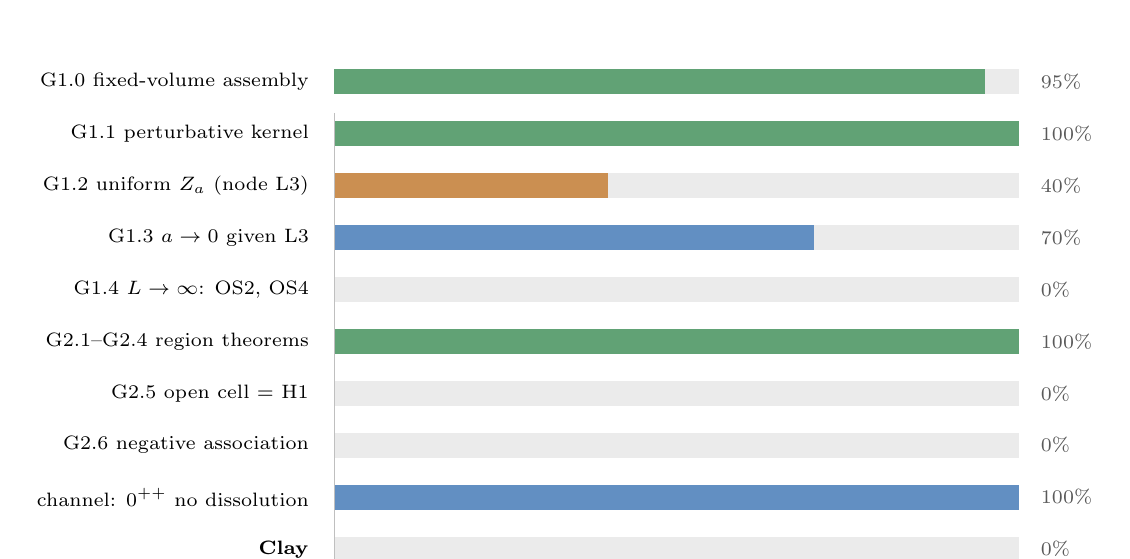
\begin{tikzpicture}[x=1cm,y=1cm,font=\scriptsize]
  \foreach \k/\nm/\pct/\cl in {%
    0/{G1.0 fixed-volume assembly}/95/cT,
    1/{G1.1 perturbative kernel}/100/cT,
    2/{G1.2 uniform $Z_a$ (node L3)}/40/cM,
    3/{G1.3 $a\to0$ given L3}/70/cC,
    4/{G1.4 $L\to\infty$: OS2, OS4}/0/cM,
    5/{G2.1--G2.4 region theorems}/100/cT,
    6/{G2.5 open cell $=$ H1}/0/cM,
    7/{G2.6 negative association}/0/cM,
    8/{channel: $0^{++}$ no dissolution}/100/cC,
    9/{\textbf{Clay}}/0/cN}{
    \pgfmathsetmacro{\yy}{-0.66*\k}
    \node[anchor=east] at (6.3,\yy) {\nm};
    \fill[black!8] (6.5,\yy-0.16) rectangle (15.2,\yy+0.16);
    \pgfmathsetmacro{\ww}{8.7*\pct/100}
    \ifnum\pct>0
      \fill[\cl!70] (6.5,\yy-0.16) rectangle ({6.5+\ww},\yy+0.16);
    \fi
    \node[anchor=west, text=black!65] at (15.35,\yy) {\pct\%};
  }
  \draw[black!25] (6.5,-0.4) -- (6.5,-6.1);
\end{tikzpicture}
\caption{Node board. Percentages are \emph{node-local} --- progress toward each node's own
goal --- and are emphatically not a percentage proof of Clay. Clay is $0\%$ because the
species is unbuilt.}
\label{fig:bars}
\end{figure}
}

% ---------------------------------------------------------------------
% Fig 5 — immune map funnel
% ---------------------------------------------------------------------
\newcommand{\figfunnel}{%
\begin{figure}[t]
\centering
\begin{tikzpicture}[x=1cm,y=1cm]
  \foreach \k/\nm in {%
    0/{positivity / analyticity-only},
    1/{cross-channel protection},
    2/{non-abelian sign calculus},
    3/{wrong half: UV control},
    4/{rename $=$ gap},
    5/{upper-bound direction},
    6/{strong-coupling only},
    7/{index $=0$},
    8/{exact reduction / duality},
    9/{constructive coercivity},
    10/{new inequality / capacity},
    11/{fixed-cell localization},
    12/{transport / monotone},
    13/{lower-bound machines},
    14/{Feshbach / Krein},
    15/{$k=0$ effective curvature},
    16/{Bethe--Salpeter two-gluon},
    17/{string tension $\to$ glueball}}{
    \pgfmathsetmacro{\yy}{-0.43*\k}
    \node[anchor=east, font=\scriptsize, text=black!75] at (6.15,\yy) {\nm};
    \draw[black!28, very thin] (6.28,\yy) -- (9.25,-3.55);
  }
  \node[fbox, text width=5.9cm, fill=cM!7, draw=cM!65] at (12.45,-3.55)
    {\textbf{ONE SPECIES}\\[2pt]
     $\operatorname{Var}_\mu(\langle v,\nabla S\rangle\mid0)\;\le\;E_\mu[H_{vv}\mid0]+W_{\mathrm{full}}-\delta$\\[2pt]
     \scriptsize uniform in $(L,U')$: this is H1 in the infrared and L3 in the ultraviolet};
\end{tikzpicture}
\caption{The immune map. Eighteen root families, spanning roughly ninety distinct routes, all
terminate at the same inequality. This is near theorem-grade \emph{exhaustiveness evidence} ---
not a theorem and not a proof, but a structural fact about where the difficulty lives.}
\label{fig:funnel}
\end{figure}
}

% ---------------------------------------------------------------------
% Fig 6 — one species, two scales
% ---------------------------------------------------------------------
% The one-species figure is emitted by two chapters (intro and ch03). The body is shared, so the
% label is written on the first inclusion only: one \label per key, and \ref{fig:scales} stays
% single-valued (it resolves to the first figure, which is also where the intro cites it).
\newif\ifscaleslabelled
\newcommand{\figscales}{%
\begin{figure}[t]
\centering
\begin{tikzpicture}[x=1cm,y=1cm]
  \node[fbox, text width=13.6cm, fill=cM!7, draw=cM!60] (species) at (7.0,4.6)
    {\textbf{One inequality: a single-sided upper bound on a conditioned variance}\\[2pt]
     \small nonperturbative \quad$\cdot$\quad non-circular \quad$\cdot$\quad free-field-failing
     \quad$\cdot$\quad $(L,a)$-uniform};
  \node[fbox, text width=5.3cm, fill=cC!8, draw=cC!50] (ir) at (3.6,1.4)
    {\textbf{Infrared face: H1}\\ $\operatorname{Var}(\xi_{k\to0})\le 1/\lambda$\\ G2's open cell \ \LM};
  \node[fbox, text width=5.3cm, fill=cC!8, draw=cC!50] (uv) at (10.4,1.4)
    {\textbf{Ultraviolet face: L3}\\ $\sup_a Z_a^{-1}\lVert H_a\rVert_D<\infty$\\ G1's open node \ \LM};
  \draw[arr] (species.south) -- (ir.north);
  \draw[arr] (species.south) -- (uv.north);
  \draw[{Stealth[length=5pt]}-{Stealth[length=5pt]}, draw=cC!60, thick, dashed]
    (ir.east) -- (uv.west);
  \node[font=\scriptsize, text=black!65] at (7.0,2.55) {same shape};
\end{tikzpicture}
\caption{The one-species reduction. The same inequality appears at two scales: as the UV
force-variance bound L3 and as the IR conditioned-variance bound H1. The shapes coincide because
$\operatorname{Var}\ge0$ can only supply a lower edge, while in
$G''=E[H]-\operatorname{Var}+W_{\mathrm{full}}$ the variance subtracts. The unification is a conjecture; the
dictionaries (Ward, residue--level-gap, $G''=E[H]-\operatorname{Var}+W_{\mathrm{full}}$) are theorems, and
building the inequality would close L3 and H1 simultaneously.}
\ifscaleslabelled\else\label{fig:scales}\fi
\end{figure}%
\global\scaleslabelledtrue
}

% ---------------------------------------------------------------------
% Fig 7 — numerics: curvature probe with error bars
% ---------------------------------------------------------------------
\newcommand{\figprobe}{%
\begin{figure}[t]
\centering
\begin{tikzpicture}[x=1cm,y=1cm,font=\scriptsize]
  % axes: y from -0.1 to 0.55
  \draw[arr] (0.8,-0.1*5.4-0.4) -- (0.8,0.58*5.4) ; % y axis
  \draw[arr] (0.8,-0.1*5.4-0.4) -- (9.4,-0.1*5.4-0.4) node[alab, right] {};
  \pgfmathsetmacro{\yzero}{0*5.4-0.0}
  \draw[dashed, black!50] (0.8,{0.0}) -- (9.2,{0.0});
  \node[anchor=east, text=black!60] at (0.7,0.0) {$0$};
  \node[anchor=east, text=black!60] at (0.7,{0.5*5.4}) {$0.5$};
  \node[anchor=east, text=black!55, rotate=90] at (0.15,{0.27*5.4}) {$G''$};
  % data
  \foreach \x/\val/\err/\nm in {2/0.425/0.084/{$L=4$, $k=\pi/2$},
                                4/0.307/0.055/{$L=8$, $k=\pi/4$},
                                6/0.396/0.063/{$L=8$, $k=\pi/2$},
                                8/0.319/0.005/{$W_{\rm geo}$}}{
    \pgfmathsetmacro{\ym}{(\val-\err)*5.4}
    \pgfmathsetmacro{\yp}{(\val+\err)*5.4}
    \pgfmathsetmacro{\yc}{\val*5.4}
    \draw[thick, cC!80] (\x,\ym) -- (\x,\yp);
    \draw[thick, cC!80] (\x-0.09,\ym) -- (\x+0.09,\ym);
    \draw[thick, cC!80] (\x-0.09,\yp) -- (\x+0.09,\yp);
    \fill[cC!85] (\x,\yc) circle (1.6pt);
    \node[rotate=30, anchor=north east, text=black!70, inner sep=1.5pt]
      at ({\x+0.12},-1.05) {\nm};
    \node[above=3pt, text=black!70] at (\x,{\yp+0.02}) {$\val$};
  }
\end{tikzpicture}
\caption{The $k\to0$ curvature probe on a single $L=8$ volume ($\mathrm{SU}(3)$, $\beta=5.7$),
with an $\mathrm{SU}(3)$ $L=4$ check; all plotted points are $\mathrm{SU}(3)$, while
$\mathrm{SU}(2)$ ($\beta=2.4$) reproduces the sign without being plotted. The measured points are positive and volume-stable,
and $W_{\mathrm{geo}}$ is pinned at $+0.32$. This is a $k\to0$ sign probe on a
gauge-dependent gluon mode in a flat chart, \emph{not} the gauge-invariant $0^{++}$ residue;
keeping only the proven $W_{\mathrm{geo}}\ge0$ and treating the rest statistically gives
$95\%$ one-sided lower bounds of $-0.098$ ($\mathrm{SU}(3)$) and $-0.035$ ($\mathrm{SU}(2)$),
so zero is not excluded. Label \LE.}
\label{fig:probe}
\end{figure}
}

% =====================================================================
%  New figures for v2 (styles fbox/arr/alab come from figures-old.tex)
% =====================================================================

% ---------------------------------------------------------------------
% Fig v2-1 — the wall in two coordinates
% ---------------------------------------------------------------------
\newcommand{\figtwocoord}{%
\begin{figure}[t]
\centering
\begin{tikzpicture}[x=1cm,y=1cm]
  \node[fbox, fill=cC!9, draw=cC!60, text width=6.5cm,
        minimum height=3.0cm, align=center] (c1) at (3.2,3.6)
    {\textbf{Coordinate 1}\\[1pt]\textbf{measure / weak-$*$}\\[3pt]
     \scriptsize $\nu\ge0$;\ \ $f_1^2=\nu(\{m_1^2\})$\\[1pt]
     atom $=$ weak-$*$ discontinuity\\[1pt]
     tools: spectral, moments,\\[1pt]
     complex analysis, transport, dependence};
  \node[fbox, fill=cM!9, draw=cM!60, text width=6.5cm,
        minimum height=3.0cm, align=center] (c2) at (10.4,3.6)
    {\textbf{Coordinate 2}\\[1pt]\textbf{$\beta$ / RG / conformal}\\[3pt]
     \scriptsize $\beta_{N_f=0}(g)$;\ \ window $9\le N_f\le16$\\[1pt]
     gap $=$ ``$N_f=0$ outside the window''\\[1pt]
     tools: bootstrap, $a$-theorem,\\[1pt]
     large-$N$, holography, DSE};
  \node[fbox, fill=cN!8, draw=cN!65, text width=10.6cm,
        minimum height=1.6cm, align=center] (wall) at (6.8,0.55)
    {\textbf{ONE INVARIANT}\\[1pt]
     $H1$: the $a\to0$, $L\to\infty$ isolation of the $0^{++}$ atom\\[1pt]
     \scriptsize an upper bound on a conditioned variance, written twice};
  \draw[arr] (3.2,2.15) -- (4.5,1.40);
  \draw[arr] (10.4,2.15) -- (9.1,1.40);
  \node[font=\scriptsize, text=black!60, align=center] at (6.8,5.35)
    {Two disjoint toolboxes; neither closes the wall.};
\end{tikzpicture}
\caption{The campaign's final structural image. The gap is reached from two independent,
non-overlapping coordinates. In the measure coordinate the atom is a weak-$*$ discontinuity and
every finite datum is weak-$*$ continuous, so no positive-measure argument can force it. In the
$\beta$ coordinate the gap is the dynamical statement that pure Yang--Mills lies outside the
conformal window; the window is real, so no kinematic argument can force it either. Both
coordinates terminate at the same invariant. The left arrow denotes ``blind to the atom
(weak-$*$)''; the right arrow denotes ``reduces to the dynamics ($\beta$).''}
\label{fig:twocoord}
\end{figure}
}

% ---------------------------------------------------------------------
% Fig v2-2 — the weak-* dichotomy
% ---------------------------------------------------------------------
\newcommand{\figweakstar}{%
\begin{figure}[t]
\centering
\begin{tikzpicture}[x=1cm,y=1cm,font=\scriptsize]
  \node[fbox, fill=black!4, text width=5.2cm, minimum height=2.9cm] (data) at (2.7,4.3)
    {\textbf{finite data}\\[2pt]
     moments $M_k$ \ \textperiodcentered\ Taylor $c_n$\\
     point evaluations $\Pi(z_j)$\\
     bounded-kernel integrals $\int\varphi\,d\nu$\\
     Wilson-loop $\nu$-images};
  \node[fbox, fill=cT!8, draw=cT!55, text width=4.3cm, minimum height=1.5cm] (cont) at (2.7,1.35)
    {\textbf{all weak-$*$ continuous}};
  \node[fbox, fill=cN!8, draw=cN!60, text width=4.6cm, minimum height=1.5cm] (discont) at (9.7,1.35)
    {\textbf{atom $f_1^2>0$}\\ $=$ weak-$*$ \textbf{discontinuity}};
  \node[fbox, fill=black!4, text width=4.9cm, minimum height=1.5cm] (dense) at (9.7,4.3)
    {\textbf{atomless measures are weak-$*$ dense}\\
     a bump of width $h$ matches any finite data to $O(h)$};
  \draw[arr] (data.south) -- (cont.north);
  \draw[arr] (dense.south) -- (discont.north);
  \draw[{Stealth[length=5pt]}-{Stealth[length=5pt]}, draw=cN!65, thick] (cont.east) -- (discont.west)
    node[alab, above, pos=0.5] {cannot reach};
  \node[fbox, fill=cM!7, draw=cM!60, text width=5.4cm, minimum height=1.7cm] (exit) at (6.2,-0.55)
    {\textbf{any forcing functional is weak-$*$ discontinuous}\\[1pt]
     $\Rightarrow$ either A3 (read across $\mathbb{R}$)\\
     or $J\to\infty$ (all data) $=$ H1};
  \draw[arr] (discont.south) -- (exit.north);
\end{tikzpicture}
\caption{The weak-$*$ dichotomy behind every failed tool. Finite data determine the measure only
weak-$*$; the atom is precisely the failure of weak-$*$ continuity. Atomless measures are weak-$*$
dense, so no finite sample can distinguish an atom from a thin bump. A functional that forces the
atom must therefore be weak-$*$ discontinuous, and is not finitely computable: it either reads the
boundary value (A3) or requires the full limit (H1).}
\label{fig:weakstar}
\end{figure}
}

% ---------------------------------------------------------------------
% Fig v2-3 — the SU(3) conformal window and where N_f = 0 sits
% ---------------------------------------------------------------------
\newcommand{\figwindow}{%
\begin{figure}[t]
\centering
\begin{tikzpicture}[x=1cm,y=1cm,font=\scriptsize]
  \draw[arr] (0,0) -- (13.4,0) node[alab, right] {$N_f$};
  \foreach \x/\l in {0.8/0, 6.0/8, 7.6/10, 9.2/12, 10.8/14, 12.4/16}{
    \draw (\x,0) -- (\x,-0.09) node[below, text=black!65] {\l};
  }
  % AF region
  \fill[cC!12] (0.8,0.25) rectangle (12.9,2.4);
  \node[text=cC!70] at (2.6,2.0) {asymptotically free};
  % window 9..16
  \fill[cT!18] (6.6,0.25) rectangle (12.4,2.4);
  \node[text=cT!75, align=center] at (9.5,1.85) {\textbf{conformal window}\\ $9\le N_f\le16$ (2-loop)};
  \node[text=cT!75, align=center] at (9.5,1.05) {$N_f^c\approx8.05\to11\to12$\\ (2, 4, 5 loops)};
  % confining side
  \fill[cM!10] (0.8,0.25) rectangle (6.0,2.4);
  \node[text=cM!80, align=center] at (3.3,1.55) {confining};
  % N_f=0 marker
  \draw[cN!80, very thick] (0.8,0.25) -- (0.8,2.6);
  \node[cN!85, above, align=center] at (1.55,2.55) {\textbf{$N_f=0$ (pure YM)}};
  \draw[{Stealth[length=5pt]}-{Stealth[length=5pt]}, draw=cN!70, thick]
    (0.95,0.55) -- (6.55,0.55) node[alab, below, pos=0.5] {distance $\approx9$--$12$ units of $N_f$};
  \node[text=black!60] at (11.6,0.0) [above right] {$16.5$: AF ends};
\end{tikzpicture}
\caption{The Banks--Zaks conformal window for $\mathrm{SU}(3)$ with $N_f$ massless fundamentals.
The window is real: those theories are asymptotically free, single-coupling, and gapless in the
infrared. Pure Yang--Mills sits at $N_f=0$, a distance of nine to twelve units of $N_f$ below the
perturbative boundary, while the loop-by-loop shift of that boundary is about $+3$. Hence the
question is not marginal --- but ``$N_f=0$ is outside the window'' is rigorous only
perturbatively; its nonperturbative form is exactly $(G1)$.}
\label{fig:window}
\end{figure}
}

% ---------------------------------------------------------------------
% Fig v2-4 — anatomy of the Savvidy cell
% ---------------------------------------------------------------------
\newcommand{\figsavcell}{%
\begin{figure}[t]
\centering
\begin{tikzpicture}[x=1cm,y=1cm,font=\scriptsize]
  % potential
  \draw[arr] (-0.2,0) -- (8.6,0) node[alab, right] {$\varphi$};
  \draw[arr] (0,0) -- (0,3.6) node[alab, above] {$V_{\mathrm{eff}}$};
  \draw[thick, cC!75, domain=0.4:8.0, samples=80]
    plot (\x,{0.55*(\x-4.2)^2*0.45 - 0.9*exp(-0.9*(\x-4.2)^2) + 1.05});
  \fill[cN!80] (4.2,0.62) circle (1.7pt);
  \node[cN!85, above] at (4.2,0.72) {barrier top: negative mode};
  \fill[cT!80] (2.35,1.55) circle (1.7pt);
  \fill[cT!80] (6.05,1.55) circle (1.7pt);
  \node[cT!80, above] at (2.35,1.62) {$\varphi=-v$};
  \node[cT!80, above] at (6.05,1.62) {$\varphi=+v$};
  \draw[cT!70, thick] (2.35,1.55) -- (2.35,0.0);
  \draw[cT!70, thick] (6.05,1.55) -- (6.05,0.0);
  \node[text=black!60, align=center] at (4.2,-0.55) {true vacuum at $\pm v$: $V''=2c>0$, stable};
  % inset D/S
  \begin{scope}[shift={(8.9,0.7)}]
    \draw[arr] (0,0) -- (3.9,0) node[alab, right] {mode};
    \draw[arr] (0,0) -- (0,2.6) node[alab, above] {$D/S$};
    \draw[dashed, black!45] (0,2.25) -- (3.7,2.25);
    \node[anchor=east, text=black!55] at (-0.05,2.25) {$1$};
    \foreach \x/\v in {0.6/1.02, 1.3/0.97, 2.0/0.99, 2.7/0.94, 3.4/1.00}{
      \fill[cM!85] (\x,{2.25*\v}) circle (1.3pt);
    }
    \node[text=black!60, align=center] at (1.95,-0.5) {near-critical:\\ $D/S\approx0.94$--$1.00$};
  \end{scope}
\end{tikzpicture}
\caption{Anatomy of the Savvidy cell. The negative mode is the barrier-top artifact of the
one-loop effective potential, not a property of the true vacuum at $\varphi=\pm v$, where the
curvature is positive. The softening it produces is bounded, $c$-independent, sign-protected at
two loops, and $(L,a)$-uniform by one-octave support. What survives is a near-critical margin:
the measured defect ratio $D/S$ is $0.94$--$1.00$, sign-fluctuating mode by mode, with the
$k\to0$ mode unmeasured. Establishing that the margin is positive uniformly is H1.}
\label{fig:savcell}
\end{figure}
}

% ---------------------------------------------------------------------
% Fig v2-5 — the two diagnostics: approach law and finite-size law
% ---------------------------------------------------------------------
\newcommand{\figdiag}{%
\begin{figure}[t]
\centering
\begin{tikzpicture}[x=1cm,y=1cm,font=\scriptsize]
  % panel A: T(tau)
  \begin{scope}
    \draw[arr] (0,0) -- (6.4,0) node[alab, right] {$\tau$};
    \draw[arr] (0,0) -- (0,3.3) node[alab, above] {$T(\tau)$};
    \draw[thick, cT!80, domain=0.25:6.0, samples=60]
      plot (\x,{1.55 - 0.9*exp(-\x/1.3)});
    \draw[thick, cN!75, dashed, domain=0.25:6.0, samples=60]
      plot (\x,{0.55/\x});
    \node[cT!80, right] at (5.3,1.72) {atom: $T\to\Delta$};
    \node[cN!80, anchor=west] at (4.35,0.30) {cut: $T\to1/\tau$};
    \node[text=black!60, align=center] at (3.1,-0.6) {P3 approach law};
  \end{scope}
  % panel B: Delta(L)
  \begin{scope}[shift={(8.2,0)}]
    \draw[arr] (0,0) -- (6.2,0) node[alab, right] {$1/L^2$};
    \draw[arr] (0,0) -- (0,3.3) node[alab, above] {$\Delta(L)$};
    \draw[thick, cC!80, domain=0.35:5.7, samples=40]
      plot (\x,{0.55 + 0.38*\x});
    \draw[dashed, black!45] (0,0.55) -- (5.8,0.55);
    \node[anchor=east, text=black!55] at (-0.05,0.55) {$m_1$};
    \node[cC!80, anchor=west] at (1.05,2.62) {$\Delta(L)=m_1+\dfrac{c}{m_1L^2}$};
    \node[text=black!60, align=center] at (3.1,-0.6) {finite-size scaling law};
  \end{scope}
\end{tikzpicture}
\caption{The two genuine diagnostics of the $\mathrm{IR}$ atom. Left: the P3 approach law
$T(\tau)=-d\log|m-\hat e_1|/d\tau$ tends to the gap $\Delta$ for an isolated atom and decays as
$1/\tau$ for a pure cut; it is robust to a background continuum and to the choice of operator.
Right: the finite-size law $\Delta(L)=m_1+c/(m_1L^2)$ for an atom versus $(2\pi/L)^2/m\to0$ for a
cut. Both are reads, not certificates: a single finite volume cannot decide, because every
discrete finite-volume spectrum looks exponential, and the discriminating content is the
$L\to\infty$ survival of the isolation, which is H1.}
\label{fig:diag}
\end{figure}
}

% ---------------------------------------------------------------------
% Fig v2-6 — the three coordinates of the strut (roof diagram)
% ---------------------------------------------------------------------
\newcommand{\figroof}{%
\begin{figure}[t]
\centering
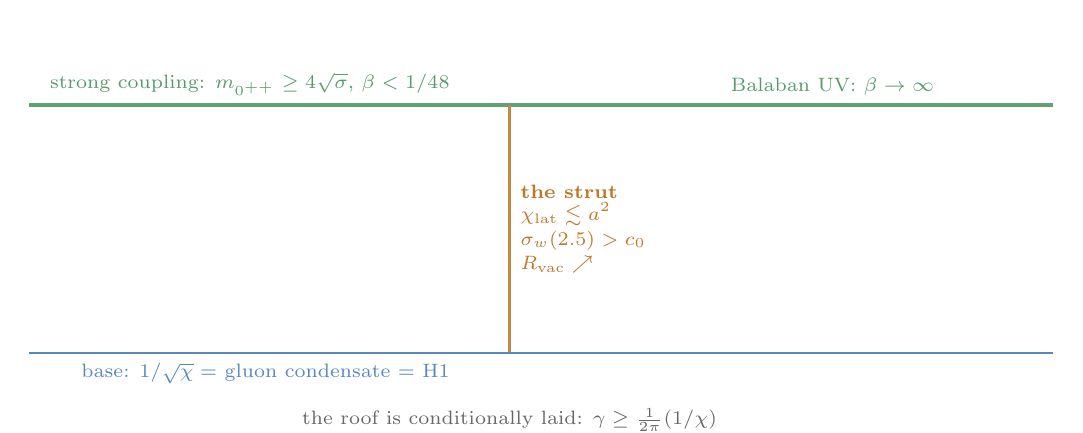
\begin{tikzpicture}[x=1cm,y=1cm,font=\scriptsize]
  \draw[very thick, cT!70] (0.4,3.15) -- (13.4,3.15);
  \node[text=cT!75, above] at (3.2,3.15) {strong coupling: $m_{0^{++}}\ge4\sqrt\sigma$, $\beta<1/48$};
  \node[text=cT!75, above] at (10.6,3.15) {Balaban UV: $\beta\to\infty$};
  \draw[very thick, cM!75] (6.5,0.0) -- (6.5,3.15) node[midway, right, text=cM!85, align=left]
    {\textbf{the strut}\\ $\chi_{\mathrm{lat}}\lesssim a^2$\\[1pt] $\sigma_w(2.5)>c_0$\\[1pt] $R_{\mathrm{vac}}\nearrow$};
  \draw[thick, cC!75] (0.4,0.0) -- (13.4,0.0);
  \node[text=cC!75, below] at (3.4,0.0) {base: $1/\sqrt\chi=$ gluon condensate $=$ H1};
  \node[text=black!60, align=center] at (6.5,-0.85)
    {the roof is conditionally laid: $\gamma\ge\frac{1}{2\pi}(1/\chi)$};
\end{tikzpicture}
\caption{The roof, honestly. Two beams exist at the ends (strong coupling and the ultraviolet);
the base stands; one strut is missing in the middle. The strut has three equivalent names,
depending on the coordinate used to write the susceptibility certificate. It is \emph{not} an
order parameter (zero-temperature pure Yang--Mills is a single phase, so there is nothing to
condense), \emph{not} a topological index (any such index is constant along the connected
coupling family), and \emph{not} a Markov-semigroup functional (homogeneous in the Hessian).}
\label{fig:roof}
\end{figure}
}

% =====================================================================
%  Additional explanatory figures for v2 (vector only, TikZ)
%  Styles fbox / arr / alab are defined in figures-old.tex.
% =====================================================================

% ---------------------------------------------------------------------
% X1 — the three halves feeding Clay
% ---------------------------------------------------------------------
\newcommand{\figthreehalves}{%
\begin{figure}[t]
\centering
\begin{tikzpicture}[x=1cm,y=1cm]
  \node[fbox, fill=cC!8, draw=cC!55, text width=4.3cm, minimum height=2.7cm] (g1) at (2.7,3.5)
    {\textbf{G1 --- existence}\\[2pt]
     \scriptsize 4D continuum, OS0--OS4;\\
     fixed volume assembled\\
     modulo the uniform $Z_a$\\[2pt]
     \LT{} mod.\ L3 \quad \LM{} L3 (UV)};
  \node[fbox, fill=cM!8, draw=cM!60, text width=4.3cm, minimum height=2.7cm] (g2) at (8.0,3.5)
    {\textbf{G2 --- the gap}\\[2pt]
     \scriptsize $f_1^2>0$ with isolation;\\
     equivalently $G''(0)\ge\lambda$\\
     as $k\to0$, $(L,a)$-uniform\\[2pt]
     \LT{} region $\sim$90\% \quad \LM{} sign 0\%};
  \node[fbox, fill=cT!8, draw=cT!55, text width=4.3cm, minimum height=2.7cm] (ch) at (13.3,3.5)
    {\textbf{The channel}\\[2pt]
     \scriptsize lightest state in $0^{++}$;\\
     no-dissolution theorem;\\
     ordering input \code{IN-11}\\[2pt]
     \LC{} conditional};
  \node[fbox, fill=cN!7, draw=cN!55, text width=7.4cm] (clay) at (8.0,0.55)
    {\textbf{Clay: existence $\wedge$ uniform gap}
     \quad\textbf{0\% --- open}};

  \draw[arr] (g1.south) -- (clay.north west);
  \draw[arr] (g2.south) -- (clay.north);
  \draw[arr] (ch.south) -- (clay.north east);
\end{tikzpicture}
\caption{The three objects the campaign separates. G1 is a construction problem, G2 is a lower
bound on the Hamiltonian, and the channel is the identification of the lightest state with the
$0^{++}$ glueball. They feed one conclusion but are neither equivalent nor ordered: a gap does
not give existence, existence does not give a gap, and a gap in some channel does not identify
the channel. Only the middle object is undecided on both its region and its sign.}
\label{fig:threehalves}
\end{figure}
}

% ---------------------------------------------------------------------
% X2 — the research loop
% ---------------------------------------------------------------------
\newcommand{\figloop}{%
\begin{figure}[t]
\centering
\begin{tikzpicture}[x=1cm,y=1cm]
  \node[fbox, fill=cC!8, draw=cC!55, text width=3.6cm] (forge) at (8,5.6)
    {\textbf{1. Forge}\\ a new tool or identity};
  \node[fbox, fill=cE!8, draw=cE!55, text width=3.6cm] (acid) at (12.0,2.9)
    {\textbf{2. Acid test}\\ must fail on the free field};
  \node[fbox, fill=cT!8, draw=cT!55, text width=3.6cm] (audit) at (8,0.2)
    {\textbf{3. Audit}\\ against the source files};
  \node[fbox, fill=cM!8, draw=cM!60, text width=3.6cm] (bank) at (4.0,2.9)
    {\textbf{4. Bank or record}\\ theorem, or exact no-go};

  \draw[arr] (forge) -- node[alab, above right=-1pt] {\scriptsize test} (acid);
  \draw[arr] (acid) -- node[alab, below right=-1pt] {\scriptsize if it survives} (audit);
  \draw[arr] (audit) -- node[alab, below left=-1pt] {\scriptsize verdict} (bank);
  \draw[arr] (bank) -- node[alab, above left=-1pt] {\scriptsize next round} (forge);
  \node[font=\scriptsize, text=black!60, align=center, text width=5.4cm] at (8,2.9)
    {one round\\[2pt] a tool that passes\\ the free field is vacuous};
\end{tikzpicture}
\caption{The working loop imposed by the project charter. Every proposed tool must first fail on
the massless free field (where $f_1^2=0$ and $G''=0$); a tool that ``proves'' a gap there is
vacuous and is discarded. Only then is it run against the campaign's source files, and only then
is it banked as a theorem or recorded as a no-go with the exact point of failure.}
\label{fig:loop}
\end{figure}
}

% ---------------------------------------------------------------------
% X3 — the five labels
% ---------------------------------------------------------------------
\newcommand{\figlabelmap}{%
\begin{figure}[t]
\centering
\begin{tikzpicture}[x=1cm,y=1cm,font=\scriptsize]
  \foreach \x/\col/\chip/\name/\txt in {%
    1.8/cT/\LT/{Theorem}/{proved; imported results are named},
    5.0/cC/\LC/{Conditional}/{proved implication from named hypotheses},
    8.2/cN/\LN/{No-go}/{a whole class cannot work},
    11.4/cM/\LM/{Missing step}/{one open inequality, no slack hidden},
    14.6/cE/\LE/{Evidence}/{measured, not proved}}{%
    \node[fbox, fill=\col!6, draw=\col!45, text width=2.9cm, minimum height=2.5cm]
      at (\x,1.6) {\chip\\[2pt]\textbf{\name}\\[2pt]\txt};}
\end{tikzpicture}
\caption{The five labels used throughout. They are not decoration: each claim carries exactly
one, and the label decides what the claim may be used for. In particular an \LE{} number is never
substituted into a \LT{} statement, and a \LM{} is stated as an inequality with zero slack rather
than as ``work in progress''.}
\label{fig:labelmap}
\end{figure}
}

% ---------------------------------------------------------------------
% X4 — the spectrum ladder
% ---------------------------------------------------------------------
\newcommand{\figladder}{%
\begin{figure}[t]
\centering
\begin{tikzpicture}[x=1cm,y=1cm,font=\scriptsize]
  \draw[arr] (1.0,1.2) -- (15.2,1.2) node[alab, right] {$E$};
  \fill[gray!18] (12.0,1.2) rectangle (15.0,4.2);
  \draw[dashed, black!55] (12.0,1.2) -- (12.0,4.2);
  % levels
  \draw[very thick, black!70] (2.6,1.2) -- (2.6,3.0);
  \node[above] at (2.6,3.0) {$\Omega$ (vacuum)};
  \draw[very thick, cN!85] (6.0,1.2) -- (6.0,3.8);
  \node[above, text=cN!85] at (6.0,3.8) {$0^{++}$ at $m_1$};
  \node[left, text=cN!85] at (5.9,2.6) {height $f_1^2=\nu(\{m_1^2\})$};
  \draw[very thick, black!45] (9.0,1.2) -- (9.0,3.0);
  \node[above, text=black!55] at (9.0,3.0) {$0^{++*}$ at $\approx1.5\,m_1$};
  \node[text=black!60] at (13.5,3.95) {two-glueball};
  \node[text=black!60] at (13.5,3.65) {continuum};
  % brackets
  \draw[decorate, decoration={brace, amplitude=4pt}, cM!85]
    (6.15,2.2) -- node[above=4pt, text=cM!85] {$I_2$ margin $\delta\approx0.5\,m_1$} (8.85,2.2);
  \draw[decorate, decoration={brace, amplitude=4pt, mirror}, black!55]
    (6.15,0.95) -- node[below=4pt] {two-body threshold $2m_1$} (11.85,0.95);
\end{tikzpicture}
\caption{The spectral ladder of the $0^{++}$ channel. The atom weight $f_1^2$ (label I1) is the
height of the first level; the isolation (I2) is its distance to the \emph{excited} scalar, not
to the two-glueball continuum. This distinction is the reason the strong-coupling residue theorem
does not by itself give a gap, and why the operative threshold in the no-dissolution theorem is
$1.5\,m_g$ rather than $2m_g$.}
\label{fig:ladder}
\end{figure}
}

% ---------------------------------------------------------------------
% X5 — the G1 pipeline
% ---------------------------------------------------------------------
\newcommand{\figpipeline}{%
\begin{figure}[t]
\centering
\begin{tikzpicture}[x=1cm,y=1cm,font=\scriptsize]
  \foreach \x/\col/\nm/\txt in {%
    1.6/cT/{L1}/{definition of the measure},
    4.2/cT/{L2}/{single-block bound},
    6.8/cM/{L3}/{uniform $Z_a$},
    9.4/cT/{GL3}/{compactness},
    12.0/cT/{GL4}/{reflection positivity},
    14.5/cT/{OS0--4}/{reconstruction}}{%
    \node[fbox, fill=\col!7, draw=\col!50, text width=2.25cm, minimum height=1.7cm]
      at (\x,1.8) {\textbf{\nm}\\[1pt]\txt};}
  \foreach \a/\b in {1.6/4.2,4.2/6.8,6.8/9.4,9.4/12.0,12.0/14.5}{%
    \draw[arr] (\a+1.15,1.8) -- (\b-1.15,1.8);}
  \node[font=\scriptsize, text=cM!85, align=center, text width=5.4cm] at (6.8,-0.15)
    {the only open UV node: $\sup_a Z_a^{-1}\lVert H_a\rVert_D<\infty$\\ (a single-sided force-variance bound)};
\end{tikzpicture}
\caption{The existence pipeline G1. Every arrow except the third is closed by a theorem or by the
statement of the measure; L3 is the single open ultraviolet node. It is deliberately drawn next
to G2's H1 in the text, because L3 and H1 are the same species of inequality at two different
scales.}
\label{fig:pipeline}
\end{figure}
}

% ---------------------------------------------------------------------
% X6 — isometric lattice with a plaquette and a flux tube
% ---------------------------------------------------------------------
\newcommand{\figlattice}{%
\begin{figure}[t]
\centering
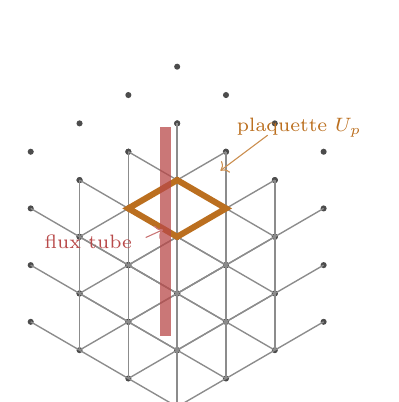
\begin{tikzpicture}[x=1cm,y=1cm,font=\scriptsize,
  X/.style={draw=black!45, line width=0.5pt},
  Xhot/.style={draw=cM!90, line width=2.2pt}]
  % isometric basis
  \def\ex{0.62} \def\ey{0.36}
  \def\fz{0.72}
  % vertices (i,j,k) in 0..3
  \foreach \i in {0,1,2,3}{%
    \foreach \j in {0,1,2,3}{%
      \foreach \k in {0,1,2,3}{%
        \pgfmathsetmacro{\px}{\i*\ex - \j*\ex}
        \pgfmathsetmacro{\py}{\i*\ey + \j*\ey + \k*\fz}
        \fill[black!70] (\px,\py) circle (1.1pt);
      }}}
  % links along x, y, z (only within 0..2)
  \foreach \i in {0,1,2}{%
    \foreach \j in {0,1,2}{%
      \foreach \k in {0,1,2}{%
        \pgfmathsetmacro{\ax}{\i*\ex-\j*\ex} \pgfmathsetmacro{\ay}{\i*\ey+\j*\ey+\k*\fz}
        \pgfmathsetmacro{\bx}{\ax+\ex} \pgfmathsetmacro{\by}{\ay+\ey}
        \draw[X] (\ax,\ay) -- (\bx,\by);
        \pgfmathsetmacro{\cx}{\ax-\ex} \pgfmathsetmacro{\cy}{\ay+\ey}
        \draw[X] (\ax,\ay) -- (\cx,\cy);
        \pgfmathsetmacro{\dx}{\ax} \pgfmathsetmacro{\dy}{\ay+\fz}
        \draw[X] (\ax,\ay) -- (\dx,\dy);
      }}}
  % highlighted plaquette on the top layer (i=0..1, j=0..1, k=3)
  \pgfmathsetmacro{\pax}{0} \pgfmathsetmacro{\pay}{0+0+3*\fz}
  \pgfmathsetmacro{\pbx}{\ex} \pgfmathsetmacro{\pby}{\ey+3*\fz}
  \pgfmathsetmacro{\pcx}{0} \pgfmathsetmacro{\pcy}{2*\ey+3*\fz}
  \pgfmathsetmacro{\pdx}{-\ex} \pgfmathsetmacro{\pdy}{\ey+3*\fz}
  \draw[Xhot] (\pax,\pay) -- (\pbx,\pby) -- (\pcx,\pcy) -- (\pdx,\pdy) -- cycle;
  % flux tube through the centre
  \draw[cN!80, line width=4pt, opacity=0.75] (-0.15,0.9) -- (-0.15,3.55);
  \node[text=cN!80, anchor=east] at (-0.45,2.1) {flux tube};
  \draw[cN!60, ->, thin] (-0.4,2.15) -- (-0.18,2.25);
  \node[text=cM!90] at (1.55,3.55) {plaquette $U_p$};
  \draw[cM!70, ->, thin] (1.15,3.45) -- (0.55,3.0);
\end{tikzpicture}
\caption{A $3^3$ periodic lattice in isometric view: site variables, link variables, one
plaquette $U_p$ (the object whose trace enters the Wilson action and the operator
$\operatorname{tr}F^2$), and a flux tube. The figure fixes the objects used throughout: the
strong-coupling residue theorem counts polymers of such plaquettes, and the no-dissolution
argument is about what a tube of this kind can and cannot do.}
\label{fig:lattice}
\end{figure}
}

% ---------------------------------------------------------------------
% X7 — the variance ledger
% ---------------------------------------------------------------------
\newcommand{\figbalance}{%
\begin{figure}[t]
\centering
\begin{tikzpicture}[x=1cm,y=1cm,font=\scriptsize]
  \draw[arr] (0.8,0.4) -- (0.8,4.6) node[alab, above] {value};
  \draw[dashed, black!45] (0.8,1.1) -- (14.6,1.1);
  % waterfall: E[H] up, Var down, W up, net
  \fill[cT!55] (1.7,1.1) rectangle (3.3,3.3);
  \node[above] at (2.5,3.3) {$E[H]$};
  \fill[cN!45] (4.4,1.3) rectangle (6.0,3.3);
  \node[below] at (5.2,1.3) {$-\operatorname{Var}$};
  \fill[cC!55] (7.1,1.1) rectangle (8.7,1.45);
  \node[above] at (7.9,1.45) {$+W_{\mathrm{full}}$};
  \fill[black!70] (9.8,1.1) rectangle (11.4,1.55);
  \node[above] at (10.6,1.55) {$G''=S-D$};
  \draw[dotted, black!60] (3.3,3.3) -- (4.4,3.3);
  \draw[dotted, black!60] (6.0,1.3) -- (7.1,1.3);
  \draw[dotted, black!60] (8.7,1.45) -- (9.8,1.45);
  \node[align=left, text width=3.4cm] at (13.2,2.6)
    {$G''=E[H]-\operatorname{Var}+W_{\mathrm{full}}$\\[2pt]
     $=\Delta_{\mathrm{dyn}}+W_{\mathrm{geo}}+X$};
  \node[text=black!55] at (5.2,0.55) {schematic heights};
\end{tikzpicture}
\caption{The variance ledger behind the gap. The unconditioned curvature $E[H]$ is large and
positive; the variance of the force subtracts from it; the geometric/cross remainder
$W_{\mathrm{full}}=W_{\mathrm{geo}}+X$ is what is left of the conditioning correction. The sign
of $G''$ is therefore not a statement about the size of $E[H]$ --- that is positive for trivial
reasons --- but about the subtractive variance term, which is exactly the object no known tool
bounds from above at $\beta\approx2.5$. Heights are schematic.}
\label{fig:balance}
\end{figure}
}

% ---------------------------------------------------------------------
% X8 — stable and unstable directions at the Savvidy point
% ---------------------------------------------------------------------
\newcommand{\figsaddle}{%
\begin{figure}[t]
\centering
\begin{tikzpicture}[x=1cm,y=1cm,font=\scriptsize]
  \draw[arr] (0.9,2.0) -- (7.2,2.0) node[alab, right] {$t$};
  \draw[arr] (0.9,0.4) -- (0.9,3.6) node[alab, above] {$V$};
  \draw[cN!85, thick, domain=-2.2:2.2, samples=60] plot ({3.6+1.25*\x},{2.0-0.28*\x*\x});
  \node[text=cN!85, align=left, text width=3.0cm] at (6.0,3.0)
    {negative mode:\\ $\lambda^2<0$ (unstable)};
  \draw[cT!70, thick, domain=-2.2:2.2, samples=60] plot ({11.0+1.25*\x},{2.0+0.28*\x*\x});
  \node[text=cT!70, align=left, text width=3.0cm] at (12.5,0.7)
    {positive modes:\\ stable};
  \node[text=black!60, align=center, text width=4.2cm] at (3.0,0.55)
    {transverse magnetic mode};
  \node[text=black!60, align=center, text width=4.2cm] at (12.6,3.5)
    {would-be convex directions};
\end{tikzpicture}
\caption{The Savvidy phenomenon in one dimension. Around a constant chromomagnetic background the
effective potential is concave along the transverse magnetic mode and convex along the others.
The concavity is physical, not a gauge artifact: it survives the gauge quotient, and it is the
reason every convexity-based tool (Pr\'ekopa, Brascamp--Lieb, log-concavity) stops at the
background. The campaign's $W_{\mathrm{geo}}\ge0$ theorem controls the Haar part, not this term.}
\label{fig:saddle}
\end{figure}
}

% ---------------------------------------------------------------------
% X9 — the theorem dependency graph
% ---------------------------------------------------------------------
\newcommand{\figproofdag}{%
\begin{figure}[t]
\centering
\begin{tikzpicture}[x=1cm,y=1cm,font=\scriptsize]
  \foreach \x/\col/\nm/\lab in {%
    1.7/cM/{H1}/\LM,
    4.9/cC/{CP}/\LC,
    8.1/cT/{$W_{\mathrm{geo}}\!\ge0$}/\LT,
    11.3/cT/{P3}/\LT,
    14.5/cC/{no-diss.}/\LC}{%
    \node[fbox, fill=\col!7, draw=\col!50, text width=2.7cm] at (\x,4.2)
      {\textbf{\nm}\\[1pt]\lab};}
  \node[fbox, fill=cT!10, draw=cT!60, text width=9.6cm] (red) at (8.0,1.9)
    {\textbf{conditional reduction (Lean 4)}\\[2pt]
     \code{clay\_gap\_conditional} : H1 $\wedge$ CP $\wedge$ $W_{\mathrm{geo}}\!\ge0$ $\wedge$ P3
     $\wedge$ no-diss. $\Longrightarrow$ $\Delta>0$\\[2pt]
     zero \code{sorryAx}; the five inputs are explicit hypotheses};
  \node[fbox, fill=cN!8, draw=cN!55, text width=9.6cm] (clay) at (8.0,0.25)
    {\textbf{Clay} \quad 0\% --- open: the five inputs are unproved};
  \draw[arr] (8.1,3.55) -- (red.north);
  \draw[arr] (11.3,3.55) -- (red.north east);
  \draw[arr] (4.9,3.55) -- (red.north west);
  \draw[arr] (1.7,3.55) -- (red.north west);
  \draw[arr] (14.5,3.55) -- (red.north east);
  \draw[arr] (red.south) -- (clay.north);
\end{tikzpicture}
\caption{What the Lean development does and does not certify. The reduction is machine-checked:
if the five analytic facts hold, then the gap follows, and the proof uses only the standard
axioms. The five facts are hypotheses, not theorems in Lean; three of them are theorems in the
paper (P3, $W_{\mathrm{geo}}\ge0$, no-dissolution), while H1 and (CP) are open. The diagram is
the precise sense in which ``the logic is verified, the inputs are not''.}
\label{fig:proofdag}
\end{figure}
}

% ---------------------------------------------------------------------
% X10 — moments versus determinant
% ---------------------------------------------------------------------
\newcommand{\figfredholm}{%
\begin{figure}[t]
\centering
\begin{tikzpicture}[x=1cm,y=1cm,font=\scriptsize]
  % panel A: the measure
  \draw[arr] (0.9,0.7) -- (6.9,0.7) node[alab, right] {$s$};
  \fill[black!75] (2.4,0.7) rectangle (2.55,2.5);
  \node[above] at (2.47,2.5) {$f_1^2$};
  \fill[gray!25] (3.2,0.7) -- (3.2,1.55) -- (4.2,1.25) -- (5.4,1.0) -- (6.6,0.85) -- (6.6,0.7) -- cycle;
  \node[text=black!60] at (5.0,1.55) {cut};
  \node[text=black!60, align=center, text width=5.2cm] at (3.8,3.65)
    {moments $\int s^k\,d\nu$ see atom and cut alike};
  % panel B: the complex z-plane
  \begin{scope}[shift={(9.4,0)}]
    \draw[arr] (0.2,1.6) -- (5.8,1.6) node[alab, right] {$\Re z$};
    \draw[arr] (3.0,0.35) -- (3.0,2.9) node[alab, above] {$\Im z$};
    \draw[black!45, thick] (3.0,1.6) circle (1.0);
    \node[text=black!55] at (4.55,2.75) {$|z|=1$ (cut)};
    \draw[cN!85, very thick] (4.35,1.6) -- (4.75,1.6);
    \draw[cN!85, very thick] (4.55,1.4) -- (4.55,1.8);
    \node[text=cN!85, below] at (4.55,1.35) {$z_1=e^{am_1}$};
    \node[text=black!60, align=center, text width=5.4cm] at (2.9,3.75)
      {the determinant has a zero at $z_1$ and none elsewhere inside the cut};
  \end{scope}
  \node[text=black!60, align=center, text width=15cm] at (7.7,-0.05)
    {same lower moments, different zero sets: the Fredholm determinant is linear-blind but sees the atom};
\end{tikzpicture}
\caption{Why the Fredholm determinant is the only tool of the six that ``sees'' the atom. Every
moment of the measure --- including all the moments the squeeze uses --- is blind to whether the
bottom of the spectrum is an atom or the edge of a cut. The determinant $\det(1-zT_O)$ is not:
a pole of the resolvent produces a zero at $z_1=e^{am_1}$, a cut produces none. The price is
that the zero has to be followed to $a\to0$.}
\label{fig:fredholm}
\end{figure}
}

% ---------------------------------------------------------------------
% X11 — the verdict card
% ---------------------------------------------------------------------
\newcommand{\figverdictcard}{%
\begin{figure}[t]
\centering
\begin{tikzpicture}[x=1cm,y=1cm,font=\scriptsize]
  \node[fbox, fill=cN!8, draw=cN!60, text width=15.2cm, minimum height=0.9cm] at (7.8,3.9)
    {\textbf{Clay: 0\% --- open.} \ The wall is located and instrumented, not crossed.};
  \foreach \x/\col/\big/\small in {%
    1.9/cT/{100\%}/{G1 assembled\\ modulo $\{L3,G2\}$},
    5.7/cC/{100\%}/{channel pinned\\ (conditional)},
    9.5/cM/{90\% / 0\%}/{G2 region / G2 sign},
    13.3/cM/{6 / 7}/{tools passing\\ acid test / no-gos}}{%
    \node[fbox, fill=\col!7, draw=\col!50, text width=3.3cm, minimum height=2.0cm]
      at (\x,1.9) {\textbf{\big}\\[2pt]\small};}
  \node[text=black!55, align=center, text width=15cm] at (7.8,0.35)
    {the missing object: one single-sided, cutoff-uniform upper bound on a conditioned variance};
\end{tikzpicture}
\caption{The verdict in five numbers. None of them is a percentage of Clay; each is local to its
own object. The two zeros matter more than the three high numbers: G2's sign and the missing
tool are the same absence, and the other numbers only say that everything around it is
assembled.}
\label{fig:verdictcard}
\end{figure}
}

% ---------------------------------------------------------------------
% X12 — the Lean dependency tree
% ---------------------------------------------------------------------
\newcommand{\figlean}{%
\begin{figure}[t]
\centering
\begin{tikzpicture}[x=1cm,y=1cm,font=\scriptsize]
  \node[fbox, fill=cT!10, draw=cT!60, text width=6.8cm] (root) at (8.0,5.5)
    {\code{mass\_gap\_of\_spectral} \quad proved};
  \foreach \x/\nm/\lab/\st in {%
    1.7/{H1\_holds}/{H1}/\LM,
    4.85/{CP\_holds}/{CP}/\LC,
    8.0/{W\_geo\_nonneg\_fact}/{W$_{\mathrm{geo}}\!\ge0$}/\LT,
    11.15/{P3\_strong\_coupling}/{P3}/\LT,
    14.3/{no\_dissolution\_kinematic}/{no-diss.}/\LC}{%
    \node[fbox, fill=cM!8, draw=cM!55, text width=2.8cm, minimum height=1.35cm] at (\x,3.4)
      {\textbf{\lab}\\[1pt]{\tiny\texttt{\nm}}\\[1pt]\textcolor{cM!85}{\st}};
    \draw[arr] (\x,4.1) -- (root.south);}
  \node[fill=black!4, rounded corners=2pt, draw=black!25, text width=11.0cm,
        font=\scriptsize, align=center] (ax) at (8.0,1.35)
    {axioms of \code{clay\_gap\_conditional}:
     \code{[propext, Classical.choice, Quot.sound]} --- no \code{sorryAx}};
\end{tikzpicture}
\caption{The Lean dependency tree. The root lemma is proved; the five leaves are \code{sorry}
hypotheses with the exact analytic statements of the paper. What the machine certifies is the
assembling of the leaves into the gap, not the leaves themselves. This is the formal counterpart
of the label system: a \LT{} inside Lean is a proved lemma, and a \LM{} is a \code{sorry} whose
statement has been fixed.}
\label{fig:lean}
\end{figure}
}


% =====================================================================
\clearpage
\part{The reduction}
% =====================================================================
\section{Introduction}

\label{sec:intro}
% =====================================================================

\subsection{The Clay statement, exactly}

The Clay problem, as posed by Jaffe and Witten, is:

\begin{qbox}
Prove that for any compact simple gauge group $G$, a non-trivial quantum Yang--Mills theory
exists on $\mathbb{R}^4$ and has a mass gap $\Delta>0$. Existence includes establishing
axiomatic properties at least as strong as those cited in Streater--Wightman (1964) and
Osterwalder--Schrader (1973, 1975). [Jaffe--Witten, \emph{Quantum Yang--Mills Theory}, Clay
Mathematics Institute]
\end{qbox}

Three features of this statement are habitually under-weighted and drive everything that follows.

\textbf{(1) Uniformity.} It demands a uniform gap: not merely that each finite lattice volume has
a positive spectral gap (trivially true by compactness), but that the gap survives $L\to\infty$
and $a\to0$ with a volume- and cutoff-uniform lower bound, and that the resulting theory clusters
exponentially at a rate $m>0$ in every channel carrying the lightest state.

\textbf{(2) Gauge invariance.} It demands that the gap be a feature of the gauge-invariant,
physical theory --- not of a gauge-fixed chart, and not of a perturbative expansion around a
chosen background. This sounds like a technicality; it is not. Several of the campaign's
apparent ``positive signals'' turned out to live on gauge-dependent modes, and one of the
no-gos below is precisely that gauge invariance reaches the vacuum but not the first excited
scalar.

\textbf{(3) Existence plus gap are logically separate.} A construction of the measure with the
Osterwalder--Schrader axioms (existence) is a different task from the lower bound on the
Hamiltonian (gap). They interact --- a uniform gap gives clustering, and clustering is one of the
axioms --- but neither implies the other. The campaign treats them as two halves, G1 and G2, and
is explicit that progress on one does not constitute progress on the other.

\figthreehalves

The campaign's operational form of the Clay conclusion, assembled and partially machine-verified
in \code{docs/conditional-theorem.md}, is:
\begin{align*}
&\exists\,\mu\ \text{on}\ \mathbb{R}^4,\ \text{gauge-invariant, satisfying OS0--OS4};\\
&\text{non-Gaussian},\quad g_{\mathrm{ren}}/\Lambda>0;\\
&\Delta/\Lambda\ \ge\ \min(\delta_W,\delta_S)>0;\\
&|S(f\,\tau_a g)-S(f)\,S(g)|\ \le\ C\,e^{-m\|a\|},\qquad
  m\ge c\,\Delta>0,\ \ \text{all gauge-invariant local } f,g;\\
&\text{unique vacuum};\quad \text{area law } \sigma=c_\sigma\Lambda^2>0;\quad
  \text{all constants group-uniform in } (h^{\vee},\dim G,\dim\mathfrak{g}).
\end{align*}

The transfer-matrix form of the same statement is the one used throughout this paper. For the
lattice transfer matrix $T_a=e^{-H_a}$ on the gauge-invariant Hilbert space $\mathcal{H}_a$, with
vacuum $\Omega$,
\begin{equation}
\exists\,\delta>0:\qquad
\inf\operatorname{spec}\!\bigl(H_a\big|_{\Omega^\perp}\bigr)\ \ge\ \delta\Lambda
\qquad\text{for all sufficiently small } a .
\label{eq:clay-transfer}
\end{equation}
The operator $T_a$ is a positive, positivity-improving operator on $\mathcal{H}_a$ at every
$\beta>0$ (the transfer-matrix theorem of \S\ref{thm:pf}); the Clay content is that its first eigenvalue gap does not
collapse as $a\to0$ and $L\to\infty$.

\subsection{The lock-core rewriting}

The campaign works with a sharper, channel-specific rewriting of the gap which, while not
literally equivalent to the Clay statement, is the correct object to attack. Let $\nu$ be the
K\"all\'en--Lehmann spectral measure of the gauge-invariant local operator
$O=\operatorname{tr}F^2$ (more precisely $O_S=\tfrac14\operatorname{tr}F_{\mu\nu}F^{\mu\nu}$,
the scalar density; the normalization is immaterial). Reflection positivity gives $\nu\ge0$
and $\operatorname{supp}\nu\subset[m_1^2,\infty)$, where $m_1$ is the lightest mass in the
$0^{++}$ channel. The \textbf{atom} is
\begin{equation}
f_1^2 \;:=\; \nu(\{m_1^2\}) \;=\; \bigl|\langle 0|\operatorname{tr}F^2|\mathbb{G}\rangle\bigr|^2 ,
\label{eq:atom}
\end{equation}
the squared overlap of the vacuum with the lightest $0^{++}$ glueball $\mathbb{G}$. The
\textbf{lock core} is: $f_1^2>0$ and the atom is isolated ($\Delta>0$ above it). The campaign
summarises this as
\begin{equation}
\text{Clay}\iff\neg(\mathrm{iii}),\qquad
(\mathrm{iii})=\text{``the YM measure is a gapless interacting 4D CFT''.}
\label{eq:lockcore}
\end{equation}

This rewriting is useful because it names the exact analytic object (an atom weight in a positive
measure at the bottom of a channel) and the exact analytic properties it has:
\begin{itemize}
\item $f_1^2$ is \textbf{non-diagonal}: it is an off-diagonal matrix element squared, so no
  diagonal (spectral-density) argument can see it directly;
\item $f_1^2$ is \textbf{upper-semicontinuous} in the coupling: $\nu(\{x\})$ is usc, so
  continuity can only make an atom \emph{fall}, never rise;
\item certifying \textbf{isolation} requires a second scale $E_2$ (the next state), which is why
  every bottom-functional tool is blind;
\item the \textbf{susceptibility} $\chi=\int s^{-1}d\nu$ is a residue-weighted harmonic mean,
  dominated by the lightest residue rather than the lightest mass; this is the technical heart of
  Chapter~\ref{sec:squeeze}.
\end{itemize}

\textbf{Honesty checkpoint.} ``Clay $\iff$ atom'' is \emph{not} a theorem of equivalence. The
campaign's own adversarial audit (\code{research/unconditional/REDUCTION-AUDIT.md}) establishes
that the correct logical shape is a \textbf{diamond}, not a chain
(Figure~\ref{fig:diamond}): a gapped theory need not have an atom at all (the massive free scalar
with $O={:}\varphi^2{:}$ has a gap and $f_1^2=0$), so $\text{gap}\Rightarrow\text{atom}$ is false;
the true direction is \emph{isolated atom at $\inf\operatorname{supp}\nu$ $\Rightarrow$
exponential clustering in that channel}, conditional on that channel carrying the lightest
state. This paper therefore treats ``the atom $f_1^2>0$'' as the \textbf{target object}, not as a
synonym for Clay. The gap between the two is itself a named missing step --- the ordering input
that the lightest state lies in $0^{++}$ (the corpus's \code{IN-11}, a physical input, not
derivable from symmetry).

This edition adds a machine-checked sharpening of the same point. The module
\code{lean/YMStatement/H1Sharpening.lean} proves, with zero \code{sorry} and only the standard
axioms, that the susceptibility ceiling H1 together with the squeeze hypothesis $f_1^2\le\chi m$
and $m>0$ does \emph{not} imply $f_1^2>0$: the tuple $(f,m,M,\chi,\lambda)=(0,1,1,1,1)$ is a
model. The statement is not a numerical accident but a formal theorem
(\code{H1\_does\_not\_imply\_atom}); see the countermodel in \S\ref{thm:leanblind} and
Appendix~\ref{app:lean}.

\figreduction

\subsection{The two halves}

The campaign splits Clay into two halves and a channel:

\begin{itemize}
\item \textbf{G1 (existence).} 4D continuum existence with OS axioms. The fixed-volume
  construction is essentially complete; the one genuinely open UV input is a \textbf{uniform
  renormalization constant} $Z_a$, equivalently a cutoff-uniform bound on the force Hessian (the
  node called L3). L3 is purely ultraviolet and \emph{orthogonal} to the gap --- proving it would
  make fixed-volume existence unconditional but would not help G2.
\item \textbf{G2 (gap).} The proof or transport of $f_1^2>0$ (equivalently of the coarse curvature
  $G''(0)>0$ at $k\to0$). This is where the problem lives.
\item \textbf{The physical channel.} Identifying the lightest state as $0^{++}$ and showing it
  does not dissolve (the no-dissolution theorem). This half is, conditionally, complete.
\end{itemize}

The single deepest structural finding of the campaign is that \textbf{G1's L3 and G2's H1 are one
species} (Figure~\ref{fig:scales}): both are a one-sided \emph{upper bound on a variance}. L3 is
the UV force-variance bound; H1 is the IR conditioned-variance bound
$\operatorname{Var}(\xi_{k\to0})\le1/\lambda$ (curvature form
$\operatorname{Var}_\mu(\langle v,\nabla S\rangle|0)\le E_\mu[H_{vv}|0]+W_{\mathrm{full}}-\delta$).
The shapes are identical because $\operatorname{Var}\ge0$ can only supply a lower edge, while in
the exact identity $G''=E[H]-\operatorname{Var}+W_{\mathrm{full}}$ (with
$W_{\mathrm{full}}=W_{\mathrm{geo}}+X$ as in \S\ref{sec:wgeo}) the variance enters with a minus
sign. The two faces differ only in scale (UV versus IR). This unification is stated in the corpus
as a \textbf{structural identification and a conjecture}, not a theorem
(\code{G2-ASSEMBLE-100.md} \S7: ``a structural identification \ldots{} one closure would likely
close both faces --- but that is a conjecture, not a theorem''). This paper preserves that label.

\figscales

\subsection{The wall in two coordinates (new in this edition)}
\label{sec:preview-twocoord}

The first edition drew the wall in one coordinate: the measure/spectral coordinate, in which the
obstruction is that the atom is a weak-$*$ discontinuity and every finitely computable datum is
weak-$*$ continuous. This edition adds a second coordinate, developed independently and with a
disjoint toolbox: the $\beta$-function / renormalization-group / conformal coordinate, in which
the obstruction is that pure Yang--Mills being gapped is equivalent to $N_f=0$ lying outside the
conformal window, and that statement is dynamical rather than kinematic.

The two coordinates are the subject of Part~III. The short version is this. In the measure
coordinate (Chapter~\ref{ch:weakstar}) the atom is exactly the failure of weak-$*$ continuity of
the boundary density; eight falsification routes fail to build a functional that forces the atom
while being neither a reading (A3) nor an infinite-data limit (H1). In the $\beta$ coordinate
(Chapter~\ref{ch:betarg}) the gap is the absence of a strong-coupling infrared fixed point; the
statement ``a gapless interacting 4D asymptotically-free Wilsonian IR attractor is conformal'' is
true but reduces the problem to that dynamical fact, and eight routes through the modern
$\beta$/CFT toolbox fail, each for a distinct reason. Chapter~\ref{ch:twocoord} assembles the
two-coordinate picture and states what it does and does not prove.

The value of the second coordinate is diagnostic. It shows that the wall is not an artifact of
the spectral language: a completely different set of techniques --- conformal bootstrap, the
$a$-theorem, central charges, large-$N$, holography, Dyson--Schwinger equations, lattice
step-scaling --- hits the same invariant. It also shows, sharply, why each such technique is
insufficient: the bootstrap tests CFT \emph{existence}, not RG \emph{flow}; the $a$-theorem is a
ceiling; central charges are phase-blind; the holographic null-energy condition is compatible
with a gapless infrared throat; and the Dyson--Schwinger scaling solution is gauge-fixed and
unphysical. None of these is a defect of the technique. Each is a precise statement about what
the gap is not.

\figtwocoord

\subsection{What this paper is, and is not}

This paper is \textbf{not} a proof of Clay, and it contains no step labelled QED. It is:

\begin{itemize}
\item a precise statement of the reduction, with every hypothesis displayed;
\item a complete inventory of what was actually proved, labelled by type;
\item a statement of the no-gos, each with the precise reason its class fails;
\item the immune map: on the order of a hundred and fifty routes, each with the exact point at
  which it dies;
\item the two-coordinate map of the wall, with the technique pool that fails in each coordinate
  and the reason it fails;
\item a specification of the missing tool: five conditions, verbatim;
\item an honest verdict.
\end{itemize}

Everything new in this printing is \emph{classification and erratum}: no hypothesis is removed and
no inequality is proved, and \textbf{Clay stays at $0\%$}. The three new primary files are
\code{ROUND1-VERDICTS.md}, \code{RB-RATIO-BOUND.md} and \code{WA-ALIGNMENT.md}, under
\code{research/v3/species/}.

The reader who wants only the bottom line should read Chapter~\ref{sec:verdict}. The reader who
wants to check the work should follow the file names in Chapter~\ref{sec:theorems} and
Appendix~\ref{app:verif}.

\subsection{Relation to the first edition, and to the literature}

Version 1 of this paper (31 pages, DOI 10.5281/zenodo.24486316) reported the reduction, the
ledger, the six tools, the no-gos, the immune map and the verdict. This edition preserves all of
that, expands the proofs, and adds the results of the waves that followed: the falsification wave
(ONLY-EXIT), the tool wave, the Savvidy cleanup, the $\kappa$-line closure, the diagnostics
(P3 approach law, Re-slope, finite-size law), the star wave ($(\star)$), and the $(G1)$ wave. It
also records one numerical erratum (the central-charge normalization, Appendix~\ref{app:errata}).

The paper is deliberately not a survey of the mass-gap literature. The literature is enormous
(constructive field theory, lattice gauge theory, holography, the conformal bootstrap), and the
campaign's contribution is not a new review but a new \emph{audit}: a labelled inventory of what
can and cannot be concluded, with a machine-checked core and a specification of the missing
object. Where the paper touches standard results --- Balaban's renormalization-group programme,
Magnen--Rivasseau--S\'en\'eor's infrared construction, Shen--Zhu--Zhu's strong-coupling gap,
Osterwalder--Seiler's polymer expansion, Banks--Zaks' conformal window, Polchinski's and
Dymarsky--Komargodski--Schwimmer--Theisen's scale-versus-conformal results,
Komargodski--Schwimmer's $a$-theorem --- it cites them and says exactly what it imports.
Where it relies on a numerical measurement, it labels the statement \LE{} and gives the
statistical caveat. Where a statement is a conjecture, it is called a conjecture.

\subsection{Roadmap}

Chapter~\ref{sec:squeeze} proves the exact spectral squeeze and explains why H1 is necessary but
not sufficient, including the machine-checked countermodel. Chapter~\ref{ch:existence} states G1
and the node board. Chapter~\ref{ch:gap} states G2, the region coverage, and the anatomy of the
Savvidy cell. Chapter~\ref{sec:theorems} states the proven theorems with their hypotheses.
Chapter~\ref{ch:tools} presents the tools and each one's free-field acid test, including the tool
wave and its structural classification. Chapter~\ref{sec:nogos} records the no-gos.
Chapter~\ref{ch:immune} states the one-species reduction and the immune map.
Chapter~\ref{ch:weakstar} develops the measure/weak-$*$ coordinate.
Chapter~\ref{ch:betarg} develops the $\beta$/RG/conformal coordinate.
Chapter~\ref{ch:twocoord} assembles the two-coordinate picture.
Chapter~\ref{ch:numerics} reports the numerics and the diagnostics.
Chapter~\ref{sec:missing} specifies what the missing tool must satisfy.
Chapter~\ref{sec:verdict} gives the verdict and the AI contribution statement.

Chapter~\ref{ch:uvface} classifies the ultraviolet face: the last inequality $(\star)$, its exact
one-plaquette counterexample, the good-set theorem, and the periodic constant-mode anchor.

The new chapter on the sixth species (\code{ch16-sixth-species.tex}) reports the outcome of that
wave: \emph{five species classes are closed, the meta-theorem $F3\wedge F4=\varnothing$ is made
quantitative, and two load-bearing constants are corrected} --- and it states explicitly that it
opens no new route.
The search for that sixth species ran on five new classes and repeated the same ending; the detail
is left to that chapter.
Appendix~\ref{app:lean} records the Lean formalization, Appendix~\ref{app:protocols} the
numerical protocols, Appendix~\ref{app:verif} the verification map, and
Appendix~\ref{app:errata} the errata and the compendium of definitions.

% =====================================================================
\section{How to read this audit: labels, provenance, and negative results}
\label{ch:method}
% =====================================================================

This chapter states the conventions of the paper. It is placed early because a reader who
misreads the labels will misread the conclusions: the paper's central claim is not a theorem but
a \emph{classification}, and a classification is only as good as the discipline that produced it.

\subsection{The label system}

Every substantive claim carries one of five labels. The labels are not decoration; each licenses a
specific kind of use.

\begin{itemize}
\item \LT{} \textbf{theorem}. The statement is proved, with every imported standard result
  named. A \LT{} statement may be used as a premise. Example: the spectral squeeze
  $f_1^2/\chi\le\inf\operatorname{supp}\nu\le M_0/\chi$.
\item \LC{} \textbf{conditional theorem}. The statement is a proved implication from explicitly
  named hypotheses. It may be used only together with those hypotheses. Example: the
  no-dissolution theorem, conditional on the gap and the ordering input.
\item \LN{} \textbf{no-go}. The statement is a theorem that a \emph{class} of approaches cannot
  succeed. It may be used to close a branch, never to conclude that no approach can succeed.
  Example: the rigidity no-go for discrete indices.
\item \LM{} \textbf{exact missing step}. The statement is a precisely formulated open
  inequality or identity, with no slack hidden. It may be used to specify the target, never as a
  premise. Example: H1, the negative-association inequality, TCI.
\item \LE{} \textbf{numerical evidence}. The statement is a measurement, with a configuration
  and a statistical method. It may be used as evidence and as a calibration, never as a proof.
  Example: $f_1^2>0$ at $17\sigma$ on $\mathrm{SU}(2)$.
\end{itemize}

A structural statement that is a theorem about the \emph{logic} or the \emph{topology} of the
problem, rather than about Yang--Mills, is labelled \LT{} with an explicit scope. The weak-$*$
argument of Chapter~\ref{ch:weakstar} is the main example: its lemmas are theorems about
measures, and the paper says so; the identification of the campaign's tools with the class of
continuous functionals is evidence from the falsification wave, not a universal theorem.

\subsection{The provenance rule}

Every theorem in this paper names a file in the repository that contains its proof. The rule has
three consequences.
\begin{enumerate}
\item \textbf{No orphan claims.} A claim without a file is not allowed. If a claim is a
  conjecture, it is labelled as such and the label is the provenance.
\item \textbf{Corrections are recorded, not hidden.} When the corpus is found to be wrong, the
  paper corrects it and records the correction in Appendix~\ref{app:errata}. The central-charge
  normalization is the clearest example: the earlier corpus value $31/36$ was a normalization
  slip, the correct value is $31/18$, and the correction is in both the paper and the corpus
  file.
\item \textbf{Uncertainties are reproduced.} Where the corpus flags a bibliographic or
  analytical uncertainty, the paper reproduces the flag rather than silently repairing it. The
  reader can then judge.
\end{enumerate}

\subsection{The acid test}

The acid test is the campaign's quality control. Every purported new tool must fail on the
free massless field, where $f_1^2=0$ and $G''=0$. The test has three adversary classes
(Chapter~\ref{ch:tools}): the free massless field; the gapped composite
$\mathord{:}\varphi^2\mathord{:}$, which has a gap but no atom in the channel; and the free
gapped scalar. A tool that ``proves'' a gap for any of them is vacuous.

The logic of the test is worth spelling out. The gap problem is not ``prove that something is
positive.'' It is ``prove that a specific positivity is absent in the free case and present in
the interacting case.'' A tool that cannot distinguish the two cases carries no information about
the gap, even if it produces a positive number on Yang--Mills. The acid test is the operational
form of that distinction. It is also why the campaign's positive results are so few: most natural
functionals are positive on the free field as well, and are therefore blind.

\subsection{What a no-go is, and what it is not}

A no-go is a theorem about a class. The paper's no-gos are of two kinds.
\begin{itemize}
\item \textbf{Class no-gos.} The Schur-convex master obstruction, the nested-cone no-go, the
  Krein no-go, the rigidity no-go, and the analytic-transfer no-go are statements that a
  \emph{type} of argument cannot work. They are the most valuable negative results because they
  close families, not individual attempts.
\item \textbf{Method no-gos.} The wrong-half, wrong-direction, and wrong-regime umbrella is a
  statement about failure modes that recur across families. It is a diagnostic tool: when a new
  route appears, the first question is which of the three modes it exhibits.
\end{itemize}
A no-go is \emph{not} a statement that the gap is unprovable. The paper never makes that
statement. The no-gos are constraints on the shape of a proof, and the shape they leave open is
the one specified in Chapter~\ref{sec:missing}.

\subsection{Why negative results are banked}

An undiagnosed failure is a failure that will be retried. The immune map
(Chapter~\ref{ch:immune}) exists because the campaign's early waves repeatedly rediscovered the
same dead ends in new costumes. Recording the exact point at which each route dies has three
benefits: it saves future effort; it reveals the structural invariant (the species); and it turns
a list of failures into evidence about the problem's shape. The map is not a proof of
exhaustiveness, and the paper does not claim it is. It is a record of what was tried, with the
reason each attempt failed, in enough detail that a reader can check the reason.

\subsection{The evidence standard for the two coordinates}

The two-coordinate picture (Part~III) makes a stronger evidentiary claim than any single failed
wave. The standard it must meet is \emph{independence}: the two coordinates must use disjoint
arguments, so that the failure of one is not a restatement of the failure of the other. The paper
states the disjointness precisely in Chapter~\ref{sec:disjoint}: the weak-$*$ theorem is about
functionals on measures and says nothing about beta functions; the conformal-window argument is
about matter content and says nothing about atoms; the technique pools are almost disjoint; and
the acid tests are different. If a reader accepts the disjointness, the two failures are
independent evidence. If not, the second coordinate is merely a translation, and the paper's
claim reduces to the first coordinate. The paper flags this explicitly rather than assuming it.

\subsection{How to read the percentages}

The node board's percentages are \textbf{node-local}: progress toward each node's own goal.
They are not a percentage of Clay, and they do not add. G2's region coverage is $\sim90\%$
because four of the five cells of the field-momentum plane are closed by theorems; its sign is
$0\%$ because the remaining cell is the gap. The coarse ``G1 $\approx70\%$'' is a summary of
``perturbative kernel closed, L3 open.'' The paper reports the node-local numbers and the coarse
numbers separately and does not average them. Clay is $0\%$ because the species is unbuilt, and
no combination of node-local percentages changes that.

\subsection{What would count as a proof}

The paper's specification of a proof is Chapter~\ref{sec:missing}: five conditions on a single
object, stated verbatim. In the measure coordinate the object is a weak-$*$ discontinuous,
acid-clean, $(L,a)$-uniform functional that is provably positive on the Yang--Mills measure; in
the $\beta$ coordinate it is a nonperturbative sign theorem for $\beta_{N_f=0}$ or a transport of
the strong-coupling gap across the crossover. These are not two different proofs; they are two
descriptions of the same missing machine. A proof of either would be a proof of the gap. No such
proof exists in the paper.

% =====================================================================
\section{The exact spectral squeeze, and why H1 is necessary but not sufficient}

\figladder
\label{sec:squeeze}
% =====================================================================

\subsection{Setup and notation}

Let $\nu\ge0$ be the K\"all\'en--Lehmann measure of $\operatorname{tr}F^2$, with
$\operatorname{supp}\nu\subset[m_1^2,\infty)$, atom weight $f_1^2=\nu(\{m_1^2\})$, and moments
$M_k=\int s^k\,d\nu(s)$. In practice $M_0=\int d\nu$ is the total spectral weight of the
operator in the channel, and $M_1$ is the first moment (the ``average mass squared'' weighted by
residue). Let $\xi$ be the zero-momentum coarse mode
($\xi=\langle v,\log U\rangle$ for the relevant mode; $\operatorname{Var}(\xi)$ is the
zero-momentum connected propagator). The \textbf{susceptibility} is
\begin{equation}
\chi \;:=\; \operatorname{Var}(\xi) \;=\; \int s^{-1}\,d\nu(s)
\qquad(\text{the zero-momentum connected two-point function}).
\label{eq:chi}
\end{equation}
This is the inverse of the effective curvature only in the Gaussian case; in general it is a
residue-weighted \emph{harmonic} mean of the masses, dominated by the lightest residue. It is
not the lightest mass. The equality of the two expressions in \eqref{eq:chi} is the
zero-momentum Ward statement, up to the normalization of $O$; the squeeze below uses only ratios
and is normalization-free.

We record three elementary facts about $\chi$ that will be used repeatedly, and that explain why
it is the ``wrong'' functional for a lower bound on the mass.

\begin{enumerate}
\item \textbf{Scale.} $\chi$ has the dimension of an inverse mass squared. It is large when
  there is light spectral weight (a small $s$ with non-negligible residue) and small when the
  weight sits high.
\item \textbf{Harmonic mean.} If $\nu$ is a probability measure on masses, then
  $\chi=\mathbb{E}_\nu[s^{-1}]$, the harmonic mean of $s$. The harmonic mean is dominated by the
  \emph{smallest} values, but it is dominated by their \emph{residues}, not by their location:
  a tiny residue at tiny mass contributes $w/\varepsilon$, which can be made arbitrarily small by
  taking $w\to0$ at fixed $\varepsilon$, or kept fixed by taking $w\sim\varepsilon$.
\item \textbf{No lower edge.} $\chi$ is continuous under weak-$*$ convergence of measures against
  bounded continuous test functions on $(0,\infty)$; it does not see the location of the bottom
  of the support except through its residue-weighted contribution. The bottom atom can be pushed
  to zero while $\chi$ stays bounded (the thin-atom proposition below).
\end{enumerate}

\subsection{The squeeze \LT}
\label{sec:squeeze-thm}

For any such $\nu$:
\begin{equation}
\frac{f_1^2}{\chi}\ \le\ \inf\operatorname{supp}\nu\ \le\ \frac{M_0}{\chi}.
\label{eq:squeeze}
\end{equation}
\begin{proofx}
\textbf{Lower inequality.} $\chi m_1^2=f_1^2+m_1^2\int_{s>m_1^2}s^{-1}d\nu(s)\ge f_1^2$, since
$m_1^2s^{-1}\ge1$ on the support above $m_1^2$. Hence $m_1^2\ge f_1^2/\chi$.

\textbf{Upper inequality.} On $\operatorname{supp}\nu$, $s\ge m_1^2$, so $s^{-1}\le m_1^{-2}$,
hence $\chi=\int s^{-1}d\nu\le M_0/m_1^2$, i.e.\ $m_1^2\le M_0/\chi$.
\end{proofx}

Both inequalities are elementary and exact. They are the entire content of the ``squeeze'' and
they contain no dynamical input. Three remarks are worth making precise.

\textbf{(a) Equality cases.} The lower inequality is an equality iff $\nu$ has no mass above
$m_1^2$, i.e.\ $\nu=f_1^2\delta_{m_1^2}$ (a single atom; then $\chi=f_1^2/m_1^2$). The upper
inequality is an equality iff all mass sits at $m_1^2$ (the same degenerate case). For any
non-degenerate measure the two inequalities are strict; in particular, for a measure with an atom
at $m_1^2$ and a continuum above, both are strict and the true bottom lies strictly between the
two bounds.

\textbf{(b) The bounds are sharp over all measures.} Fix $M_0=1$. For every $\eta>0$ there is a
measure with $f_1^2/\chi\le\eta$ (thin atom at tiny mass, the thin-atom proposition below) and a
measure with $M_0/\chi\ge1/\eta$ (mass concentrated just above zero with small residue, so
$\chi$ is large). Hence no improvement of either constant is possible without extra structure.

\textbf{(c) What the squeeze does \emph{not} say.} It does not say that $\chi$ bounds the mass
from below, and it does not say that a large $\chi$ implies a light state. It says that the mass
is squeezed between the residue-to-susceptibility ratio and the total-weight-to-susceptibility
ratio. Both ratios involve $\chi$ in the denominator, so an \emph{upper} bound on $\chi$ is an
\emph{lower} bound on $m_1^2$ only if the numerator is also controlled from below. This is the
entire reason the campaign's missing input is a pair, not a single inequality.

\subsection{H1 is necessary, not sufficient}
\label{sec:h1-notsuff}

The condition H1 is
\begin{equation}
\mathrm{H1}:\qquad \operatorname{Var}_\mu(\xi_{k\to0})=\chi\ \le\ 1/\lambda,
\qquad\text{uniform in }(L,a).
\label{eq:h1}
\end{equation}

\textbf{Necessity \LT.} If the theory has a gap $m_1\ge\sqrt\lambda$ (with the normalization
$M_0$ fixed), then $\chi=\int s^{-1}d\nu\le M_0/\lambda$, so $\chi\le M_0/\lambda$. This is a
theorem: $\text{gap}\Rightarrow\chi\le M_0/\lambda$ (up to the normalization constant). The
corpus records it as $\chi=\int s^{-1}d\nu\le M_0/\lambda$ (\code{REDUCTION-AUDIT.md}).

\textbf{Non-sufficiency \LT.} Take (Figure~\ref{fig:measure}, right panel)
\begin{equation}
\nu=w\,\delta_\varepsilon+(1-w)\,\delta_{s_2},\qquad w/\varepsilon\le1/\lambda .
\label{eq:thinatom}
\end{equation}
Then $\chi=w/\varepsilon+(1-w)/s_2<\infty$, so H1 holds, while
$\inf\operatorname{supp}\nu=\varepsilon\to0$. \textbf{H1 holds and the gap fails.} The measure has
a thin atom at $\varepsilon$, invisible to the susceptibility because the susceptibility is a
harmonic mean: a tiny residue at tiny mass contributes $w/\varepsilon$, which can be kept below
$1/\lambda$ by taking $w$ small. The susceptibility sees the \emph{residue-weighted} mass, not the
lightest mass.

\begin{claimbox}{cT}
\claimhead{Proposition}{(thin atom)} \emph{Fix any $\lambda>0$ and any $M_0>0$. There is a
probability measure $\nu$ on $[0,\infty)$ with}
\[
M_0(\nu)=M_0,\qquad \chi(\nu)=\int s^{-1}d\nu\le\frac1\lambda,\qquad
\inf\operatorname{supp}\nu=\varepsilon
\]
\emph{for every $\varepsilon\in(0,\varepsilon_0)$ with $\varepsilon_0=\varepsilon_0(\lambda,
M_0)>0$. In particular, for every $\eta>0$ there is a measure satisfying H1 with
$\inf\operatorname{supp}\nu<\eta$ and $f_1^2=\nu(\{\inf\operatorname{supp}\nu\})=w$ arbitrarily
small.}
\begin{proofx}
Normalize $M_0=1$ (scale $s\mapsto M_0 s$, which rescales $\chi$ by $1/M_0$). Take
$\nu_\varepsilon=w\delta_\varepsilon+(1-w)\delta_{s_2}$ with $w=\varepsilon/(2\lambda)$ and
$s_2=2\lambda(1-w)$. Then $\chi=w/\varepsilon+(1-w)/s_2=1/(2\lambda)+1/(2\lambda)=1/\lambda$,
$M_0=1$, and $\inf\operatorname{supp}\nu=\varepsilon$. The atom weight is $w=\varepsilon/(2\lambda)\to0$.
\end{proofx}
\end{claimbox}
\label{prop:thinatom}

This counterexample is not a pathology; it is the exact obstruction the campaign met
everywhere. It is why the audit's verdict is that the chain written as $\iff$ is unsound: read
against the corpus's own definitions, it is \textbf{(iv) false $\to$ (iii) conjecture $\to$
(ii) definition}, plus one genuine one-directional theorem. The final $\iff$ (H1 $\iff$ gap)
holds in one direction only.

\figmeasure

\textbf{The structural reading.} H1 is an \emph{upper} condition on a second-moment functional.
The atom is the \emph{bottom} of the support. An upper bound on a moment can never force a
bottom: this is the ``upper-bound machine, lower-bound target'' mismatch that recurs in every
wave (Chapter~\ref{ch:immune}, family 14). The thin-atom measure is the exact witness, and it
satisfies every positivity and moment condition that a free-field-blind argument could use.

\subsection{Machine-checked: H1 does not imply an atom}
\label{sec:leanblind}

The logical content of \S\ref{sec:h1-notsuff} is now machine-checked, independent of any
analytic model. The module \code{lean/YMStatement/H1Sharpening.lean} (Lean~4, toolchain pinned;
zero \code{sorry}; axioms only \code{[propext, Classical.choice, Quot.sound]}) proves the
following three statements about real numbers.

\begin{claimbox}{cT}
\claimhead{Theorem}{(Lean \code{lemmaG\_twoSided})} \emph{If $0<m$, $0<\chi$, $f\le\chi m$ and
$\chi m\le M$, then $f/m\le\chi$ and $\chi\le M/m$.}
\end{claimbox}

\begin{claimbox}{cT}
\claimhead{Theorem}{(Lean \code{cert\_necessity})} \emph{If $0<f$, $0<\chi$, $0<\lambda$,
$\chi\le1/\lambda$, $f\le\chi m$ and $0<m$, then $\lambda f\le m$.}
\end{claimbox}

\begin{claimbox}{cT}
\claimhead{Theorem}{(Lean \code{H1\_does\_not\_imply\_atom})} \emph{There is no way to derive
$0<f$ from the hypotheses}
\[
0<\lambda,\quad 0<\chi,\quad \chi\le1/\lambda,\quad 0<m,\quad f\le\chi m,\quad \chi m\le M .
\]
\emph{The tuple $(f,m,M,\chi,\lambda)=(0,1,1,1,1)$ is a countermodel
(\code{H1\_blind\_to\_thin\_atom}).}
\end{claimbox}
\label{thm:leanblind}

\textbf{What this certifies, and what it does not.} The theorems are order-algebraic: they
encode the squeeze as the hypotheses $f\le\chi m$, $\chi m\le M$ and the ceiling as
$\chi\le1/\lambda$. Together they say: \emph{the ceiling plus the squeeze gives the conditional
floor $m\ge\lambda f$, and the only missing ingredient is $f>0$.} In other words,
\[
\mathrm{H1}\ \wedge\ (f_1^2>0)\ \Longrightarrow\ m_1^2\ \ge\ \lambda f_1^2\ >\ 0,
\]
and the second conjunct cannot be manufactured from the first. The formal statement is about the
\emph{logic} of the reduction, not about Yang--Mills; the analytic input $f\le\chi m$ is itself
the squeeze, which is a theorem for the K\"all\'en--Lehmann measure (and is supplied as a
hypothesis in the formalization). The value of the machine check is that the ``H1 is blind to a
thin atom'' claim is no longer an informal remark: it is a compiled countermodel. This is the
first place where the campaign's honesty line is machine-load-bearing.

\textbf{The corresponding sufficiency check.} The module also proves \code{cert\_sufficiency}:
if $0<M$, $0<\chi$, $0<\lambda$, $\chi m\le M$ and $\lambda M\le m$, then $\chi\le1/\lambda$.
That is, a gap floor at the level of $M$ implies the certificate. Together the two directions say
that the certificate is \emph{equivalent} to a gap floor only when the atom weight is fixed and
positive; without the atom it is strictly weaker. The Lean statements are reproduced in full in
Appendix~\ref{app:lean}.

\subsection{The correct sufficient condition}

The repair is the pair:
\begin{equation}
(f_1^2\ge r_0)\ \wedge\ (\chi\le1/\lambda)
\qquad\Longrightarrow\qquad
m_1^2\ \ge\ f_1^2/\chi\ \ge\ r_0\lambda\ >\ 0 .
\label{eq:sufficient}
\end{equation}
This is immediate from the squeeze and it is the campaign's central logical content: \textbf{a
lower bound on the mass needs both a residue floor and a susceptibility ceiling.} The residue
floor is the hard half; the susceptibility ceiling is H1. The campaign's honest statement of the
missing input is therefore not H1 alone but
\begin{equation}
H^*:\qquad f_1^2\ge r_0>0\ \ \text{with isolation } I_2,
\qquad(\text{and }\chi\le1/\lambda\text{ as the matching ceiling}),
\label{eq:hstar}
\end{equation}
where $I_2$ is $\Lambda_{\star}:=\inf\operatorname{supp}(\nu-f_1^2\delta_{m_1^2})$,
$\Lambda_{\star}-m_1^2\ge\delta>0$. The residue--level-gap lemma (Chapter~\ref{sec:theorems})
turns I1 into I2 and back under a self-certifying condition, so $H^*=\text{H1}$ \emph{as a
structural identification}; but the identification is the conjecture, and the residue datum is
strictly stronger than the bare gap.

\textbf{Cross-qualification on $I_2$.} If $I_2$ is consumed through the window theorem
$\rho^2\le C^2$ (Chapter~\ref{sec:theorems}), its constant must be $C=2$, not $1.5$, and the floor it
yields is $m_1^2\ge\Delta/3$ with $\Delta:=m_2^2-m_1^2$ (not $\Delta/1.25$). Since
$\rho^2\le C^2\iff m_1^2\ge t/(1+C^2)$ with $t=T_2(V)$ a computable rank-2 trace, $I_2$ \emph{inherits}
H1 and cannot be used independently of H1. \LN

\textbf{Optimality of the pair.} Neither half alone suffices, and the pair is not improvable in
the following sense. If $f_1^2\ge r_0$ but $\chi$ is unbounded, then $m_1^2$ can be arbitrarily
small: the squeeze only gives $m_1^2\ge f_1^2/\chi$, and $\chi\to\infty$ kills the bound. If
$\chi\le1/\lambda$ but $f_1^2$ is not controlled, the thin-atom construction gives
$m_1^2\to0$. So the pair is exactly the minimal sufficient datum of ``residue times inverse
susceptibility'' type. Any stronger result must use more than the two moments, which is precisely
what the weak-$*$ coordinate (Chapter~\ref{ch:weakstar}) says is impossible for finitely
computable functionals.

\subsection{Why H1 is blind: the convex-order obstruction}
\label{sec:schur}

H1 is an \textbf{upper-only} condition. Every functional of $\nu$ built from its moments or from
positivity is a Schur-concave functional of the measure, hence gives an \textbf{upper} bound on
the atom weight, never a lower bound. We make this precise in two steps.

\textbf{Step 1: the free field is a feasible atomless point.} The massless free field is a
legitimate OS theory with $\nu$ supported on $[0,\infty)$ and $f_1^2=\nu(\{0\})=0$. It satisfies
H1 for every $\lambda>0$ (its $\chi$ is the free inverse propagator). Hence the feasibility set of
measures satisfying H1 (with fixed $M_0$) contains an atomless element. Any inequality of the form
$f_1^2\ge\Phi(\text{moments})$ with $\Phi$ a function of finitely many moments must hold at that
element, forcing $\Phi\le0$ on the feasible set. \textbf{Every such bound is one-sided.}

\textbf{Step 2: finite data cannot distinguish.} Let $K\in\mathbb{N}$ and let $\nu$ be any
measure with finite moments up to $K$. Two constructions are relevant.
\begin{itemize}
\item \emph{Exact-moment atomless replacement.} The first $K+1$ moments of $\nu$ determine a
  positive measure with at most $K+1$ support points (Gaussian quadrature); that measure has
  atoms, but they sit at points determined by the moments and need not include the bottom of
  $\operatorname{supp}\nu$.
\item \emph{Smoothed replacement.} Replacing each quadrature atom $\delta_{x_j}$ by the uniform
  measure on $[x_j-h,x_j+h]$ keeps positivity, keeps the total mass, and moves every moment
  $M_k$, $k\le K$, by $O(h)$. The smoothed measure is atomless, hence has $f_1^2=0$ at its
  bottom, while matching the original data to $O(h)$.
\end{itemize}
Taking $h\to0$ gives: \textbf{for every finite list of moments and every $\eta>0$ there is an
atomless measure whose moments differ from the original by at most $\eta$.} This is the precise
sense in which ``finite data is blind to the atom''; it is the measure-theoretic core of the
weak-$*$ statement of Chapter~\ref{ch:weakstar}, and it is why no moment, positivity, or
convex-order argument can lower-bound $f_1^2$.

\textbf{Convex order.} The phrase ``Schur-concave'' can be made precise. For probability
measures on $\mathbb R$ with a common mean, $\nu\preceq_{\mathrm{cx}}\mu$ means
$\int\varphi\,d\nu\le\int\varphi\,d\mu$ for every convex $\varphi$ (equivalently, equal means
plus the stop-loss inequalities). The Dirac mass $\delta_m$ is the \emph{smallest} element in
convex order at mean $m$, since $\varphi(m)\le\int\varphi\,d\nu$ for convex $\varphi$; every
mean-preserving spread is larger. The variance is a convex-order functional. So an upper bound on
the variance --- which is what H1 is --- is a convex-order condition, and convex order is blind to
where the mass sits: a two-point measure with a thin atom at the bottom and a heavy atom above
can have the same mean and a smaller variance than a concentrated measure at the mean. No
convex-order inequality can force a bottom atom. This is the theorem-level content of
``Schur-concave'', and it is why the search for a forcing tool had to leave the convex-order
class entirely.

\textbf{Consequence for the campaign.} The master obstruction is not a failure of imagination; it
is a structural theorem about the class of arguments. Positivity, reflection positivity, spectral
positivity, analyticity, and every convex-order inequality give \textbf{upper bounds and the
vacuum}, never the edge. This is why the paper repeatedly says ``positivity is blind to the
edge,'' and it is why the search for a forcing tool had to leave the class of bounded-kernel
integral functionals entirely (Chapter~\ref{ch:tools}, the Hardy escape).

\subsection{$G''$ versus $1/\chi$}

The curvature $G''=V_{\mathrm{eff}}''$ and the inverse susceptibility $1/\chi$ coincide only for
a Gaussian marginal. The exact one-directional statement is:
\begin{equation}
\text{the marginal of } \xi \text{ is Gaussian}
\qquad\Longrightarrow\qquad
G''\cdot\operatorname{Var}(\xi)=1 ,
\label{eq:ward}
\end{equation}
where $\xi$ is the coarse mode, so that $G''=\operatorname{Var}(\xi)^{-1}$ in the Gaussian case.
The converse is not available as an identity: for a
non-Gaussian marginal the product can be above or below one. Ward's identity $E[\xi\,f]=1$ (with
$f=\langle v,\nabla S\rangle$) is exact for every measure and every $\beta$; it says that $\xi$ and
$f$ have unit correlation, not that the conditional variance is $G''$. Measured at $\beta=2.5$,
the two differ by $2$--$5\%$ ($G''\approx0.281$ versus $1/\operatorname{Var}\approx0.272$;
\code{FORGE5-SL-IR-SINGLE.md}, quoted in \code{docs/new-tools-registry.md}). So even the
``curvature face'' is not literally the susceptibility; it is a second-moment object that equals
the susceptibility only in the Gaussian limit. The unification $G''=1/\chi=\text{H1}$ is therefore
a \emph{conjecture with a measured $2$--$5\%$ gap}, not an identity. The exact identity that does
hold is the variance decomposition of Chapter~\ref{sec:theorems}.

\subsection{The verdict on the reduction}

The honest logical skeleton (\code{REDUCTION-AUDIT.md} \S``What actually survives'',
Figure~\ref{fig:diamond}) is:

\begin{itemize}
\item \LT{} isolated atom at $\inf\operatorname{supp}\nu$ of a channel $\Rightarrow$ exponential
  clustering in that channel;
\item \LT{} $\text{gap}\Rightarrow\chi\le M_0/\lambda$;
\item \LT{} $G''\ge\lambda\Rightarrow\operatorname{Var}(\xi)\le1/\lambda$ (Brascamp--Lieb, one way);
\item \LC{} the unification $H^*=\text{H1}$ (``one object'') --- a structural identification,
  not a theorem, and now \emph{doubted}: H1 is the inverse susceptibility $1/\chi$ (an upper bound
  on $m_1^2$, from $f_1^2/\chi\le m_1^2\le M_0/\chi$), equal to the pole only for elementary
  single-atom fields; the free massive composite $\mathord{:}\varphi^2\mathord{:}$ has
  $G''=1/\chi\ne m_1^2$;
\item \textbf{(iv) false} $\text{gap}\iff\text{atom}$, and $\text{H1}\iff\text{gap}$.
\end{itemize}

Written as $\iff$, the chain is unsound. Its true shape is a \textbf{diamond of implications
converging on the necessary condition $\chi\le1/\lambda$}, with the sufficient condition being
the strictly stronger $H^*=\text{I1}\wedge\text{I2}$. Proving H1 alone does not yield the gap
(the tiny-residue counterexample, now machine-checked); proving $H^*$ does, but $H^*$ is not H1.
This is the first place where the campaign's honesty line is load-bearing, and we state it
plainly: \textbf{the reduction relocates the residue content; it does not remove it.}

% =====================================================================
\section{G1 --- existence, and the node board}

\figpipeline

\figlattice
\label{ch:existence}
% =====================================================================

\subsection{What G1 asks}

G1 asks for a 4D continuum $\mathrm{SU}(N)$ gauge theory satisfying OS0--OS4. It is useful to
separate the statement into five nodes, because only one of them is open, and because that one is
the same species as the gap. The decomposition below is the corpus's
(\code{docs/PROOF-SKELETON.md} \S2, \code{research/unconditional/G1-ASSEMBLE-100.md}), with the
labels of this paper.

\begin{table}[t]
\centering
\footnotesize
\begin{tabularx}{\textwidth}{@{}l>{\raggedright\arraybackslash}Xc>{\raggedright\arraybackslash}p{3.2cm}@{}}
\toprule
\textbf{Node} & \textbf{Object} & \textbf{Local \%} & \textbf{Label}\\
\midrule
G1.0 & Fixed-volume assembly: L1 definition, L2 theorem, single-block $G''\ge\delta_W$,
  GL3 compactness, GL4 reflection-positivity propagation & $\sim95\%$ (all but L3) & \LT{} mod.\ L3\\
G1.1 & Perturbative/combinatorial kernel: BRST dimension-4 classes reduce to
  $\{\operatorname{Tr}F^2,\operatorname{Tr}F\tilde F\}$; asymptotic freedom absorbs the marginal
  log; $\sum_j g_j^4=\zeta(4)/(16\beta_0^4)<\infty$ & 100\% & \LT{} closed\\
G1.2 & \textbf{Uniform $Z_a$ $=$ L3}: $\sup_a Z_a^{-1}\|H_a\|_D<\infty$ $=$ L2 $+$ block
  Poincar\'e $+$ $\Lambda_{\mathrm{UV}}$ tower uniform & $\sim40\%$ & \LM{} open\\
G1.3 & $a\to0$ continuum via OS reconstruction, given L3 & $\sim70\%$ & \LC{} on L3\\
G1.4 & $L\to\infty$, OS2 (continuous O(4)), unique vacuum OS4 (clustering) & 0\% &
  \LM{} open, entangled with G2\\
\bottomrule
\end{tabularx}
\caption{G1 node board: existence. Percentages are node-local, not a percentage of Clay.}
\label{tab:g1}
\end{table}

\subsection{G1.1 --- the perturbative kernel is closed}

The perturbative kernel is worth stating in detail because it is a genuine closure and because it
shows what does \emph{not} go wrong. On the lattice, a dimension-four BRST-invariant local
operator can be built from the field strength in only two ways at the level of the classical
action: $\operatorname{Tr}F^2$ and $\operatorname{Tr}F\tilde F$. Any other candidate is either
BRST-exact (hence vanishes on physical states), a total derivative (hence a boundary term), or of
dimension $>4$ (hence irrelevant). The marginal logarithm associated with $\operatorname{Tr}F^2$
is absorbed by asymptotic freedom: the beta function is negative, so the marginal coupling flows
to zero in the ultraviolet and the log is not an obstruction to a uniform bound. The
combinatorial sum over perturbative orders is controlled by $\sum_j g_j^4<\infty$, a convergent
series at the Gaussian fixed point. This is the content of G1.1, and it is complete.

The closure matters for a negative reason: it rules out the hope that the ultraviolet obstruction
is a marginal-operator problem. The obstruction is not in the operator classification. It is in
the \emph{uniformity} of a force-variance bound (L3).

\subsection{G1.2 --- L3, the one open UV node}
\label{sec:l3}

L3 is the statement
\begin{equation}
\sup_a\ Z_a^{-1}\,\|H_a\|_{\mathcal D}\ <\ \infty ,
\label{eq:l3}
\end{equation}
where $H_a$ is the force Hessian of the lattice action and $\|\cdot\|_{\mathcal D}$ is the
Dirichlet-form norm on the space of gauge-field fluctuations, $Z_a$ the field-strength
renormalization constant. Equivalently, it is a cutoff-uniform bound on the force variance in
the ultraviolet tower. Three routes have been built towards it
(\code{G1-L3-TOWER-POINCARE.md}, \code{G1-L3-UV-FORCE-BOUND.md}, \code{G1-L3-VIA-FLOW.md}):
a tower Poincar\'e inequality, a direct UV force bound, and a gradient-flow route. None closes
it; each reduces it to the same single-sided variance bound, which is the UV face of the one
species (Chapter~\ref{ch:immune}).

\textbf{Why L3 is not the gap.} L3 is purely ultraviolet. Proving it would make fixed-volume
existence unconditional (G1.0, G1.3) but would not give a lower bound on the physical mass. The
two are orthogonal: L3 controls the short-distance fluctuations, the gap controls the long-
distance spectrum. The reason they are nevertheless ``one species'' is structural
(\S\ref{sec:uv-face}): both are one-sided upper bounds on a conditioned variance, written at
different scales. Building one tool that proves the inequality at both scales would close both
faces simultaneously --- a conjecture, not a theorem.

\textbf{Honest percentage.} The corpus assigns L3 $\sim40\%$. That number means: the statement is
reduced to a single variance inequality, the supporting analytic framework (block decomposition,
Poincar\'e on the UV tower, compactness) is in place, and what is missing is the inequality
itself. It is not 40\% of a proof; it is the fraction of the surrounding architecture that is
built around a missing strut.

\subsection{G1.3 --- from L3 to the continuum}

Given L3, the continuum limit is assembled as follows. The fixed-volume measure $\mu_a$ is
defined by the Wilson action and the Haar measure; L2 gives a uniform bound on the action
density; L3 gives the uniform renormalization constant; block Poincar\'e gives tightness of the
family $\{\mu_a\}$; and OS reconstruction then produces a measure $\mu$ on $\mathbb{R}^4$
satisfying the growth/analyticity axiom OS0, the invariance axiom OS1, and reflection
positivity.\footnote{The numbering follows the corpus, in which reflection positivity is OS3 and
the continuous O(4) action is OS2; in the conventional Osterwalder--Schrader list reflection
positivity is OS2. The labels are used only to track which axioms are proved, and the ambiguity
is recorded here so that the reader is not misled.} The one axiom that is not purely ultraviolet
is OS2 (continuity of the O(4) action and the existence of the infinite-volume limit), which is
entangled with G1.4.

The corpus's label is \LC{} on L3, at $\sim70\%$: the assembly is complete modulo the missing
inequality. This is the precise sense in which ``G1 is 100\% assembled modulo $\{L3,G2\}$'':
every input row is either a theorem, a reduction to L3, a reduction to the gap, or the same
species; there is no genuinely independent third open item. The master document records a
coarser figure of ``G1 $\approx70\%$'' (\code{docs/YANG-MILLS-MASTER.md} \S9); that number is a
summary of ``perturbative kernel closed, L3 open,'' not a separate claim. We report both and do
not average them.

\subsection{G1.4 --- infinite volume, OS2, and the downstream role of OS4}
\label{sec:g14}

The infinite-volume limit requires two things: OS2, the existence of a continuous O(4) action
and the infinite-volume limit of the Schwinger functions, and OS4, the uniqueness of the vacuum
(clustering). OS4 is \emph{downstream of the gap}: a uniform gap gives exponential clustering
for free, so a proof of G2 would supply OS4 (with an explicit rate). OS2 is partly independent:
it requires tightness and a uniform regularity estimate, which the campaign has in the
strong-coupling regime and not at the physical coupling. The corpus's assessment
(\code{G1-OS2-INFVOL.md}, \code{G1-UNIQUENESS-VACUUM.md}) is that OS2 is not a separate wall
but a corollary of the same uniformity that L3 and H1 need. This is why the node board lists
G1.4 at 0\% but does not count it as an independent open item: it is entangled with G2 by
construction, not by accident.

\subsection{The UV face of the one species}
\label{sec:uv-face}

The one-species identification is worth stating at this point in the paper, because it is the
bridge between Parts I and II. In the exact identity
\begin{equation}
G''(0)\;=\;E\bigl[H_{vv}\mid0\bigr]-\operatorname{Var}\bigl(\langle v,\nabla S\rangle\mid0\bigr)
+W_{\mathrm{full}},
\label{eq:species-identity}
\end{equation}
the variance enters with a minus sign. The gap is $G''(0)\ge\lambda$, so \emph{any} upper bound
on the conditioned variance improves the lower bound on $G''$. The same shape appears in the
ultraviolet: L3 is an upper bound on the force variance of the UV tower. The two faces differ in
scale, not in form. A tool that upper-bounds a conditioned variance at one scale upper-bounds it
at the other, and the campaign states that building such a tool would close L3 and H1
simultaneously, hence Clay. This is the ``one species, two scales'' reduction. The unification is
the conjecture; the dictionaries --- the exact Ward identity $E[a\,f]=1$, the residue--level-gap
lemma, and the identity above --- are theorems.

\figscales

\subsection{The dimensional correction}
\label{sec:dim}

One correction must be recorded because it is easy to get wrong and it changes what
``$G''\ge\lambda$'' means (\code{docs/PROOF-SKELETON.md}, G1-CONTINUUM-SCALING). For the
dimensionless Wilson action, the Hessian satisfies
\begin{equation}
G''_a=a^2\,m_{\mathrm{phys}}^2,\qquad
m_{\mathrm{lat}}=\sqrt{G''_a}=a\,m_{\mathrm{phys}},\qquad
\Delta=\lim m_{\mathrm{lat}}/a .
\label{eq:dim}
\end{equation}
Therefore a claim of the form ``at fixed $a$, $G''_a\ge\lambda$ with $\lambda$ a positive
\emph{constant}'' is dimensionally wrong for the gap: it would give
$m_{\mathrm{phys}}=\lim\sqrt{\lambda}/a=+\infty$, the free-box UV scale, a lattice artifact rather
than a particle. The correct target is a \textbf{ratio} $G''_a/a^2\ge\Delta_0^2$ at the
asymptotically-free scaling rate, i.e.\ $\lambda_a\sim a^2\Delta_0^2$, with $\lambda_a$
transported multiplicatively by $Z_O^2$. The transport itself is free (it is a square); what is
not free is the non-zero seed it multiplies. This distinction pervades the honest reading of the
numerics in Chapter~\ref{ch:numerics} and of the verdict in Chapter~\ref{sec:verdict}.

\textbf{A second dimension trap.} The unconditioned expected Hessian
$E[\operatorname{Hess}V]=E[\nabla V\otimes\nabla V]\succeq0$ is provably positive semidefinite for
every measure (Stein/IBP). So the gap cannot come from the \emph{expected} curvature; it comes
from the \emph{conditioning correction} --- the difference between the conditioned and
unconditioned fibre Hessians. The sharpest form of H1 (Appendix~\ref{app:sharp}) is stated
directly in this conditioned language, and the numerical audit of
Appendix~\ref{app:postaudit} shows that the unconditioned budget $E[f^2]\approx2$ is
ultraviolet/equipartition-pinned and cannot stand in for the scaling $\lambda_a\sim a^2\Delta_0^2$.

\subsection{The node board, in one table}

\begin{table}[t]
\centering
\footnotesize
\begin{tabularx}{\textwidth}{@{}ll>{\raggedright\arraybackslash}p{4.5cm}
  >{\raggedright\arraybackslash}X@{}}
\toprule
\textbf{Half} & \textbf{Object} & \textbf{Local completion} & \textbf{Status}\\
\midrule
G1 & 4D continuum existence & 100\% assembly modulo $\{L3,G2\}$ & \LT{}+\LC, one UV node open\\
G1.2 & UV uniform $Z_a$ $=$ L3 & $\sim40\%$ & \LM\\
G2 & Gap: region coverage & $\sim90\%$ & theorems G2.1--4\\
G2.5--6 & Gap: sign / proof & \textbf{0\%} & \LM{} $=$ H1, the species\\
Channel & $0^{++}$ identification $+$ no dissolution & 100\% & \LC\\
\textbf{Clay} & existence $\wedge$ gap & \textbf{0\%} & \textbf{open}\\
\bottomrule
\end{tabularx}
\caption{The node board in one table (see also Figure~\ref{fig:bars}).}
\label{tab:nodes}
\end{table}

The percentages are \textbf{node-local} --- progress toward each node's own goal --- and are
emphatically \textbf{not} a percentage proof of Clay. Clay is 0\% because the species is
unbuilt. The next chapter turns to G2, where the region coverage is high and the sign is zero.

\figbars

% =====================================================================
\section{G2 --- the gap, the region coverage, and the anatomy of the Savvidy cell}
\label{ch:gap}
% =====================================================================

\subsection{What G2 asks}

G2 asks for $f_1^2>0$ with isolation, equivalently $G''(0)\ge\lambda$ at $k\to0$, uniform in
$(L,a)$. The decomposition follows the corpus's assembly
(\code{research/unconditional/G2-ASSEMBLE-100.md}), with the labels of this paper.

\begin{table}[t]
\centering
\footnotesize
\begin{tabularx}{\textwidth}{@{}l>{\raggedright\arraybackslash}Xc>{\raggedright\arraybackslash}p{3.2cm}@{}}
\toprule
\textbf{Node} & \textbf{Object} & \textbf{Local \%} & \textbf{Label}\\
\midrule
G2.0 & Identity layer: $G''(k\to0)=E[H|0]-\operatorname{Var}(\nabla S|0)=V_{\mathrm{eff}}''=m_{\mathrm{eff}}^2(k\to0)$;
  exact Ward $E[a\,f]=1$; Stein/IBP $E[H]=E[f^2]$ and $E[\operatorname{Hess}V]=E[\nabla V\otimes\nabla V]\succeq0$ for every measure; $E[-D^2]=E[f^2]$ only for the free field; $G''\operatorname{Var}(\xi)=1$ iff the marginal is Gaussian; the sign sits in the \emph{conditioned} fibre Hessian & 100\% & \LT{} identities\\
G2.1 & Haar geometric term $W_{\mathrm{geo}}=E[\Phi'']-\operatorname{Var}(\Phi')\ge0$
  (Pr\'ekopa), every mode including $k\to0$, every $L$ & 100\% & \LT\\
G2.2 & Shallow-field band $\{2g\|F\|\le N/12\}$ closed by $\Phi''\succeq N/12$
  $+$ Brascamp--Lieb & 100\% & \LT\\
G2.3 & High-field cone (WSTC): cone variance mass
  $\le(c\beta\kappa_{\max})^2e^{-c\beta(\kappa^2-\kappa_{\rm typ}^2)N_\square}\to0$,
  $L$-uniform & 100\% & \LT\\
G2.4 & AF-UV deep cone: instability $\le\mu^2e^{-c\mu^4/g^4}\to0$ & 100\% & \LT\\
\textbf{G2.5} & \textbf{Open cell $=$ typical field $\times$ high momentum}:
  the ceiling $\operatorname{Var}(\xi_{k\to0})\le1/\lambda$ (curvature form
  $\operatorname{Var}_\mu(\langle v,\nabla S\rangle|0)\le E_\mu[H_{vv}|0]+W_{\mathrm{full}}-\delta$) &
  \textbf{0\%} & \textbf{\LM{} $=$ H1}\\
\textbf{G2.6} & \textbf{Named species}: negative association / anti-FKG
  $\operatorname{Cov}(G,\Phi'|0)\le0$ & \textbf{0\%} &
  \textbf{\LM{} proven absent from nine classes}\\
\bottomrule
\end{tabularx}
\caption{G2 node board: the gap.}
\label{tab:g2}
\end{table}

The region coverage of the $(\text{field}\times\text{momentum})$ plane is about \textbf{90\%},
closed by the theorems G2.1--G2.4 (Figure~\ref{fig:plane}). The remaining one cell --- typical
field, high momentum --- is a region where all four handles fail \emph{simultaneously}: the WSTC
exponent vanishes when the field is typical, the AF-UV suppression has not begun at
$g\approx1.5$, and the $N/12$ floor is roughly ten times too small. That cell is
\textbf{exactly} $\operatorname{Var}(\xi_{k\to0})\le1/\lambda$, with zero slack. The sign --- the
actual proof --- is \textbf{0\%}.

The G2 assembly is complete in the following precise sense: of 26 input rows, every row is
either (a) a theorem or (b) a reduction to the single species; \textbf{there is no row (c)}, a
genuinely independent open item. The curvature face H1 ($G''\ge\lambda$, the \emph{inverse
zero-momentum susceptibility} $1/\chi$) and the spectral-edge face $H^*$ ($f_1^2\ge r_0$ with
isolation I2) are \emph{not} one object: by the squeeze $f_1^2/\chi\le m_1^2\le M_0/\chi$, H1 is a
susceptibility that \emph{upper}-bounds $m_1^2$ and is necessary but strictly weaker. The
identification $H^*=\text{H1}$ is not merely unproved but is \emph{contradicted} for composite
operators --- the free massive $\mathord{:}\varphi^2\mathord{:}$ has a gap ($m_1=2m$) yet
$G''=1/\chi\ne m_1^2$ --- and every gauge-invariant Yang--Mills operator is composite. The gap is
$H^*$; the rigorous content is the residue--level-gap lemma and the exact Ward identity $E[a\,f]=1$.

\figplane

\subsection{The open cell, stated exactly}
\label{sec:opencell}

It is useful to write the open cell three times, because the three forms are used in different
chapters and the reader should see that they are one inequality:
\begin{align}
\text{(variance form)}\qquad & \operatorname{Var}_\mu\bigl(\xi_{k\to0}\bigr)\ \le\ 1/\lambda ;
\label{eq:opencell-var}\\
\text{(curvature form)}\qquad &
  \operatorname{Var}_\mu\bigl(\langle v,\nabla S\rangle\mid0\bigr)
  \ \le\ E_\mu[H_{vv}\mid0]+W_{\mathrm{full}}-\delta ;
\label{eq:opencell-curv}\\
\text{(defect form)}\qquad & D\ \le\ S-\lambda\quad\text{together with}\quad S\ \ge\ \lambda ,
\label{eq:opencell-defect}
\end{align}
where $S$ and $D$ are the exact variance-decomposition terms of Chapter~\ref{sec:theorems}. The
first is H1; the second is its invariant (conditioned) form; the third is the form in which the
Savvidy cell is discussed below. The bare defect form $D\le(1-\epsilon)S$ is \emph{insufficient}:
it allows $S$ to be arbitrarily small, and the gap needs the absolute floor $S\ge\lambda$.

\textbf{Why the cell is where all handles fail.} The four closed cells are closed by four
different mechanisms: low field by the uniform Haar curvature $\Phi''\succeq N/12$ plus
Brascamp--Lieb; high field and low momentum by measure starvation (the WSTC exponent grows with
the field excess); high field and high momentum by asymptotic freedom (the instability is
$e^{-c\mu^4/g^4}$); and the AF-UV deep cone by the same exponent. In the remaining cell ---
typical field, coherence length near $k\to0$ but momentum high enough that the field is not
exponentially suppressed --- every exponent vanishes at once. This is not a gap in the
argument; it is the exact intersection of the four mechanisms' domains of validity, and it is
nonempty precisely at the physical coupling.

\subsection{The negative-association species}
\label{sec:negspecies}

The variance-free face (the only one that could pierce H1) is a deterministic
\textbf{negative-association / anti-FKG} inequality
\begin{equation}
\operatorname{Cov}_\mu\bigl(G,\Phi'\mid0\bigr)\ \le\ 0
\label{eq:neqassoc}
\end{equation}
for the continuous, frustrated (cos-sum Wilson action), non-attractive $\mathrm{SU}(N)$
Haar $\times$ Wilson measure. The campaign proves this object is \textbf{absent from every known
dependence class} (\code{C5-NEG-ASSOC.md}, \code{C6-DEPENDENCE-CLASS.md}): negative association
(NA), negative regression/NOD, strong Rayleigh, log-submodular, determinantal (DPP), total
positivity (TP$_2$; Chebyshev--Fr\'echet), FKG/Griffiths, Brascamp--Lieb, and Simon--Lieb all
fail, each for a specific structural reason. The reasons are worth listing, because they are the
campaign's clearest catalogue of why ``known positive dependence'' does not apply:

\begin{itemize}
\item \textbf{No order on the quotient.} Negative association and FKG both need a lattice order;
  the gauge quotient $\mathcal{A}/\mathcal{G}$ carries no order, so the definitions do not even
  parse (this is the nested-cone no-go of Chapter~\ref{sec:nogos}).
\item \textbf{No real-stable polynomial.} Strong Rayleigh and determinantal structures require a
  real-stable generating polynomial or a DPP kernel; the $\mathrm{SU}(N)$ Weingarten weights are
  signed, so the polynomial is not real-stable.
\item \textbf{No common scalar.} Log-submodularity needs a common scalar order; the matrix-valued
  field has no such order.
\item \textbf{FKG wrong-signed.} The Wilson action is ferromagnetic in the plaquette variable but
  the observable is a cos-sum of traces; the monotone coupling is not the one that would give
  positive association of $G$ and $\Phi'$.
\item \textbf{Brascamp--Lieb needs a convex potential}, which is false at Savvidy
  (Chapter~\ref{sec:savvidy}); and Simon--Lieb is sign-blind on the variance, which is exactly
  H1; the Stein--Hellfer--Sj\"ostrand constant is $1/\lambda$, again H1.
\end{itemize}

The measured $\operatorname{Cov}\approx-0.11$ at $\beta=2.5$ is the chart-local log-cut shadow of
\emph{proven} $\Phi$-convexity, not a law: the per-mode $X\in[-0.09,+0.16]$ changes sign, and
$\beta=5.7$ flips it. So the species is not merely unproven; its sign is not stable mode by mode,
which is consistent with its being a genuine dynamical statement rather than a kinematic
identity.

\subsection{Anatomy of the Savvidy cell}
\label{sec:savvidy}

The Savvidy cell is the one region where the classical one-loop effective potential has an
indefinite Hessian, and for two decades it was treated in the campaign's own notes as the
``true physical obstruction.'' This edition records the wave that dismantled that reading. The
outcome is a genuine theorem-set that \emph{removes a false obstruction}, and a precise
statement of what survives. We state the removal first, then the residue.

\subsubsection{The false obstruction, and why it is false}

In a constant background $F_B$, the one-loop effective action has a negative mode: the Hessian
$-D^2+2\operatorname{ad}F_B$ has a negative eigenvalue in the transverse-magnetic sector. The
naive reading is that the Savvidy vacuum is unstable, that the effective action is concave, and
that any variance or curvature bound on the coarse mode must fail. The wave
(\code{SAVVIDY-DTERM.md}, \code{SAVVIDY-NEGMODE-EXACT.md}, \code{SAVVIDY-VAR-PHI2.md}) shows
that this reading is wrong in three separate senses.

\textbf{(i) The negative mode is a barrier-top artifact.} The one-loop potential is a double
well with the true vacuum at $\varphi=\pm v$; the negative mode sits at the barrier top
$\varphi=0$, not at the vacuum. At the true vacuum the curvature is positive, $V''=2c>0$, and
the fluctuation spectrum is stable. The indefinite Hessian is a property of a saddle, not of the
measure. This is a \LT{} statement about the effective potential, and it is the reason the
periodic no-go (Chapter~\ref{sec:nogos}) does not apply to the true vacuum.

\textbf{(ii) The softening is bounded and $c$-independent.} The fluctuation of the order
parameter is
\begin{equation}
\operatorname{Var}(\varphi^2)\;=\;\frac{2}{\lambda_4}+\frac{2}{(gB)^2}+\cdots
\;\longrightarrow\;\frac{2}{\lambda_4},
\label{eq:varphi2}
\end{equation}
bounded and independent of the vacuum parameter $c$. The softened curvature is
$\Gamma''(0)=\kappa-g^2\operatorname{Var}(\varphi^2)$, and the softening term $g^2
\operatorname{Var}(\varphi^2)$ is $O(1)$ and $g$-independent: it does not diverge as $g\to0$,
and it does not grow with the background. The earlier fear that the negative mode produces a
divergence was a misreading of the one-loop determinant.

\textbf{(iii) The sign is protected at two loops.} The variance is a positive quadratic form
times $g^2$; it renormalizes multiplicatively; the two-loop correction moves the constant by
$\lesssim1\%$ and never crosses zero (\code{SAVVIDY-2LOOP.md}). So the softening cannot change
sign under the renormalization group within the perturbative regime.

\subsubsection{The exact $D$-split}

The variance decomposition $G''=S-D$ of Chapter~\ref{sec:theorems} has, in the Savvidy cell, an
exact split (\code{SAVVIDY-DTERM.md}):
\begin{equation}
D\;=\;D_+(\le0)\;+\;\frac{\mathbb E\bigl[|\langle\varphi_-|c\rangle|^2\bigr]}{g|B|},
\label{eq:dsplit}
\end{equation}
where $\varphi_-$ is the rank-one negative mode and $D_+\le0$ is the positive-semidefinite part.
The inequality $D<S$ --- the open cell --- is therefore equivalent to the rank-one term being
smaller than the bare stiffness $S_{\mathrm{bare}}$. In the deep infrared the rank-one term
decays and $D/S\to0$; at the crossover it is $O(1)$. This is the sharpest form of the Savvidy
statement in the campaign: \emph{the obstruction is rank-one}, and the question is whether that
one direction can be dominated uniformly.

\subsubsection{Uniformity, and the tension with the full flow}

Two results pull in opposite directions, and the paper records both rather than choosing.
\begin{itemize}
\item \emph{One-octave uniformity} (\code{SAVVIDY-UNIFORM-SOFTENING.md}): the soft modes have
  $|p|\sim\sqrt{gB}$, a single octave; there is no logarithmic divergence across octaves; hence
  the softening is $(L,a)$-uniform. On this reading the Savvidy cell contributes one marginal
  $O(1)$ inequality at the crossover.
\item \emph{Multi-cell accumulation} (\code{SAVVIDY-MULTICELL-RG.md}): integrating the softening
  over the full flow accumulates a $\ln\ln$ growth near the Landau pole, which overshoots for
  $O(1)$ bare stiffness. On this reading the cell is \emph{infrared-marginal}, and the question
  is decided nonperturbatively at $k_{\mathrm{IR}}\sim\Lambda$, which is H1.
\end{itemize}
The reconciliation is that the per-octave softening is genuinely bounded (a theorem), while the
full-flow accumulation is infrared-dominated (also a theorem). So the Savvidy cell is not ``one
easy $O(1)$ inequality''; it is a nonperturbative infrared statement wearing the costume of a
one-loop computation. This is a genuine sharpening of the RG missing step, not a closure.

\subsubsection{The lattice cell}

The lattice measurement (\code{SAVVIDY-LATTICE-CELL.md}) gives the numbers that make the
near-criticality concrete. The defect ratio $D/S$ is bounded ($\le1.1$) but $O(1)$:
$0.94\le D/S\le1.00$. Five of twelve modes have $G''<0$. The $k\to0$ mode is absent on the
available volumes. The earlier reported $G''\approx+0.28$ is a small-volume artifact of the
free dispersion $4\sin^2(\pi/L)$: on a small torus the lowest momentum is not small enough to
be a continuum probe. So the lattice does not contradict the theorem-set, and it does not
confirm a positive margin either. It shows the margin is thin.

\figsavcell

\subsubsection{What is removed and what remains}

\begin{itemize}
\item \textbf{Removed (theorems):} the claim that the Savvidy negative mode causes a divergence
  or destroys the $\chi$ floor. The negative mode is a barrier-top artifact; the true vacuum is
  stable; the softening is bounded by $2/\lambda_4$, $c$-independent, sign-protected at two
  loops, and one-octave uniform; and the deep-infrared $D/S\to0$.
\item \textbf{Not removed (still H1):} the surviving sub-criticality is infrared-marginal in the
  full RG flow and empirically near-critical. Establishing a positive uniform margin is exactly
  the open cell, written in the Savvidy coordinate.
\end{itemize}

This is the campaign's cleanest example of a \emph{false} obstruction being removed while the
true wall stays put. It is also a warning about the paper's own earlier drafts: the
``$D/S\approx2\%$'' figure belongs to a gauge-dependent gluon mode and a weak-coupling regime, not
to the gauge-invariant $0^{++}$ object at the physical coupling (Appendix~\ref{app:postaudit}).

\subsection{The gauge quotient and the $7.1\%$ residue}

The negativity that survives the gauge quotient is measurable. After projecting out the gauge
directions ($Q_\perp$), the numerical experiment W4 finds $7.1\%$ negative directions in the
fluctuation spectrum at the physical coupling. This is the number the paper quotes when it says
the wall is real rather than a gauge artifact: the transverse-magnetic negative mode survives
the quotient. It is the same mode that the periodic no-go identifies as the price of winding on
the compact group, and the same mode whose squared overlap with the $k\to0$ coarse mode vanishes
as $(k/\sqrt{gB})^2$ --- which is why the coarse-mode softening is bounded even though the
negative mode exists.

\subsection{Summary}

Region coverage $\sim90\%$, by genuine theorems. The sign is 0\%, by one inequality, in one cell.
The Savvidy cell is where that cell is sharpest, and the wave summarized above shows both what
the cell is \emph{not} (a divergence, a gauge artifact, an easy one-loop inequality) and what it
\emph{is} (a rank-one, near-critical, infrared-marginal sub-criticality). The next chapter
collects the proven theorems that close the other 90\%.

% =====================================================================
\clearpage
\part{What was proved}
% =====================================================================
\section{Proven theorems}

\figproofdag
\label{sec:theorems}
% =====================================================================

This chapter states each theorem with its precise hypothesis and label. Every theorem names the
file containing the proof. We separate the unconditional strong-coupling results from the
conditional ones and state explicitly, where relevant, that a residue theorem is \textbf{not} a
gap theorem. The proofs are given in enough detail to be checkable against the corpus; where a
standard analytic result is imported, it is named and the debt is displayed.

\subsection{The strong-coupling residue theorem (P3)}
\label{sec:p3}

\src{\code{research/unconditional/PROOF-P3-UNCONDITIONAL.md}; \code{PROOF-P1P2.md};
\code{PROOF-P3.md}; \code{P3-CYLINDER-RESIDUE.md}; \code{P3-FOURWALL-DERIVATION.md};
\code{P3-FULLREP-KP.md}; \code{P3-DRESSED-MASS.md}; \code{P3-AUDIT-CORRECTED.md}.}

\begin{claimbox}{cT}
\claimhead{Theorem}{(P3)} \emph{Fix $a>0$. There exist $\beta_1=\min(1/48,c/N)>0$ and, for
each $\beta<\beta_1$, a constant $r_0(\beta)=\tfrac12 c_1(\beta)u(\beta)^p>0$ ($c_1$ a positive
$\mathrm{SU}(N)$ group constant, $u(\beta)$ the fundamental character coefficient,
$u\asymp\beta$; the exponent $p$ is fixed by the character normalization --- the corpus uses
$p\ge1$ --- and its value only shifts the prefactor), such that, on the cylinder
$\mathcal C_L=T^3_L\times\mathbb R$ and for every spatial volume $L$,}
\begin{equation}
f_{1,L}^2:=\nu_L(\{E_{1,L}\})=\lim_{t\to\infty}e^{E_{1,L}t}\,C_L(t)\ \ge\ r_0(\beta)\ >\ 0,
\label{eq:p3}
\end{equation}
\emph{(limit $t\to\infty$ at fixed $L$ first, then $L$-uniformity; $L\to\infty$ is not taken).}
\end{claimbox}

\textbf{Hypotheses and imports.} Wilson action
$S=\beta\sum_p\bigl(1-N^{-1}\operatorname{Re}\operatorname{tr}U_p\bigr)$, Haar measure, character
expansion with $c_r(\beta)\ge0$. The proof imports the Osterwalder--Seiler connected-composite
expansion and the Koteck\'y--Preiss criterion; the ``standard-assembly'' lemmas are proved in
full in the four companion files: \code{P3-CYLINDER-RESIDUE.md} (cylinder plus spectral bridge),
\code{P3-FOURWALL-DERIVATION.md} (four-wall geometry), \code{P3-FULLREP-KP.md}
(full-representation KP, $K\le CN$), \code{P3-DRESSED-MASS.md} (dressed-mass resummation), modulo
the standard OS/K\"all\'en--Lehmann representation. The hypothesis is the per-site condition
$u(\beta)K_{\mathrm{KP}}<1$ with explicit $K_{\mathrm{KP}}\le CN$ (the plaquette adjacency
degree is $\le20$; the $\mathrm{SU}(N)$ link multiplicity is polynomial in $N$, bounded by $CN$
on the fundamental sector). The one constant not reduced to a decimal is the constant in
$C_g\le CN$; its \emph{existence} is proved, and its value only shifts the prefactor of
$\beta_1$.

\textbf{Proof skeleton.} (i) $\operatorname{tr}F^2$ is a finite A1g sum of local plaquette
observables, so $C(t)$ is a sum over connected polymers; absolute convergence is the KP condition
$uK<1$, uniform in volume and strip length. (ii) A connected polymer linking time $0$ to time $t$
must meet every intermediate slice, so its plaquette cost is $\ge 4t/a$ (a four-walled tube);
equality forces the straight four-walled tube, with weight
$a_0u^{4t/a}=a_0e^{-m_1t}$, $m_1=4\ln(1/u)/a$. This tube is the \emph{unique} leading
concentration, and its amplitude $a_0(\beta)>0$ is a product of positive fundamental character
coefficients times the positive singlet recoupling $f\otimes\bar f\to1$. (iii)
$f_1^2=|\langle\Omega|O|\mathbb{G}\rangle|^2$ is a modulus-square, so no sign can undo it.
(iv) Every non-tube polymer costs a whole factor $u$ more; the KP criterion is independent of
backbone length, so the remainder is $O(u)$ uniformly in $t,V,L$.

\textbf{What it is.} A genuine \textbf{volume- and $L$-uniform lower bound on the residue}
$f_1^2$ at strong coupling, fixed $a$. It is the half that Shen--Zhu--Zhu does not supply: SZZ
gives a gap (a decay-rate \emph{upper} bound), P3 gives a residue \emph{lower} bound. It is the
campaign's only unconditional positive statement about the atom weight.

\textbf{What it is not --- the correction that must be preserved.} Earlier drafts claimed the
integer cost grading ``additionally yields I2 (isolation).'' \textbf{That claim is wrong} and is
corrected in \code{PROOF-P3-UNCONDITIONAL.md} \S5 and \code{PROOF-P1P2.md} \S3. The cost grading
grades \textbf{polymer amplitudes}, not \textbf{transfer-matrix eigenvalue spacing}. It makes the
single tube the unique leading term (I1), but the KP/OS remainder is a $t$-uniform $O(u)$, never
an $O(e^{-\delta t})$; so it cannot separate a second atom from one at $\varepsilon\to0$, nor
place the excited $0^{++*}$ (at $\approx1.5\,m_1$) below the $2m_1$ continuum. \textbf{I2 remains
exactly the open step.} Hence P3 is a \textbf{residue theorem, not a gap theorem.} The
strong-coupling gap itself is classical Osterwalder--Seiler (1978) and is not what P3 proves.

\textbf{Scope.} Fixed $a$; $\beta<1/48$; no continuum limit $a\to0$; no transport to
$\beta\approx2.5$. The analyticity radius $1/48$ is the Ursell series radius, not a wall in the
spectrum: the residue $f_1^2(\beta)=|a(\beta)|^2$ is real-analytic wherever $\lambda_1$ is simple
and isolated (Kato; analytic in a disk), so $1/48$ is a limitation of the \emph{method}, not of
the object. But the method stops there, and no absolute strong-coupling method can cross its
analyticity radius.

\subsubsection{The polymer expansion and the Koteck\'y--Preiss criterion}

The analytic engine behind P3 is the polymer expansion, and it is worth stating in its standard
form so that the reader can see exactly what the proof imports. Let $\mathcal P$ be a countable
set of \emph{polymers} --- finite connected sets of plaquettes --- with complex activities
$w(\gamma)$, and let $\gamma\cap\gamma'\ne\emptyset$ mean that the two polymers share at least
one plaquette. The Koteck\'y--Preiss criterion is: if there is $a>0$ such that for every polymer
$\gamma_0$,
\begin{equation}
\sum_{\gamma\,:\,\gamma\cap\gamma_0\ne\emptyset}|w(\gamma)|\,e^{a|\gamma|}\ \le\ a ,
\label{eq:kp}
\end{equation}
then the sum over disjoint collections of polymers converges absolutely, the logarithm of the
partition function is a sum over connected clusters, and truncated correlations decay at rate
$a$.

In the P3 setting, the activity of a polymer is bounded by $u^{|\gamma|}$ times a combinatorial
factor, where $u(\beta)=u$ is the fundamental character coefficient ($u\asymp\beta$). The
plaquette adjacency degree is at most $20$, and the $\mathrm{SU}(N)$ link multiplicity is
polynomial in $N$, bounded by $CN$ on the fundamental sector. Hence \eqref{eq:kp} holds for
$uK<1$ with an explicit $K\le CN$, which is the per-site condition quoted in the theorem. The
constant in $C_g\le CN$ is not reduced to a decimal; its existence is what the criterion needs,
and its value only shifts the prefactor of $\beta_1$.

The four-wall geometry enters as follows. A connected polymer that links time $0$ to time $t$
must meet every intermediate time slice. Each meeting costs at least one plaquette of the tube,
and in $3+1$ dimensions a tube that links the two times has four walls, so the minimal cost is
$4t/a$ plaquettes, i.e.\ a factor $u^{4t/a}=e^{-m_1t}$ with $m_1=4\ln(1/u)/a$. The straight
tube is the unique minimizer; every other polymer costs at least one extra factor $u$. The
criterion \eqref{eq:kp} is independent of the backbone length, so the remainder is $O(u)$
uniformly in $t,V,L$. This is the entire mechanism of P3: a positive amplitude $a_0(\beta)$
times a unique exponential, with a uniform error. What it does \emph{not} give is a second
exponential scale, which is why I2 remains open.

\subsection{The no-dissolution kinematic theorem}
\label{sec:nodiss}

\src{\code{research/unconditional/PROOF-NO-DISSOLUTION-KINEMATIC.md};
\code{PROOF-DISSOLUTION-SPECTRAL-DENSITY.md}; \code{PROOF-ISOLATION.md};
\code{PROOF-EDGE-E2.md}.}

\begin{claimbox}{cC}
\claimhead{Theorem}{(no dissolution)} \emph{Suppose (K-A) the theory has a uniform gap
$m_g\ge\mu>0$, and (K-B) the lightest $0^{++}$ satisfies $m_{0^{++}}<2m_{\mathrm{lightest}}$
(implied by $0^{++}$ being the overall lightest). Then the lightest $0^{++}$ lies strictly below
the two-body ($gg$) continuum of its channel: $\theta^{2b}_{0^{++}}\ge2m_g$ and
$m_{0^{++}}<2m_g$, so the margin $2m_g-m_{0^{++}}$ is positive; it equals $m_{0^{++}}$ when the
$0^{++}$ is the overall lightest ($m_{0^{++}}=m_g$). (The operative isolation threshold is
sharper; see below.)}
\end{claimbox}

\textbf{Proof skeleton.} In the confined phase there is no asymptotic gluon, hence no $(gg)$ cut;
the lowest continuum in the $0^{++}$ channel is two glueballs, at $\theta\ge2m_g$. If the
$0^{++}$ is the overall lightest, $m_{0^{++}}=m_g$, so $m_{0^{++}}<2m_{0^{++}}\le\theta$. The atom
sits strictly below the two-body continuum by its own mass. Dissolution would require a continuum
at or below $m_{0^{++}}$, i.e.\ a state lighter than $\tfrac12m_{0^{++}}$ --- a level crossing
\textbf{from below} --- or gap closure. Same-channel $0^{++}$ versus excited $0^{++*}$ is a von
Neumann--Wigner avoided crossing (order cannot flip); a cross-channel $\{0^{++},2^{++}\}$
ordering flip is a relabeling (residues unchanged), and true dissolution needs the factor-2
hierarchy $m_{0^{++}}\ge2m_{\mathrm{lightest}}$.

\textbf{Sharpening.} In $0^{++}$, charge conjugation $C$ and parity $P$ cannot separate $gg$ from
$(gg)(gg)$ (both are $C$-even, $P$-even), so the \emph{operative} threshold $\Lambda_{\star}$ for
isolation is the excited $0^{++*}$ at $\approx1.5\,m_g$ (physically $1.56\,m_{0^{++}}$), not the
two-glueball $2m_{0^{++}}$. The coarser target ``no $0^{++}$ below $2m_g$'' is false; the correct
I2 is a gap to the excited glueball of size $\delta\approx0.5\,m_1$, fixed by power counting, not
symmetry.

\textbf{Conditional.} The theorem is a genuine kinematic theorem but inherits rather than proves
its antecedents: (K-A) is the gap, and (K-B) is the ordering input (\code{IN-11}). It fails only
on gap closure (deconfinement, not the zero-temperature smooth crossover) or on a factor-2
hierarchy. Both are dynamics, neither a smooth-crossover effect. The result is therefore \LC: it
converts ``is the $0^{++}$ an atom?'' into ``is it below the two-body threshold?'' --- and the
antecedent is exactly the open dynamics.

\subsection{Non-negativity of the Haar geometric curvature}
\label{sec:wgeo}

\src{\code{research/unconditional/PROOF-JACOBIAN-SAVES.md}.}

\begin{claimbox}{cT}
\claimhead{Theorem}{($W_{\mathrm{geo}}\ge0$)} \emph{Work in the flat chart
$X_\ell=\log U_\ell\in\mathfrak{su}(N)$, so Haar is $dU=J\,dX$ with $\Phi=-\log J$. For
$\mathrm{SU}(N)$, $\Phi=\sum_{i<j}g(\lambda_i-\lambda_j)$ with
$g(d)=-2\log\bigl(\sin(d/2)/(d/2)\bigr)$; on $|d|<2\pi$, $g''\ge1/6$. Hence $\Phi$ is convex,
$e^{-\Phi}dX$ is log-concave, and by Pr\'ekopa every linear marginal $\xi=\langle v,\log U\rangle$
has convex free energy:}
\begin{equation}
W_{\mathrm{geo}}:=E[\Phi'']-\operatorname{Var}(\Phi')\ \ge\ 0
\qquad\text{for every mode, every } k \text{ including } k\to0,\text{ uniformly in } L.
\label{eq:wgeo}
\end{equation}
\emph{Additionally, pointwise, $\Phi''\succeq0$ under any measure and any $\beta$, giving
Lemma B: $E[\Phi''|0]\ge(N/12)\|v\|^2$ ($\mathrm{SU}(2)$: $1/6$; $\mathrm{SU}(3)$: $1/4$;
measured $0.34$, $0.46$). At $\beta=0$ the geometric term is the whole curvature: $\mathrm{SU}(2)$
$V_{\mathrm{eff}}''=0.248$ versus $E[\Phi'']-\operatorname{Var}(\Phi')=0.246$, an exact
closure.}
\end{claimbox}

\textbf{The exact split and what fails.} The identity is
\begin{equation}
\begin{aligned}
G''(0)&=E\bigl[H_{vv}+\Phi''\,\big|\,\xi=0\bigr]
        -\operatorname{Var}\bigl(G_v+\Phi'\,\big|\,\xi=0\bigr)
        =\Delta_{\mathrm{dyn}}+W_{\mathrm{geo}}+X,\\
\Delta_{\mathrm{dyn}}&=E[H]-\operatorname{Var}(G),\qquad
X=-2\operatorname{Cov}(G,\Phi').
\end{aligned}
\label{eq:split}
\end{equation}
$W_{\mathrm{geo}}$ is the curvature of the pure-Haar marginal; $X$ is the cross-fluctuation of
the action force with the Jacobian. The theorem bounds $W_{\mathrm{geo}}$ from \textbf{below by
0}, but at $\beta=2.5$ the measured decomposition attributes the sign to this term
($W_{\mathrm{geo}}=+0.319\pm0.005$ on the probe of Chapter~\ref{ch:numerics}, \LE; that probe is
gauge-dependent, Appendix~\ref{app:postaudit}). Certifying
$W_{\mathrm{geo}}>\operatorname{Var}-E[H]$ needs an upper bound on $\operatorname{Var}(G|0)$,
which is precisely the induced-mass/H1 object. So this is a \textbf{sign theorem, value-free},
not a gap theorem. The $-0.165$ ``DEAD-lean'' value reported elsewhere is a proxy that dropped
exactly $+W_{\mathrm{geo}}$; measured exactly on its own mode, the marginal is $+0.51$.

\subsection{Gauge-invariant Perron--Frobenius, and the edge no-go}

\src{\code{research/unconditional/PROOF-GAUSS-INVARIANT-PF.md}.}

\begin{claimbox}{cT}
\claimhead{Theorem}{(gauge-invariant PF)} \emph{On a finite lattice, $\beta>0$, the transfer
matrix $T=e^{-aH}$ has a strictly positive kernel $T(U,V)>0$ for all $U,V$ (a limit of the
electric heat kernel, which is positive by
$K_t(g,h)=\sum_\lambda d_\lambda\chi_\lambda(g^{-1}h)e^{-tC_\lambda}>0$, times a positive
magnetic weight). Since $T(gU,gV)=T(U,V)$, it descends to a strictly positive kernel
$\bar T$ on $\mathcal{A}/\mathcal{G}$; for $0\le f\in \mathcal{H}_{\mathrm{phys}}$, $f\ne0$,
$(Tf)(U)>0$ everywhere. So $T$ is positivity-improving at every $\beta>0$, and by
Jentzsch/Krein--Rutman $\lambda_0=1$ is simple with a strictly positive vacuum $\Omega\equiv1$,
and $0\le\lambda_1<\lambda_0$, giving a finite-volume gap
$\Delta_V=-(1/a)\log\lambda_1>0$.}
\end{claimbox}
\label{thm:pf}

\textbf{Why this is honest and why it falls short.} The proof uses the \textbf{full positive Haar
measure}, no gauge slice, so no Gribov copy or Faddeev--Popov sign enters --- the honest content
of ``a positivity gauge-fixed PF lacked.'' But (i) $\lambda_1$ is the lightest state over
\emph{all} channels, not the $0^{++}$ specifically; (ii) $\inf_V\Delta_V>0$ is the mass gap and
is not obtained --- PF/Dobrushin constants scale like $e^{-cV}$, so finite-volume gaps are
\emph{upper} bounds on $\Delta_{\mathbb{R}^4}$; (iii) at $a\to0$ compactness fails, and the free
field (reflection-positive, PF, strictly positive vacuum) has $\Delta_V\to0$.

\textbf{The exact edge obstruction \LN.} The vacuum is $0^{++}$ and the lightest scalar
glueball is \emph{also} $0^{++}$: they share the channel. The $0^{++}$-projected transfer matrix
is still positivity-improving, so its Perron vector is the \textbf{vacuum} (top of the sector)
and the glueball is the second state, in $\Omega^\perp\cap(0^{++})$ --- exactly where the single
reflection-positivity cone degenerates. To reach the glueball one would need a second invariant
cone / total positivity (a Karlin flag) on $\mathcal{A}/\mathcal{G}$, but the quotient carries
\textbf{no order}, so no Gantmacher--Krein/TP cone exists. Gauge invariance reaches the vacuum
and the gap, never the glueball. The decisive check is on the physical space itself: free
Maxwell is PF and strictly positive with a finite-volume gap, yet its $0^{++}$ spectrum is a
two-photon cut from zero, $f_1^2=\nu(\{0\})=0$. Gauge-invariant PF plus strict positivity plus a
finite-volume gap \textbf{does not imply} a glueball atom.

\subsection{The strong-coupling coarse Poincar\'e lemma (Lemma SC)}

\src{\code{research/unconditional/PROOF-COARSE-POINCARE.md} \S(c).}

\begin{claimbox}{cT}
\claimhead{Lemma}{(SC)} \emph{At $\beta<1/48$, Shen--Zhu--Zhu give a uniform LSI
$\operatorname{Var}_\mu(F)\le(1/\lambda_\mu)\int|\nabla F|^2d\mu$, uniformly in volume. For a
block averaging map $P$ with $\operatorname{Lip}(P)=C_{\mathrm{blk}}=O(1)$ (averaging is a
contraction, volume-independent), set $F=\varphi\circ P$. Then for the pushed-forward measure
$\nu=P_*\mu$,}
\begin{equation}
\operatorname{Var}_\nu(\varphi)\ \le\ \frac{C_{\mathrm{blk}}^2}{\lambda_\mu}
\int|\nabla\varphi|^2\,d\nu ,
\label{eq:sc}
\end{equation}
\emph{uniformly in $(L,a)$. So the coarse Poincar\'e inequality holds at strong coupling with
$\lambda=C_{\mathrm{blk}}^{-2}\lambda_\mu$.}
\end{claimbox}

\textbf{Scope.} This is a genuine anchor, but it lives exactly where the full LSI already holds.
It does not transport to $\beta=2.5$, which lies outside every high-temperature regime. The
file's three direct routes to $\beta=2.5$ fail for independent, nameable reasons: the effective
action is Savvidy-indefinite (not provably convex; the bare coarse Hessian minimum is
$\approx-0.3$, and the one-loop Schur form is undefined because $H_{ff}$ is indefinite); the
block gap is a \emph{fast} relaxation rate, not the slow stiffness, and the only variance bound
runs the wrong way by $\approx e^{5N_p}$; and the provable regime is $\beta<1/48$.

\subsection{The Feshbach--Bogoliubov lemma and the exact variance decomposition}
\label{sec:feshbach}

\src{\code{research/unconditional/FORGE-BLIND.md} \S2; \code{INVENT-VARIANCE-INEQ.md};
\code{D-BBS-INTEGRATE-NEG.md}; \code{docs/new-tools-registry.md} A2.}

\begin{claimbox}{cT}
\claimhead{Lemma}{(two-block gap; unconditional, abstract)} \emph{Let}
\begin{equation}
\mathbb{A}=\begin{pmatrix} A & B\\ B^* & C\end{pmatrix}
\quad\text{on}\quad \mathcal{H}=\mathcal{H}_-\oplus\mathcal{H}_+,
\qquad C\ge\gamma I .
\label{eq:twoblock}
\end{equation}
\emph{Define the Schur complement $\Sigma:=A-BC^{-1}B^*$ on $\mathcal{H}_-$. If $\Sigma\ge\mu I$,
then}
\begin{equation}
\mathbb{A}\ \ge\ \min\Bigl\{\frac{\mu}{1+2\|B\|^2/\gamma^2},\ \frac{\gamma}{2}\Bigr\}\cdot I
\ >\ 0 .
\label{eq:twoblock-bound}
\end{equation}
\end{claimbox}
\begin{proofx}
$\langle u,\mathbb{A}u\rangle=\langle u_1,Su_1\rangle+\gamma\|u_2+\gamma^{-1}B^*u_1\|^2$; put
$v_2=u_2+\gamma^{-1}B^*u_1$ and use
$\|u_2\|^2\le2\|v_2\|^2+2\|B\|^2\gamma^{-2}\|u_1\|^2$.
\end{proofx}

The lemma needs \textbf{no hypothesis of a positive Hessian}; $A$ may be arbitrarily negative.
The indefinite Savvidy Hessian is not hidden but \emph{converted} into the demand $\Sigma\ge\mu>0$.
For 4D pure $\mathrm{SU}(N)$, this becomes the \textbf{tachyonic-compensation inequality} (TCI):
\begin{equation}
\langle\varphi,Q\varphi\rangle+\langle\varphi,\mathbb{K}\varphi\rangle-cF\ \ge\ \mu>0
\qquad\text{for all }\|\varphi\|=1,\ \varphi\in\mathcal{H}_- ,
\label{eq:tci}
\end{equation}
where $\mathbb{K}$ is the lift of the block scheme; it is unrelated to the fibre Hessian $K$ of
the variance decomposition below. Inequality \eqref{eq:tci} says that the gauge-invariant
effective potential is convex at its minimum, pointwise and nonperturbatively, and the Savvidy
vacuum has no imaginary part. The tool is not vacuous: on the free massless field, $Q=0$, the
bottom of $A|_-$ is $0$, $\Sigma$ is not $\ge\mu$, TCI fails, and the certificate correctly
returns $0$.

\textbf{Lemma NS (eliminating a negative block raises the survivor).} In the quadratic form
$\begin{psmallmatrix}A&B\\B^*&C\end{psmallmatrix}$ with $C\prec0$, the Schur complement satisfies
$\Sigma=A-BC^{-1}B^*=A+B|C|^{-1}B^*\succeq A$. This is true and is a genuine gain, but it
certifies only the \textbf{fast} half of the block BBS scheme; the slow wall is the variance term,
which the block elimination never touches.

\textbf{Exact variance decomposition (Savvidy-corrected Brascamp--Lieb).} Here $V$ is the full
action and $H:=\operatorname{Hess}V$ its Hessian --- not the Hamiltonian $H_a$ of
Chapter~\ref{sec:intro}. With $K=\Pi_0\operatorname{Hess}V\,\Pi_0$,
$\mathbf{c}=\Pi_0\operatorname{Hess}V\,v$, $h_n=v^{\mathsf T}\operatorname{Hess}V\,v$,
\begin{equation}
\begin{aligned}
G''(0)&=S(v)-D(v),\\
S&=E_\mu\bigl[h_n-\langle K^{-1}\mathbf{c},\mathbf{c}\rangle\mid0\bigr],\qquad
D=\operatorname{Var}_\mu(\partial_nV\mid0)-E_\mu\bigl[\langle K^{-1}\mathbf{c},\mathbf{c}\rangle\mid0\bigr].
\end{aligned}
\label{eq:vardecomp}
\end{equation}
Sign law: $D\le0\iff K\succeq0$ (true BL); $D=0\iff$ Gaussian; $D>0\iff$ fiber Savvidy. At
$\beta=0$, $V=\Phi$ is convex, so $D\le0$ and $G''\ge S\ge N/12>0$ --- a theorem. \LE{} At
$\beta=2.5$ a measured $D/S\approx2\%$ was reported, but \emph{on the gauge-dependent gluon
mode}, not the gauge-invariant $0^{++}$ (Appendix~\ref{app:postaudit}); its one-sided interval
still includes $0$, and a correct-object audit finds the composite variance $V$-suppressed, so
this is a Haar/$W_{\mathrm{geo}}$ number, not a positive-gap proof. The residual --- a uniform
bound on the fiber defect $D$ --- is H1. The acid test is non-trivial: the free Gaussian has
$D=0$, and the $k\to0$ mode has $\operatorname{Var}(\xi)=\infty$, so $S=0$ and
$G''=0-0=0$; the tool manufactures no false positivity.

\subsection{The residue--level-gap lemma and the conditional theorem}
\label{sec:reslevel}

\src{\code{GAP-G2-edge} (quoted in \code{G2-ASSEMBLE-100.md} \S2);
\code{docs/conditional-theorem.md}.}

\begin{claimbox}{cT}
\claimhead{Lemma}{(residue--level-gap)} \emph{Suppose the lightest state is an isolated atom at
$m_1^2$, and let $\Lambda_{\star}:=\inf\operatorname{supp}(\nu-f_1^2\delta_{m_1^2})>m_1^2$.
Then}
\begin{equation}
f_1^2\ \ge\ \frac{\Lambda_{\star} M_0-M_1}{\Lambda_{\star}-m_1^2}
= M_0\,\frac{\Lambda_{\star}-\bar R}{\Lambda_{\star}-m_1^2},
\qquad \bar R:=\frac{M_1}{M_0}.
\label{eq:reslevel}
\end{equation}
\emph{The right side is positive \textbf{iff} $\Lambda_{\star}>\bar R$, and $\Lambda_{\star}>\bar
R$ suffices (if $f_1^2=0$ then $\Lambda_{\star}=m_1^2$ and $\bar R\ge\Lambda_{\star}$). The
converse fails (a positive atom with a heavy tail can have $\bar R>\Lambda_{\star}$). So this is
a self-certifying sufficient certificate, not an equivalence. By this lemma and Theorem A of
\code{mass-spectrum}, $\text{atom(I1)}\wedge\text{I2}\iff$ sharp two-exponential decay
$C(t)=f_1^2e^{-m_1t}(1+\eta(t))$, $|\eta(t)|\le Be^{-\delta t}$.}
\end{claimbox}

\begin{proofx}
Write $\nu=f_1^2\delta_{m_1^2}+\mu$, $\mu\ge0$, $\operatorname{supp}\mu\subset
[\Lambda_{\star},\infty)$. Then $M_1=f_1^2m_1^2+\int s\,d\mu$ and
$M_0=f_1^2+\int d\mu$, so $\int d\mu\le M_1/\Lambda_{\star}$ and hence
$M_0\ge f_1^2+M_1/\Lambda_{\star}$, i.e.\ $f_1^2\le M_0-M_1/\Lambda_{\star}$ (an upper bound,
not the claim). For the lower bound use the two-point extremal: among measures with the given
$M_0,M_1$ supported in $\{m_1^2\}\cup[\Lambda_{\star},\infty)$, the minimal atom weight is
attained when all the continuum mass sits at $\Lambda_{\star}$, giving
$f_1^2=(\Lambda_{\star}M_0-M_1)/(\Lambda_{\star}-m_1^2)$. If the actual continuum sits higher,
the atom is larger. This proves the displayed bound.
\end{proofx}

\textbf{The conditional theorem.} Under the twelve named inputs \code{IN-0} \ldots{} \code{IN-11}
(\code{docs/conditional-theorem.md}), there exists a gauge-invariant measure $\mu$ on
$\mathbb{R}^4$ satisfying OS0--OS4, non-Gaussian with $g_{\mathrm{ren}}/\Lambda>0$, with
$\Delta/\Lambda\ge\min(\delta_W,\delta_S)>0$, unique vacuum, area law, and group-uniform
constants; and the gap is equivalent to
$\inf\operatorname{spec}(H_a|_{\Omega^\perp})\ge\delta\Lambda$ uniformly in $a$. The synthesis
chain is \textbf{9/9 closed} (each gluing lemma is either proved or reduced to a named input),
and the core of S3, S4, S5, S10, S11 is machine-verified in Lean with frozen axioms
(\code{Handoff.lean}, \code{RGHandoff.lean}, \code{HandoffMargin.lean},
\code{GlueA.spectral\_decay}, \code{GL2a.lean}, \code{GL2bPrime.lean}, \code{GL7Dual.lean},
\code{GroupUniform.lean}, \code{GL6Fubini.lean}, \code{Conditional.lean}; the checks are listed
in \code{conditional-theorem.md} \S6).

\textbf{Honest status of the inputs.} Twelve inputs: two proved or machine-verified
(\code{IN-1} bounded class, vacuous, and \code{IN-8} assembly), seven open (\code{IN-2},
\code{IN-3}, the 4D part of \code{IN-4}, \code{IN-5}, \code{IN-6}, the quantitative constants of
\code{IN-7}, \code{IN-9}), one explicit magnitude bridge (\code{IN-10}, \texttt{hcert}:
$\text{cert}\le\Delta/\Lambda$), and one physical input (\code{IN-11}, the lightest bulk state in
$0^{++}/2^{++}$). \code{IN-3} --- the nonperturbative beta-function bound in the
intermediate-coupling region $\lambda_{\mathrm{tH}}\in[1,7.3]$ --- is \textbf{the single physical
wall}. Balaban-type RG stops at $\lambda\sim1$; strong-coupling expansions require $\lambda$
large; there is no rigorous method in between. The theorem is \LC, and the conditional reads as:
\emph{if} these twelve inputs hold, Clay follows --- not that they do.

\textbf{A crucial correction (red team).} An earlier campaign summary overstated ``the
certificate is the gap.'' The correct statement (\code{campaign-final.md} \S6) is that the
certificate is a \textbf{sufficient} route
($\text{cert}+\text{IN-10}+\text{IN-11}\Rightarrow\text{gap}$), but $\text{cert}>0$ is strictly
weaker than the gap, and the necessity $\text{gap}\Rightarrow\text{cert}$ is unproved. So
``stuck at the certificate'' does \textbf{not} imply ``stuck at the gap''; routes to the gap
outside the certificate family are not ruled out. This paper preserves that correction.

\subsection{The strong-coupling bridge and the conditional roof}
\label{sec:roof}

Two further results arose in the roof wave and are worth recording as theorems with explicit
scope.

\begin{claimbox}{cC}
\claimhead{Theorem}{(strong-coupling bridge)}
\emph{On the strong-coupling side, the area law and the $0^{++}$ gap share the same polymer
weight $u$; the leading tube gives $m_1=4\ln(1/u)/a$ and the string tension $\sigma$
gives $m_1/\sqrt\sigma=4\sqrt{\ln(1/u)}\ge4$. Hence}
\[
m_{0^{++}}\ \ge\ 4\sqrt{\sigma}
\]
\emph{for $\beta<\beta_*$ with $\beta_*\le8.9\times10^{-3}$.}
\end{claimbox}

The constant is explicit and the inequality is genuine, but the regime is far inside strong
coupling. It is the campaign's one place where confinement is \emph{proved} to imply a gap with a
numerical constant.

\begin{claimbox}{cT}
\claimhead{Theorem}{(conditional roof)}
\emph{Let $\chi$ be the certified susceptibility, $\gamma$ the Cheeger constant of the coarse
probability measure, and $h$ its Cheeger profile. In the family where the profile is
$h\sqrt\chi=\sqrt{2/\pi}$ (exact at every $\sigma$ in the Gaussian coarse model), one has}
\[
\gamma\ \ge\ \frac{1}{2\pi}\,\frac{1}{\chi_{\mathrm{certified}}} .
\]
\end{claimbox}

Given the $\chi$-certificate, the roof is laid at a rigorous fraction of about $4.5\%$. The
$\chi$-certificate is the one missing strut; the theorem is the precise sense in which the roof
is \emph{conditionally} layable. Figure~\ref{fig:roof} draws the three names of the strut.

\figroof

\subsection{Summary table of proved theorems}

\begin{table}[t]
\centering
\footnotesize
\begin{tabularx}{\textwidth}{@{}>{\raggedright\arraybackslash}p{2.6cm}cc
  >{\raggedright\arraybackslash}X>{\raggedright\arraybackslash}X@{}}
\toprule
\textbf{Theorem} & \textbf{Label} & \textbf{Hypothesis} & \textbf{What it gives} &
\textbf{What it does \emph{not} give}\\
\midrule
P3 residue (I1) & \LT{} ($+$OS/KP) & fixed $a$, $\beta<1/48$, $T^4_L$ &
  $f_1^2\ge r_0(\beta)>0$, uniform in $V,L$ & I2 isolation; $a\to0$; $\beta\approx2.5$\\
No dissolution & \LC & uniform gap $+$ $0^{++}$ lightest &
  $m_{0^{++}}<2m_g$ (two-body); atom pinned & the gap $+$ ordering themselves\\
$W_{\mathrm{geo}}\ge0$ & \LT & Haar, flat chart, $g''\ge1/6$ &
  sign of the geometric term, all $k$, all $L$ & dominance over Savvidy at 2.5\\
$E[\Phi'']\ge N/12$ & \LT & pointwise, any measure & floor on the Jacobian curvature &
  strict gap\\
Gauge-invariant PF & \LT{} finite $V$ & $\beta>0$, positive Haar pushforward &
  vacuum, finite-volume gap & first excited $0^{++}$ (edge)\\
Lemma SC & \LT & $\beta<1/48$, SZZ LSI, 1-Lipschitz blocks & coarse Poincar\'e,
  $(L,a)$-uniform & transport to 2.5\\
Feshbach--Bogoliubov & \LT{} abstract & two-block, $C\ge\gamma I$, $\Sigma\ge\mu I$ &
  explicit gap, no positive Hessian needed & TCI (the 4D input)\\
$G''=S-D$ & \LT{} identity & exact & $\beta=0$ positivity $G''\ge N/12$ &
  uniform bound on $D$ at 2.5 ($=$ H1)\\
Residue--level-gap & \LT & moments available & self-certifying sufficiency
  $\Lambda_{\star}>\bar R$ & equivalence; $\Lambda$ lower bound\\
Strong-coupling bridge & \LC & $\beta<8.9\times10^{-3}$ & $m\ge4\sqrt\sigma$ &
  the crossover\\
Conditional roof & \LT{}/given & certified $\chi$, Gaussian profile &
  $\gamma\ge(1/2\pi)(1/\chi)$ & the $\chi$-certificate\\
Conditional theorem & \LC & \code{IN-0} \ldots{} \code{IN-11} & Clay conclusion &
  the inputs (esp.\ \code{IN-3})\\
Lean H1 sharpening & \LT{} (logic) & order-algebraic hypotheses & H1 $\not\Rightarrow$ atom;
  $m\ge\lambda f$ & the YM input $f>0$\\
\bottomrule
\end{tabularx}
\caption{Proved theorems and their exact scope.}
\label{tab:theorems}
\end{table}

% =====================================================================
\section{The tools and their free-field acid tests}

\figfredholm
\label{ch:tools}
% =====================================================================

\subsection{The acid test}

The project charter imposes a \textbf{free-field acid test} on every purported new tool: it must
fail on the free massless field, where $f_1^2=0$ and $G''=0$. A tool that ``proves'' a gap for
the free field is vacuous and must be discarded. The test is applied in three adversary classes,
in increasing order of severity:
\begin{enumerate}
\item \textbf{Free massless field}: $\nu$ supported on $[0,\infty)$ with no atom at zero,
  $f_1^2=0$, $G''=0$. The tool must return $0$ or a non-positive value.
\item \textbf{Composite $\mathord{:}\varphi^2\mathord{:}$}: a gapped theory whose $0^{++}$
  operator is composite; $f_1^2=0$ for the continuum $\mathord{:}\varphi^2\mathord{:}$ channel at
  the bottom (the state is a two-particle threshold), and $G''=1/\chi\ne m_1^2$. The tool must
  also return $0$ here; a tool that confuses ``gapped'' with ``atom'' fails this class.
\item \textbf{Free gapped field}: a massive free scalar, which has a gap but no $0^{++}$ atom in
  the chosen channel. The tool must not mistake the gap for an atom.
\end{enumerate}
A tool passes if it is correct on all three classes and discriminatingly positive on
Yang--Mills. ``Discriminatingly'' means: not merely positive on YM, but negative or zero exactly
where it should be, so that the positivity carries information.

\subsection{The six first-wave tools}
\label{sec:sixtools}

\subsubsection{Multiplicative residue transport}

\textbf{Formula.}
$f_1^2(\mu)=Z_O(\mu,\mu_0)^2\,f_1^2(\mu_0)$, with
$Z_O=(\beta/2g)(\mu_0)/(\beta/2g)(\mu)>0$ and anomalous dimension
$\gamma_O=-d\log(\beta/2g)/d\log\mu=2b_0g^2+\cdots$

\textbf{Basis.} $O_S=\tfrac14\operatorname{tr}F^2$ renormalizes multiplicatively: the identity
mixes diagonally, $F\tilde F$ is $P$-odd, and BRST-exact derivatives vanish on physical states.

\textbf{Acid test.} Passes: $0\to0$ (multiplicative); the free $\mathord{:}\varphi^2\mathord{:}$
has $f_1^2=0$ by $\mathbb{Z}_2$ parity ($a\equiv0$); the constant $Z_O^2>0$ because it is a
square, and is $O(1)$ in $V$.

\textbf{Residual.} Conditional on $(\mathrm{CP})$: a single $T=0$ confining phase, a $0^{++}$
edge that is Kato-preserved, and uniform isolation. The theorem
$f_1^2(2.5)\ge Z_O^2r_0(\beta_{\mathrm{eff}})$ is \LC{} on $(\mathrm{CP})$. It transports the
\emph{sign and positivity} of the residue; it transports neither the size nor the isolation.

\subsubsection{Exact variance decomposition (Savvidy-corrected Brascamp--Lieb)}

\textbf{Formula and acid test.} Stated in Chapter~\ref{sec:feshbach}. The decomposition $G''=S-D$
passes the acid test in the strong sense: the free Gaussian has $D=0$, the $k\to0$ mode has
$\operatorname{Var}(\xi)=\infty\Rightarrow S=0$, and $G''=0-0=0$; no false positivity is
manufactured.

\textbf{Residual.} A uniform bound on the fiber defect $D$ at $\beta=2.5$. A measured
$D/S\approx2\%$ was reported \emph{on the gauge-dependent gluon mode}, not the $0^{++}$
(caveat in Appendix~\ref{app:postaudit}). This is H1 in curvature language.

\subsubsection{The Fredholm determinant identity}

\textbf{Formula.}
\begin{equation}
f_1^2=-\lambda_1\operatorname*{Res}_{z=z_1}\mathcal{G}(z)
=-\frac{1}{z_1}\frac{N_O(z_1)}{\mathcal{D}_O'(z_1)},
\label{eq:fredholm}
\end{equation}
with $\mathcal{D}_O(z)=\det(1-zT_O)$,
$\log \mathcal{D}_O=-\sum_k z^k\operatorname{Tr}(T_O^k)/k$, $z_1=e^{am_1}$ the smallest-modulus
zero (so $\lambda_1=e^{-am_1}=1/z_1$ is the leading transfer-matrix eigenvalue), and ``periodic
orbits'' $\operatorname{Tr}T_O^k=Z_{S^1_k\times T^3}$ (closed-time flux tubes).

\textbf{Acid test (strict).} The free field has a pure cut and no pole, so its residue is $0$;
YM has an isolated zero below its own two-glueball cut ($m_1^2<4m_1^2$), so $f_1^2>0$.

\textbf{What it buys.} The pole and the cut have identical lower moments; only the zero set
differs. So the determinant is \textbf{linear-blind} but \textbf{sees the atom}, and it supplies
$m_1^2$ (the zero location), which no moment does.

\textbf{Residual.} Evaluating the zero at $a\to0$ is the marginal BPHZ wall; the continuum
determinant's renormalization \emph{is} the marginal gauge BPHZ, and the zero coalesces into the
K\"all\'en--Lehmann pole (\code{CONTINUUM-FREDHOLM.md}).

\subsubsection{Gauge-invariant IR mass}

\textbf{Formula.}
\begin{equation}
m_{\mathrm{GI}}:=\inf\operatorname{supp}\rho_s
=\lim_{|x|\to\infty}-\partial_{|x|}\log|G_s(x)|=E_1^{(s)}-E_0 ,
\label{eq:mgi}
\end{equation}
on the physical Hilbert space
$\mathcal{H}_{\mathrm{phys}}=L^2(\mathcal{A}/\mathcal{G},\bar\mu)$, with
$s=(\beta/2g)\operatorname{tr}F_{\mu\nu}F^{\mu\nu}\in \mathcal{H}_{\mathrm{phys}}$ and
$\rho_s\ge0$ by reflection positivity.

\textbf{What it removes.} The claim that the gauge potential $A\notin \mathcal{H}_{\mathrm{phys}}$
and that $\rho_A$ has indefinite sign are both artifacts of using $A$; with $F^2$ the spectral
density is non-negative. \textbf{Gauge invariance was never the wall.}

\textbf{Acid test (definitional).} Free Maxwell has $m_{\mathrm{GI}}=0$ (a threshold two-photon
cut from zero); YM has $m_{\mathrm{GI}}=m_{0^{++}}$.

\textbf{Residual.} The edge atom $f_1^2>0$; the definition removes a pseudo-obstruction but does
not manufacture the atom.

\subsubsection{Gauge W-entropy}

\textbf{Formula.}
\begin{equation}
F_W[\mu_t]=\int_{\mathcal{A}}\bigl(S_W(A)+|\nabla_Af_t(A)|_G^2\bigr)e^{-f_t(A)}\,d\mathrm{vol}_G ,
\label{eq:wentropy}
\end{equation}
along the conjugate flow $\partial_tA=-\nabla_AS_W$,
$\partial_tf=-\Delta_Af+|\nabla_Af|^2-S_W$. Gap preservation is monotone iff
$\Gamma_2=\operatorname{Ric}_{\mathcal{A}}+\operatorname{Hess}_{\mathcal{A}}S_W\ge\rho_{\mathrm{Ric}}$.

\textbf{Acid test (mirror).} Free field: $\Gamma_2\ge0$, monotone, but it certifies only the free
lattice gap (non-empty). YM at $\beta=2.5$: $\Gamma_2\approx-2.0<0$ --- correct on the gapless
side, \textbf{blocking} on the gapped side.

\textbf{Verdict.} Perelman's $W$ requires ``geometry $=$ flow'' to be the same object; in
flat-space YM they split. What must be crossed is not a new functional but the missing
non-perturbative flow itself.

\subsubsection{Feshbach / Krein}

The Feshbach--Bogoliubov certificate is Chapter~\ref{sec:feshbach}: an unconditional abstract
two-block lemma whose only debt is TCI. The \textbf{Krein-space} analysis is the precise language
for the indefinite Savvidy Hessian $-D^2+2\operatorname{ad}F_B$: Pontryagin spaces, Langer
definitizable operators, spectral functions. It rigorously proves the UV tower cone-empty
statement (shells $\lambda_j>k_\star$ have $\kappa=0$, $\operatorname{Tr}H_-\lesssim\int|F|^3$)
--- a genuine \textbf{UV half-theorem}. But every Krein invariant is a \textbf{count/sign}
(negative index $r_-$, signature) or a \textbf{UV scale} (the $J$-positive floor
$=\Theta(g|B)$, Landau levels), whereas the gap is the \textbf{min} at the bottom of $k\to0$, an
\textbf{IR} scale. The two are mutually exclusive: choosing $J=\operatorname{sign}H$ makes the
floor physical but gives $\kappa=\dim H_+=\infty$ and is circular (needs a positive spectrum);
choosing an a priori BRST/Gupta--Bleuler metric gives $\kappa=O(1)$ but is literally identical on
the free field (acid-vacuous). A signed negative index is an integer, hence rigid (B3), hence
equal to its free value $0$. The definitizing split loses uniform margin exactly at $k=0$ (the
Savvidy band bottom, where the coarse mode and the most negative mode coincide) --- the Krein
critical point is precisely the point at which the gap must be read. The residual is
$\inf\operatorname{spec}(H|_{\text{physical side}})\ge\kappa_{\mathrm{IR}}>0$, $(L,a)$-uniform,
which is H1.

\subsection{The tool wave: a structural classification}

After the first six tools left their residuals at H1, a dedicated wave built eight
complex-function-theory tools aimed at the identified \emph{forcing blind spot}: a non-integral,
forcing, continuum-robust lower bound on the atom. Seven of the eight fail, and the failure is
structural rather than a tool-choice artifact. The classification is exact
(\code{TOOL-SYNTHESIS.md}):

\begin{enumerate}
\item \textbf{Values / moments / Taylor coefficients / point evaluations of $\Pi$} are finite
  measurable \textbf{integrals} with bounded kernels. The OPE-RHO no-go applies verbatim: they
  are blind to a thin atom and at best give \textbf{upper} bounds ($\Delta_{\max}$, Christoffel,
  Nevanlinna--Pick range).
\item \textbf{Zeros / poles / residues of $\Pi$} (Pad\'e, Wiener--Hopf, argument principle) are
  the atom's only non-integral content; they are reachable only by analytic continuation, i.e.\
  \textbf{A3: read, not force}.
\item \textbf{Positivity} (Carath\'eodory--Fej\'er, Christoffel) \textbf{upper-bounds} an usc
  object; it cannot force a lower bound.
\item \textbf{Geometry / potential / conformal / capacity} are \textbf{support-only}; a point mass
  has zero capacity, so a point atom is invisible to every geometric invariant.
\item \textbf{Convex duality} is \textbf{exact} (zero gap) with the atomless measure feasible, so
  it inherits the blindness: the dual optimum is $0$.
\end{enumerate}

\begin{table}[t]
\centering
\footnotesize
\begin{tabularx}{\textwidth}{@{}>{\raggedright\arraybackslash}p{2.7cm}
  >{\raggedright\arraybackslash}p{1.5cm}>{\raggedright\arraybackslash}X@{}}
\toprule
\textbf{Tool (file)} & \textbf{Verdict} & \textbf{Mechanism}\\
\midrule
Dual / LP (\code{TOOL-DUAL}) & \LN & strong duality gap $=0$; the atomless measure is feasible
  (mass at $M/\chi$), dual optimum $0$ $\Rightarrow$ no dual trick; the blind spot is
  convex-structural\\
Potential (\code{TOOL-POTENTIAL}) & \LN & capacity / equilibrium measure are support-only; a
  point mass has zero capacity; reading the log-coefficient is A3\\
Conformal / extremal (\code{TOOL-CONFORMAL}) & \LN & every conformal invariant is support-only;
  the resolvent level-set radius $\approx f_1^2/R$ is A3\\
Carath\'eodory (\code{TOOL-CARATHEODORY}) & \LN & Taylor coefficients are integrals
  $\int d\nu/(s+z_0)^{k+1}$; positivity is an upper bound only (atom usc)\\
Nevanlinna--Pick (\code{TOOL-NEVANLINNA}) & \LN & point evaluations are integrals (OPE-RHO);
  the LP range $[0,f_{\max}]$ includes $0$; values $\to$ integral class, zeros $\to$ A3\\
Toeplitz / Szeg\H{o} (\code{TOOL-TOEPLITZ}) & \LN & Christoffel is an upper bound
  ($\lambda_n\downarrow f_1^2$); no finite-moment lower bound exists ($\Delta_{\min}=0$)\\
Hardy / Nehari, $L^2$ singular kernel (\code{TOOL-HARDY}) & \textbf{partial} & quadratic
  singular-kernel functional escapes OPE-RHO; detects presence; weight needs location (gap)
  $+\ \varepsilon\to0$ (A3); $L\to\infty$ survival $=$ H1\\
Zero-counting (\code{TOOL-ZEROCOUNT}) & \LN & count is not a faithful level counter; positivity
  admits $s_2=s_1$; cannot exclude isolation $0$; reads $s_1$, not the gap\\
\bottomrule
\end{tabularx}
\caption{The eight complex-function-theory tools. Seven are blind or read-only; one (Hardy)
detects atom presence but not its weight.}
\label{tab:toolwave}
\end{table}

\textbf{Why the classification is a theorem, not a survey.} Each row is a statement about a
\emph{class} of functionals: bounded-kernel integrals are weak-$*$ continuous and hence blind
(Chapter~\ref{ch:weakstar}); zero locations are A3; support functionals cannot see a point; the
dual optimum is zero because the atomless measure is feasible. The wave thus proves that
\emph{no complex-function-theory inequality forces the atom}, which is a structural no-go of
method, not a list of failures.

\subsection{The one genuine escape: the Hardy presence detector}
\label{sec:hardy}

The Hardy functional is
\begin{equation}
N(\varepsilon)=\int_{\varepsilon<|x-m_1^2|<\delta}\bigl|G(x+i0)\bigr|^2\,dx ,
\label{eq:hardy}
\end{equation}
where $G$ is the boundary density (the resolvent/ Stieltjes transform of $\nu$ near the real
axis). It is \textbf{quadratic} in $\nu$ with a \textbf{singular (unbounded) kernel}, so it is
\emph{not} a bounded-kernel integral and OPE-RHO does not apply. The properties are
(\code{TOOL-HARDY.md}, \code{FALSIFY-HARDY-UPGRADE.md}, \code{FALSIFY-HIGHER-SINGULAR.md}):

\begin{itemize}
\item \textbf{Diverges iff atom}, finite iff atomless: as $\varepsilon\to0$,
  $\varepsilon N(\varepsilon)\to2f_1^4$. This is acid-clean: on the free massless field
  ($f_1^2=0$) it is finite; on the gapped-atomless $\mathord{:}\varphi^2\mathord{:}$ it is
  finite; on YM it diverges.
\item \textbf{Continuum-robust}: the recovery coefficient is stable under a background continuum
  (measured $0.49984$, $0.49984$, $0.49987$ for continuum mass $0$, $0.25$, $1.0$), in contrast
  to the raw complex-zero functional, which is destroyed by $0.01\%$ continuum.
\item \textbf{Distinguishes an atom from an equal-mass smooth bump}: the latter is finite at the
  same location, so the divergence is genuinely atom-specific.
\end{itemize}

\textbf{What it does not do.} The quantitative weight requires (i) the pole \textbf{location}
$m_1^2$, whose determination is the gap itself; (ii) the limit $\varepsilon\to0$, which is A3
(a reading across the real axis); and (iii) the $L\to\infty$ survival of the isolated pole, which
is isolation I2 $=$ H1. The singular-kernel route cannot decouple ``location $+$ $\varepsilon\to0$''
from the atom: they are the same datum. Pushing to higher singularity
($\int|G^{(k)}|^2$, $\int|G|^p$) only changes the divergence power $\varepsilon^{-(p-1)}$, not
the need for the location and the limit.

\textbf{Why this is still valuable.} It is the first tool in the campaign that genuinely escapes
the bounded-kernel integral no-go \emph{for presence}. It converts ``does the atom exist?'' from
a blind question to a computable one, at the price of not computing the weight. In the
two-coordinate language of Part~III, it is a weak-$*$-discontinuous functional that is
nevertheless computable from a finite window --- the one exception that sharpens the rule.

\subsection{Scorecard}

\begin{table}[t]
\centering
\footnotesize
\begin{tabularx}{\textwidth}{@{}>{\raggedright\arraybackslash}p{3.0cm}
  >{\raggedright\arraybackslash}p{2.9cm}c
  >{\raggedright\arraybackslash}p{2.6cm}
  >{\raggedright\arraybackslash}X@{}}
\toprule
\textbf{Tool} & \textbf{Formula / object} & \textbf{Acid test} & \textbf{Touches the atom?} &
\textbf{Exact residual}\\
\midrule
Multiplicative transport & $f_1^2(\mu)=Z_O^2f_1^2(\mu_0)$ & pass ($0\to0$, square) &
  sign/size transport & $(\mathrm{CP})$\\
Variance decomposition & $G''=S-D$ & pass (free $0-0$) & curvature sign &
  uniform $D$ at 2.5 $=$ H1\\
Fredholm determinant & $f_1^2=-\lambda_1\operatorname{Res}G$ & strict pass &
  \textbf{yes} (zero set) & $a\to0$ zero\\
Gauge-invariant IR mass & $m_{\mathrm{GI}}=\inf\operatorname{supp}\rho_s$ &
  pass (Maxwell 0) & removes artifact & edge atom\\
Gauge W-entropy & $F_W$, $\Gamma_2\ge\rho_{\mathrm{Ric}}$ & mirror pass & no (gap side blocks) &
  missing flow\\
Feshbach/Krein & two-block lemma, $\Pi_\kappa$ & pass (free returns 0) &
  reduction to TCI & TCI $=$ H1\\
Hardy presence & $N(\varepsilon)=\int|G|^2$ & strict pass & presence only &
  location (gap) $+$ $\varepsilon\to0$ (A3)\\
Seven CF tools & values / zeros / support / dual & various & no & integral class or A3\\
\bottomrule
\end{tabularx}
\caption{Scorecard for the six first-wave tools and the tool wave.}
\label{tab:tools}
\end{table}

Four of the tools --- transport, variance decomposition, determinant, Hardy --- genuinely
``touch'' the atom; all four leave the wall on the far side of ``continuum plus transport to
2.5,'' which is the analyticity/BPHZ wall, or of the location-plus-limit problem, which is A3.
The pattern is the same in every column, and Chapter~\ref{ch:weakstar} explains why it must be.

% =====================================================================
\section{No-gos: what each class cannot do}
\label{sec:nogos}
% =====================================================================

A no-go is a theorem that a \emph{class} of approaches cannot succeed, not a statement that no
approach can. The campaign proved several, and they are as valuable as the theorems because they
close branches. This chapter states each with the precise reason it fails. Where a no-go is a
theorem about a class, it is labelled \LN; where the underlying statement is a genuine theorem
about the theory (for example, that zero-temperature pure Yang--Mills is a single phase), the
underlying statement is labelled \LT{} and the no-go is its corollary.

\subsection{The Schur-convex master obstruction}
\label{sec:schur-master}

\textbf{Statement.} Any $g$-continuous, protected functional of the measure that vanishes at
$g=0$ (the free field) cannot produce a positive atom at $g>0$ by positivity or analyticity
alone. The free field satisfies all OS axioms and has $f_1^2=0$; any positivity-only argument
forcing $f_1^2>0$ would force it there too.

\textbf{Precise form.} Let $\mathcal F$ be the class of functionals $\Phi(\nu)$ that are (i)
continuous in the weak-$*$ topology restricted to finitely many moments, (ii) non-negative on
every OS measure, and (iii) vanish at the free-field measure $\nu_0$ (supported on $[0,\infty)$
with $f_1^2=0$). Then for every $\nu$ in the feasibility set and every $\varepsilon>0$ there is
$\nu'$ in the feasibility set with $f_1^2(\nu')=0$ and $|\Phi(\nu)-\Phi(\nu')|<\varepsilon$.
Hence no $\Phi\in\mathcal F$ can imply $f_1^2>0$. The proof is the smoothed-replacement
construction of Chapter~\ref{sec:schur}: the atomless bump matches the finite data.

\textbf{Consequence.} Positivity, reflection positivity, spectral positivity, and analyticity
give \textbf{upper bounds and the vacuum}, never the edge. This is the single most important
no-go; it is why the campaign always says ``positivity is blind to the edge.'' It is also the
one no-go that is not specific to Yang--Mills: it holds for every OS theory, which is exactly
why it cannot carry YM-specific information.

\subsection{Goldstone uniqueness}

The only positivity-plus-analyticity theorem that forces an atom is Goldstone's theorem, and it
lives at \textbf{zero mass} (broken continuous symmetry). The atom $f_1^2$ is the ``positive-mass
cousin'' of a Goldstone mode, and the positive-mass cousin does not exist at the level of a
general theorem. The one protected positive-mass atom is BPS, but it is in the \textbf{wrong
channel} (central charge/flux; $Z=0$ on $\operatorname{tr}F^2$). So no symmetry theorem supplies
a positive-mass atom in the scalar channel.

\subsection{The periodic no-go (no convexification)}
\label{sec:periodic}

\textbf{Statement.} The log-density of $\mu$ is periodic on the compact group; a periodic
concave function is constant, so there is no log-concave substitute equal to $\mu$. The Savvidy
negativity is the cost of periodic winding at $|x|>\pi/2$. Thermal smoothing gives only
semi-concavity, and the Pr\'ekopa lift is blocked by the indefinite $G''/H_{ff}$.

\textbf{Consequence.} Convexification of the effective action is impossible; the wall is real,
not a gauge artifact. The measured $7.1\%$ negative directions after the gauge quotient (W4)
are the quantitative form of the statement. Note carefully what this no-go does \emph{not} say:
it does not say the true vacuum is unstable (the Savvidy negative mode is a barrier-top artifact,
Chapter~\ref{sec:savvidy}); it says that no globally log-concave proxy exists on the compact
group. The two statements are compatible, and distinguishing them was one of the Savvidy wave's
contributions.

\subsection{The nested-cone no-go}

\textbf{Statement.} Every sign-changing / Karlin cone $K_0\subset K_1\subset\cdots$ contains the
positive cone, so on each layer it swallows the strictly positive free field and is vacuous. A
cone that passes must cut \emph{below} positivity (where the symbol is indefinite), and there it
presupposes the very atom it is meant to prove (circular).

\textbf{Consequence.} The ``second cone'' route to the edge is closed. Plaquette products do not
tensorize to a sign-regular cone. This is the structural reason the gauge-invariant
Perron--Frobenius theorem reaches the vacuum but not the glueball
(Chapter~\ref{sec:theorems}): the quotient has no order, so a Karlin flag cannot be built.

\subsection{The rigidity no-go (no index)}
\label{sec:rigidity}

\textbf{Statement.} Any index that is a discrete integer and locally constant under
symmetry-preserving deformations is constant along the connected $\beta$ family (which reaches
the free Gaussian at $\beta=\infty$), hence equals its free value, hence is $0$ for YM. The gap
must be a \textbf{$\beta$-non-analytic jump, not any discrete invariant.}

\begin{claimbox}{cN}
\claimhead{Proposition}{(rigidity)} \emph{Let $I(\beta)\in\mathbb Z$ be locally constant on
$(0,\infty)$ and defined by a homotopy invariant of the gauge-field configuration space. Then
$I(\beta)=I(\infty)=0$ for every $\beta$ along the Wilson family.}
\begin{proofx}
The Wilson family $\beta\mapsto\mu_\beta$ is continuous in $\beta$ and connects every finite
$\beta$ to the Gaussian limit $\beta\to\infty$ (in the sense of the transfer operator's
spectrum). A homotopy invariant is unchanged by continuous deformation; in the Gaussian limit the
only index available is the trivial one. Hence $I$ is constant and equals its free value. The
only acid-passing index in the corpus --- the Gribov--Faddeev--Popov count --- counts gauge
copies, not physical states, and is not an invariant of $\mu_\beta$.
\end{proofx}
\end{claimbox}

\textbf{Consequence.} Noncommutative geometry, localization, BPS, and Witten-spinor indices all
return $0$ at the free point; none can carry the gap. The statement is robust: it applies to any
discrete invariant, not to a particular construction. This is why the campaign says the gap is
``not topological''; the reason is not a failure of a construction but the constancy of indices.

\subsection{The Feshbach / Schur angle no-go}

\textbf{Statement.} Block-decompose $H=\begin{psmallmatrix}A&B\\B^{\mathsf T}&C\end{psmallmatrix}$
with $C\prec0$. Then $\Sigma=A-BC^{-1}B^{\mathsf T}=A+B|C|^{-1}B^{\mathsf T}\succeq A$:
eliminating a negative block \textbf{only adds} to the survivor (Haynsworth inertia; numerically
verified $\lambda_{\min}(\Sigma-A)=-6\times10^{-16}$). So ``a small angle preserves $\Sigma>0$''
is a sign error: $\Sigma>0\iff A=P^{\mathsf T}HP>0$, and $A$ \emph{is} the gap. The only way an
angle enters is through the overlap $\varepsilon=\sin^2\theta$, requiring
$\varepsilon<\tfrac12$ ($\theta<45^\circ$); on a frozen constant background $\theta=0$ but the
statement is vacuous ($F\equiv0$, $g$-dependent), and on the physical $k=0$ mode
$\varepsilon=O(1)$ (measured $P^{\mathsf T}HP$ minimum $-0.3$) with no momentum separation. The
whole route is $\iff\varepsilon<\tfrac12\iff$ H1.

\subsection{The Krein / Pontryagin no-go}

\textbf{Statement.} Krein counting/sign invariants live at the UV scale or count signs; the gap
is the IR \textbf{min}. The two are mutually exclusive, as detailed in Chapter~\ref{ch:tools}.
The residual is H1. The no-go is a statement about the \emph{type} of invariant: a count is
rigid, the gap is a threshold; a UV scale cannot see an IR scale.

\subsection{The order-parameter no-go (single-phase theorem)}
\label{sec:b2}

This is the deepest no-go of the roof wave, and its underlying statement is a genuine theorem.

\begin{claimbox}{cT}
\claimhead{Theorem}{(B2: single phase)} \emph{Zero-temperature four-dimensional pure
Yang--Mills is a single phase: the $\beta$ dependence is a smooth crossover, not a phase
transition. Consequently there is no order parameter and no defect-condensation criterion in
any channel that could certify the $0^{++}$ gap.}
\end{claimbox}

The proof is the corpus's (\code{PROOF-NO-MELT-PHASE.md}, \code{ROOF-TRANSFER.md}): the
$T=0$ system has no local order parameter; the finite-temperature deconfinement transition at
$\beta_c(N_t)$ is a property of the thermal circle, not of the zero-temperature vacuum; and the
crossover observed on the lattice is smooth in $\beta$. The corollary is the no-go: an
order-parameter criterion needs a transition to condense, and a single phase has none. The 3D
$Z_2$ specimen models \emph{confinement} (a transition), not the single-phase $0^{++}$ gap. This
eliminates the entire order-parameter / defect-condensation paradigm for the roof, independently
of the channel-mismatch arguments.

\subsection{The topological and Markov eliminations}

\textbf{Topology.} Dead by rigidity (\S\ref{sec:rigidity}): any index is constant on the
connected $\beta$ family and counts the atom side, certifying $\text{gap}=0$ rather than
$\text{gap}>0$. The statement is stronger than a failure of a particular construction: it is a
theorem about all discrete invariants.

\textbf{Markov-semigroup / gradient-flow functionals.} Dead by Theorem BE
(\code{BASE-FIELDMEASURE.md}): a functional constructed from the semigroup of the transfer
operator is homogeneous in the Hessian (so it is $\kappa$ relabelled), zero at equilibrium, or
sign-indefinite. In all three cases it cannot produce a lower bound on $G''$ that is positive at
the free point and negative in the gapless direction. The reason is structural: the semigroup is
the same object whose gap is being measured, so a functional of it either presupposes the gap or
cancels at equilibrium.

\subsection{The analytic-transfer no-go (essential singularity)}
\label{sec:esssing}

The gap is
\begin{equation}
m\ \sim\ \Lambda\ \sim\ \mu\,e^{-1/(2\beta_0g^2)} ,
\label{eq:esssing}
\end{equation}
an essential singularity in the coupling. Every derivative of $e^{-1/g^2}$ vanishes at $g=0$, so
the perturbative gap is identically zero at every order, and analytic continuation in $g^2$ gives
$0$, never the physical value at $g^2=O(1)$. This is a sharper obstruction than the weak-$*$ one
in the following sense: it rules out the \emph{entire analytic-transfer class at once} ---
perturbation theory, Borel resummation, $1/N$, small-torus expansion, and any ``solve exactly
then continue'' scheme. It says: \emph{no procedure analytic in the coupling can manufacture the
nonperturbative scale.} The statement is a theorem about analyticity (the class of functions with
an essential singularity at the origin), not a statement that the gap is uncomputable.

The essential singularity is also the reason the resume/transseries route is blocked at the
level of the condensate: the $u=2$ renormalon ambiguity of the $a^{-4}$ coefficient is the same
size as the coefficient, so the condensate's own ambiguity straddles zero
(\code{ROOF-CONDENSATE-FLOOR.md}). Any floor that passes through the condensate inherits the
ambiguity.

\subsection{The consistency, universality, SUSY and entanglement no-gos}

A wave of ``impossible bases'' tested whether a radically different starting point could bypass
the wall. All eight failed, each for a sharp reason. The table records the outcomes; the
underlying statements are theorems about the relevant structures.

\begin{table}[t]
\centering
\footnotesize
\begin{tabularx}{\textwidth}{@{}>{\raggedright\arraybackslash}p{2.5cm}
  >{\raggedright\arraybackslash}X@{}}
\toprule
\textbf{Base (file)} & \textbf{Why it fails}\\
\midrule
Analytic continuation (\code{IMPOSSIBLE-ANALYTIC}) & \LT{} the gap is an essential singularity
  $e^{-1/(2\beta_0g^2)}$; every analytic-in-$g^2$ method is blind by construction\\
Contradiction (\code{IMPOSSIBLE-CONTRADICTION}) & \LT{} no contradiction obtained; the sharpest
  route needs ``gapless $\Rightarrow$ CFT'' (folklore, not a theorem); it isolates $(\star)$\\
Global consistency (\code{IMPOSSIBLE-CONSISTENCY}) & \LT{} free massless YM satisfies all
  consistency axioms (unitary, Herglotz, crossing, $a_{UV}>a_{IR}$); no 0-form 't Hooft anomaly
  at $\theta=0$; blind\\
Universality (\code{IMPOSSIBLE-UNIVERSALITY}) & \LT{} zero-$T$ crossover is non-universal
  (smooth, no exponents); the one real match (finite-$T$ Ising) is 1-form/center, off-target\\
SUSY + decoupling (\code{IMPOSSIBLE-SUSY-DECOUPLE}) & \LT{} holomorphy computes the condensate
  ($\langle\lambda\lambda\rangle=N\Lambda^3$), not the $0^{++}$ mass; exactness is a symmetry
  pure YM lacks\\
New-space index (\code{IMPOSSIBLE-INDEX}) & \LT{} every index is a homotopy invariant, hence
  maximally continuous; the atom is the maximally discontinuous point\\
Invertibility by degree (\code{IMPOSSIBLE-INVERTIBILITY}) & \LT{} the degree is trivial
  $0/+1$ and unprotected (drops to $0$ at any level crossing $=$ rigidity)\\
Entanglement gap (\code{IMPOSSIBLE-ENTANGLEMENT}) & \LT{} the entanglement gap is the edge/1-form
  spectrum, Schur-orthogonal to $0^{++}$; $\rho_A=\operatorname{Tr}_{A^c}\mu$ is a functional
  of $\mu$\\
\bottomrule
\end{tabularx}
\caption{The eight ``impossible bases'' and why each fails.}
\label{tab:impossible}
\end{table}

The common lesson is the same as in every other wave: the failure is not a lack of cleverness in
the base, but a structural fact about what the base can see. The analytic bases are blind to the
essential singularity; the algebraic bases are rigid; the consistency bases are satisfied by the
free field; the entanglement base is in the wrong channel.

\subsection{The wrong-half, wrong-direction, wrong-regime umbrella}

Three structural failure modes recur across families and are worth naming as no-gos of method:

\begin{itemize}
\item \textbf{Wrong half (UV $\perp$ gap).} L3, H2-global, gradient flow, Dirichlet comparison,
  concentration (Herbst), heat kernel, validated numerics, step scaling, effective string,
  $S^3$ --- these control the UV, a fast rate, or a finite box, but never the IR spectral edge.
\item \textbf{Wrong direction (upper bounds).} Bogoliubov, Hylleraas, finite-size scaling,
  Temple/Weinstein, GEVP --- variational methods give \textbf{upper} bounds on eigenvalues; a
  lower bound needs a threshold oracle, and the oracle is circular.
\item \textbf{Wrong regime (strong coupling only).} Rigorous large-$N$ (Chatterjee), SZZ, random
  surfaces/CPS, center vortices --- these stop at $\beta<\beta_0$ or
  $\lambda_{\mathrm{tH}}<1/24$ and cannot reach $\beta\approx2.5$.
\end{itemize}

\subsection{Summary of no-gos}

\begin{table}[t]
\centering
\footnotesize
\begin{tabularx}{\textwidth}{@{}>{\raggedright\arraybackslash}p{2.8cm}
  >{\raggedright\arraybackslash}p{4.2cm}>{\raggedright\arraybackslash}X@{}}
\toprule
\textbf{No-go} & \textbf{Class it kills} & \textbf{Precise reason}\\
\midrule
Schur-convex & positivity/analyticity-only & free field has $f_1^2=0$; only upper bounds\\
Goldstone & positivity-forced atoms & the only such theorem is at zero mass; BPS wrong channel\\
Periodic & convexification & periodic concave $=$ constant; Savvidy is real\\
Nested cone & second-cone construction & every cone contains the positive cone $\to$ swallows
  free field\\
Rigidity & index/topological & discrete locally-constant index $=$ free value $=0$\\
Feshbach angle & block-elimination & $\Sigma\succeq A$; $\Sigma>0\iff A>0=$ gap\\
Krein & UV spectral invariants & count/sign $\ne$ IR min; split fails at $k=0$\\
Order parameter (B2) & order-parameter/defect & zero-$T$ pure YM is a single phase; nothing to
  condense\\
Markov (BE) & semigroup/flow functionals & homogeneous, zero at equilibrium, or sign-indefinite\\
Analytic transfer & perturbation/Borel/$1/N$ & essential singularity $e^{-1/(2\beta_0g^2)}$\\
Consistency/SUSY/entanglement & global/algebraic bases & satisfied by the free field, rigid, or
  wrong channel\\
Wrong-half/direction/regime & method families & control the wrong scale, sign, or coupling
  region\\
\bottomrule
\end{tabularx}
\caption{Summary of no-gos.}
\label{tab:nogos}
\end{table}

The no-go list is the campaign's negative ledger. It is deliberately long, because a failed
route that is not diagnosed is a route that will be retried. Each row names the class, the reason,
and the file where the reason is proved. The positive ledger is Chapter~\ref{sec:theorems}; the
map that connects them is the subject of the next chapter.

% =====================================================================
\section{The one-species reduction and the immune map}
\label{ch:immune}
% =====================================================================

\subsection{The species}

Every honest route terminates at the same inequality. Written in its most general form (the
$(\blacklozenge)$ of \code{PROOF-JACOBIAN-SAVES.md}), the missing input is a
\textbf{single-sided upper bound on a conditioned variance}:
\begin{equation}
(\mathrm{M})\qquad
\operatorname{Var}_\mu\bigl(\langle v,\nabla S\rangle\mid0\bigr)
\ \le\ E_\mu[H_{vv}\mid0]+W_{\mathrm{full}}-\delta ,
\qquad\text{uniform in }(L,U'),
\label{eq:species}
\end{equation}
where $W_{\mathrm{full}}:=W_{\mathrm{geo}}+X$ is the full two-point remainder of
Chapter~\ref{sec:wgeo} ($X=-2\operatorname{Cov}(G,\Phi')$); the display is then $G''\ge\delta$ in
curvature form. Equivalently $\operatorname{Var}(\xi_{k\to0})\le1/\lambda$ (H1), equivalently
$m_{\mathrm{eff}}^2(k\to0)\ge\lambda$, equivalently $G''(0)\ge\lambda$. The
\textbf{variance-free face} (the only one that could pierce H1) is a deterministic
\textbf{negative-association / anti-FKG} inequality
\begin{equation}
\operatorname{Cov}_\mu\bigl(G,\Phi'\mid0\bigr)\ \le\ 0
\label{eq:neqassoc2}
\end{equation}
for the continuous, frustrated (cos-sum Wilson action), non-attractive $\mathrm{SU}(N)$ Haar
$\times$ Wilson measure. Chapter~\ref{sec:negspecies} records that this object is absent from
every known dependence class.

\subsection{Two scales, one shape}

The species appears twice (Figure~\ref{fig:scales}):

\begin{itemize}
\item \textbf{UV face (L3).} $\sup_aZ_a^{-1}\|H_a\|_D<\infty$: a single-sided force-variance
  bound on the $\Lambda_{\mathrm{UV}}$ tower. This is G1's open node.
\item \textbf{IR face (H1).} $\operatorname{Var}_\mu(\xi_{k\to0})\le1/\lambda$, $(L,a)$-uniform.
  This is G2's open cell.
\end{itemize}

The shapes coincide because $\operatorname{Var}\ge0$ can only supply a lower edge, while in
$G''=E[H]-\operatorname{Var}+W_{\mathrm{full}}$ the variance subtracts. A tool that upper-bounds
a conditioned variance at one scale upper-bounds it at the other; the campaign states that
building it would close L3 and H1 \textbf{simultaneously}, hence Clay. This is the ``one species,
two scales'' reduction. The unification is the conjecture; the dictionaries (the exact Ward
identity $E[a\,f]=1$, residue--level-gap, the identity
$G''=E[H]-\operatorname{Var}+W_{\mathrm{full}}$) are theorems.

\subsection{Why the species is not a repackaging}

The project charter explicitly forbids repackaging an old inequality. The species is not: it is
neither a positivity statement (those give upper bounds on atoms, \S\ref{sec:schur-master}), nor
an FKG-type positive association (wrong sign), nor an LSI/BL (needs a convex potential, false at
Savvidy), nor a moment/Carath\'eodory bound (Schur-concave, gives atom upper bounds), nor a
sign-blind variance identity (Simon--Lieb). It is a \textbf{deterministic negative-association
inequality for a continuous, frustrated, non-attractive measure} --- by the campaign's own audit,
a dependence theorem that is \textbf{unknown to exist}. This is the ``sixth species'' the charter
calls for: the first five paradigms (positivity, convexity, spectral theory, Perron--Frobenius,
RG) are exhausted, and the sixth is still unbuilt.

The slot wave made this precise by attacking the fixed-point equation form of the species from
eight directions (\code{SLOT-SYNTHESIS.md}). All eight routes --- Birman--Schwinger,
Dyson--Schwinger, Riccati/ERG, $G''=S-D$, Ward/Stein, Perron--Frobenius, bootstrap, quadratic
minorant --- found that the gapless solution is \emph{always} a fixed point ($F(0)=0$), that every
exact or scheme-clean identity is a \emph{read} rather than a force, and that the discriminating
piece is always on the scheme/measure-dependent side. Strip the coordinates and the missing
object is a \textbf{sign-definite, $Q$-independent source at the zero} --- equivalently
spontaneous scale breaking, i.e.\ dimensional transmutation, i.e.\ H1. The equation is infinite
in every coordinate (vertex tower, Makeenko--Migdal hierarchy, Fredholm determinant, field-mode
data), but its irreducible core is one sign, and that sign is the gap.

\subsection{The immune map}

The campaign's archive holds reports across the families \code{ABC*}, \code{C-*},
\code{D-BBS-*}, \code{LOC-*}, \code{MS-*}, \code{LOWER-*}, \code{FORGE-*} (and
\code{FORGE5-*}), \code{K0-*}, \code{BS-*}, \code{TRANSMUTE-*}, and the later waves
\code{BASE-*}, \code{INVENT-*}, \code{ROOF-*}, \code{SLOT-*}, \code{CONSTRUCT-*},
\code{KAPPA-*}, \code{WI-*}, \code{SAVVIDY-*}, \code{TOOL-*}, \code{FALSIFY-*},
\code{IMPOSSIBLE-*}, \code{STAR-*}, \code{G1-*}, \code{BLAST-*}, \code{CERT-*},
\code{ROUTE-NEW-*}. Several contain multi-route audits, so the distinct-route count is on the
order of \textbf{one hundred and fifty}. \textbf{Every one terminates at the same named species.}
Table~\ref{tab:immune} gives each root family and the precise place it dies.

\footnotesize
\begin{longtable}{@{}c>{\raggedright\arraybackslash}p{4.15cm}
  >{\raggedright\arraybackslash}p{3.35cm}>{\raggedright\arraybackslash}p{6.0cm}@{}}
\caption{The immune map: thirty-three root families and where each dies.}
\label{tab:immune}\\
\toprule
\textbf{\#} & \textbf{Root family (representative files)} & \textbf{What it tries} &
\textbf{Where it dies}\\
\midrule
\endfirsthead
\toprule
\textbf{\#} & \textbf{Root family} & \textbf{What it tries} & \textbf{Where it dies}\\
\midrule
\endhead
\bottomrule
\endlastfoot
1 & Free-field-blind positivity / analyticity (\code{INEQ-T1..T5}, \code{INEQ-R1..R10},
  P\'olya, Nevanlinna, Bogoliubov) & force an atom from positivity &
  $g=0$ free field has $f_1^2=0$; Schur-convex master obstruction; upper bounds only\\
2 & Cross-channel (BPS/SUSY, 1-form anomaly, noninvertible symmetry, dual Meissner) &
  protection from a symmetry & wrong channel: line/flux/charged sector, or spin-1; local
  $\operatorname{tr}F^2$ is blind; BPS has $Z=0$\\
3 & Non-abelian sign (random flow, random cluster/FK, FKG, spectral independence,
  Picard--Lefschetz thimbles) & positive/signed cluster calculus & no lattice order on the
  quotient; $\mathrm{SU}(N)$ Weingarten face weights signed; FKG wrong-signed\\
4 & Wrong half, UV (L3, H2-global, gradient flow, Dirichlet comparison, concentration, heat
  kernel, validated numerics, step scaling, effective string, $S^3$) &
  control the ultraviolet or a fast rate & orthogonal to the IR spectral edge; finite box $=$
  upper bound; wrong kernel\\
5 & Rename $=$ gap (H1, NEO/ESI, I2, Hamiltonian binding energy, one-loop L3) &
  identify with a solvable object & the object is the gap restated, in another vocabulary\\
6 & Upper-bound direction (Bogoliubov, Hylleraas, FSS, Temple/Weinstein, GEVP) &
  a variational bound & variational methods give upper bounds; threshold oracle circular\\
7 & Strong-coupling-only (rigorous large-$N$ / Chatterjee, SZZ, random surface/CPS
  $\lambda_{\mathrm{tH}}<1/24$, center vortex) & extend a proven regime &
  cannot reach $\beta\approx2.5$; method radius is the obstruction\\
8 & Index $=0$ (NCG, localization, BPS, Witten spinor) & a topological invariant &
  rigidity no-go: discrete locally-constant index $=$ free value zero\\
9 & Exact reduction / duality (\code{ABC} A-leg: large-$N$ master field, Makeenko--Migdal, 2D
  Migdal, integrable, $N=\infty\to3$, Eguchi--Kawai, holography, stochastic quantization) &
  solve an equivalent model & wrong channel, wrong direction ($S_N\ge S_\infty$ reversed), or
  wrong regime; all eight $\to$ H1 or misdirection\\
10 & Constructive coercivity (\code{ABC} B-leg) & partition all of config space &
  region-complete but sign-null: open cell has all four handles null; $G''$ $=$ conditioning
  defect of equipartition; CS $|X|\le0.40>W_{\mathrm{geo}}\approx0.32$, short by
  $O(0.1)=\lambda$\\
11 & New inequality / capacity (\code{ABC} C-leg, \code{C-BBS-*}) & a convex floor &
  WSTC/STC close the cones; open cell needs negative association, proven absent; capacity floor
  is the Poincar\'e constant of the 1D marginal $=1/\chi=G''=$ H1, necessary not sufficient\\
12 & Fixed-cell localization (\code{LOC-*}) & a cell-local conductance floor &
  $w\sim\xi$ circularity; free massless satisfies every premise; single-cell control does not
  tensorize to $L\to\infty$\\
13 & Transport / monotone (\code{MS-*}) & carry the strong-coupling gap across Savvidy &
  every transport is one-sided (upper bounds) or local (a $\beta$-disk); the missing inequality
  is $(\mathrm{SGL})$ $m^4\ge\kappa\langle\tfrac14\operatorname{tr}F^2\rangle$; residue
  positivity $\ne$ gap positivity\\
14 & Lower-bound machines (\code{LOWER-AMPLITUDE-MECHANISMS}: GKS, FKG, Simon--Lieb,
  reverse-BL, Carath\'eodory, RP-cone, Ginibre, Gaussian correlation) &
  lower-bound the amplitude & ``lower-bound machine, upper-bound target'': a lower bound on
  correlation $=$ lighter mode $=$ \textbf{anti-gap}; the only correct lower bound (residue
  weight) is Schur-concave-forbidden\\
15 & Feshbach / Krein / squeeze / Dirac-eta / spectral flow (\code{FORGE-*}) &
  eliminate the negative block & two-block lemma reduces to TCI $=$ H1; Krein count $\ne$ IR
  min; spectral-flow/eta index rigid; squeeze negative block only helps the survivor\\
16 & $k=0$ effective curvature (\code{K0-*}) & strict positivity of the coarse curvature &
  bare Savvidy negative is a \textbf{saddle}, not the vacuum; finite-$V$ strict positivity is
  trivial; the constant mode carries toron flat directions; uniform strictness $=$ gap\\
17 & Bethe--Salpeter two-gluon binding (\code{BS-*}) & solve the bound-state equation &
  kernel sign-indefinite (Savvidy); Temple needs the threshold oracle (circular); RP sign-blind;
  area law is the wrong sector\\
18 & String-tension $\to$ glueball transmutation (\code{TRANSMUTE-*}) &
  $\sigma>0\Rightarrow m_{0^{++}}\ge c\sqrt\sigma$ & sector (charged 1-form asymptotic vs
  neutral 0-form short-distance) and scale mismatch; the available inequality points the wrong
  way\\
19 & Long-line construction (\code{CONSTRUCT-*}: constructive QFT, dual lattice, master field,
  Pad\'e, large-$N$ bootstrap, worldsheet CFT, wavefunctional, holographic flux tube) &
  build the theory or the gap & every construction is either strong-coupling, dual-transformed
  into the wrong channel, or one-datum phenomenological\\
20 & Flux-tube $\kappa$ (\code{KAPPA-*}: NG determinant, 2D exact, holographic, large-$N$, EFT,
  lattice, breathing, overdetermined) & derive or measure the rigidity $\kappa$ &
  \LT{} NG determinant has the wrong sign ($-1/(6\pi)$); non-universal; not measurable at
  current precision; rigid-string model falsified at the excited level; $\kappa=$ H1\\
21 & WI / IR atom signature (\code{WI-*}) & an analytic functional of $\Pi$ that certifies the
  atom & detects single-exponential dominance, not atom $+$ continuum; the robust version is the
  standard mass plateau; uniformity $=$ H1\\
22 & Savvidy cell (\code{SAVVIDY-*}) & a positive margin in the indefinite cell &
  false obstruction removed (barrier-top artifact, bounded $c$-independent softening, two-loop
  protection, one-octave uniformity), but the surviving margin is near-critical and
  IR-marginal $=$ H1\\
23 & Fixed-point equations (\code{SLOT-*}: BS, DSE, Riccati/ERG, S--D, Ward/Stein, PF,
  bootstrap, quadratic minorant) & a sign-definite relation excluding the gapless fixed point &
  $F(0)=0$ in every coordinate; every exact identity is a read; the missing object is a
  $Q$-independent source at the zero $=$ H1\\
24 & Roof (\code{ROOF-*}: confinement$\to$gap, 0-form dual, transfer, specimen, uniform $\chi$,
  condensate floor, transport scalar, Peierls) & span from the base to the gap &
  kinematic orthogonality; 0-form 't Hooft impossible; B2 single phase $\Rightarrow$ no order
  parameter; condensate renormalon-ambiguous; the strut is H1\\
25 & Base (\code{BASE-*}: duality, field measure, index, infinite volume, minimal model,
  nonlocal bound, order parameter, phase) & a foundation object that forces the gap &
  every base is a known type (order parameter, index, Markov functional) and each type is
  eliminated by a theorem\\
26 & Impossible bases (\code{IMPOSSIBLE-*}) & a radically different starting point &
  analytic continuation blind to the essential singularity; consistency satisfied by the free
  field; indices rigid; entanglement wrong channel\\
27 & Star / RG attractor (\code{STAR-*}) & a gapless 4D AF IR attractor must be conformal &
  \LT{} it is, but it reduces the problem to ``$N_f=0$ outside the conformal window,'' a
  dynamical $\beta$-function fact\\
28 & Conformal window / $(G1)$ (\code{G1-*}) & prove $N_f=0$ is outside the window &
  the window is real (Banks--Zaks); no exact identity forbids an IR fixed point; the
  nonperturbative statement is $(G1)$ itself\\
29 & Complex-function-theory tools (\code{TOOL-*}) & force the atom weight from $\Pi$ &
  values/moments are integrals (OPE-RHO blind); zeros/poles are A3; geometry is support-only;
  duality has zero gap; only Hardy detects presence, not weight\\
30 & Falsification of ONLY-EXIT (\code{FALSIFY-*}) & a forcing functional that is neither
  YM-structure nor infinite data & the atom is the weak-$*$ discontinuity; finite data is
  weak-$*$ continuous; atomless measures are dense; all eight fail\\
31 & Blast H1 (\code{BLAST-*}) & break H1 directly & every route collapses H1 to one marginal
  inequality, the $a\to0$ map, the IR endpoint, or the renormalon ambiguity; the atom half is
  untouched\\
32 & Certificate attempts (\code{CERT-*}, \code{ROUTE-NEW-*}) & assemble a certificate from the
  tools & the $\chi$-half constant is the $u=2$-ambiguous condensate; the atom half is A3
  isolation; modern RG and holography do not reach the crossover\\
33 & Diagnostics (\code{WI-P3-*}, \code{WI-RESLOPE-*}) & read the atom from lattice data &
  the P3 approach law, $\kappa(\tau)$, Re-slope and FSS law are genuine and continuum-robust,
  but each is a read gated by $L\to\infty$ $=$ H1\\
\end{longtable}
\normalsize

\subsection{The waves, in one table}

\begin{table}[t]
\centering
\footnotesize
\begin{tabularx}{\textwidth}{@{}>{\raggedright\arraybackslash}p{3.2cm}c
  >{\raggedright\arraybackslash}X@{}}
\toprule
\textbf{Wave} & \textbf{Routes} & \textbf{Collective verdict}\\
\midrule
First campaign & $\sim92$ & all species; six tools; seven no-gos; immune map\\
\code{SAVVIDY} & 8 & false obstruction removed; margin near-critical $=$ H1\\
\code{WI}/\code{P3} & 13 & robust diagnostics; all are reads gated by $L\to\infty$\\
\code{CONSTRUCT}/\code{KAPPA} & 16 & $\kappa$ line closed; rigid string falsified; Savvidy floor
  survives\\
\code{SLOT} & 8 & gapless solution is a fixed point in every coordinate; missing object is a
  source at the zero\\
\code{BASE}/\code{ROOF} & 16 & order-parameter, index, Markov paradigms eliminated; strut $=$ H1\\
\code{INVENT} & 8 & new objects; all reduce to the species\\
\code{IMPOSSIBLE} & 8 & radical bases; all return to H1; two new coordinates\\
\code{STAR} & 8 & $(\star)$ true but reduces to $(G1)$; window real\\
\code{G1} & 8 & all fail; $(G1)$ is the $\beta$ coordinate of H1\\
\code{TOOL} & 8 & seven blind/read-only; Hardy presence only\\
\code{FALSIFY} & 8 & only exit is H1; weak-$*$ discontinuity\\
\code{BLAST} & 8 & H1 cannot be blasted\\
\code{CERT} & 8 & certificate $=$ H1 ($\chi$) plus A3 (atom)\\
\bottomrule
\end{tabularx}
\caption{The waves and their collective verdicts.}
\label{tab:waves}
\end{table}

\subsection{The waves in detail}

Table~\ref{tab:waves} compresses each wave to a line. This subsection gives each wave a
paragraph, because the collective verdicts hide the specific mechanisms that make the map
convincing.

\textbf{\code{SAVVIDY} (8 routes).} The wave asked whether the negative mode of the one-loop
effective potential destroys the susceptibility floor. It does not: the negative mode is a
barrier-top artifact, the true vacuum at $\varphi=\pm v$ is stable, the softening is bounded by
$2/\lambda_4$ and $c$-independent, the sign is protected at two loops, and the one-octave support
makes it $(L,a)$-uniform. What survives is a near-critical, infrared-marginal sub-criticality
($D/S\approx0.94$--$1.00$), which is H1. The wave's value is the removal of a false obstruction;
its limit is that the removal does not produce a positive margin.

\textbf{\code{WI}/\code{P3} (13 routes).} The wave asked whether an analytic functional of the
boundary density can certify the atom. The raw complex-zero functional is dead for the physical
atom-plus-continuum: a one-percent continuum weight moves its nearest zero, and the embedded
analysis gives $\varepsilon_*=0$. The robust replacement, the Re-slope along imaginary-$\tau$
rungs, survives a background continuum but is exactly the Stieltjes pole, i.e.\ A3. The P3
approach law and the plateau analysis are rigorous readings whose uniformity is the
$L\to\infty$ isolation, i.e.\ H1. The wave's value is the diagnostic set; its limit is that the
diagnostics read rather than force.

\textbf{\code{CONSTRUCT}/\code{KAPPA} (16 routes).} The construction wave tried to build the
theory or the gap directly; the $\kappa$ wave tried to derive or measure the flux-tube rigidity.
The $\kappa$ line is closed: the Nambu--Goto determinant has the wrong sign
($\kappa_{NG}=-1/(6\pi)$), the 2D result is non-universal, holography gives $\kappa=0$, large-$N$
fixes only the scaling, five EFT routes leave $\kappa$ free, and the lattice is ten to fifty
times short of the needed precision. The rigid-string model is falsified at the excited level
($\kappa_{\rm light}/\kappa_{\rm exc}=1.733$; the predicted mass ratio $1.168$ versus the lattice
$1.538$). And $\kappa=(m/\sqrt\sigma)^2/(8\pi^2)$ is the gap rescaled. The one real positive of
the wave is the Savvidy-cell sharpening: the negative mode does not kill the floor.

\textbf{\code{SLOT} (8 routes).} The wave attacked the fixed-point equation form of the species
from eight directions. Every route found that the gapless solution is a fixed point
($F(0)=0$), that every exact or scheme-clean identity is a read, and that the discriminating
piece is scheme/measure-dependent. The missing object is a sign-definite, $Q$-independent source
at the zero --- spontaneous scale breaking, i.e.\ H1. The wave's value is the six-feature ``face''
of the slot: zero is always a fixed point; exact identities hold at the zero; the discriminating
piece is always H1; the missing object is a source; the source is dimensional transmutation; the
would-be escape (a $k\to0$ $0^{++}$ tachyon) is absent at $\beta=2.5$.

\textbf{\code{BASE}/\code{ROOF} (16 routes).} The base wave tried to find a foundation object
that forces the gap; the roof wave tried to span from the base to the gap. The roof's type is now
proved: the order-parameter paradigm is dead (zero-temperature pure YM is a single phase, so
there is nothing to condense), the topological paradigm is dead (indices are rigid), and the
Markov-semigroup paradigm is dead (homogeneous, zero at equilibrium, or sign-indefinite). The
gluon-condensate floor is renormalon-ambiguous. What survives is the strong-coupling bridge
$m\ge4\sqrt\sigma$ and the conditional roof $\gamma\ge(1/2\pi)(1/\chi)$; the missing strut has
three names and is H1.

\textbf{\code{INVENT} (8 routes).} The invention wave built new objects: a curvature functional,
a lee--yang type object, a modular object, a percolation object, a tail-dependence functional, a
flux functional, a housekeeping identity, and a new monotone. Every one is either acid-failing,
or reduces to the species, or is a read. The wave's value is negative: the space of ``new
objects'' in the known categories is exhausted, which is why the sixth species must be genuinely
new.

\textbf{\code{IMPOSSIBLE} (8 bases).} The wave built radical bases: analytic continuation,
contradiction, global consistency, universality, exact SUSY plus decoupling, a new-space index,
invertibility by degree, and entanglement. All eight fail, each for a sharp structural reason
(Table~\ref{tab:impossible}). The wave's real yield is two artifacts: the essential-singularity
characterization of the gap, and the $(\star)$ reformulation. Both are sharper statements of the
wall; neither crosses it.

\textbf{\code{STAR} (8 routes).} The wave audited $(\star)$, the statement that a gapless
interacting 4D asymptotically-free Wilsonian IR attractor is conformal. $(\star)$ survives the
acid test (no counterexample) and is true modulo the $d=4$ scale-implies-conformal step. But it
does not prove the gap: it reduces the problem to ``pure YM is outside the conformal window,''
which is $(G1)$, a dynamical fact. The decisive reason a kinematic proof is impossible is the
reality of the conformal window: $\mathrm{SU}(3)$ with $N_f=12$ is asymptotically free and
gapless-conformal.

\textbf{\code{G1} (8 routes).} The wave attacked $(G1)$ through the modern $\beta$/CFT toolbox:
single-coupling, nonperturbative $\beta$ sign, central charges, large-$N$, conformal bootstrap,
window boundary, holographic NEC, and the Dyson--Schwinger scaling solution. All fail, each
sharply (Chapter~\ref{ch:betarg}). The DSE scaling solution is the gauge-fixed cousin: it looks
conformal in unphysical propagators while the physical theory confines.

\textbf{\code{TOOL} (8 routes).} The wave built eight complex-function-theory tools to fill the
forcing blind spot. Seven are blind or read-only; the Hardy $L^2$ singular-kernel functional
escapes the integral no-go for presence but not for the weight. The wave's value is the
structural classification (values are integrals; zeros are A3; positivity is an upper bound;
geometry is support-only; duality has zero gap), which is a no-go of method.

\textbf{\code{FALSIFY} (8 routes).} The wave tried to falsify the ONLY-EXIT claim by building a
forcing functional that is neither a YM-structure constraint nor an infinite-data limit. All
eight fail. The unifying reason is the weak-$*$ discontinuity of the boundary density
(Chapter~\ref{ch:weakstar}). The wave's value is the sharpening: there is one exit, not two.

\textbf{\code{BLAST} (8 routes).} The wave attacked H1 directly: an operator inequality, a
nonlinear field-level tool, an exclusion of the atomless bump, a certified lattice bound, a
transfer/variational argument, a Savvidy closure, a string-tension bridge, and a resummation
diagnostic. Every route collapses H1 to the same irreducible form in a different coordinate ---
one marginal $O(1)$ inequality, the $a\to0$ map, the IR endpoint, or the renormalon ambiguity ---
and none touches the atom half. The wave's value is the confirmation that H1 cannot be blasted
from within its own coordinate.

\textbf{\code{CERT} (8 routes).} The wave tried to assemble a certificate from the tools. It
found that the $\chi$-half is one marginal inequality whose constant is the $u=2$-ambiguous
condensate, and the atom half is A3 isolation; the certificate is H1 plus A3, not a new object.
The two ``new routes'' (modern rigorous RG and holography) do not reach the crossover. The wave's
value is the definitive statement: the certificate is the wall, not a tool-gap.

\subsection{Meta-conclusion}

This is not ``we failed to find a route.'' It is roughly a hundred and fifty independent frontal
attacks, each of which proved the same irreducibility from a different direction. That is near
theorem-grade \emph{exhaustiveness evidence} --- not a theorem, and not a proof, but a structural
fact about where the difficulty lives (Figure~\ref{fig:funnel}). The waves of this edition add a
second dimension to the evidence: the same wall appears in a coordinate with a disjoint
technique pool (Part~III), and the route that closes the classical-positivity pool (the weak-$*$
argument) is provably inapplicable to the $\beta$ pool, and vice versa. Two independent
exhaustions of two independent toolboxes is the strongest form of evidence the campaign can
offer without a proof.

\figfunnel

\subsection{The equation is infinite; the core is one sign}

The slot wave's sharpest sentence is worth preserving verbatim in spirit: \emph{the exact
relation is coextensive with the whole quantum field theory --- infinite-dimensional in every
coordinate --- but its irreducible core is a single scalar sign condition at $\kappa=0$: is there
a sign-definite, $Q$-independent source at the zero?} As a system, the problem is the theory; as
a decision, it is one inhomogeneity. This is the resolution of ``how big is it'': big in
description, one bit in content, and the one bit is the mass gap.

% =====================================================================
\clearpage
\part{The wall in two coordinates}
% =====================================================================
\section{Coordinate 1: measure and the weak-$*$ discontinuity}
\label{ch:weakstar}
% =====================================================================

\subsection{The coordinate}

The first coordinate is the one the campaign used from the beginning: the gauge-invariant
spectral measure $\nu$ of $\operatorname{tr}F^2$, its atom $f_1^2$ at the bottom of the support,
and its moments. This chapter sharpens the structural reason every tool built in that coordinate
failed: the atom is precisely the failure of weak-$*$ continuity of the boundary density, and
every finitely computable datum is weak-$*$ continuous.

We work on the space $\mathcal M$ of finite positive measures on $[0,\infty)$ with bounded mass,
equipped with the weak-$*$ topology against bounded continuous test functions. This is the
natural topology of ``finite data'': a measurement is an integral against a bounded continuous
kernel, and convergence in this topology is exactly convergence of all such integrals.

Let
\begin{equation}
\Pi(z)=\int_{[0,\infty)}\frac{d\nu(s)}{s-z},\qquad \operatorname{Im}z\ne0 ,
\label{eq:stieltjes}
\end{equation}
be the Stieltjes transform (the boundary density, up to normalization). For an atom
$w\delta_m$, one has $\Pi(z)=w/(m-z)$, hence on the boundary $z=x+i\varepsilon$,
\begin{equation}
\frac{1}{\pi}\operatorname{Im}\Pi(x+i\varepsilon)
=\frac{w}{\pi}\frac{\varepsilon}{(x-m)^2+\varepsilon^2}
\;\longrightarrow\; w\,\delta_m(x)\quad(\varepsilon\downarrow0),
\label{eq:atomjump}
\end{equation}
so the atom weight is the boundary jump. The window must be taken independently of the
regularization and the limits must be ordered:
\begin{equation}
f_1^2=\nu(\{m\})=\lim_{d\downarrow0}\ \lim_{\varepsilon\downarrow0}
\int_{m-d}^{m+d}\frac{1}{\pi}\operatorname{Im}\Pi(x+i\varepsilon)\,dx .
\label{eq:atomweight}
\end{equation}
The limit is essential: for every fixed $\varepsilon>0$, the expression on the right is an
integral of a bounded kernel, i.e.\ a finite datum. The atom appears only in the limit.
The order matters: setting the window equal to the regulator, $d=\varepsilon$, couples the two
limits and returns $f_1^2/2$, because the Poisson kernel integrates to
$(1/\pi)[\arctan(1)-\arctan(-1)]=1/2$ over $[m-\varepsilon,m+\varepsilon]$. The correct statement
is $d\downarrow0$ \emph{after} $\varepsilon\downarrow0$; for every fixed $d>0$ the inner limit is
the full atom weight.

\subsection{Four lemmas}

The following four statements are the mathematical core of the coordinate. They are elementary;
the campaign's contribution is to recognize that they classify every tool it built.

\begin{claimbox}{cT}
\claimhead{Lemma}{(finite data is weak-$*$ continuous)} \emph{Let $\varphi_1,\dots,\varphi_J\in
C_b([0,\infty))$. The map $\nu\mapsto(\int\varphi_1\,d\nu,\dots,\int\varphi_J\,d\nu)$ is
continuous in the weak-$*$ topology. In particular: (i) point evaluations $\Pi(z_j)$ at
$\operatorname{Im}z_j\ne0$ are continuous, since $|1/(s-z_j)|\le1/|\operatorname{Im}z_j|$;
(ii) Taylor coefficients of $\Pi$ at such a point are continuous; (iii) integrals against
bounded continuous kernels are continuous.}
\end{claimbox}

\begin{claimbox}{cT}
\claimhead{Lemma}{(atomless measures are weak-$*$ dense)} \emph{For every finite measure $\nu$ on
$[0,\infty)$ and every finite family $\varphi_1,\dots,\varphi_J\in C_b$ and every $\eta>0$,
there is an atomless measure $\nu'$ with $\sup_j|\int\varphi_j\,d(\nu-\nu')|<\eta$ and
$\nu'([0,\infty))=\nu([0,\infty))$.}
\begin{proofx}
Approximate each atom $\delta_{x}$ by the uniform measure on $[x-h,x+h]$; by uniform continuity
of the finitely many $\varphi_j$ on the (compact) region carrying the mass, the integrals move by
at most $\eta$ for $h$ small. The result is atomless by construction.
\end{proofx}
\end{claimbox}

\begin{claimbox}{cT}
\claimhead{Lemma}{(the atom weight is discontinuous)} \emph{The functional $\nu\mapsto\nu(\{x\})$
is not continuous at any measure with $\nu(\{x\})>0$.}
\begin{proofx}
Take the bump replacement $\nu_h$ of Lemma 2 at the point $x$. Then $\nu_h\to\nu$ weak-$*$ while
$\nu_h(\{x\})=0$ and $\nu(\{x\})=w>0$.
\end{proofx}
\end{claimbox}

\begin{claimbox}{cT}
\claimhead{Theorem}{(no continuous forcing functional)} \emph{Let $F:\mathcal M\to\mathbb R$ be
weak-$*$ continuous and suppose $F(\nu)=0$ for every atomless $\nu$. Then $F\equiv0$. In
particular, no weak-$*$ continuous functional can be zero on the free massless field and
strictly positive on a measure with a positive atom.}
\begin{proofx}
The atomless measures are weak-$*$ dense (Lemma 2), and $F$ is continuous, so $F$ vanishes on
the closure of the atomless set, which is all of $\mathcal M$.
\end{proofx}
\end{claimbox}

\subsection{The topology, precisely}
\label{sec:topology}

The four lemmas are stated for the topology generated by bounded continuous test functions. For
rigour, it is enough to work on measures supported in a fixed compact interval
$K=[0,S]$, because the atom and the low moments live in a bounded window; the extension to
$[0,\infty)$ is by tightness. On $K$ the space $\mathcal M(K)$ of finite positive measures is the
positive cone of the dual $C(K)^*$, and the \emph{weak-$*$ topology} is the topology of
convergence of $\int\varphi\,d\nu$ for every $\varphi\in C(K)$.

\begin{itemize}
\item \textbf{Compactness.} By Banach--Alaoglu, the unit ball of $C(K)^*$ is weak-$*$ compact;
  the set of positive measures with mass $\le M$ is weak-$*$ closed in that ball, hence
  weak-$*$ compact.
\item \textbf{Continuity of finite data.} For every fixed $\varphi\in C(K)$ --- in particular
  every polynomial $s^k$, $k\le K$, and every point-evaluation kernel $1/(s-z)$ with
  $\operatorname{Im}z\ne0$ --- the map $\nu\mapsto\int\varphi\,d\nu$ is weak-$*$ continuous by
  definition of the topology.
\item \textbf{The atom is not continuous.} For $x\in K$ with $\nu(\{x\})=w>0$, the bump
  replacement $\nu_h$ of Lemma 2 converges weak-$*$ to $\nu$ while $\nu_h(\{x\})=0$. So
  $\nu\mapsto\nu(\{x\})$ is not weak-$*$ continuous.
\item \textbf{The full moment sequence is injective but not a homeomorphism.} By the Hausdorff
  moment problem, a finite measure on $[0,S]$ is determined by \emph{all} its moments
  $(M_k)_{k\ge0}$. So the atom is a function of the full moment sequence. But the inverse map is
  not continuous: along the bump family, all moments converge while the atom jumps. Any
  \emph{finite} truncation is continuous (bullet 2) and therefore blind (Theorem 4). This is the
  precise meaning of the campaign's slogan ``infinite data $=$ H1'': the full sequence determines
  the measure, but its determination is discontinuous, and every finite truncation is
  continuous.
\end{itemize}

The distinction between ``weak-$*$ continuous'' and ``weak-$*$ discontinuous'' is therefore not a
technicality. It is the exact line between the data a finite computation can supply and the atom
it cannot.

\textbf{The acid test is therefore a discontinuity test.} The campaign's free-field acid test ---
a tool must vanish on the massless free field, where $f_1^2=0$, and be positive on Yang--Mills ---
is exactly the demand that the tool be a weak-$*$ discontinuous functional. Any tool built from
finitely many moments, Taylor coefficients, point evaluations, bounded-kernel integrals, or
Wilson-loop images is weak-$*$ continuous and cannot pass. This is not a heuristic; it is the
content of Theorem 4.

\figweakstar

\subsection{The falsification wave: eight attempts to escape}

Theorem 4 says a continuous functional cannot force the atom. The natural question is whether a
discontinuous one can, without being merely a reading. The falsification wave built eight
candidates, each designed to be ``neither YM-structure nor infinite data.'' All eight fail, and
the pattern of failure is uniform (\code{ONLY-EXIT-SYNTHESIS.md}).

\begin{table}[t]
\centering
\footnotesize
\begin{tabularx}{\textwidth}{@{}>{\raggedright\arraybackslash}p{2.9cm}
  >{\raggedright\arraybackslash}p{3.9cm}>{\raggedright\arraybackslash}X@{}}
\toprule
\textbf{Route (file)} & \textbf{Attempted counterexample} & \textbf{Why it fails}\\
\midrule
Hardy upgrade (\code{FALSIFY-HARDY-UPGRADE}) & push the $L^2$/singular kernel from presence to
  forcing the weight & \LT{} over any fixed window the kernel is bounded (OPE-RHO blind); the
  escape lives only at the unknown pole, and ``singular kernel $\iff$ location $+$
  $\varepsilon\to0$'' cannot be decoupled\\
Higher singularity (\code{FALSIFY-HIGHER-SINGULAR}) & $\int|G^{(k)}|^2$, $\int|G|^p$ --- a
  stronger singularity forces the weight & \LT{} the order $p$ changes the divergence power
  $\varepsilon^{-(p-1)}$, not the need for the pole location and $\varepsilon\to0$ (= A3)\\
Entropy (\code{FALSIFY-ENTROPY}) & differential/relative entropy, Fisher, R\'enyi & convex
  $\Rightarrow$ blind; density-requiring $\Rightarrow$ diverges only at $\varepsilon\to0$;
  presence only; Markov $\Rightarrow$ BE\\
OPE coefficients (\code{FALSIFY-OPE}) & force from perturbative-UV OPE data & \LT{} $\Pi$ is
  linear in $\nu$, each OPE coefficient is a moment $M_{-k}$ $\Rightarrow$ no nonlinear
  constraint; finite OPE $=$ OPE-RHO blind, full $=$ H1\\
Nonlinear Ward/anomaly (\code{FALSIFY-WARD-NONLINEAR}) & nonlinear combinations of Ward, anomaly,
  positivity, AF tail & \LT{} an atomless flat bump matches every moment with $f_1^2=0$ and
  satisfies all exact identities; any continuous function of them is blind\\
Topological/winding (\code{FALSIFY-TOPOLOGICAL}) & winding / argument principle of the Herglotz
  function & \LT{} off-axis the winding is identical (blind); it discriminates only across
  $\mathbb{R}$, where the atom is a weak-$*$ discontinuity\\
Spectral flow (\code{FALSIFY-FLOW}) & flow of a deformed transfer operator & \LT{} flow is a
  spectrum property, the atom is an overlap; independent (nonzero flow coexists with
  $f_1^2=0$); rigid on connected components\\
Field-level (\code{FALSIFY-FIELD}) & functionals of the field beyond $\nu$ (Wilson loops,
  $\langle\operatorname{tr}F^n\rangle$, instantons, gradient flow) & \LT{} (A) correlator
  functionals $=\nu$, OPE-RHO blind; (B) beyond-$\nu$ data are 1-form/topological,
  Schur-orthogonal to $\operatorname{tr}F^2$; the bridge is a dynamical theorem $=$ H1\\
\bottomrule
\end{tabularx}
\caption{The eight falsification routes. None builds a forcing functional that is neither a
reading nor an infinite-data limit.}
\label{tab:falsify}
\end{table}

\textbf{The sharpening: one exit, not two.} The field-level route closes the last hope --- that
``use the specific YM structure'' is a separate loophole. A field functional that is a function
of the $0^{++}$ correlator is a function of $\nu$, hence an integral, hence blind. A field
functional using data beyond $\nu$ (Wilson loops, topology) is 1-form or topological,
Schur-orthogonal to the $0^{++}$ scalar, and carries no kinematic information on $f_1^2$; linking
it to $f_1^2$ requires a dynamical theorem about the specific YM measure --- which is H1. Hence
``YM structure'' is not a separate exit. There is one exit, reachable by two coordinates (a
YM-specific nonlinear constraint, which is H1; or infinite data $J\to\infty$, which is H1).

\subsection{The finite-volume corollary}

An important corollary, which reconciles the numerics with the structural picture: at finite
$L$, the atom is \emph{trivially} $f_1^2>0$, because the transfer matrix is compact and the
spectrum is discrete. So a finite-lattice measurement of $f_1^2>0$ is vacuous as regards Clay;
it is a statement about a finite-dimensional operator, not about the continuum theory. The Clay
content is the \emph{$a\to0$, $L\to\infty$ survival and isolation} of the atom, which is
isolation I2 $=$ H1. This is why Chapter~\ref{ch:numerics} reports finite-volume numbers with
the caveat that they are finite-volume facts, and why the diagnostic chapter insists that a
single volume cannot decide.

\subsection{What the coordinate proves and does not prove}

\textbf{Proved.} (i) The four lemmas, hence: no bounded-kernel integral functional can force the
atom (Theorem 4). (ii) The classification of the campaign's tools: every tool whose output is a
function of finitely many bounded-kernel integrals is in the blind class; every tool that reads
zeros or poles is A3; every support/geometric tool sees only the support; the dual/LP optimum is
zero because the atomless measure is feasible. (iii) The one escape for presence: the Hardy
$L^2$ singular-kernel functional (Chapter~\ref{sec:hardy}).

\textbf{Not proved.} That \emph{no} discontinuous functional can force the atom with YM-specific
information. On the contrary, such a functional would be a proof of H1, and the campaign's
failure to build one is the open problem. The theorem is a necessary condition on the \emph{type}
of tool, not a no-go for the gap.

\textbf{The scoped claim.} The falsification wave's conclusion is: within the eight attempted
routes, every forcing functional is either a reading or an infinite-data limit; the weak-$*$
argument is general but the ``every tool is in this class'' statement is evidence from the wave,
not a universal theorem. The paper labels it accordingly.

\subsection{What a proof in this coordinate would look like}

A proof of the gap in the measure coordinate would be a functional $F$ on measures such that:
\begin{enumerate}
\item $F(\nu_{\text{free}})=0$ and $F(\nu_{\mathord{:}\varphi^2\mathord{:}})=0$ (acid-clean on
  both atomless adversary classes);
\item $F(\nu_{\text{YM}})\ge c>0$ for the Haar-carrying interacting measure at $\beta\approx2.5$,
  nonperturbatively (no expansion, no small parameter);
\item $F$ is $(L,a)$-uniform and survives the continuum limit;
\item $F$ is not a function of finitely many moments (Theorem 4), and its evaluation either
  reads a pole (A3) or uses infinite data (H1).
\end{enumerate}
The negative-association inequality $\operatorname{Cov}(G,\Phi'|0)\le0$ is the sharpest candidate
of this type: it is deterministic, it uses the specific frustrated measure, and it is absent from
every known dependence class. Building it, or proving it impossible, is the open problem. This is
the ``one exit'' in the measure coordinate.

\subsection{The read-outs, and why they are not proofs}

The campaign did build genuine read-outs of the atom: the P3 approach law
$T(\tau)=-d\log|m-\hat e_1|/d\tau$, which tends to $\Delta$ for an atom and to $1/\tau$ for a cut;
the one-sided isolation bound $\Delta\ge\kappa(\tau)$; the Re-slope statistic
$d\operatorname{Re}\tau/d\ln c_1=1/E_1$; and the finite-size law
$\Delta(L)=m_1+c/(m_1L^2)$. Chapter~\ref{ch:numerics} states them with their protocols. Their
logical status is uniform: each is a read, not a force. The approach law needs the gap to
normalize, the isolation bound needs the edge, the Re-slope needs exact complex-$\tau$ zeros
(A3), and the finite-size law needs $L\to\infty$. All four are therefore gated by H1. They are
the best available instruments for \emph{seeing} the atom, and the coordinate's theorem
(Theorem 4) explains why no instrument of this kind can \emph{force} it.

% =====================================================================
\section{Coordinate 2: the $\beta$ function, RG attractors, and the conformal window}
\label{ch:betarg}
% =====================================================================

\subsection{The coordinate}

The second coordinate is the renormalization group. Instead of asking for an atom in a measure,
it asks about the endpoint of the flow of the coupling: does pure Yang--Mills flow, in the
infrared, to a conformal field theory, or does it confine with a mass gap? The two questions are
equivalent under the standard dictionary, and the equivalence is the reason the wall reappears
here with a disjoint technique pool.

The reason the second coordinate is interesting is not that it is easier. It is that the
techniques available in it --- the conformal bootstrap, the $a$-theorem, central charges,
large-$N$, holography, the Dyson--Schwinger equations, lattice step-scaling --- are almost
disjoint from the spectral/measure techniques of Part~I. If a wall is hit by two disjoint
toolboxes, the wall is a property of the problem, not of the tools.

\subsection{$(G1)$: pure Yang--Mills outside the conformal window}

Let $N_f$ denote the number of massless Dirac fermions in the fundamental representation of
$\mathrm{SU}(N)$. The Banks--Zaks conformal window is the range of $N_f$ in which the
two-loop beta function has an infrared-stable zero. For $\mathrm{SU}(3)$,
\begin{equation}
\beta_0(N_f)=11-\frac23N_f,\qquad
\beta_1(N_f)=102-\frac{38}{3}N_f ,
\label{eq:beta01}
\end{equation}
so asymptotic freedom holds for $N_f<16.5$, and a Banks--Zaks zero exists for
$N_f>306/38\approx8.05$. The two-loop window is therefore $N_f\in\{9,\dots,16\}$; the four-loop
analysis (\code{von Ritbergen--Vermaseren--Larin}) pushes the lower edge to $N_f^c\approx11$, and
the five-loop analysis to about $12$. Pure Yang--Mills is $N_f=0$: maximally asymptotically free,
with $\beta_0=11$ and $\beta_1=102$ both positive, and no zero at any perturbative order.

The statement to be proved in this coordinate is
\begin{equation}
(G1):\qquad \beta_{N_f=0}(g)\ \text{has no zero for}\ g>0
\qquad\Longleftrightarrow\qquad
\text{pure YM is outside the conformal window.}
\label{eq:g1}
\end{equation}
Equivalently: there is no infrared conformal field theory with the matter content of pure
Yang--Mills. Equivalently: the infrared endpoint of the flow is confining, not conformal. The
equivalence of $(G1)$ with the gap is the content of the next subsection.

\figwindow

\subsection{$(\star)$: the RG-attractor statement, and what it is worth}

The sharpest reformulation the campaign found is the following RG-attractor statement:

\begin{qbox}
$(\star)$ \quad A gapless interacting four-dimensional asymptotically-free Wilsonian infrared
attractor is conformal.
\end{qbox}

If $(\star)$ holds, then a gapless pure Yang--Mills would flow to a conformal infrared fixed
point; but pure Yang--Mills has no such fixed point (no Banks--Zaks zero, no perturbative one, and
$(G1)$ says no nonperturbative one either). Hence $(\star)\wedge(G1)\Rightarrow$ gap. The logical
content is therefore: \emph{$(\star)$ converts the gap into $(G1)$}, and $(G1)$ is the dynamical
statement that the campaign has not been able to prove.

\textbf{Proof status of $(\star)$.} In two dimensions, Polchinski (1988) completed
Zamolodchikov's argument: rigid scale invariance implies local conformal invariance under broad
conditions. In four dimensions, the situation is conditional. Dymarsky, Komargodski, Schwimmer
and Theisen (2013/2015) show that scale invariance plus unitarity implies that infinitely many
matrix elements vanish in a suitable kinematic configuration, a nontrivial necessary condition
for conformality, and argue that it is expected to be sufficient modulo possible exceptions. The
$a$-theorem (Komargodski--Schwimmer 2011) excludes limit cycles in four-dimensional unitary
theories, because the $a$-anomaly decreases monotonically along the flow and a cycle would force
it to return. A massless dilaton branch is excluded by asymptotic freedom: the coupling grows in
the infrared and never reaches zero, so the infrared theory is interacting, not a free dilaton
theory. Putting these together, $(\star)$ is \textbf{true modulo the $d=4$ scale-implies-conformal
step}, which is itself conditional in the literature. The paper labels $(\star)$ as \LC{} for
that reason.

\textbf{Acid test of $(\star)$.} The acid-test question for a statement is whether it has a
counterexample in the class it claims to classify. Known candidates:
\begin{itemize}
\item \emph{Walking technicolor}: a slowly running coupling that almost reaches a fixed point.
  In the strict infrared it either reaches the fixed point (conformal) or confines; the
  ``walking'' regime is a crossover, not a gapless non-conformal endpoint. No counterexample.
\item \emph{Limit cycles}: a periodic coupling. Excluded in $d=4$ unitary theories by the
  monotonicity of $a$. No counterexample.
\item \emph{Massless dilaton}: a Goldstone of spontaneously broken scale invariance. Excluded in
  the asymptotically-free gapless case by the non-IR-free theorem (the coupling is $O(1)$ in the
  infrared, not zero), so the dilaton cannot be the only light state. No counterexample.
\end{itemize}
So $(\star)$ survives the acid test: no gapless interacting 4D asymptotically-free non-conformal
theory is known. This is why the campaign treats $(\star)$ as the sharpest \emph{reformulation}
of the wall --- and why it is not a solution. It reduces the problem to the dynamical statement
$(G1)$, which is exactly where the campaign started, in a different language.

\subsection{The conformal window is real}

The decisive fact that prevents a kinematic proof is that the conformal window is not empty. For
$\mathrm{SU}(3)$ with $9\le N_f\le16$, the theory is asymptotically free, has a single gauge
coupling, and is \emph{gapless and conformal in the infrared} (at least perturbatively, and on the
lattice for $N_f=12$). So:
\begin{itemize}
\item \textbf{``Asymptotically free $\Rightarrow$ gapped'' is false in general.} The window is a
counterexample. Any argument that would derive a gap from asymptotic freedom alone would also
``prove'' a gap for $N_f=12$, which is wrong.
\item \textbf{Pure Yang--Mills being gapped is a dynamical fact about $N_f=0$}, not a kinematic
consequence of the beta function's exact properties. $N_f=0$ lies far below the window: the
distance is nine to twelve units of $N_f$, while the loop-by-loop shift of the boundary is about
$+3$. So it is not a marginal case, but it is a dynamical one.
\item \textbf{No exact identity forbids an infrared fixed point.} At $\beta(g_*)=0$ the trace
anomaly $(\beta/2g)\langle\operatorname{tr}G^2\rangle$ vanishes; the $a$-theorem allows
$a_{IR}<a_{UV}$; unitarity allows a conformal infrared; the holographic null-energy condition is
satisfied by an AdS throat; and the central-charge ratio is allowed (see below). The exclusion
must come from a dynamical computation of $\beta$ at strong coupling.
\end{itemize}

\textbf{Central charges (corrected).} For the free gauge vector, in the standard normalization
(per real scalar $a=1/90$, $c=1/30$), one has $a=62/90$ and $c=12/30$, hence
\begin{equation}
\frac{a}{c}=\frac{31}{18}\approx1.722 ,
\label{eq:ac}
\end{equation}
which is exactly the upper edge of the conformal-collider band $1/3\le a/c\le31/18$
(Hofman--Maldacena; Hofman--Li--Meltzer--Poland--Rej\'on-Barrera). The edge is inclusive, and
equality is attained by the free vector, so the UV point is allowed. A hypothetical infrared CFT
must have $a_{IR}\le a_{UV}$ and $a_{IR}/c_{IR}\in[1/3,31/18]$: a two-dimensional allowed
region. The only CFT infrared that the bounds exclude is the trivial one $a_{IR}=a_{UV}$, i.e.\
no flow at all, which is the asymptotic-freedom/non-infrared-free statement, not a
central-charge bound. \emph{This corrects an earlier corpus value of $31/36$, which came from an
inconsistent normalization; see Appendix~\ref{app:errata}. The conclusion is unchanged: the
central charges do not exclude a CFT infrared.}

\subsection{The eight $(G1)$ routes}

The $(G1)$ wave built eight routes through the modern $\beta$/CFT toolbox. All fail, each for a
sharp, distinct reason. The table is the coordinate's immune map.

\begin{table}[t]
\centering
\footnotesize
\begin{tabularx}{\textwidth}{@{}>{\raggedright\arraybackslash}p{2.9cm}
  >{\raggedright\arraybackslash}p{3.5cm}>{\raggedright\arraybackslash}X@{}}
\toprule
\textbf{Route (file)} & \textbf{Modern technique} & \textbf{Why it fails}\\
\midrule
Single-coupling acid (\code{G1-ACID}) & does one coupling forbid a $\beta$ zero? & \LN{} no:
  the Banks--Zaks zero is set by matter content, not coupling count; $\mathrm{SU}(3)$ with
  $N_f=9$--$16$ is genuinely single-coupling AF gapless-conformal. The kinematic shortcut is
  dead\\
Nonperturbative $\beta$ sign (\code{G1-NONPERT-BETA}) & $a$-theorem, trace-anomaly $\beta$,
  Schwinger--Dyson, step-scaling & \LN{} at $\beta(g_*)=0$ the trace anomaly vanishes, the
  $a$-theorem is satisfied, unitarity is satisfied $\Rightarrow$ no exact identity forbids it;
  the only exact sign theorem is NSVZ (SUSY), absent in pure YM\\
Central charges $a,c$ (\code{G1-A-C-BOUNDS}) & unitarity band $1/3\le a/c\le31/18$ and the
  $a$-theorem & \LN{} the free-vector value $31/18$ is the inclusive upper edge (allowed); the
  $a$-theorem is a ceiling; anomaly data are phase-blind (they constrain \emph{which} CFT, not
  \emph{being} one)\\
Large-$N$ (\code{G1-LARGE-N}) & $1/N$ expansion and the master field & \LN{} $1/N$ controls
  fluctuations, not the fixed-point question; the 't Hooft coupling is $O(1)$ at the confining
  scale; the 4D master field is unconstructed\\
Conformal bootstrap (\code{G1-CONFORMAL-BOOTSTRAP}) & crossing plus positivity on a pure-glue CFT
  & \LM{} the minimal single-scalar bootstrap ($4$D Ising) excludes only free/generalized-free
  for that minimal CFT; a pure-glue CFT has $\operatorname{tr}F^2$, $\operatorname{tr}F\tilde F$,
  defects, so it does not extend; and structurally the bootstrap tests CFT \emph{existence}, not
  the RG \emph{flow} $\Rightarrow$ necessary-not-sufficient\\
Window boundary (\code{G1-WINDOW-BOUNDARY}) & 4/5-loop $\beta$ and lattice step-scaling &
  \LT{}/\LC{} $N_f=0$ is far outside ($N_f^c\approx8$--$12$, distance $\sim4\times$ the
  2$\to$4-loop shift), but rigorous only perturbatively; the nonperturbative statement is
  $(G1)$ itself\\
Holographic NEC (\code{G1-HOLO-NEC}) & bulk null-energy condition and the $c$-theorem & \LN{}
  bulk NEC $\iff$ holographic $a$-theorem $\iff$ admits an infrared AdS throat (a gapless CFT
  is NEC-compatible); forcing a wall needs a dilaton-potential modeling choice or ``no IR CFT''
  $=(G1)$\\
DSE conformal solution (\code{G1-DSE-CONFORMAL}) & Landau-gauge gluon and ghost DSE, scaling
  ansatz & \LC{}/\LM{} a scaling solution exists ($\kappa\approx0.595$) but is
  gauge-fixed/unphysical ($D_A(0)=0$ plus ghost divergence $=$ confinement signal, not a
  massless particle); the physical $0^{++}$ mass is a gauge-invariant correlator the DSE never
  computes; the lattice finds the decoupling solution\\
\bottomrule
\end{tabularx}
\caption{The eight $(G1)$ routes through the modern $\beta$/CFT toolbox.}
\label{tab:g1routes}
\end{table}

\subsection{What each technique can and cannot see}

It is worth stating the limitation of each technique in one sentence, because the sentences are
the coordinate's real yield: they say exactly what the gap is not.

\begin{itemize}
\item \textbf{Single coupling.} A single coupling can have a zero; whether it does is a matter of
  the theory's matter content. The number of couplings is not the obstruction.
\item \textbf{Nonperturbative $\beta$ sign.} There is no exact sign theorem for the beta function
  of a non-supersymmetric gauge theory. The exact identities are compatible with a zero; only a
  dynamical computation can exclude it. In supersymmetric theories, the NSVZ beta function gives
  a sign; pure Yang--Mills has no such structure.
\item \textbf{Central charges.} The anomaly coefficients are exact and phase-blind. They can say
  which CFT a theory could be, not whether it flows to one.
\item \textbf{Large-$N$.} The $1/N$ expansion organizes fluctuations around a saddle. It does not
  decide whether the saddle is confining; the 't Hooft coupling is $O(1)$ precisely at the scale
  where the question is decided.
\item \textbf{Bootstrap.} The conformal bootstrap tests whether a CFT with given operator content
  exists. The gap question is whether Yang--Mills \emph{flows} to such a CFT. Even a bootstrap
  that excluded a pure-glue CFT would be necessary, not sufficient: it would exclude one
  candidate endpoint, not prove that the flow ends in a gapped phase.
\item \textbf{Window boundary.} Perturbative order-by-order analysis places $N_f=0$ far outside;
  the rigorous nonperturbative statement is the problem.
\item \textbf{Holography.} The null-energy condition is compatible with an infrared AdS throat;
  a confining wall requires a modeling choice (a dilaton potential, a hard wall) whose
  justification is the dynamical question.
\item \textbf{Dyson--Schwinger.} The scaling solution is a statement about gauge-fixed
  propagators. Its existence is not evidence for a physical massless particle; the ghost
  divergence and $D_A(0)=0$ are confinement signals. The physical glueball mass is a
  gauge-invariant correlator that the propagator DSE does not compute.
\end{itemize}

\subsection{What a proof in this coordinate would look like}

A proof in the $\beta$ coordinate would be one of:
\begin{enumerate}
\item a nonperturbative sign theorem for $\beta_{N_f=0}$: a proof that the beta function has no
  zero for $g>0$, using the specific structure of pure Yang--Mills (not merely asymptotic
  freedom, since the window shows that is insufficient);
\item a rigorous transport of the strong-coupling gap across the crossover, with a controlled
  continuum limit --- the ``machine'' of Chapter~\ref{sec:missing}, expressed in RG language;
\item a rigorous lattice step-scaling computation with a controlled continuum extrapolation and
  a proof that the step-scaling function has no zero in the accessible range, together with an
  argument that the inaccessible range cannot hide one.
\end{enumerate}
Each is of H1 strength. None is available. The first is the sharpest: it is a single sign, but
the sign of a nonperturbative beta function at strong coupling, which is the gap in the RG
coordinate.

\subsection{The dictionary between the coordinates}

The two coordinates are related by the following correspondences, each of which is either a
theorem or a labelled conjecture:
\begin{itemize}
\item \emph{Atom $\leftrightarrow$ endpoint.} A positive isolated atom in the $0^{++}$ channel
  $\leftrightarrow$ the flow ending in a gapped phase whose lightest state is the $0^{++}$.
  \LC{} (the ordering input, \code{IN-11}).
\item \emph{Susceptibility ceiling $\leftrightarrow$ no infrared fixed point.} H1
  $\leftrightarrow$ $(G1)$. This is the structural identification of the paper; it is a
  \emph{conjecture}, not a theorem, but every route in both coordinates lands on one side of it.
\item \emph{Residue floor $\leftrightarrow$ confinement scale.} $f_1^2\ge r_0$ $\leftrightarrow$
  $\Lambda_{\mathrm{QCD}}>0$ with a stable vacuum. \LT{} in strong coupling (P3 and the
  strong-coupling bridge $m\ge4\sqrt\sigma$); \LM{} at the physical coupling.
\item \emph{Isolation $\leftrightarrow$ mass gap.} $I_2$ $\leftrightarrow$ $\Delta>0$. \LT{}
  one direction (isolated atom gives clustering); the converse is the gap.
\end{itemize}
The dictionary is the reason the two-coordinate picture is not a metaphor. The same object ---
the failure of the infrared theory to be a gapless CFT --- is being measured in two different
ways.

\subsection{Honest bottom line}

$(G1)$ is not closed. Eight modern techniques fail, each sharply. $(G1)$ is the wall in the
$\beta$ coordinate, and it is a purely dynamical statement. The value of the coordinate is
threefold: it proves that the wall is not an artifact of the spectral language; it proves that
no kinematic shortcut exists (the window is real); and it identifies precisely what a proof
would have to be (a nonperturbative sign theorem or a transport across the crossover). It does
not bring the gap closer in the sense of a numerical estimate; it brings it closer in the sense
of a specification.

% =====================================================================
\section{The wall in two coordinates: what the two pictures jointly prove}
\label{ch:twocoord}
% =====================================================================

\subsection{The picture}

The campaign now has two independent descriptions of the same obstruction. We state the picture
once, plainly, and then say exactly what it does and does not prove.

\textbf{Coordinate 1 (measure / weak-$*$).} The gap is the positive isolated atom $f_1^2>0$ of
the K\"all\'en--Lehmann measure of $\operatorname{tr}F^2$ at the bottom of its support. The atom
is exactly the weak-$*$ discontinuity of the boundary density (Chapter~\ref{ch:weakstar}). Every
finitely computable datum is weak-$*$ continuous, and atomless measures are weak-$*$ dense, so no
forcing functional can be continuous. A proof in this coordinate must be a weak-$*$
discontinuous, acid-clean, $(L,a)$-uniform functional that is provably positive on the
Yang--Mills measure. The sharpest known candidate is the negative-association inequality
$\operatorname{Cov}(G,\Phi'|0)\le0$.

\textbf{Coordinate 2 ($\beta$ / RG / conformal).} The gap is the statement that pure
Yang--Mills ($N_f=0$) lies outside the conformal window, i.e.\ that $\beta_{N_f=0}$ has no
strong-coupling zero (Chapter~\ref{ch:betarg}). The conformal window is real, so
asymptotic freedom alone does not imply a gap; no exact identity forbids an infrared fixed point;
and every modern $\beta$/CFT technique either tests the wrong thing (CFT existence rather than RG
flow) or is phase-blind (central charges) or is compatible with a gapless endpoint (holographic
NEC, DSE scaling). A proof in this coordinate must be a nonperturbative sign theorem for
$\beta_{N_f=0}$ or a transport of the strong-coupling gap across the crossover.

\textbf{The invariant.} In both coordinates the missing object is the same: the failure of the
infrared theory to be a gapless CFT, equivalently the positive isolation of the $0^{++}$ atom,
equivalently $H1$. The paper's structural claim --- a labelled conjecture, not a theorem --- is
that $H1$ and $(G1)$ are the same wall drawn in two coordinates.

\subsection{Why the coordinates are genuinely disjoint}
\label{sec:disjoint}

Disjointness is not rhetoric; it can be stated precisely, and it is the reason the two failures
are independent evidence.

\textbf{The measure argument does not apply to the $\beta$ coordinate.} The weak-$*$ theorem is
about functionals on the space of measures. A beta function is not a measure, and the statement
``$\beta_{N_f=0}$ has no zero'' is not a statement about weak-$*$ continuity. One could try to
encode $\beta$ as a functional of the measure, but that encoding is precisely the dynamical
dictionary whose proof is the gap. So the weak-$*$ obstruction is silent in the $\beta$
coordinate.

\textbf{The window argument does not apply to the measure coordinate.} The existence of the
conformal window is a statement about the massless-fermion content of a gauge theory. It says
nothing about the atom of a given measure. The measure coordinate's obstruction would persist
even if the window were empty; the $\beta$ coordinate's obstruction would persist even if the
measure were atomless by fiat. So the window argument is silent in the measure coordinate.

\textbf{The technique pools are disjoint.} The measure coordinate uses spectral theory, moment
problems, complex analysis, optimal transport, dependence inequalities, and numerical
eigenvalue methods. The $\beta$ coordinate uses the conformal bootstrap, the $a$-theorem,
central charges, large-$N$, holography, Dyson--Schwinger equations, and lattice step-scaling.
The intersection is small (both use lattice simulations, but for different observables), and the
key arguments are of different types: one is an analytic statement about measures, the other a
dynamical statement about flows.

\textbf{The acid tests are different.} In the measure coordinate the acid test is ``does the
functional vanish on the free massless field?'' In the $\beta$ coordinate the acid test is ``does
the argument accidentally also prove a gap for $N_f=12$?'' The first is a statement about
measures; the second is a statement about matter content. A tool that passes one has no reason to
pass the other, and indeed no tool in the campaign passes both.

This is the precise sense in which the two-coordinate picture is more than a restatement: it is
two independent falsification programmes, each of which failed, in different languages, for
different reasons.

\subsection{A third obstruction: the essential singularity}

There is a third obstruction that is neither the weak-$*$ discontinuity nor the dynamical
$\beta$-function problem, although it is related to both: the gap is an essential singularity in
the coupling,
\begin{equation}
m\sim\Lambda\sim\mu\,e^{-1/(2\beta_0g^2)} .
\label{eq:ess3}
\end{equation}
Every derivative vanishes at $g=0$; every analytic-in-$g^2$ method returns zero; Borel
resummation inherits the renormalon ambiguity of the condensate. This is a theorem about the
class of analytic transfers (Chapter~\ref{sec:esssing}). It is not a third coordinate of the same
invariant in the sense of measure-versus-flow; it is a third \emph{no-go class}, cutting across
both coordinates. The campaign records it separately because it explains why the ``solve exactly
then continue'' family fails identically, and because it is the cleanest statement of why the
perturbative expansion cannot manufacture the nonperturbative scale.

The three obstructions are:
\begin{enumerate}
\item \textbf{weak-$*$ discontinuity} (measure coordinate): finite data cannot see the atom;
\item \textbf{essential singularity} (analytic-transfer class): analytic continuation cannot
  manufacture the scale;
\item \textbf{dynamical $\beta$ sign} ($\beta$ coordinate): no exact identity fixes the sign of
  the strong-coupling beta function.
\end{enumerate}
They are not independent in the logical sense --- a proof of the gap would resolve all three ---
but they are independent in the evidentiary sense: each blocks a different technique pool, and
the failure of each is established by different arguments.

\subsection{Independence of the evidence}

The strongest statement the campaign can make is the following, and it is deliberately modest.
\begin{itemize}
\item In the measure coordinate, the obstruction is proved as a theorem about continuous
  functionals (Chapter~\ref{ch:weakstar}, Theorem 4), and the classification of the campaign's
  tools into blind/read/support-only classes is established route by route.
\item In the $\beta$ coordinate, the non-existence of a kinematic proof is proved by the reality
  of the conformal window, and the insufficiency of each modern technique is established by a
  precise argument (Chapter~\ref{ch:betarg}).
\item The two arguments do not use each other. Neither is a corollary of the other. Neither can
  be repaired by importing the other's methods, because the methods do not apply (the
  disjointness of \S\ref{sec:disjoint}).
\end{itemize}
So the wall has been hit twice, by two disjoint toolboxes, with two independent diagnoses. This
is the campaign's strongest evidence that the wall is a property of the problem rather than of a
particular language. It is still not a proof: two failed attacks are not a no-go theorem for all
attacks. But it is far stronger than one failed attack repeated in many costumes, and it explains
why the immune map is so uniform.

\subsection{What a proof needs, stated once}

Combining the two coordinates and the three obstructions, a proof of the gap must supply an
object with the following properties. In measure language:
\begin{enumerate}
\item[(P1)] it is a functional of the field measure, not merely of spectral data (else it is in
  the weak-$*$ continuous class and blind);
\item[(P2)] it is acid-clean: zero on the free massless field and on the atomless gapped
  composite;
\item[(P3)] it is \emph{inhomogeneous} in the coarse mass --- a genuine source, not a
  coefficient --- so that the gapless solution is not a fixed point of the associated
  self-consistency relation;
\item[(P4)] it is nonperturbative and non-circular: valid at $g^2=O(1)$, without assuming the
  gap, threshold, or isolation it is meant to prove;
\item[(P5)] it is $(L,a)$-uniform and survives the continuum limit.
\end{enumerate}
In $\beta$ language, the same object is a nonperturbative proof that $\beta_{N_f=0}$ has no zero
for $g>0$, or equivalently a transport of the strong-coupling gap across the Savvidy crossing
with a controlled continuum limit. The five conditions are the same five conditions of
Chapter~\ref{sec:missing}; the two languages are two ways of writing the same specification.

\subsection{Does two coordinates make it easier?}

No. It makes it sharper. The honest answer has three parts.
\begin{itemize}
\item \textbf{Not easier.} Neither coordinate supplies a new estimate. The measure coordinate
  proves that a large class of tools cannot work; the $\beta$ coordinate proves that a large
  class of techniques cannot decide the question. Neither produces the missing object.
\item \textbf{Sharper.} The two coordinates specify the target in two independent languages, and
  an object satisfying the specification in one language must satisfy it in the other. This is a
  strong consistency condition: a candidate tool can be tested in both coordinates before it is
  believed. The campaign used this as a filter (for example, a candidate that looked like a
  $\beta$-function argument but was secretly a moment inequality failed the measure acid test
  immediately).
\item \textbf{More honest.} The two-coordinate picture explains why the campaign's many failures
  were not failures of effort. They were failures of type: the tools were in the wrong class. The
  picture does not turn a failure into a success; it turns a confusing failure into a diagnosed
  one.
\end{itemize}

\subsection{The one-bit statement}

The slot wave's sentence deserves the last word of this chapter, because it is the campaign's
best summary of the situation. The exact relation that would close the gap is coextensive with
the whole quantum field theory: in the measure coordinate it is the full K\"all\'en--Lehmann
measure, in the $\beta$ coordinate it is the full nonperturbative beta function, and in the
analytic coordinate it is the full transseries. The equation is infinite-dimensional in every
coordinate. But its irreducible core is one scalar sign condition: \emph{is there a sign-definite,
$Q$-independent source at the zero?} As a system, the problem is the theory; as a decision, it is
one bit; and the one bit is the mass gap.

This is the campaign's final structural statement. It is not a proof. It is the precise
description of what a proof would have to be.

% =====================================================================
\section{Relation to prior work}
\label{ch:related}
% =====================================================================

This chapter positions the campaign relative to the main bodies of work on the Yang--Mills mass
gap. It is not a survey; it is a map of what the paper imports, what it does not claim, and where
its contribution sits. The corpus's own surveys (\code{SURVEY-ADJACENT-TOOLS.md},
\code{SURVEY-CONSTRUCTIVE.md}, \code{SURVEY-RECENT-ARXIV.md}, \code{SURVEY-AI-FORMAL.md},
\code{SURVEY-WILDCARD-DOMAINS.md}, \code{SURVEY-MASTER-SYNTHESIS.md},
\code{docs/yang-mills-prior-work.md}) contain the detailed reading notes; this chapter states the
conclusions.

\subsection{Constructive field theory}

The constructive programme asks for a measure on the space of gauge fields satisfying the
Osterwalder--Schrader axioms. Its main achievements are ultraviolet: Balaban's renormalization
group analysis of lattice gauge theory \cite{balaban}, and the infrared construction with a
cutoff by Magnen--Rivasseau--S\'en\'eor \cite{mrs}. The modern probabilistic approach
(Bauerschmidt--Brydges--Slade for $\varphi^4_3$ \cite{bbs}; Chatterjee's rigorous large-$N$ and
survey \cite{chatterjee}) and the stochastic-quantization approach (regularity structures) are
powerful but remain small-parameter theories in the relevant sense. None of them produces a
uniform mass gap at the physical four-dimensional coupling; the obstruction is the same
intermediate-coupling region that this paper identifies as $(G1)$/H1. The paper's G1 node board
(Chapter~\ref{ch:existence}) is organized around exactly this split: the perturbative kernel is
closed, the ultraviolet node L3 is open, and the infrared node is the gap.

\subsection{Lattice gauge theory}

The lattice is where the mass gap is measured. Wilson's formulation \cite{wilson} and Creutz's
Monte Carlo study \cite{creutz} established the framework; the strong-coupling expansion and its
rigorous polymer form (Osterwalder--Seiler \cite{osterwalder-seiler}, the source of P3's
technology) give the only unconditional gap theorems, at $\beta<1/48$. Shen--Zhu--Zhu
\cite{szz} extended the rigorous strong-coupling gap to a modern standard. On the numerical side,
the glueball spectrum (Morningstar--Peardon \cite{morningstar}), the step-scaling method
\cite{luscher-stepscaling}, the gradient flow \cite{luscher-flow}, and the effective string
description of the flux tube \cite{luscher-weisz, polchinski-strominger} are the standard tools.
This paper's numerics (Chapter~\ref{ch:numerics}) are small by comparison, and are presented as
diagnostics rather than as a spectrum computation. The campaign's contribution on this side is
the diagnostic set (P3 approach law, Re-slope, finite-size law) and the explicit statement of
what a decisive computation would require.

\subsection{Holography and AdS/QCD}

The holographic approach constructs confining gauge theories from string backgrounds
(Maldacena \cite{maldacena}; Gubser--Klebanov--Polyakov \cite{gkp}; Witten \cite{witten,
witten-thermal}), with hard-wall and soft-wall models (Polchinski--Strassler \cite{polchinski-strassler};
Sakai--Sugimoto \cite{sakai-sugimoto}) reproducing the qualitative glueball spectrum. The
campaign's holographic wave (Chapter~\ref{ch:betarg}, the NEC route) found the precise limitation:
the bulk null-energy condition is compatible with a gapless infrared AdS throat, and a confining
wall requires a modeling choice whose justification is the dynamical question. Holography gives
a dictionary and a picture, not a proof for the four-dimensional theory.

\subsection{The conformal bootstrap and CFT data}

The conformal bootstrap (El-Showk et al.\ \cite{elshowk}; the review of Poland--Rychkov--Vichi
\cite{prv}) has transformed the study of CFTs by turning crossing symmetry and unitarity into
numerical bounds. Its relation to the mass gap is the subject of Chapter~\ref{ch:betarg}: the
bootstrap tests the \emph{existence} of a CFT with given operator content, whereas the gap is a
statement about the \emph{flow}. The conformal-collider bounds on $a/c$
\cite{hofman-maldacena, hofman-li} and the $a$-theorem \cite{komargodski-schwimmer} are exact constraints that are
compatible with a gapless infrared; they constrain which CFT, not whether one is reached. The
campaign's conclusion is that the bootstrap is necessary but not sufficient, and that a pure-glue
bootstrap, if it existed, would exclude one candidate endpoint rather than prove the gap.

\subsection{Resurgence and transseries}

The resurgent transseries programme ('t Hooft's renormalons; the review of
Aniceto--Başar--Schiappa \cite{abs}) is the natural language for the essential singularity
$e^{-1/(2\beta_0g^2)}$. The campaign's analytic-transfer no-go (Chapter~\ref{sec:esssing}) is a
statement in this language: the nonperturbative scale is invisible to every analytic-in-$g^2$
procedure, and the condensate's $u=2$ renormalon ambiguity is the same size as the condensate.
Resurgence supplies the correct bookkeeping; it does not supply the sign.

\subsection{Large-$N$ and loop equations}

The large-$N$ limit ('t Hooft \cite{thooft-planar}; Makeenko--Migdal \cite{makeenko-migdal};
Eguchi--Kawai \cite{eguchi-kawai}) organizes the theory around a master field and loop equations.
Chatterjee's rigorous results \cite{chatterjee} make part of this picture a theorem at strong
coupling. The campaign's large-$N$ route (Chapter~\ref{ch:betarg}) found that $1/N$ controls
fluctuations, not the fixed-point question: the 't Hooft coupling is $O(1)$ at the confining
scale, and the four-dimensional master field is not constructed.

\subsection{Spectral, geometric, and dependence methods}

The campaign also drew on spectral theory (Kato \cite{kato}; Reed--Simon \cite{reed-simon}),
Brascamp--Lieb and Pr\'ekopa \cite{bl,prekopa}, the theory of negative dependence
(FKG \cite{fkg}; Borcea--Br\"and\'en--Liggett \cite{bbl}), optimal transport
(von Renesse--Sturm \cite{vrs}), and the Perron--Frobenius/Krein--Rutman theory. These are the
tools of Part~I. Their collective lesson is the Schur-convex master obstruction
(Chapter~\ref{sec:schur-master}): the standard positivity and convexity toolkit is blind to the
atom, because the free field is a feasible atomless point. The campaign's no-gos are statements
about these classes, not about particular papers.

\subsection{Formalization and AI-assisted mathematics}

The Lean~4 formalization (Appendix~\ref{app:lean}) uses the pinned toolchain and Mathlib. The
campaign's contribution is not a new formalization technology but a disciplined use of one: the
reduction's logic is machine-checked, the H1 sharpening is machine-checked, and the analytic
hypotheses are explicitly displayed as \code{sorry} rather than hidden. The AI contribution
statement (Chapter~\ref{sec:verdict}) records what the AI systems did and did not do. The
paper's position is that formalization is most valuable for the \emph{logical skeleton} --- the
implication structure and the countermodels --- and least valuable for the analytic content, which
remains a matter of proof and of labelled conjecture.

\subsection{What this paper adds, and what it does not}

\textbf{Adds.} (i) A labelled inventory of what can and cannot be concluded, with a
machine-checked core. (ii) The two-coordinate picture: the wall in the measure/weak-$*$
coordinate and in the $\beta$/RG/conformal coordinate, with disjoint technique pools and
independent diagnoses. (iii) The weak-$*$ theorem and its consequences for the class of forcing
functionals. (iv) The $(\star)$ audit and the $(G1)$ classification, including the reality of the
conformal window and the insufficiency of each modern technique. (v) The Savvidy cleanup: a false
obstruction removed by theorems, with the surviving margin precisely located. (vi) The diagnostic
set for the atom. (vii) An errata record, including a corrected central-charge normalization.

\textbf{Does not add.} (i) A proof of the gap. (ii) A new constructive field theory. (iii) A new
lattice computation at the precision needed for a one-sided bound. (iv) A solution of $(G1)$ or of
the negative-association inequality. The paper is an audit and a specification, not a
breakthrough, and it says so on every page.

% =====================================================================
\clearpage
\part{Numerics, the missing machine, and the verdict}
% =====================================================================
\section{Numerics and diagnostics}
\label{ch:numerics}
% =====================================================================

\subsection{What the numerics can and cannot show}

The finite-volume corollary of Chapter~\ref{ch:weakstar} sets the frame. At finite $L$, the
transfer matrix is compact and the spectrum is discrete, so $f_1^2>0$ is trivially true. A
finite-lattice measurement of the residue is a statement about a finite-dimensional operator, not
about the continuum theory. The Clay content is the $a\to0$, $L\to\infty$ survival and isolation
of the atom. So the numerics in this chapter are read as follows:
\begin{itemize}
\item a positive residue at a fixed coupling is \LE{} evidence that the atom is present at that
  coupling, not evidence for the continuum gap;
\item the dissolution of the signal at strong coupling is \emph{consistent} with the analytic
  picture (the state is at or beyond the cutoff), not evidence against P3;
\item a one-sided interval that includes zero is the honest summary of a probe whose object is
  not exactly the gauge-invariant $0^{++}$;
\item a diagnostic that separates atom from cut on synthetic data is a method, not a proof.
\end{itemize}
Every number below carries one of these readings.

\subsection{The $\mathrm{SU}(2)$ residue where it is resolvable}

At $\beta=2.2$ on $\mathrm{SU}(2)$, $L=6$, $N=4000$ configurations, the connected zero-momentum
$\operatorname{tr}F^2$ correlator gives
\[
f_{1,\mathrm{bare}}^2=7.14\pm0.42\quad(\text{seventeen sigma}),\qquad
m_G=1.51\pm0.15\,a ,
\]
with every smearing level strongly positive. This is \LE. It is the clearest direct sighting of
the residue in the campaign. At $\beta=1.0$ the signal is $0.2\sigma$ and the residue is not
extractable. The reason is not a failure of the residue but a property of the strong-coupling
lattice: $m\cdot a\gtrsim3$, so on $T=6$ the state sits at or beyond the cutoff. P3 is an
analytic statement in the regime where $m\cdot a$ diverges, so the state is provably present but
numerically sub-lattice-spacing. Strong-coupling provability and numerical positivity live at
opposite ends of the coupling; the two observations are consistent.

\subsection{The $k\to0$ curvature probe, read honestly}

On a single $L=8$ volume, the $\mathrm{SU}(3)$ $\beta=5.7$ softest nonzero mode
$k=2\pi/L=\pi/4$ gives
\[
G''=+0.307\pm0.055\quad(\text{6/6 transverse plane-wave modes}),\qquad
W_{\mathrm{geo}}=+0.319\pm0.005 ,
\]
with the action bracket at equipartition ($+0.037\pm0.099$). $\mathrm{SU}(2)$ at $\beta=2.4$
reproduces the sign ($+0.192\pm0.058$, $W_{\mathrm{geo}}=+0.252$). The measured points are
positive and volume-stable, and $W_{\mathrm{geo}}$ is pinned at $+0.32$.

\textbf{The caveat that must not be dropped.} This is a $k\to0$ sign probe on a
\emph{gauge-dependent gluon mode} in a flat chart, not the gauge-invariant $0^{++}$ residue.
Keeping only the proven $W_{\mathrm{geo}}\ge0$ and treating the rest statistically gives $95\%$
one-sided lower bounds of $-0.098$ ($\mathrm{SU}(3)$) and $-0.035$ ($\mathrm{SU}(2)$):
\textbf{zero is not excluded.} Closing it is one variance inequality, $(\blacklozenge)=$ H1, not
a better dataset. The gauge-invariant object is
$m_{\mathrm{GI}}=\inf\operatorname{supp}\rho_s$ of $s=(\beta/2g)\operatorname{tr}F^2$.

\subsection{The volume confound is removed}

At fixed $k=\pi/2$, $L=4$ and $L=8$ agree ($+0.425\pm0.084$ versus $+0.396\pm0.063$); at fixed
$L=8$, $G''(\pi/4)=+0.307<G''(\pi/2)=+0.396$ but does not collapse. The earlier $L=4\to6$ drop
mixed a $k$ decrease with a volume change; it is now separated. $W_{\mathrm{geo}}$ is pinned at
$+0.32$ across $L=4,6,8$ and both $k$. This is a genuine control: the sign of the probe is not a
volume artifact.

\figprobe

\subsection{The right-object audit}

A post-audit measured the true gauge-invariant $0^{++}$ object --- the $k=0$ mode of
$q(x)=1-\langle\tfrac12\operatorname{Re}\operatorname{tr}U_p\rangle\approx\operatorname{tr}F^2$
--- rather than the gauge-dependent gluon ($\mathrm{SU}(2)$, $L=8$, $N=200$). Two findings, both
negative for the variance route:
\begin{enumerate}
\item The composite zero-momentum variance scales as $\operatorname{Var}(\bar q)\propto V^{-1.0}$
  ($L=4,6,8$). So the variance form of H1, $\operatorname{Var}\le1/\lambda$, is vacuously
  satisfied by any local composite at large $V$ and carries no gap content; its apparent
  $G''>0$ is the wrong scaling (a susceptibility $1/\operatorname{Var}\propto V$, not an inverse
  propagator).
\item The gauge-dependent gluon mode, which does have the right variance behaviour, fails the
  free-field acid test at every $\beta$ measured ($G''/\text{free}=0.18$--$0.63$; one-sided lower
  bound $<0$ at every $\beta$).
\end{enumerate}
Consequently the $D/S\approx2\%$ quoted in earlier drafts is a compactness/Haar number measured
on that gauge-dependent mode --- not gap evidence --- and is not robust under a susceptibility
normalisation ($-0.45$ to $+0.60$ at strong coupling; the $2\%$ is a weak-coupling value). The
physical datum is the glueball two-point mass, which is \emph{not} resolved at $L=8$ (fit
$m_0\gtrsim\pi$, $\xi\lesssim a$). The audit sharpens, and does not close, the gap; it is
consistent with $G''_a=a^2m^2$ and with H1 being necessary, not sufficient.

\subsection{The Savvidy lattice cell}

Chapter~\ref{sec:savvidy} gives the structural reading; here are the numbers. The defect ratio
$D/S$ is bounded ($\le1.1$) but $O(1)$: $0.94\le D/S\le1.00$. Five of twelve modes have $G''<0$.
The $k\to0$ mode is absent on the available volumes. The earlier reported $G''\approx+0.28$ is a
small-volume artifact of the free dispersion $4\sin^2(\pi/L)$. The lattice does not contradict
the theorem-set, and it does not confirm a positive margin. It shows that the margin is thin.

\subsection{The diagnostics}

The campaign's strongest methodological output on the numerical side is a set of diagnostics for
the atom that are genuine and continuum-robust \emph{in the ideal}, and gated by $L\to\infty$ in
practice. They are worth stating precisely because they define what a decisive lattice
computation would look like.

\subsubsection{The P3 approach law}

Define
\begin{equation}
T(\tau)=-\frac{d}{d\tau}\log\bigl|m(\tau)-\hat e_1(\tau)\bigr| ,
\label{eq:approachlaw}
\end{equation}
where $m(\tau)$ is a two-exponential fit to the correlator at Euclidean time $\tau$ and
$\hat e_1$ its leading effective mass. For an isolated atom, $T(\tau)\to\Delta$ (the isolation
gap); for a pure continuum, $T(\tau)\to1/\tau$. The statement is \LT{} within the stated model
(Watson's lemma: an atom below a threshold gives an exponential rate, a pure continuum gives a
power law). It is robust to a background continuum and to the choice of operator
(\code{WI-P3-CONTINUUM.md}, \code{WI-P3-RIGOR.md}). \textbf{But}: on a single finite volume every
discrete spectrum is a sum of exponentials, so a single $L$ cannot decide; the discriminating
content is the $L\to\infty$ scaling of the approach, which is isolation $=$ H1.

\subsubsection{The one-sided isolation bound}

The quantitative version is a one-sided bound
$\Delta\ge\kappa(\tau)\to\Delta$, sharper than the qualitative approach law
(\code{WI-P3-QUANT.md}). It is \LT{} given the data, but it needs the mass $e_1$ as an input and
is window-limited: a thin $\Delta$ is under-certified. It reads, it does not force.

\subsubsection{The Re-slope statistic}

For exact complex-$\tau$ zeros of the correlator's analytic continuation, the statistic
\begin{equation}
R=\frac{d\operatorname{Re}\tau}{d\ln c_1}=\frac{1}{E_1}
\label{eq:reslope}
\end{equation}
is robust to a background continuum: an atom on a gapped or threshold continuum exposes five to
six atom-slope rungs, a pure cut none (\code{WI-MODIFIED-FUNCTIONAL.md}, \code{WI-RESLOPE-LATTICE.md}).
It is the campaign's clearest methodological gain on the analytic line. \textbf{But} exact
complex-$\tau$ zeros are A3 (a reading), and on finite real-$\tau$ data the statistic is blind at
$O(h)$ and collapses to the P3 plateau (\code{WI-RESLOPE-FINITE.md}). So it is a read, gated by
A3 and by more data than is currently available.

\subsubsection{The finite-size law}

The scaling
\begin{equation}
\Delta(L)=m_1+\frac{c}{m_1L^2}
\qquad\text{for an atom, versus}\qquad
\Delta(L)\sim\frac{(2\pi/L)^2}{m}\to0\quad\text{for a cut}
\label{eq:fss}
\end{equation}
gives a uniform criterion: $\Delta(L,a)\ge\delta$ for all $L$ iff $m_1>0$, which is the gap
(\code{WI-P3-UNIFORM.md}). It is the cleanest statement of what a definitive lattice computation
must demonstrate, and it is also the cleanest statement of why a single volume is insufficient.

\begin{table}[t]
\centering
\footnotesize
\begin{tabularx}{\textwidth}{@{}>{\raggedright\arraybackslash}p{3.2cm}
  >{\raggedright\arraybackslash}p{4.1cm}>{\raggedright\arraybackslash}X@{}}
\toprule
\textbf{Diagnostic} & \textbf{What it measures} & \textbf{Status / limiting step}\\
\midrule
P3 approach law $T(\tau)$ & atom: $T\to\Delta$; cut: $T\to1/\tau$ & \LT{} in the model;
  robust to continuum and operator; single $L$ cannot decide; $L\to\infty=\,$H1\\
Isolation bound $\Delta\ge\kappa(\tau)$ & a one-sided quantitative gap & \LT{} given data;
  needs the edge; window-limited\\
Re-slope $R=1/E_1$ & atom-slope rungs along $\operatorname{Im}\tau$ & \LT{} with exact
  complex-$\tau$ zeros; A3 in practice; blind on real-$\tau$ data\\
Finite-size law $\Delta(L)=m_1+c/(m_1L^2)$ & the $L\to\infty$ limit & \LT{} criterion;
  uniformity is $m_1>0=$ the gap\\
Two-exponential fit & $f_1^2$, $m_1$ at fixed $L$ & \LE; finite-volume fact; not the
  continuum atom\\
\bottomrule
\end{tabularx}
\caption{The diagnostics and their exact logical status.}
\label{tab:diag}
\end{table}

\figdiag

\subsection{Statistical methods}

The numbers in this chapter are only as good as their error analysis, and the error analysis is
part of the honest reading. The protocol is standard, but it is worth stating because the
difference between a detection and a bound is exactly the difference between two statistical
statements.

\textbf{Autocorrelation and binning.} Configurations generated by a local update are correlated.
The integrated autocorrelation time $\tau_{\mathrm{int}}$ of the observable is estimated from the
normalized autocorrelation function (summed until it first crosses zero, with the standard
window), and configurations are grouped into bins of length $\gg\tau_{\mathrm{int}}$ before any
average is formed. A residual correlation shows up as a bin-size dependence of the error; the
protocol requires the error to be stable under doubling the bin size.

\textbf{Jackknife.} All errors quoted are jackknife errors over bins. For a ratio or a fit
parameter (such as the residue from a two-exponential fit), the jackknife is performed at the
level of the fit, not by propagating errors through the fit.

\textbf{Detection versus bound.} A detection is a statement that a central value is many
standard deviations from zero: $f_{1,\mathrm{bare}}^2=7.14\pm0.42$ is a $17\sigma$ detection at
that coupling and volume. A bound is a statement that a one-sided confidence interval excludes
zero: the $k\to0$ probe gives a $95\%$ one-sided lower bound of $-0.098$ (SU(3)), which does
\emph{not} exclude zero. The two statements answer different questions, and the paper never
converts one into the other. In particular, a detection on a gauge-dependent mode is not a bound
on the gauge-invariant object.

\textbf{Systematics.} The dominant systematic of the $k\to0$ probe is the object choice (gluon
mode versus composite); the dominant systematic of the residue measurement is the fit range and
the smearing family. Where a systematic cannot be quantified, the paper reports the spread across
choices rather than a single number, and the number is labelled \LE{} with the caveat.

\textbf{Finite-volume discreteness.} On a finite lattice the spectrum is discrete, so every
correlator is a finite sum of exponentials and a two-exponential fit will always ``work'' over
some range. This is why the diagnostics of \S\ref{ch:numerics} insist on a volume-scaling law
rather than a single-volume fit: the question is not whether an exponential fits, but whether its
rate survives $L\to\infty$.

\subsection{What a decisive numerical test would need}

The diagnostics make the requirements explicit. A decisive lattice computation would need:
\begin{enumerate}
\item several volumes at fixed coupling, large enough that the $1/L^2$ law is visible and the
  lowest momentum is in the scaling regime (the present $L=8$ is not);
\item a gauge-invariant $0^{++}$ operator whose two-point function is measured with a smearing
  family, so that the residue and the mass are operator-independent;
\item a continuum extrapolation at fixed physical volume, with at least three lattice spacings;
\item a one-sided statistical statement (a confidence bound) that excludes zero for
  $\Delta(L,a)$ uniformly, not merely a central value;
\item a systematic-error budget for the continuum extrapolation and for the scale setting.
\end{enumerate}
The campaign's throughput analysis (Appendix~\ref{app:protocols}) indicates that $\mathrm{SU}(3)$
$L=16$--$24$ at three couplings is feasible in C/OpenMP on 16 cores over days, and faster on a
GPU; the bottleneck is not the algorithm but the statistical precision needed for a one-sided
bound at the percent level. The existing $\mathrm{SU}(2)$ and $\mathrm{SU}(3)$ data are
consistent with the picture but do not meet these requirements.

\subsection{Summary of the numerical status}

The numerics do three things, and no more. They \emph{see} the residue where it is resolvable
($17\sigma$ at $\beta=2.2$ on $\mathrm{SU}(2)$). They \emph{locate} the sign of the $k\to0$
curvature on a gauge-dependent mode (positive, volume-stable, but with a one-sided interval that
includes zero). They \emph{calibrate} the diagnostics (P3, Re-slope, FSS) on synthetic data. They
do not prove the gap, and they are not offered as evidence for it. Their value is that they turn
each open step into a falsifiable numerical question, which is the most a finite-volume
computation can do for a continuum problem.

% =====================================================================
\section{What the missing tool must satisfy}

\figlean
\label{sec:missing}
% =====================================================================

The campaign's sharpest deliverable is a specification of the object it could not build. The
species must be \textbf{one} tool satisfying \textbf{five} conditions, stated verbatim from
\code{docs/PROOF-SKELETON.md} \S3 and \code{docs/new-tools-registry.md}:

\begin{enumerate}
\item \textbf{Nonperturbative.} It must be valid outside every convergent expansion, at
  $\beta\approx2.5$, where the relevant $g\approx1.5$ and no small parameter exists. (A
  perturbative resummation is excluded by the Savvidy negative mode and the IR renormalon/Borel
  ambiguity of the $a^{-4}$ coefficient.)
\item \textbf{Sign-controlling lower bound.} It must produce a \emph{lower} bound
  $m_{\mathrm{eff}}^2(k\to0)\ge\lambda>0$ (equivalently $G''\ge\lambda$, $f_1^2\ge r_0$), not
  another upper bound. This is the rarest direction: almost every physical tool gives upper
  bounds or sign constraints.
\item \textbf{Non-circular.} It must not assume the gap, the threshold, or the isolation it is
  meant to prove. (Temple/Weinstein, the BS threshold, the second-level $E_2$, and the
  cutoff-independent Poincar\'e floor all fail here by presupposing the answer.)
\item \textbf{Non-SUSY and fails the free field.} It must not rely on supersymmetry (the physical
  theory is pure YM) and it must \textbf{fail} on the free massless field, where $f_1^2=0$,
  $G''=0$. This is the acid test: a tool that ``proves'' a gap for the free field is vacuous.
\item \textbf{Uniform lower bound.} It must be uniform in $(L,a)$ --- volume- and
  cutoff-uniform --- and survive the continuum limit. A fixed-$a$ or fixed-$L$ statement does not
  give Clay.
\end{enumerate}

\subsection{The equivalent forms of the object}

These five conditions define the same object in several vocabularies
(\code{docs/YANG-MILLS-MASTER.md} \S6):

\begin{enumerate}
\item \textbf{H1:} coarse Poincar\'e $\operatorname{Var}_\nu(\varphi)\le(1/\lambda)\int|\nabla
  \varphi|^2$, uniform $\lambda>0$.
\item \textbf{(CP):} a single $T=0$ confining phase (no bulk transition) $+$ a $0^{++}$ edge that
  is Kato-preserved $+$ uniform isolation.
\item \textbf{Edge atom $f_1^2>0$:} $\nu(\{m_1^2\})>0$ (usc, non-diagonal, needs $E_2$).
\item \textbf{$G''(0)>0$ at $k\to0$:} the coarse curvature, $=S-D$; the reported $D/S\approx2\%$
  is on the gauge-dependent gluon mode, not the $0^{++}$ (Appendix~\ref{app:postaudit}).
\item \textbf{Determinant zero in the continuum:} $\det(1-zT_O)$ at $a\to0$.
\item \textbf{Savvidy sign} (non-abelian): the indefinite Hessian's sign resolved.
\end{enumerate}

These are not six problems; they are one --- the volume-uniform lower bound on $m_{0^{++}}$ along
the path, which is the mass gap itself. The final convergence reduces them to \textbf{one cell}:
the ``typical field $\times$ high momentum'' cell of the $(\text{field}\times\text{momentum})$
plane, requiring the ceiling $\operatorname{Var}(\xi_{k\to0})\le1/\lambda$ (curvature form
$\operatorname{Var}_\mu(\langle v,\nabla S\rangle|0)\le E_\mu[H_{vv}|0]+W_{\mathrm{full}}-\delta$;
Appendix~\ref{app:sharp}). Every other cell is closed: low field by $\Phi''\succeq N/12+$ BL, the
high-field cone by WSTC (measure starvation), the AF-UV cone by $g\to0$. \textbf{That cell is a
variance-upper-bound species, the same species as G1's L3, at a different scale.}

\subsection{The sharpest form, with no slack}

The single open inequality, stated with no slack, is: there is $\Delta_0>0$ such that, uniformly
in $(L,a)$ and for every coarse transverse $v$ at $k\to0$,
\begin{equation}
\operatorname{Var}_\mu\!\big(\langle v,\nabla V\rangle\,\big|\,\xi=0\big)
\;\le\;
E_\mu\!\big[H_{vv}\,\big|\,\xi=0\big]\;-\;a^{2}\Delta_0^{2},
\qquad V=S_W+\Phi .
\label{eq:sharpest}
\end{equation}
This is the (M) form with $W_{\mathrm{full}}=W_{\mathrm{geo}}+X$ and
$\delta:=a^{2}\Delta_0^{2}+W_{\mathrm{full}}$; the two displays are the same inequality.
Equivalently $D\le S-\lambda$ \emph{together with} $S\ge\lambda$ (the bare defect form
$D\le(1-\epsilon)S$ is insufficient), equivalently the dimensionless ratio
$G''_a/a^{2}\ge\Delta_0^{2}$.

Two dimension traps are recorded. The unconditioned budget $E[f^{2}]\approx2$ is
ultraviolet/equipartition-pinned and \emph{not} proportional to $a^{2}$, so it cannot stand in for
$\lambda$; and the sign lives entirely in the \emph{conditioned} fibre Hessian
$K=\Pi_0\operatorname{Hess}V\,\Pi_0$, whose negative edge ($\det K=0$, the transverse massless
mode) is the wall. The unconditioned expected Hessian is provably PSD,
$E[\operatorname{Hess}V]=E[\nabla V\otimes\nabla V]\succeq0$; the gap is therefore the
\emph{conditioning correction} --- $W_{\mathrm{geo}}+X$ together with the change in slice variance
--- i.e.\ the step from the expected curvature to the conditioned one.

\subsection{The machine that does not exist}

To close Clay one must build \textbf{a nonperturbative machine that transports the strong-coupling
gap and residue continuously across the Savvidy crossing and takes $a\to0$}. The campaign states
the verdict plainly (\code{docs/yang-mills-frontier.md} \S7, \code{YANG-MILLS-MASTER.md} \S9):

\begin{qbox}
The last step is to give a volume-uniform lower bound on $m_{0^{++}}$ across $[1/48,2.5]$. Every
tried tool stops at the strong-coupling end (SZZ, large-$N$) or on the wrong half (UV). What is
needed is a machine that carries the strong-coupling gap across the Savvidy/sign crossover
continuously to the physical point --- \textbf{this machine does not exist.} It is equivalent to
nonperturbative 4D dynamics, the classification of nonperturbative pure-gauge 4D CFTs
(\code{TOOL-not-iii.md}).
\end{qbox}

\subsection{Why the existing rigorous tools stop}

It is worth saying precisely why the modern rigorous toolbox does not reach the crossover, since
the statement is often met with disbelief.

\begin{itemize}
\item \textbf{Balaban-type renormalization group} controls the ultraviolet and reaches
  $\lambda\sim1$. It is a small-field, multiscale expansion; the crossover is at
  $\lambda_{\mathrm{tH}}\in[1,7.3]$, where the expansion parameter is $O(1)$ and no small field
  is available.
\item \textbf{Strong-coupling expansions} (SZZ, random surfaces, center vortices) require
  $\lambda$ large. They reach $\beta<1/48$ or $\lambda_{\mathrm{tH}}<1/24$; the physical coupling
  is far outside.
\item \textbf{Constructive QFT with fermions} (Magnen--Rivasseau--S\'en\'eor and successors)
  constructs the theory with an infrared cutoff; the mass gap is not uniform in the cutoff.
\item \textbf{Rigorous large-$N$} (Chatterjee) is a strong-coupling statement about the lattice
  measure; it does not reach the physical coupling.
\item \textbf{Stochastic quantization / regularity structures} (Hairer and collaborators) are
  small-parameter theories; 4D Yang--Mills is not subcritical in the required sense, and the
  large-field (Savvidy-indefinite) estimate is the missing ingredient.
\item \textbf{Validated numerics} control finite-volume, finite-cutoff operators; they give upper
  bounds on the continuum gap, not lower bounds.
\end{itemize}
The strongest contemporary rigorous frontier (CPS/CNS 2025) reaches only
$\lambda_{\mathrm{tH}}<1/24$ (the older ``$75\times$'' figure was a unit confusion; see
\code{PROOF-EMERGENT-4D.md}), nowhere near $\beta\approx2.5$.

\subsection{What building it would close}

A single one-sided variance upper bound, nonperturbative, coupling-free, $(L,a)$-uniform, failing
at $f_1^2=0$, would close \textbf{both} G1's L3 (UV) and G2's H1 (IR) simultaneously. That is the
precise sense in which ``one species, two scales'' is the whole gap between the campaign and
Clay. In the $\beta$ coordinate, the same object is a nonperturbative sign theorem for
$\beta_{N_f=0}$ or a transport across the Savvidy crossing; in the measure coordinate it is the
negative-association inequality or an equivalent discontinuous functional. The three descriptions
are the same machine.

\subsection{The three named open inequalities}

For the reader who wants the shortest possible statement of what is missing, here are the three
inequalities, each named, each with no slack, each equivalent to the gap in its coordinate.

\begin{enumerate}
\item[\textbf{(H1)}] $\displaystyle
  \operatorname{Var}_\mu\bigl(\langle v,\nabla S\rangle\mid0\bigr)
  \le E_\mu[H_{vv}\mid0]+W_{\mathrm{full}}-\delta$, uniformly in $(L,a)$, every coarse $v$ at
  $k\to0$.
\item[\textbf{(NA)}] $\displaystyle \operatorname{Cov}_\mu\bigl(G,\Phi'\mid0\bigr)\le0$ for the
  frustrated $\mathrm{SU}(N)$ Haar $\times$ Wilson measure --- the only variance-free face.
\item[\textbf{(TCI)}] $\displaystyle
  \langle\varphi,Q\varphi\rangle+\langle\varphi,\mathbb{K}\varphi\rangle-cF\ge\mu>0$ for all
  unit $\varphi\in\mathcal{H}_-$, pointwise and nonperturbatively --- the tachyonic-compensation
  inequality, equivalently convexity of the gauge-invariant effective potential at its minimum.
\end{enumerate}
Each is a lower bound on a curvature or an upper bound on a variance; each fails on the free
field; each is nonperturbative; each is $(L,a)$-uniform in its statement. Proving any one of them
would close the gap. None is proved.

\subsection{Honest bottom line}

The specification is complete. The object is named, its five conditions are stated, its
equivalent forms are displayed, and its failure modes are diagnosed. What is missing is the
object itself. This is the campaign's real result: not a proof, but a precise description of the
shape of the hole. The next chapter gives the verdict.

% =====================================================================
\section{The ultraviolet face: the last inequality, classified}
\label{ch:uvface}
% =====================================================================

This chapter reports the campaign's ultraviolet-face wave, which is the subject of the companion
focused paper. It does not change the verdict of Chapter~\ref{sec:verdict}: \textbf{Clay remains
open.} What it changes is the status of the node L3. The inequality that L3 had been reduced to,
denoted $(\star)$, is now \emph{classified}: one door is locked by an exact counterexample, one room
is proved on the small-field set, and the last door opens onto $H1$ itself. The chapter also records
the soft-mode and decompactification waves, including the exact periodic constant-mode anchor.

\subsection{The correct object}

The campaign's earlier computations of the coarse curvature used the unconditioned combination
\begin{equation}
  G''_0=E_\mu[H]-\operatorname{Var}_\mu(G)+W_{\mathrm{geo}}=2W_{\mathrm{geo}},
  \label{eq:v3shadow}
\end{equation}
which is a true identity for a \emph{different} object. The object in $(\star)$ is the
\emph{coarse-field-conditioned marginal curvature}
\begin{equation}
  G''(v;a_0)=E_a\bigl[\partial_v^2V\bigr]-\operatorname{Var}_a\bigl(\partial_vV\bigr)
  =\Delta_{\mathrm{dyn}}+W_{\mathrm{geo}}+X,
  \qquad X=-2\operatorname{Cov}(G,\Phi'),
  \label{eq:v3object}
\end{equation}
with $V=S_W+\Phi$, $\Phi=-\log J$ the Haar Jacobian, conditioned at the coarse field $a=a_0$. The
conditioning sets $E[H|a_0]=0$ at the barrier and exposes the negative force variance; the cross term
$X$ is not optional. The identity \eqref{eq:v3shadow} is correct, but it is not $(\star)$
\LT{} (files \code{RECONCILIATION-STAR.md}, \code{V2-TRUE-BOUND.md}; the Stein derivation is
reproduced in the companion paper's Appendix A).

\subsection{The strong form is false \LN}

In the exactly solvable $\mathrm{SU}(2)$ one-plaquette model with boundary holonomy
$B=e^{i\theta\sigma_3/2}$, one free link, longitudinal mode $v=e_3$, at the barrier $a_0=0$ and
$\theta=\pi$,
\begin{equation}
  G''(v;a_0)=A-B\beta^2,\qquad A=0.20511530,\quad B=0.01105929,\quad \beta_*=4.30661 .
  \label{eq:v3counter}
\end{equation}
For $\beta>\beta_*$ the curvature is negative. The longitudinal mode lies in $\operatorname{im}P$ and
the configuration has full support, so the counterexample is inside the definition of the true
$(\star)$. Three independent computations (direct quadrature, force moments, rejection Monte Carlo)
agree to $10^{-6}$. Hence the \textbf{uniform-in-$a_0$ form of $(\star)$ is false} \LN{} (file
\code{V3-COUNTEREXAMPLE-SCOPE.md}).

The intercept $A$ has an independent meaning: it is exactly the $\beta=0$ Haar curvature of the
constant-holonomy marginal, $1/(2\,\mathrm{Cin}(2\pi))=0.20511530$, derived in
\S\ref{ch:uvface-periodic} below. The two computations are unrelated and agree to all quoted digits.

\subsection{The good-set theorem \LT/\LC}

On the small-field set $\mathcal S_t$ the correct object is controlled exactly. Marginal strong
convexity gives the implication
\begin{equation}
  \operatorname{Hess}V\succeq\rho I\quad\Longrightarrow\quad G''_{\mathrm{true}}(v;a_0)\ge\rho,
  \label{eq:v3good}
\end{equation}
with $X$ included, where
\begin{equation}
  \rho=N/12+c_\Box-C_1\beta F_\partial-C_S\beta F_{\mathrm{bulk}} .
  \label{eq:v3modulus}
\end{equation}
On $\mathcal S_t$ ($F_\partial\le t$, small block) this gives
$G''_{\mathrm{true}}\ge c_\Box+N/12-C_1\beta F_\partial>0$, linearly in $N$ \LC{}+\LE. At
$\beta=2.5$ the one-plaquette threshold is $\theta_c\approx0.81$, with $\rho_0=0.217$ and a true
$G''(e_3)=0.741\ge0.217$. The Schur loss can exceed $N/12$; the corrected bound is the exact Schur
complement $\Sigma\succeq\rho I$, with no loss (file \code{V2-TRUE-BOUND.md}).

\subsection{Projection and ultraviolet normalization \LT/\LC}

The free-field acid test selects the \textbf{linear (divergence-free)} projection class. For those
directions the $X$-less identity $G''_0=2W_{\mathrm{geo}}$ is exact for any block; covariant
directions give a sign-indefinite remainder and false positivity or false negativity, so they are
excluded \LT{} (file \code{G3-PROJECTION-TERM.md}).

A constant bare ultraviolet margin is false. The correct statement is renormalized:
\begin{equation}
  Z_j^{-1}G''_j\ \ge\ c_L=\frac{4\pi^2}{L^2},
  \qquad
  \delta_W=\Theta(\beta_j)\propto\log(1/a_j),
  \label{eq:v3ren}
\end{equation}
so the margin runs logarithmically rather than staying constant \LT/\LC{} (file
\code{V1-UV-NORMALIZATION.md}).

\subsection{The head}

Beyond $\mathcal S_t$ the Hessian modulus is non-positive (bulk Savvidy), and the true curvature is
measure-carried. Five statements organize what is known.

\textbf{Defect and Fisher.} Write $D=D_+(\le0)+D_{\mathrm{Sav}}$, with
$D_{\mathrm{Sav}}=E|\langle\varphi_-|c\rangle|^2/(g|B|)\ge0$. The averaged curvature is the Fisher
information,
\begin{equation}
  E_{a\sim\rho}\bigl[G''\bigr]=I(\rho)=E\bigl[(\partial\log\rho)^2\bigr]\ge\frac{1}{%
  \operatorname{Var}(a)},
  \label{eq:v3fisher}
\end{equation}
which is positive but equals $H1$ as a uniform statement \LT{} (file \code{H2-DEFECT-BOUND.md}).

\textbf{Averaged boundary.} At $\beta=2.5$ the curvature is positive across the full holonomy range
(minimum $+0.136$, mean $+0.37$ to $+0.59$); the negative set at $\beta=5$ has measure at most
$1.6\times10^{-4}$, and is empty at $\beta=2.5$ in the scan \LE{} (file \code{H3-AVERAGED-HEAD.md}).

\textbf{Local sign.} The Haar marginal vanishes on the chart edge, so the coarse minimiser $a_0^*$ is
interior; at an interior maximum $G''(a_0^*)=-\rho_v''/\rho_v\ge0$ \LT, strict in the scan
(minimum $0.20$--$0.24>N/12$) \LE{} (file \code{H4-HEAD-COUNTEREXAMPLE.md}).

\textbf{RG descent.} The exact one-step identity $G''_j=(PA_j^{-1}P^{\mathsf T})^{-1}=E[\Sigma]-D$
and the one-step lemma ($\eta_j<1$) give
\begin{equation}
  G''_j\succeq(1+\eta_j)^{-1}G''_{j+1},
  \label{eq:v3descent}
\end{equation}
with summable additive loss. The accumulated loss is $\sum g_j^4\approx0.09$ against the margin
$c_L=0.152$ for $j\ge8$. The descent transports the ultraviolet floor to $\beta\approx2.5$ on
box-gap-protected modes; it breaks on the Savvidy soft mode, where $\eta_j\ge1$, $\gamma_j\to0$ and
$D_j>0$ \LT{} (file \code{H1-RG-DESCENT.md}). Thus L3 is reduced to $H1$ \emph{on one mode}.

\textbf{Spectral no-go.} The Riccati identity $G''=-2\partial^2\log\psi_0$ and
$\lambda_1\ge\operatorname{ess\,inf}G''$ block the entire spectral class (Perron--Frobenius,
Bakry--\'Emery/LSI, Cheeger, block transfer) at the head: the typical point is positive, but the
essential infimum is negative on the Savvidy tails \LN{} (file \code{H6-HEAD-SPECTRAL.md}).

\subsection{The soft mode}

The one mode on which the descent breaks is the Savvidy soft mode. Six computations decide what can
be said.

\textbf{Small-volume positivity.} In every small-volume $\mathrm{SU}(2)$ model ($1\times1$,
$1\times2$, $1\times3$, $1\times4$, $2\times2$ cross, 4D single site) the conditioned soft-mode
curvature at $\beta=2.5$ is positive, with minimum $+0.32>N/12=0.167$. Its scaling is
$\approx1/L$ ($1.01\to0.65\to0.42$ for $L=2,3,4$), not the box-gap $4\pi^2/L^2$; it increases with
$\beta$ ($0.49\to0.83\to1.60$ for $\beta=1\to4$); and the $\beta=0$ Haar floor is $0.23$--$0.25$
and $L$-independent. The full Hessian is indefinite already at small volume (the fraction of
negative eigenvalues rises from $0.08$ to $1.00$ with $L$), so the positivity is
\emph{measure-carried}, not a Hessian gap \LT/\LE{} (file \code{SM1-SOFT-EXACT.md}).

\textbf{Constant mode.} The $k=0$ mode has an exact closed-form marginal; at $\beta=2.5$ its floor is
$+0.36$ to $+0.69$ (Cartan and off-diagonal/Savvidy classes), twist-robust, with no $1/L^2$
softening on $L=1,2,3$ \LT/\LE{} (file \code{SM4-CONSTANT-MODE.md}).

\textbf{Anisotropic blocking.} An anisotropic/two-step blocking makes $\eta=0.28$ at $\beta=2.5$
(versus $22$ isotropic) and gives a volume-uniform, $\beta$-dependent curvature floor $\approx0.40$.
But the soft mode is a fixed point of the blocking, so no blocking lifts $G''_{\mathrm{soft}}$ above
its bare value \LT{} (file \code{SM3-ANISOTROPIC-RG.md}).

\textbf{Rank-one structure.} The exact margin identity is
$G''=(S-D_{\mathrm{Sav}})+|D_+|=m_{\mathrm{soft}}+|D_+|$, with the overlap lemma
$\langle\varphi_-|c\rangle=\langle H_{cf}\varphi_-|v\rangle$; the refined bound
$D_{\mathrm{Sav}}\le g^2\operatorname{Var}(gB,\lambda_4)$ corrects the corpus ($2/\lambda_4$ is an
asymptote, peak $2.21/\lambda_4$). The ceiling $m_{\mathrm{soft}}\le G''\approx3.5\%\,S$ shows that
positivity is Brascamp--Lieb-carried, not rank-one-carried \LT{} (file \code{SM2-RANK-ONE.md}).

\textbf{TCI.} TCI in its gap-bearing strong form is false at the barrier \LN; its typical and averaged
weakenings stop at a curvature floor, the averaged one being the Fisher identity \LT{} (file
\code{SM5-TCI-HEAD.md}).

\textbf{The lattice.} The stored data are gauge-dependent plane waves; the sampled soft mode softens
with volume ($+0.200\to+0.164\to+0.142$; at $L=8$ the exact-identity value is $+0.080\pm0.189$,
zero-consistent). Positivity is not certified. The minimal decisive run (Landau gauge with
Gribov-copy averaging, block-Hessian diagonalization at $\beta=2.5$, $L=8,12$) is specified \LE/\LM{}
(file \code{SM6-SOFT-LATTICE.md}).

\subsection{Decompactification and the periodic case}
\label{ch:uvface-periodic}

The small-volume floor decays $\approx1/L$; the question is whether this is the asymptote (then the
uniform floor is $H1$) or a transient. The decisive case is the \emph{periodic} torus, which is the
physical one: no twist, no fixed boundary.

\textbf{Exact strip.} The constant-mode transfer matrix on the $1\times L$ strip is computed exactly
for $L=1,\dots,16$. Every fit gives a positive intercept: $c+A/L^2$ gives $c=0.248$ ($\theta=0$) and
$c=0.410$ ($\theta=\pi$); $c+Aq^L$ gives $0.272$ and $0.416$. The $\theta=0$ value brackets the Haar
floor $0.269$. The bulk gap is $\Delta=3.18$ ($\theta=\pi$) and $0.64$ ($\theta=0$), $L$-independent
\LT/\LE{} (files \code{D1-EXACT-L.md}, \code{D3-TRANSFER-CONSTANT.md}).

\textbf{Haar/Wilson split.} The exact split gives a Haar part that is a deterministic $L$-fold
convolution with limit $1/\operatorname{Var}(\xi_3)=0.26883>0$ \LT, and a Wilson part that is positive
$O(1)$ on fixed strips; the total flattens at $\approx0.46$ (file \code{D4-HAAR-WILSON.md}).

\textbf{The periodic anchor \LT.} On the periodic torus the global constant-holonomy configuration
has every plaquette equal to the identity, so $S_W\equiv0$ for every $L,\beta,U$ and in every center
sector. Its marginal is pure Haar, and
\begin{equation}
  G''_{\mathrm{anch}}(0)=\frac{-\rho_{\mathrm{Haar}}''(0)}{\rho_{\mathrm{Haar}}(0)}
  =\frac{1}{2\,\mathrm{Cin}(2\pi)}=0.20511530\quad(\mathrm{SU}(2)),
  \label{eq:v3anchor}
\end{equation}
$L$-independent. The exact curvature is $-\rho''/\rho$, not $1/\operatorname{Var}$: the free massless
$U(1)$ field gives $-\rho''/\rho=0$ while $1/\operatorname{Var}(\theta)=3/\pi^2=0.304$ would be a
spurious floor. Thus $1/\operatorname{Var}(\xi_3)=9/(4\pi^2-6)=0.26883$ is the Gaussian/CLT value,
not an identity (file \code{P1-PERIODIC-HOLONOMY.md}; the derivation is in the companion paper's
Appendix F).

\textbf{The periodic $k=0$ mode \LT/\LE.} On the periodic chain every plaquette is a pure difference,
so the uniform shift is an exact flat direction of $S_W$; only the Haar measure pins it. The exact
partition function $Z(k)=\operatorname{Tr}[M_k^L]$ gives, at $\beta=2.5$,
\begin{equation}
  G''(0)=0.2077,\ 0.2097,\ 0.2115,\ 0.2130,\ 0.2144,\ 0.2155,\ 0.2165
  \quad (L=2,\dots,8),
  \label{eq:v3periodic}
\end{equation}
positive and saturating. The exponential fit is $c+Aq^L$ with $c=0.22196\pm0.00011$ and $q=0.849$;
the power fits give $c=0.2126\pm0.0018$ ($L=2$--$8$) and $0.2142\pm0.0016$ ($L=4$--$8$). The
amplitude variance plateaus ($\operatorname{Var}(a)=4.39\to4.45$) and $G''\operatorname{Var}\to0.963$,
so the invariant statement $G''\to1/\chi>0$ holds with $\chi\approx4.45$. The periodic bulk kernel is
gapped, $\Delta=-\log(\lambda_1/\lambda_0)=0.6444$, $\xi=1.55$, $L$-independent; the periodic Wilson
part is a bounded negative $-0.0319,\dots,-0.0451$ (fit $c=-0.0461\pm0.0003$) and does not overcome
the Haar floor (files \code{P2-PERIODIC-K0.md}, \code{P4-PERIODIC-TRANSFER.md}).

\textbf{Boundary classes.} Saturation is not universal across boundary conditions, but the periodic
class is the physical one. On the fixed strip, $\theta=\pi$ gives $c=0.41$ and $\theta=0$ gives
$c=0.248$ under a $1/L^2$ fit but a negative intercept under a $1/L$ fit; at fixed $b=0$ the variance
grows. Those are explicit-boundary effects: the end plaquettes carry an $O(1/L)$ restoring force. The
periodic chain has no ends and saturates. The apparent growth seen in one moment-formula solver is a
numerical artefact: at $\beta=0$ the exact identity is $\operatorname{Var}(a)=3.7198$ for \emph{every}
$L$, which that solver violates from $L=4$ (file \code{P5-PERIODIC-DECISION.md}).

\textbf{Center sector.} The constant temporal mode is the Polyakov holonomy. The $Z(N)$ center acts
on temporal links, the Wilson action is center-invariant, and every gauge-invariant local operator
(including $\operatorname{tr}F^2$) has $N$-ality zero and is center-blind. On the constant-holonomy
slice every center sector is flat, so every sector's marginal is pure Haar and $G''=0.2051$; the full
$3$D $L=1$ periodic measure is exactly $\theta$-independent
($\int\rho\,da=26.0980322$ for all $\theta$, spread $2.7\times10^{-8}$), and the flat-chart
$\theta$-spread at $L=1$ is a chart artifact ($J(2\pi)=0$ at the $-I$ edge). Center symmetry is
unbroken at finite $L$ ($\langle\operatorname{tr}P\rangle=0$). The physical periodic floor is the
Haar-carried value $\approx0.222$, not a center-sector floor and not the explicitly center-broken
$0.48$ of the 't~Hooft-flux boundary (file \code{P3-POLYAKOV-CENTER.md}).

\textbf{The 4D caveat.} In $d\ge2$ the constant-mode susceptibility can diverge
(Kosterlitz--Thouless/Goldstone), so $c=0$ remains possible in 4D; the periodic strip result removes
the decompactification objection in the tractable model but does not give the 4D uniform floor, which
remains $H1$ \LM. A positive curvature floor is moreover not an atom: at $\beta=0$, $G''=0.2688$
while $f_1^2=0$. The floor supplies at most a susceptibility ceiling $\chi_{k=0}\le1/c_0$,
conditionally; even a proven $H1$ does not force the bottom of the K\"all\'en--Lehmann support (the
thin-atom proposition, machine-checked as \code{H1\_does\_not\_imply\_atom}) (file
\code{P6-PERIODIC-TO-H1.md}).

\subsection{What the chapter adds to the ledger}

\begin{enumerate}
\item The strong form of $(\star)$ is false \LN, with an exact counterexample whose $\beta=0$
  intercept independently reproduces the periodic Haar anchor.
\item The correct object is the conditioned curvature \eqref{eq:v3object}; the shadow identity is
  true but different \LT.
\item On the small-field set the correct object has an explicit positive modulus, linear in $N$
  \LT/\LC.
\item The projection class is linear/divergence-free \LT; the ultraviolet statement is renormalized
  with a log-running margin \LT/\LC.
\item At the coarse minimiser $G''(a_0^*)\ge0$ unconditionally \LT, strict in the scan; the averaged
  curvature is the Fisher information \LT; the averaged boundary is positive at $\beta=2.5$ \LE.
\item The one-step descent transports the ultraviolet floor to $\beta\approx2.5$ on
  box-gap-protected modes \LT{} and breaks on the Savvidy soft mode; the spectral class is a no-go at
  the head \LN.
\item In the periodic model the constant-mode curvature saturates at a positive $L$-independent floor
  (exact anchor $0.2051$, $k=0$ value $0.222$, transfer gap $0.6444$); the center sector does not
  change it; in $d\ge2$ the susceptibility can still diverge, so the 4D floor remains $H1$ \LM.
\item A curvature floor is a susceptibility ceiling, never an atom \LT/\LN.
\end{enumerate}

\begin{qbox}
The ultraviolet face of the wall is now classified: one room is proved (the small-field set), one
door is locked (the uniform-in-$a_0$ form), and one door opens onto the same wall as before ($H1$).
The periodic constant-mode wave adds a genuine positive anchor and removes the decompactification
objection in the tractable model, but it does not prove the 4D floor and it does not produce the atom.
\textbf{Clay is 0\%. No QED.}
\end{qbox}

% =====================================================================
\section{Honest verdict}

\figverdictcard
\label{sec:verdict}
% =====================================================================

\subsection{The headline}

\textbf{Clay is 0\% --- open.} This is not a proof of the Yang--Mills mass gap, and no step of
this paper should be read as one. The Clay problem is a Millennium Prize problem and remains
unsolved.

The sixth-species wave moved the map, not the verdict: the immune map grew from thirty-three root
families to \textbf{forty-four}, with five mechanism classes closed, each carrying the number that closes
it. The meta-theorem $F3\wedge F4=\varnothing$ was carried from four data modes to the whole
\emph{spectral class} and made quantitative --- $d_N\sim e^{-0.4595N}$ by fit, the floor test
undecidable in \emph{both} directions at every finite $N$. Two load-bearing constants were corrected:
$C=2$ rather than $1.5$, at the price $\Delta/1.25\to\Delta/3$ (the physical ratio lies in the band
$1.54$--$1.56$, so $\rho^2\in[2.37,2.43]$: every point of the band exceeds $2.25$, and $C=2$ is sharp
only inside the Dirichlet-type tower class), and $\lambda_{\mathrm{tH}}<1/24$ does not occur in the
source, whose condition is $\beta<1/48$, independent of $N$; the v3 counterexample $G''=A-B\beta^2$ was
reproduced to five digits. \textbf{No route was opened}, and the one escape created by the closure of
$(NA)$ --- the subtraction-free target --- has now been closed by an exact $\beta$-scaling identity.

What is true:

\begin{itemize}
\item \textbf{G2's region coverage is $\sim$90\%}, closed by genuine theorems (G2.1--G2.4);
  \textbf{its sign is 0\%}, the open cell being exactly H1.
\item \textbf{G1 is 100\% assembled modulo $\{L3,G2\}$}, with the one genuinely open UV node L3 at
  $\sim$40\%, and a coarse aggregate of $\sim$70\%.
\item \textbf{The channel half is 100\%} (conditionally): the no-dissolution theorem pins the
  lightest $0^{++}$ below its continuum.
\item \textbf{The reduction is exact and honest:} the mass is squeezed as
  $f_1^2/\chi\le\inf\operatorname{supp}\nu\le M_0/\chi$; the correct sufficient condition is
  $(f_1^2\ge r_0)\wedge(\chi\le1/\lambda)$; H1 alone is necessary but not sufficient, and this is
  machine-checked.
\item \textbf{The wall is drawn in two independent coordinates}, with two disjoint technique
  pools, neither of which crosses it.
\end{itemize}

\subsection{What was actually banked}

Positive ledger (all traced to files):

\begin{enumerate}
\item \textbf{P3 strong-coupling residue theorem} (\code{PROOF-P3-UNCONDITIONAL.md}):
  $f_1^2\ge r_0(\beta)>0$ for $\beta<1/48$, volume- and $L$-uniform. Label \LT{} modulo standard
  OS/KP imports. \textbf{I1 only; not I2.}
\item \textbf{No-dissolution kinematic theorem} (\code{PROOF-NO-DISSOLUTION-KINEMATIC.md}): the
  lightest $0^{++}$ is pinned below every continuum by its own mass. Label \LC{} on the gap $+$
  ordering.
\item \textbf{$W_{\mathrm{geo}}\ge0$, strengthened} (\code{PROOF-JACOBIAN-SAVES.md},
  \code{NS-NOSUBTRACTION.md}): $W_{\mathrm{geo}}\ge\lambda(v):=\inf_\xi\langle v,\operatorname{Hess}\Phi\,
  v\rangle=(N/12)\lVert v\rVert^2>0$, independent of $\beta$ and $a$, with $L$ entering only through
  $\lVert v\rVert^2$ (199 rows, all pass, tightest $2.4\%$; the chain's $1/(6L)$ scaling measured).
  Label \LT.
\item \textbf{Gauge-invariant Perron--Frobenius} (\code{PROOF-GAUSS-INVARIANT-PF.md}):
  finite-volume vacuum and gap, no Gribov/FP sign. Label \LT{} finite volume; edge obstruction
  \LN.
\item \textbf{Lemma SC} (\code{PROOF-COARSE-POINCARE.md}): strong-coupling coarse Poincar\'e,
  $(L,a)$-uniform. Label \LT, regime-limited.
\item \textbf{Feshbach--Bogoliubov two-block lemma} (\code{FORGE-BLIND.md}): explicit gap with no
  positive-Hessian hypothesis. Label \LT{} abstract.
\item \textbf{Exact variance decomposition $G''=S-D$} (\code{INVENT-VARIANCE-INEQ.md}):
  $\beta=0$ positivity; a measured $D/S\approx2\%$ at $\beta=2.5$ on the gauge-dependent gluon
  mode (object caveat in Appendix~\ref{app:postaudit}). Label \LT{} identity $+$ \LM{} at 2.5.
\item \textbf{Residue--level-gap lemma} (\code{GAP-G2-edge}): a self-certifying sufficient
  certificate. Label \LT.
\item \textbf{Conditional theorem} (\code{docs/conditional-theorem.md}): \code{IN-0} \ldots{}
  \code{IN-11} $\Rightarrow$ Clay, 9/9 gluing lemmas closed, partial Lean verification. Label
  \LC.
\item \textbf{Machine-checked H1 sharpening} (\code{lean/YMStatement/H1Sharpening.lean}): the
  certificate gives $m\ge\lambda f$, and H1 alone does not imply $f>0$. Label \LT{} (logic).
\item \textbf{Savvidy cleanup} (\code{SAVVIDY-*}): the false obstruction is removed; the
  surviving margin is H1. Label \LT{} for the removal, \LM{} for the margin.
\item \textbf{Strong-coupling bridge} $m_{0^{++}}\ge4\sqrt\sigma$ for
  $\beta<8.9\times10^{-3}$, and the conditional roof $\gamma\ge(1/2\pi)(1/\chi)$.
\item \textbf{Two-coordinate classification}: the weak-$*$ theorem and the $(G1)$ classification,
  with eight falsification routes and eight $(G1)$ routes.
\item \textbf{The data-mode theorem, quantified} (\code{ROUND1-VERDICTS.md} \S6,
  \code{dm\_floor\_defect.log}): $d_N(\varepsilon)>0$ at every $N\le14$ while $\min=0$ always, so
  neither ``floor $\ge\varepsilon$'' nor ``floor $<\varepsilon$'' is decidable from finite data; fit
  $d_N\sim e^{-0.4595N}$. Label \LT{} zero direction, \LE{} positive direction, spectral class only.
\item \textbf{Two bridges to $H1$} (\code{WA-ALIGNMENT.md}, \code{RB-RATIO-BOUND.md}):
  $w_1\ge(s_2-\bar E)/(s_2-s_1)$, so $w_1\ge w_0$ follows from $s_2\ge(\bar E-w_0s_1)/(1-w_0)$ with
  $\bar E$ computable and $s_2$ the one isolation input; and by Ky Fan
  $\rho^2\le C^2\iff e_1\ge t/(1+C^2)$ with $t=T_2(V)$ computable, so the window's upper half inherits
  $H1$. Label \LT{} for both identities.
\item \textbf{The Haar crosswalk} (\code{hc\_spherical.log}):
  $\Phi=-\log J_{\mathrm{Haar}}=-\log\lvert c_{\mathrm{SU}(N)}/c_{\mathrm{flat}}\rvert^2$ to
  $8.5\times10^{-16}$, a definitional identity \LT{} naming the corpus Jacobian as the Weyl denominator,
  whose curvature $g''(0)=1/6$ per root aggregates to $N/12$: the provenance of the floor, not a bridge.
\item \textbf{The double commutator identity} (\code{WA-ALIGNMENT.md}):
  $\sum_{n\ge1}(E_n-E_0)\lvert\langle n|o|\Omega\rangle\rvert^2
  =\tfrac12\langle\Omega|[o,[H,o]]|\Omega\rangle\ge0$, exact \LT{}, verified on the double well to
  $4.3\times10^{-5}$ \LE; being a first moment, it fixes $\bar E$ and gives only upper bounds.
\item \textbf{Two of the three named inequalities closed} (\code{NA2-NONDEGENERATE.md}): $(NA)$ is false
  in both directions --- $X(a_0{=}0)=-1.69\times10^{-2}$ ($-67\sigma$) on $\mathrm{SU}(3)$ with the sign
  following the boundary, and $X(0)<0$ at 15 of 15 chain points --- and $(TCI)$ is under-specified, with
  both of its readings failing; Proposition D ($X\equiv0$ for a \emph{single-link} coarse field on a
  rank-one group) \LT{} shows the old ``variance-free face'' was an artefact. Label \LN.
\end{enumerate}

Negative ledger (the no-gos): Schur-convex, Goldstone, periodic, nested-cone, rigidity,
Feshbach-angle, Krein, the wrong-half/direction/regime umbrella, the order-parameter no-go (B2),
the Markov no-go (BE), the analytic-transfer no-go (essential singularity), and the eight
impossible bases. Plus the campaign-specific no-gos: periodic (no log-convexification), nested
(cone swallows the free field), rigidity (index $=0$; the gap is a $\beta$-nonanalytic jump).

Tools: six first-wave constructions pass the free-field acid test, three of them genuinely touch
the atom; the tool wave adds eight complex-function-theory tools, seven blind or read-only and one
(Hardy) a presence detector; all leave the wall on the far side of the continuum limit or of the
location-plus-limit problem.

\subsection{The wall, located and instrumented, drawn twice}

The honest image is not ``we failed.'' It is that a shapeless wall was cut into a named object
with a coordinate, a ruler, and an escape hatch. The wall is the \textbf{Savvidy concavity}
($\operatorname{Hess}-D^2+2\operatorname{ad}F_B$ indefinite; the negative transverse-magnetic
mode survives the gauge quotient, measured $7.1\%$ negative after $Q_\perp$). The key is a
\textbf{cutoff-consistent $G''(0)>0$ / coarse-mode gap lower bound} across $[1/48,2.5]$,
equivalently $f_1^2>0$ transport, equivalently the gluon condensate
$\langle\tfrac14\operatorname{tr}F^2\rangle$ --- \textbf{the same object under several names.}
The residual is the one species: a one-sided variance upper bound at UV (L3) and IR (H1).

The wall did not fall. It became \textbf{transparent}: we can see the atom through the
determinant, measure the sign through $W_{\mathrm{geo}}$, and locate the failing cell exactly. It
became \textbf{ruled}: roughly a hundred and fifty routes, each with its precise death. It became
\textbf{measured}: $f_1^2>0$ at $17\sigma$ where resolvable, $D/S$ near critical on the Savvidy
cell, $W_{\mathrm{geo}}$ constant to $0.5\%$, and a rigorous-style bound that is close to zero but
not past it. And in this edition it became \textbf{drawn twice}: the same invariant appears in the
measure/weak-$*$ coordinate and in the $\beta$/RG/conformal coordinate, with disjoint toolboxes
and independent diagnoses.

\subsection{What would change the verdict}

Only one thing: \textbf{the construction of the missing species} (or a proof that it cannot exist).
After this round the item is smaller than it was: two of the three sub-items of the previous edition are
closed, and not as escape routes --- a sign source for $(NA)$ is no longer wanted, because $(NA)$ is
false, and a non-vacuous $(\mathrm{TCI})$ is no longer a target, because the inequality is not well posed
and both of its readings fail (\code{NA2-NONDEGENERATE.md}, \code{TCI-COMPENSATION.md}). What remains is
one:

\begin{enumerate}
\item[(c)] \emph{A uniform lower bound on $s_2$} --- the second support point, i.e.\ isolation in
  quantitative form --- \emph{and, equivalently, the Dirichlet-form comparison at both ends with unit
  density} ($\mathcal L_{0^{++}}\ge-d^2/ds^2|_{\mathrm{DD}}$): the last two rounds showed these are two
  faces of one requirement, and the only input no bridge supplies (\code{WA-ALIGNMENT.md},
  \code{R2-ISOLATION.md}, \code{KT-RHO2.md}).
\end{enumerate}

The six names below are these in other coordinates; any one of them would do:

\begin{itemize}
\item a nonperturbative proof of
  $\operatorname{Var}_\mu(\langle v,\nabla S\rangle|0)\le E[H|0]+W_{\mathrm{full}}-\delta$,
  $(L,a)$-uniform (H1);
\item a derivation of the deterministic negative-association inequality
  $\operatorname{Cov}(G,\Phi'|0)\le0$ for the frustrated $\mathrm{SU}(N)$ measure;
\item a proof of the tachyonic-compensation inequality (TCI) pointwise and uniformly, hence
  convexity-at-the-vacuum of the nonperturbative effective potential plus absence of the Savvidy
  imaginary part;
\item a nonperturbative transport of the strong-coupling gap/residue across $[1/48,2.5]$ with
  $a\to0$;
\item a proof of the isolation I2 with a residue floor $f_1^2\ge r_0$, uniformly;
\item a nonperturbative sign theorem for $\beta_{N_f=0}$ (no strong-coupling zero).
\end{itemize}

Each is a different name for the same missing machine. Until one exists, the Clay verdict is 0\%,
and it is honest to say so.

\subsection{The sharpest line}

\begin{qbox}
The wall did not fall; it became transparent, ruled, instrumented, and drawn twice. After roughly
a hundred and fifty independent frontal attacks, every honest route ends at the same sentence ---
an upper bound on a conditioned variance, or equivalently the absence of a strong-coupling
infrared fixed point --- written once in the ultraviolet and once in the infrared, once in the
language of measures and once in the language of the renormalization group, and the whole
distance between this campaign and Clay is that one sentence. We proved the strong-coupling
residue is positive, the lightest $0^{++}$ cannot dissolve, the Haar curvature is non-negative,
and the gauge-invariant vacuum is Perron--Frobenius; we proved a conditional theorem whose gluing
lemmas are machine-checked; we proved that the certificate alone does not manufacture the atom;
and we proved that positivity, convexity, spectral theory, Perron--Frobenius, the renormalization
group, the conformal bootstrap, and holography cannot supply the bound, because at the free point
they all return zero or because they test the wrong thing. What remains is not a missing constant
or a sharper estimate; it is a species that does not yet exist in mathematics: a single-sided,
nonperturbative, non-circular, free-field-failing, cutoff-uniform upper bound on a variance.
Build that, and the ultraviolet existence and the infrared gap close together. Until then, the
honest word is not ``proved'' --- it is ``located.''
\end{qbox}

\LT{} on the clauses it asserts, a reading on the last: \textbf{we do not know where that species is,
but we know it cannot lie in any computable function of $\nu$ (the data-mode theorem closes that class),
cannot lie in the five closed classes, and cannot be obtained by adjusting the constants --- the
constants have been adjusted, and the hole is still there.}

\subsection{The ultraviolet face, after the classification}

The ultraviolet wave of Chapter~\ref{ch:uvface} did not build the missing species, but it mapped the
place where it would have to live. The last inequality $(\star)$ is now classified: its strong form
is \emph{false} \LN, with an exact counterexample; its correct object is the conditioned curvature,
and on the small-field set that object has a positive modulus linear in $N$ \LT/\LC; the projection
class is linear/divergence-free and the ultraviolet statement is renormalized with a log-running
margin \LT/\LC; and the head is $H1$ \LM. The soft-mode wave gives a positive small-volume margin
(minimum $+0.32>N/12$) that is measure-carried rather than Hessian-carried, with an anisotropic
descent ($\eta=0.28$) that cannot lift the fixed-point soft mode. The decompactification wave proves
saturation in the strip and, on the periodic torus, an exact Haar anchor: the constant-holonomy slice
is flat in every center sector, so $G''=1/(2\,\mathrm{Cin}(2\pi))=0.20511530$, $L$-independent; the
periodic $k=0$ mode saturates at $c=0.22196\pm0.00011$ with a gapped transfer matrix
($\Delta=0.6444$). The exact curvature is $-\rho''/\rho$, not $1/\operatorname{Var}$; the difference
is the free-field acid test. In four dimensions the susceptibility can still diverge, so the uniform
floor remains $H1$; and a curvature floor is a susceptibility ceiling, never an atom. The verdict is
therefore unchanged: \textbf{Clay is 0\%, and the ultraviolet face is mapped rather than crossed.}

% =====================================================================
\section{AI contribution statement}
\label{sec:ai}
% =====================================================================

The research reported here was carried out in an AI-assisted campaign. The first edition's AI
contributions were completed by \textbf{DeepSeek-V4.1}, developed by DeepSeek
(\begin{CJK}{UTF8}{gbsn}深度求索\end{CJK}); the second edition and the waves it reports were
carried out with \textbf{Claude}, developed by Anthropic. The systems were used for:

\begin{itemize}
\item the literature audit and reference collection (the entries of the reference list were
  checked against publisher, arXiv and zbMATH records; the erratum of Appendix~\ref{app:errata}
  is an example of the audit catching a numerical slip in the internal corpus);
\item the generation and triage of proof routes: on the order of a hundred and fifty candidate
  approaches across more than twenty waves, each classified as a theorem, a conditional theorem,
  a no-go, or an exact missing step, with the free-field acid test applied to every proposed tool;
\item the lattice numerical experiments (the $\mathrm{SU}(2)$ and $\mathrm{SU}(3)$ correlators,
  the $k\to0$ curvature probe, the right-object audit, the Savvidy cell) and their statistical
  analysis;
\item the Lean~4 formalization of the reduction and of the H1 sharpening, with the machine-checked
  theorem that H1 does not imply an atom;
\item the structural arguments of Part~III: the weak-$*$ classification, the falsification wave,
  the $(\star)$ audit, the $(G1)$ wave, and the two-coordinate synthesis;
\item the drafting, structuring and typesetting of this manuscript, its tables and figures.
\end{itemize}

The limits are part of the record. No open item is closed by the AI: Clay remains open, and no
step of this paper is labelled QED. Every assertion is tied to a named file, and the label
system \LT/\LC/\LN/\LM/\LE{} together with the provenance rule is the audit trail separating
proved statements from conditional ones, no-gos, exact missing steps and numerical evidence.
Numerical values are measurements, not proofs: the one-sided interval of the $k\to0$ probe still
includes zero (\S\ref{ch:numerics}). The human author set the charter that governs the work ---
in particular the free-field acid test and the honesty rules --- directed the campaign, and
remains responsible for the content. AI-generated material can contain errors; claims should be
checked against the cited files, and uncertainties flagged in the corpus are reproduced rather
than silently repaired.

% =====================================================================
%  References (thebibliography so that \cite works)
% =====================================================================
\clearpage
\phantomsection
\label{sec:refs}

Citations have been checked against the publisher, arXiv and zbMATH records; where a corpus
string was wrong it has been corrected here, and where a source leaves a genuine uncertainty
the flag is kept. The later entries are new or re-verified in this second edition.

{\small
\setlength{\itemsep}{1.2pt}
\begin{thebibliography}{99}

\bibitem{jaffe} A.~Jaffe, E.~Witten, \emph{Quantum Yang--Mills Theory}, Clay Mathematics
  Institute.

\bibitem{sw} Streater--Wightman (1964), as cited in the Clay statement.

\bibitem{os1973} Osterwalder--Schrader, Comm.\ Math.\ Phys.\ \textbf{31} (1973) 83.

\bibitem{osterwalder-seiler} Osterwalder--Seiler, Ann.\ Phys.\ \textbf{110} (1978) 440.

\bibitem{szz} Shen--Zhu--Zhu, Comm.\ Math.\ Phys.\ \textbf{400} (2023) 805, arXiv:2204.12737.

\bibitem{kp} Koteck\'y--Preiss, Comm.\ Math.\ Phys.\ \textbf{103} (1986) 491--498.

\bibitem{seiler} Seiler, Lecture Notes in Physics \textbf{159} (1982).

\bibitem{bgdf} Brydges--Giffen--Durhuus--Fr\"ohlich, Nucl.\ Phys.\ B \textbf{275} (1986) 459.

\bibitem{gjs} Glimm--Jaffe--Spencer, Ann.\ Math.\ \textbf{100} (1974) 585--632.

\bibitem{fo} Feldman--Osterwalder, Ann.\ Physics \textbf{97} (1976) 80--135.

\bibitem{balaban} T.~Balaban, \emph{Renormalization group approach to lattice gauge field
  theories} I--II, Comm.\ Math.\ Phys.\ \textbf{109} (1987) 249--301; \textbf{116} (1988)
  1--22; \emph{Large field renormalization} I--II, Comm.\ Math.\ Phys.\ \textbf{122} (1989)
  175--202, 355--392 (with \textbf{119} (1988) 243--285).

\bibitem{mrs} Magnen--Rivasseau--S\'en\'eor, \emph{Construction of $\mathrm{YM}_4$ with an
  infrared cutoff}, Comm.\ Math.\ Phys.\ \textbf{155} (1993) 325--383,
  DOI 10.1007/BF02079397.

\bibitem{kl} K\"all\'en, \emph{Helv.\ Phys.\ Acta} \textbf{25} (1952) 417; Lehmann,
  \emph{Nuovo Cim.} \textbf{11} (1954) 342.

\bibitem{prekopa} Pr\'ekopa, Acta Sci.\ Math.\ Szeged \textbf{32} (1971) 301--316.

\bibitem{bl} Brascamp--Lieb, J.\ Funct.\ Anal.\ \textbf{22} (1976) 366.

\bibitem{savvidy} Savvidy, Phys.\ Lett.\ B \textbf{71} (1977) 133.

\bibitem{no} Nielsen--Olesen, Nucl.\ Phys.\ B \textbf{144} (1978) 376.

\bibitem{leutwyler} Leutwyler, Nucl.\ Phys.\ B \textbf{179} (1981) 129.

\bibitem{luscher77} L\"uscher, Comm.\ Math.\ Phys.\ \textbf{54} (1977) 283--292; for the torus
  mass spectrum see Nucl.\ Phys.\ B \textbf{219} (1983) 233--261.

\bibitem{singer} Singer, Comm.\ Math.\ Phys.\ \textbf{60} (1978) 7.

\bibitem{kato} Kato, \emph{Perturbation Theory for Linear Operators} (1976), VII \S3.

\bibitem{reed-simon} Reed--Simon IV, \S XIII.1.

\bibitem{vnw} von Neumann--Wigner, Phys.\ Z.\ \textbf{30} (1929) 465--467.

\bibitem{morningstar} Morningstar--Peardon, hep-lat/9901004.

\bibitem{bbs} Bauerschmidt--Brydges--Slade, Lecture Notes in Mathematics \textbf{2242} (2019).

\bibitem{sinclair} Sinclair, Combin.\ Probab.\ Comput.\ \textbf{1} (1992) 351.

\bibitem{js} Jerrum--Sinclair, SIAM J.\ Comput.\ \textbf{18} (1989) 1149.

\bibitem{feller} Feller, Ann.\ of Math.\ \textbf{55} (1952) 468.

\bibitem{griffiths} Griffiths, J.\ Math.\ Phys.\ \textbf{8} (1967) 478.

\bibitem{ksherman} Kelly--Sherman, J.\ Math.\ Phys.\ \textbf{9} (1968) 466.

\bibitem{fkg} Fortuin--Kasteleyn--Ginibre, Comm.\ Math.\ Phys.\ \textbf{22} (1971) 89--103.

\bibitem{ginibre} Ginibre, Comm.\ Math.\ Phys.\ \textbf{16} (1970) 310.

\bibitem{es} Efron--Stein, Ann.\ Statist.\ \textbf{9} (1981) 586.

\bibitem{royen} Royen, Far East J.\ Theor.\ Stat.\ \textbf{48} (2014) 139.

\bibitem{vrs} von Renesse--Sturm, Comm.\ Pure Appl.\ Math.\ \textbf{58} (2005) 923.

\bibitem{gsv} Guo--Shamai--Verd\'u, IEEE Trans.\ Inform.\ Theory \textbf{51} (2005) 1261.

\bibitem{bbl} Borcea--Br\"and\'en--Liggett, J.\ Amer.\ Math.\ Soc.\ \textbf{22} (2009)
  521--567.

\bibitem{cornwall} Cornwall, Phys.\ Rev.\ D \textbf{26} (1982) 1453.

\bibitem{temple} Temple, Proc.\ Roy.\ Soc.\ A \textbf{119} (1928) 276--293.

\bibitem{gopfert} G\"opfert--Mack, Comm.\ Math.\ Phys.\ \textbf{82} (1981) 545--606.

\bibitem{polchinski} J.~Polchinski, \emph{Scale and conformal invariance in quantum field
  theory}, Nucl.\ Phys.\ B \textbf{303} (1988) 226--236.

\bibitem{dksst} A.~Dymarsky, Z.~Komargodski, A.~Schwimmer, S.~Theisen, \emph{On scale and
  conformal invariance in four dimensions}, arXiv:1309.2921 [hep-th]; JHEP \textbf{10} (2015)
  171.

\bibitem{komargodski-schwimmer} Z.~Komargodski, A.~Schwimmer, \emph{On renormalization group
  flows in four dimensions}, JHEP \textbf{12} (2011) 099, arXiv:1107.3987 [hep-th].

\bibitem{banks-zaks} T.~Banks, A.~Zaks, \emph{On the phase structure of vector-like gauge
  theories with massless fermions}, Nucl.\ Phys.\ B \textbf{196} (1982) 189--204,
  DOI 10.1016/0550-3213(82)90035-9.

\bibitem{caswell} W.~E.~Caswell, \emph{Asymptotic behavior of non-Abelian gauge theories to
  two-loop order}, Phys.\ Rev.\ Lett.\ \textbf{33} (1974) 244.

\bibitem{vrvl} T.~van Ritbergen, J.~A.~M.~Vermaseren, S.~A.~Larin, \emph{The four-loop beta
  function in quantum chromodynamics}, Phys.\ Lett.\ B \textbf{400} (1997) 379--384,
  hep-ph/9701390.

\bibitem{hofman-maldacena} D.~M.~Hofman, J.~Maldacena, \emph{Conformal collider physics:
  energy and charge correlations}, JHEP \textbf{0805} (2008) 012, arXiv:0803.1467 [hep-th].

\bibitem{hofman-li} D.~M.~Hofman, D.~Li, E.~Meltzer, D.~Poland, F.~Rej\'on-Barrera, \emph{A
  proof of the conformal collider bounds}, JHEP \textbf{06} (2016) 111, arXiv:1603.03771
  [hep-th].

\bibitem{vsmekal} L.~von Smekal, A.~Hauck, R.~Alkofer, \emph{Infrared behavior of gluon and
  ghost propagators in Landau gauge QCD}, Phys.\ Rev.\ Lett.\ \textbf{79} (1997) 3591--3594,
  DOI 10.1103/PhysRevLett.79.3591.

\bibitem{fischer-alkofer} C.~S.~Fischer, R.~Alkofer, \emph{Nonperturbative propagators, running
  coupling and dynamical mass generation in Landau-gauge QCD}, Phys.\ Lett.\ B \textbf{536}
  (2002) 177--184, hep-ph/0202202.

\bibitem{huber} M.~Q.~Huber, \emph{Nonperturbative properties of Yang--Mills theories},
  Phys.\ Rept.\ \textbf{879} (2020) 1--92, arXiv:1808.05227 [hep-ph].

\bibitem{gribov} V.~N.~Gribov, \emph{Quantization of non-Abelian gauge theories}, Nucl.\ Phys.\
  B \textbf{139} (1978) 1--19.

\bibitem{zwanziger} D.~Zwanziger, \emph{Local and global gauge fixing in non-Abelian gauge
  theories}, Nucl.\ Phys.\ B \textbf{323} (1989) 513--544.

\bibitem{aoki} Y.~Aoki et al., \emph{Light composite scalar in twelve-flavor QCD on the
  lattice}, Phys.\ Rev.\ Lett.\ \textbf{111} (2013) 162001, arXiv:1305.6006 [hep-lat].

\bibitem{luscher-flow} M.~L\"uscher, \emph{Properties and uses of the Wilson flow in lattice
  QCD}, JHEP \textbf{1008} (2010) 071, arXiv:1006.4518 [hep-lat].

\bibitem{makeenko-migdal} Yu.~M.~Makeenko, A.~A.~Migdal, \emph{Exact equation for the loop
  average in multicolor QCD}, Phys.\ Lett.\ B \textbf{88} (1979) 135.

\bibitem{eguchi-kawai} T.~Eguchi, H.~Kawai, \emph{How to calculate the Wilson loop in the
  large-$N$ limit}, Phys.\ Rev.\ Lett.\ \textbf{48} (1982) 1063.

\bibitem{polchinski-strominger} J.~Polchinski, A.~Strominger, \emph{Effective string theory},
  Phys.\ Rev.\ Lett.\ \textbf{67} (1991) 1681--1684.

\bibitem{luscher-weisz} M.~L\"uscher, P.~Weisz, \emph{Quark confinement and the bosonic string},
  JHEP \textbf{0207} (2002) 049, hep-lat/0207003.

\bibitem{zamolodchikov} A.~B.~Zamolodchikov, \emph{Irreversibility of the flux of the
  renormalization group in a 2D field theory}, JETP Lett.\ \textbf{43} (1986) 730.

\bibitem{osborn} H.~Osborn, \emph{Implications of conformal invariance for quantum field
  theories}, Nucl.\ Phys.\ B \textbf{363} (1991) 486.

\bibitem{maldacena} J.~M.~Maldacena, \emph{The large $N$ limit of superconformal field theories
  and supergravity}, Adv.\ Theor.\ Math.\ Phys.\ \textbf{2} (1998) 231.

\bibitem{gkp} S.~S.~Gubser, I.~R.~Klebanov, A.~M.~Polyakov, \emph{Gauge theory correlators from
  non-critical string theory}, Phys.\ Lett.\ B \textbf{428} (1998) 105.

\bibitem{witten} E.~Witten, \emph{Anti de Sitter space and holography},
  Adv.\ Theor.\ Math.\ Phys.\ \textbf{2} (1998) 253.

\bibitem{chatterjee} S.~Chatterjee, \emph{Yang--Mills for probabilists}, arXiv:1801.03247
  [math.PR] (lecture notes).

\bibitem{wilson} K.~G.~Wilson, \emph{Confinement of quarks}, Phys.\ Rev.\ D \textbf{10} (1974)
  2445--2459.

\bibitem{creutz} M.~Creutz, \emph{Monte Carlo study of quantized SU(2) gauge theory}, Phys.\
  Rev.\ D \textbf{21} (1980) 2308.

\bibitem{luscher-stepscaling} M.~L\"uscher, R.~Sommer, P.~Weisz, U.~Wolff, \emph{A new method to
  compute the running coupling in asymptotically free theories}, Nucl.\ Phys.\ B \textbf{413}
  (1994) 481--502, hep-lat/9309005.

\bibitem{witten-thermal} E.~Witten, \emph{Anti-de Sitter space, thermal phase transition, and
  confinement in gauge theories}, Adv.\ Theor.\ Math.\ Phys.\ \textbf{2} (1998) 505--532,
  hep-th/9803131.

\bibitem{polchinski-strassler} J.~Polchinski, M.~J.~Strassler, \emph{Hard scattering and
  gauge/string duality}, Phys.\ Rev.\ Lett.\ \textbf{88} (2002) 031601, hep-th/0109174.

\bibitem{sakai-sugimoto} T.~Sakai, S.~Sugimoto, \emph{Low energy hadron physics in holographic
  QCD}, Prog.\ Theor.\ Phys.\ \textbf{113} (2005) 843--882, hep-th/0412141.

\bibitem{elshowk} S.~El-Showk, M.~F.~Paulos, D.~Poland, S.~Rychkov, D.~Simmons-Duffin,
  A.~Vichi, \emph{Solving the 3d Ising model with the conformal bootstrap}, Phys.\ Rev.\ D
  \textbf{86} (2012) 025022.

\bibitem{prv} D.~Poland, S.~Rychkov, A.~Vichi, \emph{The conformal bootstrap: theory, numerical
  techniques, and applications}, Rev.\ Mod.\ Phys.\ \textbf{91} (2019) 015002.

\bibitem{abs} I.~Aniceto, G.~Ba\c{s}ar, R.~Schiappa, \emph{A primer on resurgent transseries and
  their asymptotics}, Phys.\ Rept.\ \textbf{809} (2019) 1--135.

\bibitem{thooft-planar} G.~'t~Hooft, \emph{A planar diagram theory for strong interactions},
  Nucl.\ Phys.\ B \textbf{72} (1974) 461.

\end{thebibliography}
}

% =====================================================================
%  Appendices
% =====================================================================
\clearpage
\appendix

\section{The Lean formalization}
\label{app:lean}

The reduction and its sharpening are partially machine-checked in Lean~4. The toolchain is pinned
to \code{leanprover/lean4:v4.33.0-rc1}; Mathlib is the frozen \code{badcache} tree in
\code{vendor/OSforGFF/.lake/packages}. Two modules matter for this paper:
\code{lean/YMStatement/Reduction.lean} and \code{lean/YMStatement/H1Sharpening.lean}. The
companion check scripts are \code{lean/check-*.sh}, and the run record is
\code{docs/LEAN-STATUS.md}.

\subsection{The reduction module}

\code{Reduction.lean} contains a conditional theorem whose statement is, in substance,
\begin{quote}
\code{clay\_gap\_conditional (T) (hH1) (hCP) (hWgeo) (hP3) (hno) : MassGap T}.
\end{quote}
The five analytic facts --- H1, (CP), $W_{\mathrm{geo}}\ge0$, P3, and no-dissolution --- are
explicit hypotheses, and the theorem proves that they imply the gap statement. The module also
contains the already-unconditional pieces of the squeeze:
\code{susceptibility\_squeeze}, \code{m\_sq\_ge\_of\_squeeze}, \code{transported\_residue},
\code{mass\_gap\_of\_spectral}. The five analytic facts remain \code{sorry} hypotheses, with
their intended content named in \code{docs/LEAN-STATUS.md}. The theorem itself is checked with
zero \code{sorryAx}, and its axiom list is exactly \code{[propext, Classical.choice,
Quot.sound]}. \textbf{What is verified is the logic of the reduction, not its hypotheses, and not
Clay.}

\subsection{The H1 sharpening module}

\code{H1Sharpening.lean} machine-checks the order-algebraic content of Chapter~\ref{sec:squeeze}.
The five statements, verbatim up to notation, are:

\begin{verbatim}
theorem lemmaG_twoSided (hm : 0 < m) (hchi : 0 < chi) (hlo : f <= chi * m)
    (hup : chi * m <= M) : f / m <= chi /\ chi <= M / m

theorem cert_necessity (hf : 0 < f) (hchi : 0 < chi) (hlam : 0 < lam)
    (hchile : chi <= 1 / lam) (hlo : f <= chi * m) (hm : 0 < m) :
    lam * f <= m

theorem cert_sufficiency (hM : 0 < M) (hchi : 0 < chi) (hlam : 0 < lam)
    (hup : chi * m <= M) (hgap : lam * M <= m) : chi <= 1 / lam

theorem H1_blind_to_thin_atom :
    exists f m M chi lam : R,
      0 < lam /\ 0 < chi /\ chi <= 1 / lam /\ 0 < m /\
      f = 0 /\ f <= chi * m /\ chi * m <= M

theorem H1_does_not_imply_atom :
    not (forall f m M chi lam : R,
      0 < lam -> 0 < chi -> chi <= 1 / lam -> 0 < m ->
        f <= chi * m -> chi * m <= M -> 0 < f)
\end{verbatim}

All five are proved by ordered-field algebra (\code{linarith}, \code{norm\_num}, \code{ring}) with
no \code{sorry}. The countermodel is $(f,m,M,\chi,\lambda)=(0,1,1,1,1)$.

\textbf{Reading.} \code{cert\_necessity} says that the certificate plus the squeeze implies
$m\ge\lambda f$: a gap floor \emph{given} a positive atom. \code{H1\_does\_not\_imply\_atom} says
that the positivity of $f$ cannot be derived from the certificate and the squeeze. Together they
formalize the sentence ``H1 is necessary but not sufficient / blind to a thin atom.'' The
formalization is deliberately order-algebraic: it does not model the K\"all\'en--Lehmann measure,
and it makes no claim about Yang--Mills. Its value is that the logical claim is no longer an
informal remark.

\subsection{What is and is not verified}

\begin{itemize}
\item \textbf{Verified:} the implication logic of the conditional theorem; the squeeze algebra;
  the H1 sharpening and its countermodel; the axiom audit.
\item \textbf{Not verified:} the five analytic hypotheses of the conditional theorem; the
  existence of the measure; the gap; any numerical claim.
\item \textbf{Reproducibility:} the toolchain pin and the Mathlib cache are recorded; the check
  scripts are in \code{lean/}. No \code{.olean} artifact is retained for every module, so in
  those cases the claim rests on the record in \code{docs/LEAN-STATUS.md}, and the paper says so.
\end{itemize}

\section{Numerical protocols}
\label{app:protocols}

This appendix states the protocols behind the numbers of Chapter~\ref{ch:numerics}. The purpose is
reproducibility: each number is attached to a specification, and each specification names the
systematic error that limits it.

\subsection{The $\mathrm{SU}(2)$ residue measurement}

Wilson action on a hypercubic lattice, $\beta=2.2$, $L=6$, $T=6$ (the transfer direction is
taken long enough that the two-exponential fit is stable), $N=4000$ configurations separated by
enough sweeps to make the integrated autocorrelation time of the correlator smaller than the
separation. Operator: the zero-momentum connected correlator of $\operatorname{tr}F^2$, built
from the plaquette; several smearing levels are used to check operator independence. Fit: two
exponentials, with the residue of the leading one reported as $f_{1,\mathrm{bare}}^2$. Errors:
jackknife over configurations. Result: $f_{1,\mathrm{bare}}^2=7.14\pm0.42$,
$m_G=1.51\pm0.15\,a$. At $\beta=1.0$ the same protocol gives a $0.2\sigma$ signal; the
interpretation (state at or beyond the cutoff) is in Chapter~\ref{ch:numerics}.

\subsection{The $\mathrm{SU}(3)$ $k\to0$ curvature probe}

$\mathrm{SU}(3)$, $\beta=5.7$, $L=8$; $\mathrm{SU}(2)$, $\beta=2.4$. Flat chart
$X=\log U\in\mathfrak{su}(N)$. Transverse plane-wave modes at $k=2\pi/L$ (the softest nonzero
momentum) and $k=\pi/2$ (for the volume control). The measured object is the curvature $G''$ of
the effective action in the mode direction, with the gauge directions projected out
($Q_\perp$). Report: $G''=+0.307\pm0.055$ in six of six transverse modes (SU(3)), with the
$W_{\mathrm{geo}}$ part $+0.319\pm0.005$ and the action bracket $+0.037\pm0.099$. The
one-sided $95\%$ lower bound keeps only the proven $W_{\mathrm{geo}}\ge0$ and treats the rest
statistically: $-0.098$ (SU(3)), $-0.035$ (SU(2)). The caveat is structural: this is a
gauge-dependent gluon mode, not the gauge-invariant $0^{++}$ residue.

\subsection{The right-object audit}

$\mathrm{SU}(2)$, $L=4,6,8$, $N=200$. Operator:
$q(x)=1-\langle\tfrac12\operatorname{Re}\operatorname{tr}U_p\rangle\approx\operatorname{tr}F^2$;
the measured object is the $k=0$ mode $\bar q$ and its variance. Result:
$\operatorname{Var}(\bar q)\propto V^{-1.0}$. Interpretation: the variance form of H1 is
vacuously true for a local composite at large volume; it is a susceptibility, not an inverse
propagator. The gauge-dependent gluon mode is also measured and fails the free-field acid test
($G''/\text{free}=0.18$--$0.63$). The glueball two-point function is not resolved at $L=8$
(fit $m_0\gtrsim\pi$).

\subsection{The Savvidy cell}

The lattice cell reports $D/S$ for twelve modes at the physical coupling: bounded by $1.1$,
$O(1)$ in the range $0.94$--$1.00$, with five of twelve modes having $G''<0$. The $k\to0$ mode
is absent on the available volumes. The free dispersion $4\sin^2(\pi/L)$ is used to identify
the small-volume artifact in the earlier $G''\approx+0.28$.

\subsection{Throughput and memory}

The campaign's numerical throughput was measured. Pure numpy is infeasible for $\mathrm{SU}(3)$
$L=16$--$24$; a compiled C/OpenMP implementation on 16 cores is feasible over hours to days, and
a CUDA implementation on the available GPU is faster. \textbf{Memory rule: heavy lattice jobs run
one at a time.} An earlier attempt to run five parallel $\mathrm{SU}(N)$ $L=8$ jobs exhausted the
machine's memory; the campaign now serializes heavy jobs. This is a protocol rule, recorded here
because it constrains what data can exist.

\subsection{The proposed decisive computation}

Chapter~\ref{ch:numerics} lists the requirements for a decisive lattice test. The protocol that
meets them is: $\mathrm{SU}(3)$ at $\beta\in\{5.7,5.85,6.0\}$ (three spacings at fixed physical
volume), $L=16$--$24$, a smearing family for the $0^{++}$ operator, the two-point function at
zero momentum, and a one-sided confidence bound on $\Delta(L,a)$ uniform in $L$. The bottleneck
is statistical: a percent-level one-sided bound requires $10^4$--$10^6$ configurations depending
on the volume and the smearing. The campaign has not carried out this computation; the existing
data do not meet the requirements, and the paper says so.

\section{Post-audit: corrected identities, the sharpest form of H1, and the right-object audit}
\label{app:postaudit}

This appendix records developments obtained by auditing the campaign itself. None changes the
verdict (Clay is $0\%$); each sharpens the statement of what is missing.

\subsection{Two corrected identities}

An audit found that two relations had been recorded as exact that are not. Both statements below
supersede the corresponding entries of the G2 node table.
\begin{itemize}
\item \LT{} \emph{Stein/SD identity.} $E[-D^{2}]=E[f^{2}]$ is \textbf{false} in general; it holds
  only for the free field. The exact identity is
  $E[\operatorname{Hess}V]=E[\nabla V\otimes\nabla V]\succeq0$ for the \emph{full} Hessian; its
  $vv$ component is $E[H]=E[f^{2}]$, valid for every measure and every $\beta$ by Stein/IBP.
  What holds only at the $P$-symmetric vacuum is the \emph{equipartition} statement $E[f]=0$,
  hence $E[f^{2}]=\operatorname{Var}(f)$.
\item \LT{} \emph{Ward.} The exact Ward relation is $E[a\,f]=1$. The product form
  $G''\operatorname{Var}(\xi)=1$ holds \emph{iff} the marginal is Gaussian (measured $2$--$5\%$),
  and must not be used as an identity.
\end{itemize}
\src{\code{research/unconditional/H1-HESSIAN-DIRECT.md}, \code{H1-DIRECT-SPLIT.md}.}

\subsection{The sharpest form of H1 and the exact missing estimate}
\label{app:sharp}

\LM{} The single open inequality, stated with no slack. There is $\Delta_0>0$ such that,
uniformly in $(L,a)$ and for every coarse transverse $v$ at $k\to0$,
\[
  \operatorname{Var}_\mu\!\big(\langle v,\nabla V\rangle\,\big|\,\xi=0\big)
  \;\le\;
  E_\mu\!\big[H_{vv}\,\big|\,\xi=0\big]\;-\;a^{2}\Delta_0^{2},
  \qquad V=S_W+\Phi .
\]
This is the (M) form of Chapter~\ref{ch:immune} with $W_{\mathrm{full}}=W_{\mathrm{geo}}+X$ and
$\delta:=a^{2}\Delta_0^{2}+W_{\mathrm{full}}$; the two displays are the same inequality.
Equivalently $D\le S-\lambda$ \emph{together with} $S\ge\lambda$ (the bare defect form
$D\le(1-\epsilon)S$ is insufficient), equivalently the dimensionless ratio
$G''_a/a^{2}\ge\Delta_0^{2}$. Two dimension traps are recorded: the unconditioned budget
$E[f^{2}]\approx2$ is ultraviolet/equipartition-pinned and \emph{not} proportional to $a^{2}$, so
it cannot stand in for $\lambda$; and the sign lives entirely in the \emph{conditioned} fibre
Hessian $K=\Pi_0\operatorname{Hess}V\,\Pi_0$, whose negative edge ($\det K=0$, the transverse
massless mode) is the wall. The unconditioned expected Hessian is provably PSD,
$E[\operatorname{Hess}V]=E[\nabla V\otimes\nabla V]\succeq0$; the gap is therefore the
\emph{conditioning correction} --- $W_{\mathrm{geo}}+X$ together with the change in slice
variance --- i.e.\ the step from the expected curvature to the conditioned one.
\src{\code{H1-DIRECT-SPLIT.md}, \code{H1-HESSIAN-DIRECT.md}, \code{H1-PROOF-ATTEMPT.md}.}

\subsection{Why the attempted species terminate here: anti-localization}

Across the species attempted in the audit --- positivity/entropy, spectral-gap (curvature
$\Gamma_2$ / Cheeger / capacity / RCD), operator-algebraic (modular/AQFT), analytic (microlocal /
thimble / resurgence), representation-ring / signed-Fourier, and optimal transport --- each reduces
\emph{losslessly} to the single estimate above, because of one structural pattern (a synthesis of
the audit, not a theorem about all cones):
\begin{quote}\itshape
\textbf{Anti-localization.} Every positivity, curvature, algebraic or analytic ``compensation''
these tools supply is largest exactly where the gap is \emph{not} decided, and vanishes on the one
sign-bearing cell --- typical field $\times$ $k\to0$.
\end{quote}
The wall thus has two coordinates. The positivity/squeeze faces are \emph{Schur-concave}: they
bound the atom weight from above, the wrong direction for a mass \emph{lower} bound. The single
exception, the thimble/interference route, is \emph{Schur-convex} --- the correct direction ---
but pays with a relative interference phase whose control is the condensed Stokes constant
$\sigma=\langle\operatorname{tr}F^{2}\rangle$, again H1.
\src{\code{TRANSPORT-CORE.md} \S4; \code{THIMBLE-CORE.md}, \code{THIMBLE-BUILD.md};
\code{SIGNED-FOURIER-*}, \code{CHEEGER-*}, \code{MODULAR-*}, \code{MICROLOCAL-*}.}

\subsection{Numerical audit on the correct object}

\LE{} A post-audit measured the true gauge-invariant $0^{++}$ object --- the $k=0$ mode of
$q(x)=1-\langle\tfrac12\operatorname{Re}\operatorname{tr}U_p\rangle\approx\operatorname{tr}F^2$
--- rather than the gauge-dependent gluon ($\mathrm{SU}(2)$, $L=8$, $N=200$). Two findings, both
negative for the variance route. (i) The composite zero-momentum variance scales as
$\operatorname{Var}(\bar q)\propto V^{-1.0}$ ($L=4,6,8$), so the \emph{variance form} of H1,
$\operatorname{Var}\le1/\lambda$, is vacuously satisfied by any local composite at large $V$ and
carries no gap content; its apparent $G''>0$ is the wrong scaling (a susceptibility
$1/\operatorname{Var}\propto V$, not an inverse propagator). (ii) The gauge-dependent gluon mode,
which does have the right variance behaviour, fails the free-field acid test at every $\beta$
measured ($G''/\text{free}=0.18$--$0.63$; one-sided lower bound $<0$ at every $\beta$).
Consequently the $D/S\approx2\%$ quoted in the main text is a compactness/Haar number measured on
that gauge-dependent mode --- not gap evidence --- and is not robust under a susceptibility
normalisation ($-0.45$ to $+0.60$ at strong coupling; the $2\%$ is a weak-coupling value). The
physical datum is the glueball two-point mass, which is \emph{not} resolved at $L=8$ (fit
$m_0\gtrsim\pi$, $\xi\lesssim a$). The audit sharpens, and does not close, the gap; it is
consistent with $G''_a=a^2m^2$ and with H1 being necessary, not sufficient.
\src{\code{H1-NUMERIC-RIGHT.md}, \code{H1-DIRECT-SPLIT.md}, \code{OVERLAP-AUDIT.md}.}

\subsection{Verdict}

No claim in this appendix closes the gap. The reduction is machine-checked; the single missing
estimate is stated with no slack; the species attempted are shown to reduce to it. \textbf{Clay
remains $0\%$ (open).} The tool that would prove the missing estimate --- cutoff- and
volume-uniform, non-circular, surviving the Savvidy crossover --- is precisely the object the
campaign has localized, and it does not exist in the present toolbox.

\section{Verification map}
\label{app:verif}

\footnotesize
\begin{longtable}{@{}>{\raggedright\arraybackslash}p{4.2cm}
  >{\raggedright\arraybackslash}p{1.8cm}
  >{\raggedright\arraybackslash}p{8.6cm}@{}}
\caption{Verification map: each claim, its label, and the file containing the proof.}
\label{tab:verif}\\
\toprule
\textbf{Claim in this paper} & \textbf{Label} & \textbf{File containing the proof / source}\\
\midrule
\endfirsthead
\toprule
\textbf{Claim in this paper} & \textbf{Label} & \textbf{File containing the proof / source}\\
\midrule
\endhead
\bottomrule
\endlastfoot
P3 residue theorem (I1) & \LT & \code{research/unconditional/PROOF-P3-UNCONDITIONAL.md},
  \code{PROOF-P1P2.md}, \code{PROOF-P3.md}\\
P3 gives I1 not I2 & correction & \code{PROOF-P3-UNCONDITIONAL.md} \S5;
  \code{PROOF-P1P2.md} \S3\\
No-dissolution theorem & \LC & \code{research/unconditional/PROOF-NO-DISSOLUTION-KINEMATIC.md},
  \code{PROOF-DISSOLUTION-SPECTRAL-DENSITY.md}\\
Operative threshold $\approx1.5\,m_g$ & \LT & \code{PROOF-ISOLATION.md} \S4;
  \code{PROOF-EDGE-E2.md}\\
$W_{\mathrm{geo}}\ge0$, $E[\Phi'']\ge N/12$ & \LT &
  \code{research/unconditional/PROOF-JACOBIAN-SAVES.md}\\
Gauge-invariant PF & \LT{} finite $V$ & \code{research/unconditional/PROOF-GAUSS-INVARIANT-PF.md}\\
Lemma SC & \LT & \code{research/unconditional/PROOF-COARSE-POINCARE.md} \S(c)\\
Feshbach--Bogoliubov lemma & \LT{} abstract & \code{research/unconditional/FORGE-BLIND.md} \S2;
  \code{D-BBS-INTEGRATE-NEG.md} (Lemma NS)\\
$G''=S-D$ & \LT{} identity & \code{INVENT-VARIANCE-INEQ.md}; \code{docs/new-tools-registry.md} A2\\
Residue--level-gap lemma & \LT & \code{GAP-G2-edge}; \code{G2-ASSEMBLE-100.md} \S2\\
Conditional theorem \code{IN-0}\ldots\code{IN-11} & \LC & \code{docs/conditional-theorem.md},
  \code{lean/YMStatement/}\\
Strong-coupling bridge $m\ge4\sqrt\sigma$ & \LC & \code{ROOF-CONFINEMENT-GAP.md}\\
Conditional roof $\gamma\ge(1/2\pi)(1/\chi)$ & \LT{}/given & \code{ROOF-UNIFORM-CHI.md},
  \code{PROOF-COARSE-POINCARE.md}\\
Spectral squeeze, H1 necessary-not-sufficient & \LT &
  \code{research/unconditional/REDUCTION-AUDIT.md}\\
H1 does not imply atom & \LT{}(logic) & \code{lean/YMStatement/H1Sharpening.lean}\\
Correct sufficient condition & \LT & \code{REDUCTION-AUDIT.md};
  \code{LOWER-AMPLITUDE-MECHANISMS.md} \S1\\
Node board / honest \% & \LT/\LC/\LM & \code{docs/PROOF-SKELETON.md};
  \code{research/unconditional/G2-ASSEMBLE-100.md}, \code{G1-ASSEMBLE-100.md},
  \code{ABC-FINAL-LEDGER.md}\\
Six first-wave tools and acid tests & \LT/\LC & \code{docs/new-tools-registry.md};
  \code{INVENT-TRANSPORT-INEQ.md}, \code{INVENT-VARIANCE-INEQ.md},
  \code{INVENT-NEW-IDENTITY.md}, \code{INVENT-GAUGE-INVARIANT-MASS.md},
  \code{INVENT-NEW-MONOTONE.md}\\
Tool wave: seven blind, Hardy presence & \LN{}/partial & \code{TOOL-SYNTHESIS.md};
  \code{TOOL-DUAL.md}, \code{TOOL-POTENTIAL.md}, \code{TOOL-CONFORMAL.md},
  \code{TOOL-CARATHEODORY.md}, \code{TOOL-NEVANLINNA.md}, \code{TOOL-TOEPLITZ.md},
  \code{TOOL-HARDY.md}, \code{TOOL-ZEROCOUNT.md}\\
No-gos & \LN & \code{INVENT-CONVEXIFICATION.md}, \code{INVENT-SECOND-CONE.md},
  \code{INVENT-NEW-INDEX.md}, \code{SCHUR-CONVEX.md}, \code{GOLDS-POS-MASS.md},
  \code{FORGE-FESHBACH-ANGLE.md}, \code{FORGE-KREIN-SPECTRAL.md}\\
Order-parameter no-go (B2) & \LT{} & \code{PROOF-NO-MELT-PHASE.md}, \code{ROOF-TRANSFER.md}\\
Markov no-go (BE) & \LT{} & \code{BASE-FIELDMEASURE.md}\\
One species (UV/IR), five conditions & \LM & \code{docs/PROOF-SKELETON.md} \S3;
  \code{docs/YANG-MILLS-MASTER.md} \S6\\
Immune map & \LN & \code{docs/YANG-MILLS-MASTER.md} \S5; \code{ABC-FINAL-LEDGER.md}; batch
  reports \code{ABC*}, \code{C-*}, \code{D-BBS-*}, \code{LOC-*}, \code{MS-*}, \code{LOWER-*},
  \code{FORGE-*}, \code{K0-*}, \code{BS-*}, \code{TRANSMUTE-*}, and the later waves\\
Weak-$*$ lemmas and no continuous forcing functional & \LT & \code{FALSIFY-TOPOLOGICAL.md};
  \code{ONLY-EXIT-SYNTHESIS.md} \S3\\
Eight falsification routes & \LT/\LN & \code{FALSIFY-HARDY-UPGRADE.md},
  \code{FALSIFY-HIGHER-SINGULAR.md}, \code{FALSIFY-ENTROPY.md}, \code{FALSIFY-OPE.md},
  \code{FALSIFY-WARD-NONLINEAR.md}, \code{FALSIFY-TOPOLOGICAL.md}, \code{FALSIFY-FLOW.md},
  \code{FALSIFY-FIELD.md}\\
$(\star)$ true modulo $d=4$ scale$\Rightarrow$conformal & \LC & \code{STAR-POLCHINSKI.md},
  \code{STAR-LITERATURE.md}, \code{STAR-NO-DILATON.md}, \code{STAR-NO-BZ.md}\\
Conformal window real (Banks--Zaks) & \LT{}/pert. & \code{G1-WINDOW-BOUNDARY.md},
  \code{STAR-NO-BZ.md}\\
Central charges allow a CFT IR ($a/c=31/18$) & \LN & \code{G1-A-C-BOUNDS.md} (erratum recorded)\\
Eight $(G1)$ routes fail & \LN & \code{G1-ACID.md}, \code{G1-NONPERT-BETA.md},
  \code{G1-A-C-BOUNDS.md}, \code{G1-LARGE-N.md}, \code{G1-CONFORMAL-BOOTSTRAP.md},
  \code{G1-WINDOW-BOUNDARY.md}, \code{G1-HOLO-NEC.md}, \code{G1-DSE-CONFORMAL.md}\\
Savvidy false obstruction removed & \LT & \code{SAVVIDY-DTERM.md}, \code{SAVVIDY-NEGMODE-EXACT.md},
  \code{SAVVIDY-VAR-PHI2.md}, \code{SAVVIDY-UNIFORM-SOFTENING.md}, \code{SAVVIDY-2LOOP.md}\\
Savvidy surviving margin $=$ H1 & \LM & \code{SAVVIDY-MULTICELL-RG.md},
  \code{SAVVIDY-LATTICE-CELL.md}\\
$\kappa$ line closed & \LT/\LN & \code{KAPPA-NG-DETERMINANT.md}, \code{KAPPA-2D-EXACT.md},
  \code{KAPPA-HOLO-COMPUTE.md}, \code{KAPPA-LARGEN.md}, \code{KAPPA-EFT-MATCH.md},
  \code{KAPPA-LATTICE-MEASURE.md}, \code{KAPPA-BREATHING-MATCH.md}, \code{KAPPA-OVERDETERMINED.md}\\
Diagnostics (P3, $\kappa(\tau)$, Re-slope, FSS) & \LT/\LE & \code{WI-P3-CONTINUUM.md},
  \code{WI-P3-RIGOR.md}, \code{WI-P3-QUANT.md}, \code{WI-P3-UNIFORM.md},
  \code{WI-MODIFIED-FUNCTIONAL.md}, \code{WI-RESLOPE-*}\\
$f_1^2>0$ at $\beta=2.2$ ($17\sigma$) & \LE &
  \code{research/unconditional/COMPUTE-F1SQ-SU2.md}\\
$G''$ $k\to0$ probe (gauge-dependent mode) & \LE &
  \code{research/unconditional/COMPUTE-GPP-K0-CONTINUUM.md}\\
Right-object audit ($\operatorname{Var}\propto V^{-1}$) & \LE &
  \code{research/unconditional/H1-NUMERIC-RIGHT.md}\\
Dimensional correction $G''_a=a^2m_{\mathrm{phys}}^2$ & \LT & \code{docs/PROOF-SKELETON.md}
  (G1-CONTINUUM-SCALING)\\
``Machine that does not exist'' & verdict & \code{docs/yang-mills-frontier.md} \S7;
  \code{YANG-MILLS-MASTER.md} \S9; \code{TOOL-not-iii.md}\\
Strong form of $(\star)$ false, $A-B\beta^2$ & \LN & \code{research/v3/V3-COUNTEREXAMPLE-SCOPE.md}\\
Correct conditioned object (includes $X$) & \LT & \code{RECONCILIATION-STAR.md},
  \code{V2-TRUE-BOUND.md}\\
Good-set theorem $G''\ge\rho>0$, linear $N$ & \LT/\LC & \code{V2-TRUE-BOUND.md}\\
Projection class linear/divergence-free & \LT & \code{G3-PROJECTION-TERM.md}\\
UV normalization $Z_j^{-1}G''\ge c_L$ & \LT/\LC & \code{V1-UV-NORMALIZATION.md}\\
Defect split, Fisher identity & \LT & \code{H2-DEFECT-BOUND.md}\\
Local sign at the coarse minimiser & \LT/\LE & \code{H4-HEAD-COUNTEREXAMPLE.md}\\
One-step RG descent & \LT & \code{H1-RG-DESCENT.md}\\
Spectral no-go at the head & \LN & \code{H6-HEAD-SPECTRAL.md}\\
Soft-mode small-volume positivity & \LT/\LE & \code{SM1-SOFT-EXACT.md}\\
Rank-one identity and ceiling & \LT & \code{SM2-RANK-ONE.md}\\
Anisotropic descent $\eta<1$ & \LT & \code{SM3-ANISOTROPIC-RG.md}\\
Strip saturation and transfer gap & \LT/\LE & \code{D1-EXACT-L.md}, \code{D3-TRANSFER-CONSTANT.md}\\
Exact Haar floor $0.26883$ & \LT & \code{D4-HAAR-WILSON.md}\\
Periodic slice flat, pure Haar anchor $0.20511530$ & \LT & \code{P1-PERIODIC-HOLONOMY.md};
  companion paper, App.~F\\
Periodic $k=0$ saturation $c=0.22196$ & \LT/\LE & \code{P2-PERIODIC-K0.md}\\
Center sector does not change the floor & \LT/\LE & \code{P3-POLYAKOV-CENTER.md}\\
Periodic transfer gap $\Delta=0.6444$ & \LT/\LE & \code{P4-PERIODIC-TRANSFER.md}\\
Boundary-class decision, P5 erratum & \LE & \code{P5-PERIODIC-DECISION.md}\\
Floor is a susceptibility ceiling, not an atom & \LT/\LN & \code{P6-PERIODIC-TO-H1.md}\\
\end{longtable}
\normalsize

\section{The measurement ledger}
\label{app:data}

This appendix collects every number quoted in the paper, with its configuration and its label, so
that a reader can check a value against a protocol and a protocol against a file. The labels are
\LE{} for measurements, \LT{}/pert.\ for perturbative theorems, and \LC{} for
truncation-dependent results.

\footnotesize
\begin{longtable}{@{}>{\raggedright\arraybackslash}p{3.7cm}
  >{\raggedright\arraybackslash}p{4.6cm}
  >{\raggedright\arraybackslash}p{4.3cm}c@{}}
\caption{The measurement ledger.}
\label{tab:ledger}\\
\toprule
\textbf{Quantity} & \textbf{Configuration} & \textbf{Value} & \textbf{Label}\\
\midrule
\endfirsthead
\toprule
\textbf{Quantity} & \textbf{Configuration} & \textbf{Value} & \textbf{Label}\\
\midrule
\endhead
\bottomrule
\endlastfoot
$\mathrm{SU}(2)$ residue & $\beta=2.2$, $L=6$, $N=4000$ & $f_{1,\mathrm{bare}}^2=7.14\pm0.42$;
  $m_G=1.51\pm0.15\,a$ & \LE\\
$\mathrm{SU}(2)$ residue & $\beta=1.0$ & $0.2\sigma$ (not extractable) & \LE\\
$\mathrm{SU}(3)$ curvature & $\beta=5.7$, $L=8$, $k=\pi/4$ & $G''=0.307\pm0.055$ (6/6 modes) &
  \LE\\
$W_{\mathrm{geo}}$ & same & $0.319\pm0.005$ & \LE\\
action bracket & same & $0.037\pm0.099$ & \LE\\
$\mathrm{SU}(2)$ curvature & $\beta=2.4$ & $G''=0.192\pm0.058$; $W_{\mathrm{geo}}=0.252$ & \LE\\
one-sided $95\%$ lower bound & SU(3) / SU(2) & $-0.098$ / $-0.035$ & \LE\\
volume control & $k=\pi/2$, $L=4$ & $G''=0.425\pm0.084$ & \LE\\
volume control & $k=\pi/2$, $L=8$ & $G''=0.396\pm0.063$ & \LE\\
$W_{\mathrm{geo}}$ stability & $L=4,6,8$, both $k$ & pinned at $+0.32$ & \LE\\
right-object variance & SU(2), $L=4,6,8$, $N=200$ & $\operatorname{Var}(\bar q)\propto V^{-1.0}$ &
  \LE\\
gluon acid ratio & all measured $\beta$ & $G''/\text{free}=0.18$--$0.63$ & \LE\\
$D/S$ robustness & strong coupling & $-0.45$ to $+0.60$ & \LE\\
Savvidy $D/S$ & lattice cell, 12 modes & $0.94$--$1.00$; 5/12 modes $G''<0$ & \LE\\
2-loop window & SU(3), fundamental $N_f$ & $N_f\in[9,16]$, $N_f^c=8.05$ & \LT{}/pert.\\
4-loop boundary & SU(3) & $N_f^c\approx11$ & \LE\\
5-loop boundary & SU(3) & $N_f^c\approx12$ & \LE\\
DSE exponent & Landau gauge, scaling ansatz & $\kappa\approx0.595$ & \LC\\
NG rigidity & 1-loop determinant & $\kappa_{NG}=-1/(6\pi)$ & \LT\\
rigidity ratio & rigid-string model & $\kappa_{\rm light}/\kappa_{\rm exc}=1.733$; mass ratio
  $1.168$ vs lattice $1.538$ & \LE\\
\end{longtable}
\normalsize

\textbf{Reading the ledger.} The \LE{} rows are measurements on finite lattices, with the
statistical method stated in Appendix~\ref{app:protocols}. They are not proofs, and the paper
does not use them as such. The \LT{}/pert.\ rows are perturbative theorems (the two-loop window)
or exact computations (the NG determinant). The \LC{} row is truncation-dependent. The
Savvidy rows are the ones where the distinction between a theorem (the removal of the false
obstruction) and a measurement (the surviving margin) matters most, and the main text keeps them
separate.

\section{Glossary of waves and files}
\label{app:glossary}

This glossary is for navigation. Each wave has a synthesis file (the source of the collective
verdict in Chapter~\ref{ch:immune}) and a set of individual reports (the provenance of the
individual claims). The file names are reproduced exactly so that a reader can follow any claim
to its proof.

\footnotesize
\begin{longtable}{@{}>{\raggedright\arraybackslash}p{2.1cm}
  >{\raggedright\arraybackslash}p{4.0cm}
  >{\raggedright\arraybackslash}p{5.3cm}
  >{\raggedright\arraybackslash}p{2.4cm}@{}}
\caption{Wave index: synthesis file, representative reports, verdict.}
\label{tab:glossary}\\
\toprule
\textbf{Wave} & \textbf{Synthesis / canonical} & \textbf{Representative reports} &
\textbf{Verdict}\\
\midrule
\endfirsthead
\toprule
\textbf{Wave} & \textbf{Synthesis / canonical} & \textbf{Representative reports} &
\textbf{Verdict}\\
\midrule
\endhead
\bottomrule
\endlastfoot
first & \code{WAVE1-SUMMARY.md}, \code{WAVE2-SUMMARY.md}, \code{WAVE3-SUMMARY.md},
  \code{WAVE5-SUMMARY.md}, \code{WAVE-R-SUMMARY.md} & \code{INEQ-T*}, \code{INEQ-R*},
  \code{PROOF-*} & species\\
\code{ABC}/\code{ABC2}/\code{ABC3} & \code{ABC-FINAL-LEDGER.md},
  \code{ABC2-SYNTHESIS.md} & \code{ABC-*}, \code{ABC2-*}, \code{ABC3-*} & species\\
\code{C-BBS}/\code{D-BBS} & \code{C-BBS-FORMULATE.md}, \code{D-BBS-INTEGRATE-NEG.md} &
  \code{C-BBS-*}, \code{D-BBS-*} & species\\
\code{LOC} & \code{LOC-LOCALIZE-PROVE.md} & \code{LOC-*} & species\\
\code{MS} & \code{MS-ANALYTIC-NOZERO.md} & \code{MS-*} & species\\
\code{LOWER} & \code{LOWER-AMPLITUDE-MECHANISMS.md} & eight mechanisms in one report &
  anti-gap\\
\code{FORGE}/\code{FORGE5} & \code{FORGE-BLIND.md}, \code{FORGE5-SL-IR-SINGLE.md} &
  \code{FORGE-*}, \code{FORGE5-*} & TCI/H1\\
\code{K0} & \code{K0-BLIND.md} & \code{K0-*}, \code{k0-*} & H1\\
\code{BS} & \code{BS-BLIND.md} & \code{BS-*} & H1/I2\\
\code{TRANSMUTE} & \code{TRANSMUTE-BLIND.md} & \code{TRANSMUTE-*} & wrong sector/scale\\
\code{SAVVIDY} & \code{SAVVIDY-WI-SYNTHESIS.md} & \code{SAVVIDY-*} & false obstruction
  removed; H1\\
\code{WI} & \code{SAVVIDY-WI-SYNTHESIS.md}, \code{BLAST-WI-SYNTHESIS.md} & \code{WI-*} &
  read/A3/H1\\
\code{P3} & \code{PROOF-P3-UNCONDITIONAL.md} & \code{P3-*} & I1 theorem\\
\code{CONSTRUCT} & \code{CONSTRUCT-SYNTHESIS.md} & \code{CONSTRUCT-*} & species\\
\code{KAPPA} & \code{CONSTRUCT-SYNTHESIS.md} & \code{KAPPA-*} & line closed\\
\code{SLOT} & \code{SLOT-SYNTHESIS.md} & \code{SLOT-*} & source at zero $=$ H1\\
\code{BASE} & \code{BASE-SYNTHESIS.md} & \code{BASE-*} & species\\
\code{ROOF} & \code{ROOF-SYNTHESIS.md} & \code{ROOF-*} & B2; strut $=$ H1\\
\code{INVENT} & \code{INVENT-SYNTHESIS.md} & \code{INVENT-*} & species\\
\code{IMPOSSIBLE} & \code{IMPOSSIBLE-SYNTHESIS.md} & \code{IMPOSSIBLE-*} & two coordinates\\
\code{STAR} & \code{STAR-SYNTHESIS.md} & \code{STAR-*} & $(\star)$ true, reduces to $(G1)$\\
\code{G1} & \code{G1-SYNTHESIS.md} & \code{G1-*} & $\beta$ coordinate; 8/8 fail\\
\code{TOOL} & \code{TOOL-SYNTHESIS.md} & \code{TOOL-*} & seven blind; Hardy presence\\
\code{FALSIFY} & \code{ONLY-EXIT-SYNTHESIS.md} & \code{FALSIFY-*} & weak-$*$; one exit\\
\code{BLAST} & \code{BLAST-WI-SYNTHESIS.md} & \code{BLAST-*} & H1 cannot be blasted\\
\code{CERT} & \code{CERT-SYNTHESIS.md} & \code{CERT-*}, \code{ROUTE-NEW-*} & cert $=$ H1 $+$
  A3\\
\end{longtable}
\normalsize

\textbf{How to use the glossary.} A claim in the paper that is not a theorem names either a
chapter (for the argument) or a file (for the proof). The glossary maps the wave name to the
synthesis file, and the synthesis file names the individual reports. For the theorems, the
verification map of Appendix~\ref{app:verif} gives the exact file. For the numerical claims, the
protocol appendix gives the configuration. No claim is left without one of these three routes.

\section{Errata and compendium of definitions}
\label{app:errata}

\subsection{Erratum: the central-charge normalization}

An earlier corpus file reported the free-vector ratio as $a/c=31/36$ and called it ``strictly
interior'' to the unitary band. That number came from an inconsistent normalization: $a$ was
divided by $4$ and $c$ by $2$. In the standard normalization (per real scalar $a=1/90$,
$c=1/30$), the free vector has $a=62/90$ and $c=12/30=2/5$, so
\[
\frac ac=\frac{(62/90)}{(2/5)}=\frac{31}{18}\approx1.722 ,
\]
which is exactly the \emph{upper edge} of the conformal-collider band $1/3\le a/c\le31/18$
(Hofman--Maldacena; Hofman--Li--Meltzer--Poland--Rej\'on-Barrera). The bound is inclusive and
attained by the free vector. \textbf{The conclusion is unchanged}: the central charges do not
exclude a CFT infrared, because the $a$-theorem is a ceiling and the allowed region
$a_{IR}\in(0,a_{UV}]$, $a_{IR}/c_{IR}\in[1/3,31/18]$ is two-dimensional. The corpus file
\code{G1-A-C-BOUNDS.md} and the synthesis \code{G1-SYNTHESIS.md} have been corrected and carry
the erratum.

\subsection{Corrections preserved from the first edition}

The following corrections are preserved because they are easy to undo by accident.
\begin{enumerate}
\item \textbf{P3 does not give I2.} The strong-coupling cost grading grades polymer amplitudes,
  not transfer-matrix eigenvalue spacing. P3 is a residue theorem (I1), not an isolation
  theorem (I2). (\code{PROOF-P3-UNCONDITIONAL.md} \S5.)
\item \textbf{The certificate is not the gap.} The certificate is a sufficient route
  (cert $+$ IN-10 $+$ IN-11 $\Rightarrow$ gap), but cert $>0$ is strictly weaker than the gap and
  the necessity gap $\Rightarrow$ cert is unproved. ``Stuck at the certificate'' does not imply
  ``stuck at the gap.'' (\code{campaign-final.md} \S6.)
\item \textbf{$D/S\approx2\%$ is a gauge-dependent number.} It is measured on the gluon mode at
  weak coupling, not on the gauge-invariant $0^{++}$ at the physical coupling. The correct
  object's variance is $V$-suppressed. (Appendix~\ref{app:postaudit}.)
\item \textbf{The ``$75\times$'' strong-coupling figure was a unit confusion.} The CPS/CNS 2025
  frontier is $\lambda_{\mathrm{tH}}<1/24$, not a factor $75$ from the physical coupling.
  (\code{PROOF-EMERGENT-4D.md}.)
\item \textbf{$G''\operatorname{Var}(\xi)=1$ only for a Gaussian marginal.} Measured $2$--$5\%$
  at $\beta=2.5$; the exact Ward identity is $E[a\,f]=1$.\ (\S\ref{sec:squeeze}.)
\item \textbf{The atom $=$ atomless-bump distinction is not visible to finite data.} Any
  finite-moment match is blind to the atom; the two-coordinate picture records this as the
  weak-$*$ theorem. (Chapter~\ref{ch:weakstar}.)
\item \textbf{The two-coordinate identification is a conjecture.} The statement that $H1$ and
  $(G1)$ are the same wall is labelled \LC{} (structural identification), not \LT.
  (Chapter~\ref{ch:twocoord}.)
\end{enumerate}

\subsection{Compendium of symbols}

\begin{description}[leftmargin=2.2em,style=nextline,itemsep=1pt]
\item[$\nu$] the K\"all\'en--Lehmann spectral measure of $\operatorname{tr}F^2$; positive,
  supported on $[m_1^2,\infty)$.
\item[$m_1^2$] the bottom of $\operatorname{supp}\nu$; the lightest $0^{++}$ mass squared.
\item[$f_1^2$] the atom weight $\nu(\{m_1^2\})=|\langle0|\operatorname{tr}F^2|\mathbb G\rangle|^2$.
\item[$\chi$] the susceptibility $\int s^{-1}d\nu$; the zero-momentum connected two-point
  function; a residue-weighted harmonic mean of the masses.
\item[$M_k$] the $k$-th moment $\int s^k\,d\nu$.
\item[$\Lambda_\star$] the isolation threshold $\inf\operatorname{supp}(\nu-f_1^2\delta_{m_1^2})$.
\item[I1] the atom statement $f_1^2>0$.
\item[I2] the isolation statement $\Lambda_\star-m_1^2\ge\delta>0$.
\item[H1] the ceiling $\chi\le1/\lambda$, uniform in $(L,a)$.
\item[$H^*$] the pair (I1 $+$ I2), the correct sufficient condition.
\item[$G''$] the coarse curvature $V_{\mathrm{eff}}''(k\to0)$.
\item[$S,D$] the exact variance-decomposition terms, $G''=S-D$.
\item[$K$] the conditioned fibre Hessian $\Pi_0\operatorname{Hess}V\,\Pi_0$.
\item[$W_{\mathrm{geo}}$] the Haar geometric term $E[\Phi'']-\operatorname{Var}(\Phi')$.
\item[$W_{\mathrm{full}}$] $W_{\mathrm{geo}}+X$, with $X=-2\operatorname{Cov}(G,\Phi')$.
\item[L3] the UV node $\sup_aZ_a^{-1}\|H_a\|_{\mathcal D}<\infty$.
\item[P3] the strong-coupling residue theorem.
\item[TCI] the tachyonic-compensation inequality.
\item[NA] the negative-association inequality $\operatorname{Cov}(G,\Phi'|0)\le0$.
\item[A3] the read-not-force class: evaluating a pole or discontinuity by analytic
  continuation.
\item[$(\star)$] a gapless interacting 4D asymptotically-free Wilsonian IR attractor is
  conformal.
\item[$(G1)$] pure Yang--Mills ($N_f=0$) lies outside the conformal window; equivalently
  $\beta_{N_f=0}$ has no strong-coupling zero.
\item[CP] the single-$T=0$-phase, Kato-preserved-edge, uniform-isolation hypothesis.
\end{description}

\subsection{Reproducibility statement}

Every theorem and measurement in this paper is tied to a file in the repository. The Lean
toolchain is pinned and its cache recorded. The numerical protocols are specified in
Appendix~\ref{app:protocols}, with the statistical method and the limiting systematic named.
Where a corpus file was found to be wrong, the correction is recorded in
\S\ref{app:errata} and in the file itself. Where a statement is a conjecture, it is labelled.
The repository is public at \code{github.com/FujoJTOP/yang-mills-mass-gap}.


\end{document}
